\documentclass{fict}

\usepackage{ragged2e} % For justifying

% Set the default font to Times New Roman
% \setmainfont{Times New Roman}

\addbibresource{references.bib}

\newglossaryentry{G}
{
    name=\(\mathcal{G}\),
    description={Loop-free directed graph representing the network topology},
    sort=G
}
\newglossaryentry{V}
{
    name=\(V\),
    description={The set of nodes},
    sort=V
}
\newglossaryentry{E}
{
    name=\(E\),
    description={The set of links},
    sort=E
}


\newglossaryentry{x}
{
    name=\(x\),
    description={Input features (available at both training and testing stages)},
    sort=x
}

\newglossaryentry{x_star}
{
    name=\(x^*\),
    description={Privileged information (available only during training)},
    sort=x_star
}

\newglossaryentry{y}
{
    name=\(y\),
    description={Target output (ground truth labels)},
    sort=y
}

\newglossaryentry{b}
{
    name=\(b\),
    description={Bounding box containing coordinates: \(\{b_x, b_y, b_w, b_h\}\)},
    sort=b
}

\newglossaryentry{l}
{
    name=\(l\),
    description={Predicted class label for a single bounding box},
    sort=l
}

\newglossaryentry{L}
{
    name=\(L\),
    description={Finite set of class labels used in detection, specific to the problem being tackled},
    sort=l_set
}

\newglossaryentry{W}
{
    name=\(W\),
    description={Width of an image},
    sort=w
}

\newglossaryentry{H}
{
    name=\(H\),
    description={Height of an image},
    sort=h
}

\newglossaryentry{O}
{
    name=\(O\),
    description={Predicted set of bounding boxes and class labels for an image},
    sort=o
}

\newglossaryentry{N}
{
    name=\(N\),
    description={Number of predicted detections in a given image},
    sort=n
}

\newglossaryentry{r_function}
{
    name=\(r(x)\),
    description={Regression function, responsible for predicting the bounding box coordinates for all detected objects},
    sort=r_function
}

\newglossaryentry{c_function}
{
    name=\(c(x)\),
    description={Classification function, responsible for predicting the class labels for all detected objects in the image},
    sort=c_function
}

\newglossaryentry{f_function}
{
    name=\(f(x)\),
    description={Object detection prediction function that outputs bounding box coordinates and class labels for all detected objects},
    sort=f_function
}

\newglossaryentry{trainingset}
{
    name=\(\mathcal{D}_{\text{train}}\),
    description={Training set consisting of input-output pairs, with privileged information available only during training},
    sort=trainingset
}

\newglossaryentry{teacher}
{
    name=\(f_{\text{teacher}}\),
    description={Teacher network trained with both standard input and privileged information},
    sort=teacher
}

\newglossaryentry{student}
{
    name=\(f_{\text{student}}\),
    description={Student network trained with standard input features and soft labels from the teacher},
    sort=student
}

\newglossaryentry{layers}
{
    name=\(\mathcal{L}\),
    description={The number of layers in the neural network architecture, which applies to both the teacher and student models},
    sort=layers
}


\newglossaryentry{alpha}
{
    name=\(\alpha\),
    description={Weighting factor controlling the impact of privileged information on the student's training},
    sort=alpha
}

\newglossaryentry{D}
{
    name=\(D\),
    description={Cosine distance loss measuring similarity between teacher and student latent representations},
    sort=D
}

\newglossaryentry{student_loss}
{
    name=\(L_{\mathcal{S}}\),
    description={Student loss incorporating both task-specific and distillation components},
    sort=ls
}

\newglossaryentry{channels}
{
    name=\(\mathcal{N}\),
    description={Total number of input channels, including both RGB and any privileged information channels},
    sort=n_channels
}

\newglossaryentry{image}{
    name=\(I\),
    description={Original input image},
    sort=I
}

\newglossaryentry{imin}{
    name=\(I_{\text{min}}\),
    description={Minimum pixel intensity across the dataset for specific input channel},
    sort=Imin
}

\newglossaryentry{imax}{
    name=\(I_{\text{max}}\),
    description={Maximum pixel intensity across the dataset for specific input channel},
    sort=Imax
}


\newacronym[description=Evolutionary algorithm]{ea}{EA}{Evolutionary Algorithm}
\newacronym[description=Transmission control protocol]{tcp}{TCP}{Transmission Control Protocol}
\newacronym[description=User datagram protocol]{udp}{UDP}{User Datagram Protocol}

\newacronym[description=Graphics Processing Unit]{gpu}{GPU}{Graphics Processing Unit}
\newacronym[description=Tensor Processing Unit]{tpu}{TPU}{Tensor Processing Unit}
\newacronym[description=Artificial Intelligence]{ai}{AI}{Artificial Intelligence}
\newacronym[description=Computer Vision]{cv}{CV}{Computer Vision}
\newacronym[description=Reinforcement Learning]{rl}{RL}{Reinforcement Learning}
\newacronym[description=Deep Learning]{dl}{DL}{Deep Learning}
\newacronym[description=Machine Learning]{ml}{ML}{Machine Learning}
\newacronym[description=Object Detection]{od}{OD}{Object Detection}

\newacronym[description=Artificial Neural Networks]{ann}{ANNs}{Artificial Neural Networks}
\newacronym[description=Deep Neural Networks]{dnns}{DNNs}{Deep Neural Networks}
\newacronym[description=Neural Networks]{nn}{NNs}{Neural Networks}
\newacronym[description=Convolutional Neural Networks]{cnn}{CNNs}{Convolutional Neural Networks}
\newacronym[description=Regional Based Convolutional Neural Network]{rcnn}{R-CNN}{Regional Based Convolutional Neural Network}
\newacronym[description=Recurrent Neural Networks]{rnn}{RNNs}{Recurrent Neural Networks}
\newacronym[description=Long Short‐Term Memory Networks]{lstm}{LSTMs}{Long Short‐Term Memory Networks}
\newacronym[description=Gated Recurrent Unit]{gru}{GRU}{Gated Recurrent Unit}
\newacronym[description=Generative Adverserial Networks]{gan}{GANs}{Generative Adverserial Networks} 
\newacronym[description=You Only Look Once]{yolo}{YOLO}{You Only Look Once} 
\newacronym[description=Saliency Ranking]{sara}{SaRa}{Saliency Ranking}
\newacronym[description=Intersection over Union]{iou}{IoU}{Intersection over Union}
\newacronym[description=Regional Proposal Network]{rpn}{RPN}{Regional Proposal Network}
\newacronym[description=Feature Pyramid Network]{fpn}{FPN}{Feature Pyramid Network}
\newacronym[description=Single Shot MultiBox Detector]{ssd}{SSD}{Single Shot MultiBox Detector}
\newacronym[description={Fully Convolutional One-Stage Object Detection}]{fcos}{FCOS}{Fully Convolutional One-Stage Object Detection}
\newacronym[description={Region-based Fully Convolutional Networks}]{rfcn}{R-FCN}{Region-based Fully Convolutional Networks}

\newacronym[description=Histogram of Oriented Gradients]{hog}{HOG}{Histogram of Oriented Gradients}
\newacronym[description=Region of Interest]{roi}{RoI}{Region of Interest}

\newacronym[description=Common Objects in Context]{coco}{COCO}{Common Objects in Context}
\newacronym[description=Visual Object Classes]{voc}{VOC}{Visual Object Classes}
\newacronym[description=Visual Geometry Group]{vgg}{VGG}{Visual Geometry Group}
\newacronym[description=Application Programming Interface]{api}{API}{Application Programming Interface}
\newacronym[description={Data-Flow Diagram}]{dfd}{DFD}{Data-Flow Diagram}

\newacronym[description=Non-Maximum Suppression]{nms}{NMS}{Non-Maximum Suppression}
\newacronym[description=Rectified Linear Unit]{relu}{ReLU}{Rectified Linear Unit}
\newacronym[description=True Positive]{tp}{TP}{True Positive}
\newacronym[description=False Positive]{fp}{FP}{False Positive}
\newacronym[description=True Negative]{tn}{TN}{True Negative}
\newacronym[description=False Negative]{fn}{FN}{False Negative}
\newacronym[description=Average Precision]{ap}{AP}{Average Precision}
\newacronym[description=Mean Average Precision]{map}{mAP}{Mean Average Precision}
\newacronym[description=Mean Average Recall]{mar}{mAR}{Mean Average Recall}

\newacronym[description=Unmanned Aerial Vehicle]{uav}{UAV}{Unmanned Aerial Vehicle}
\newacronym[description=Stochastic Gradient Descent]{sgd}{SGD}{Stochastic Gradient Descent}
\newacronym[description=Adaptive Moment Estimation]{adam}{Adam}{Adaptive Moment Estimation}
\newacronym[description=Difference of Gaussians]{dog}{DoG}{Difference of Gaussians}
\newacronym[description=Unmanned Aerial System]{uas}{UAS}{Unmanned Aerial System}
\newacronym[description=Above Ground Level]{agl}{AGL}{Above Ground Level}
\newacronym[description=Beyond Visual Line of Sight]{bvlos}{BVLOS}{Beyond Visual Line of Sight}
\newacronym[description=Class Activation Mapping]{cam}{CAM}{Class Activation Mapping}
\newacronym[description=European Union Aviation Safety Agency]{easa}{EASA}{European Union Aviation Safety Agency}
\newacronym[description=Field Of View]{fov}{FOV}{Field Of View}
\newacronym[description=Global Positioning System]{gps}{GPS}{Global Positioning System}
\newacronym[description=Ground Sampling Distance]{gsd}{GSD}{Ground Sampling Distance}
\newacronym[description=High Efficiency Image File]{heic}{HEIC}{High Efficiency Image File}
\newacronym[description=Small Objects from Different Altitudes (Dataset)]{soda}{SODA}{Small Objects from Different Altitudes (Dataset)}
\newacronym[description=Joint Photographic Experts Group]{jpeg}{JPEG}{Joint Photographic Experts Group}
\newacronym[description=JavaScript Object Notation]{json}{JSON}{JavaScript Object Notation}
\newacronym[description=Portable Network Graphic]{png}{PNG}{Portable Network Graphic}
\newacronym[description=Large Scale Visual Recognition Challenge]{lsvrc}{LSVRC}{Large Scale Visual Recognition Challenge}
\newacronym[description=Visual Line of Sight]{vlos}{VLOS}{Visual Line of Sight}

\newacronym[description=Trash Annotations in Context]{taco}{TACO}{Trash Annotations in Context}
\newacronym[description=Bottle Detection in the Wild]{bdw}{BDW}{Bottle Detection in the Wild}
\newacronym[description=Object-Oriented Bounding Boxes]{obbs}{OBBs}{Object-Oriented Bounding Boxes}
\newacronym[description=Rotation Region Proposal Network]{rrpn}{RRPN}{Rotation Region Proposal Network}

\newacronym[description=Exchangeable Image File Format]{exif}{EXIF}{Exchangeable Image File Format}
\newacronym[description=Remote Processing Unit]{rpu}{RPU}{Remote Processing Unit}
\newacronym[description=Global Navigation Satellite System]{gnss}{GNSS}{Global Navigation Satellite System}
\newacronym[description=Sustainable Development Goals]{sdgs}{SDGs}{Sustainable Development Goals}

\newacronym[description=Learning Using Privileged Information]{lupi}{LUPI}{Learning using Privileged Information}

\newacronym[description=Scale-Invariant Feature Transform]{sift}{SIFT}{Scale-Invariant Feature Transform}
\newacronym[description=Speeded-Up Robust Features]{surf}{SURF}{Speeded-Up Robust Features}
\newacronym[description=Oriented FAST and Rotated BRIEF]{orb}{ORB}{Oriented FAST and Rotated BRIEF}
\newacronym[description=Features from Accelerated Segment Test]{fast}{FAST}{Features from Accelerated Segment Test}
\newacronym[description=Binary Robust Independent Elementary Features]{brief}{BRIEF}{Binary Robust Independent Elementary Features}
\newacronym[description={Support Vector Machines}]{svms}{SVMs}{Support Vector Machines}
\newacronym[description={Adaptive Boosting}]{adaboost}{AdaBoost}{Adaptive Boosting}
\newacronym[description={Random Forests}]{rf}{RF}{Random Forests}
\newacronym[description={Red-Green-Blue-Depth}]{rgbd}{RGB-D}{Red-Green-Blue-Depth}
\newacronym[description={Deformable Part Model}]{dpm}{DPM}{Deformable Part Models}
\newacronym[description={Neural Architecture Search}]{nas}{NAS}{Neural Architecture Search}
\newacronym[description={Detection Transformer}]{detr}{DETR}{Detection Transformer}
\newacronym[description={Real-Time Detection Transformer}]{rtdetr}{RT-DETR}{Real-Time Detection Transformer}
\newacronym[description={DETR with Improved deNoising anchOr boxes}]{dino}{DINO}{DETR with Improved deNoising anchOr boxes}
\newacronym[description={Deformable Convolutional Networks}]{dcn}{DCN}{Deformable Convolutional Networks}
\newacronym[description={Sequential Decision Making Problem}]{sdmp}{SDMP}{Sequential Decision Making Problem}
\newacronym[description={Slicing Aided Hyper Inference}]{sahi}{SAHI}{Slicing Aided Hyper Inference}
\newacronym[description=Frames Per Second]{fps}{FPS}{Frames Per Second}
\newacronym[description=Compute Unified Device Architecture]{cuda}{CUDA}{Compute Unified Device Architecture}

\newacronym[description=Aerial Waste Identification and Geolocation System]{awigs}{AWIGS}{Aerial Waste Identification and Geolocation System}


\title{Investigating the Role of Learning using Privileged Information in Object Detection}
\author{Matthias Bartolo}
\supervisor{Dr.\ Dylan Seychell}
\cosupervisor{Dr.\ Konstantinos Makantasis}
\degreename{B.Sc. It (Hons) Artificial Intelligence}
\titledate{May 2024}

\begin{document}

\frontmatter{}
\pagestyle{pageNumbersOnly}

\makeatletter
\begin{titlepage}
    \begin{flushleft}
        \begin{minipage}[t][5.2cm][t]{\textwidth}
            \begin{Huge}
                \textbf{\@title}
            \end{Huge}
        \end{minipage}
        %
        \begin{minipage}[t][1.3cm][t]{\textwidth}
            \begin{LARGE}
                \textbf{\@author}
            \end{LARGE}
        \end{minipage}
        %
        \begin{minipage}[t][3.9cm][t]{\textwidth}
            \begin{Large}
                \begin{tabular}{@{}ll@{}}
                    Supervisor:    & \@supervisor{}   \\
                    \ifdefined\@cosupervisor{}%
                    Co-Supervisor: & \@cosupervisor{} \\
                    \fi%
                \end{tabular}
            \end{Large}
        \end{minipage}
        %
        \begin{minipage}[t][9.5cm][t]{\textwidth}
            \begin{Large}
                \@titledate{}
            \end{Large}
        \end{minipage}
        %
        \begin{large}
            \textit{Submitted in partial fulfilment of the requirements}
            \newline
            \textit{for the degree of \@degreename{}.}
        \end{large}

        \vfill

        
\includegraphics[width=9.4cm,keepaspectratio]{content/figures/ict_logo}
    \end{flushleft}
\end{titlepage}
\makeatother

\justifying % For justifying
\chapter*{Abstract}
% \addcontentsline{toc}{chapter}{Abstract}

Object detection is widely recognised as a foundational task within computer vision, with applications spanning automation, medical imaging, and surveillance. Although numerous models and methods have been developed, attaining high detection accuracy often requires the utilisation of complex model architectures, especially those based on transformers. These models typically demand extensive computational resources for inference and large-scale annotated datasets for training, both of which contribute to the overall difficulty of the task.

To address these challenges, this work introduces a novel methodology incorporating the Learning Using Privileged Information (LUPI) paradigm within the object detection domain. The proposed approach is compatible with any object detection architecture and operates by introducing privileged information to a teacher model during training. This information is then distilled into a student model, resulting in more robust learning and improved generalisation without increasing the number of model parameters and complexity.

The methodology is evaluated on general-purpose object detection tasks and a focused case study involving litter detection in visually complex, highly variable outdoor environments. These scenarios are especially challenging due to the target objects' small size and inconsistent appearance. Evaluation is conducted both within individual datasets and across multiple datasets to assess consistency and generalisation. A total of 120 models are trained, covering five well-established object detection architectures. Four datasets are used in the evaluation: three focused on Unmanned Aerial Vehicle (UAV)-based litter detection and one drawn from the Pascal VOC 2012 benchmark to assess performance in multi-label detection and generalisation.

Experimental results consistently demonstrate improvements in detection accuracy across all model types and dataset conditions when employing the LUPI framework. Notably, the approach yields increases of 0.02 to 0.15 in the strict mean Average Precision (mAP)@50--95 metric, highlighting its robustness across both general-purpose and domain-specific tasks. In nearly all cases, we observed performance improvements, indicating that the proposed methodology achieves such results without increasing the number of parameters or altering the model architecture. This supports its viability as a lightweight and effective modification to existing object detection systems.

% 120 trained models for evaluation
\bigskip\bigskip
\noindent
\textbf{Keywords:} Learning Using Privileged Information, Object Detection, Knowledge Distillation, Computer Vision, Litter Detection
\pagebreak
% \pagestyle{empty}
% \vspace*{0pt} % Remove any default space at the top of the page
\vspace*{\fill} % Ensures that the content stays centered

\begin{center}
    
\includegraphics[width=300pt]{content/figures/mdia.jpg} \\[20pt] % Adds space between the image and the text
    {\large Matthias Bartolo was awarded the \\ MDIA Pathfinder Scholarship Fund to support his Master's studies. }
\end{center}

\vspace*{\fill} % Ensures that the content stays centered

\pagebreak
% Dedication
\clearpage
\vspace*{\fill}

{
\large
\hspace{3.5cm} \hfill \textit{Let this work stand not as a testament to the greatness of man, but to the greatness of God. Without His guidance and strength, this dissertation would not have taken the shape it holds today.\\[1em]
\noindent ``Let your light so shine before men, that they may see your good works and glorify your Father in heaven.''}
\textbf{-- Matthew 5:16}
}

\vspace*{\fill}

\clearpage

\chapter*{Acknowledgements}
% \addcontentsline{toc}{chapter}{Acknowledgements}
% \thispagestyle{empty}

\noindent While this journey is presented as a single document encompassing a year’s worth of work, to me it signifies something far greater. It marks a turning point--a period of profound personal transformation and growth in ways I had not anticipated. Though this dissertation bears the name of a single author, it was made possible through the invaluable support of many individuals. I dedicate these few pages to all those who enabled this transformation in me, and who supported me in discovering and nurturing my passion.

\bigskip

\noindent First and foremost, I would like to thank God. There were days when I felt alone, confused, and incapable of making further progress--when even writing a single line of code felt overwhelmingly difficult amid the mental and physical strains. Yet, during these moments, I experienced spiritual growth that gave me the courage to persevere. Even when the cognitive burden felt paralysing and clarity eluded me, I found inspiration and strength in the following verse:

\bigskip\bigskip

\noindent
\textit{``In the beginning was the Word, and the Word was with God, and the Word was God. He was with God in the beginning. Through him all things were made; without him nothing was made that has been made. In him was life, and that life was the light of all mankind. The light shines in the darkness, and the darkness has not overcome it.''} \textbf{-- John 1:1–3}

\bigskip\bigskip

\noindent Without His influence and steady guidance, this dissertation would not have taken the form it has today, nor would its direction and clarity have been fully realised.

\bigskip

\noindent Secondly, I wish to express my deepest gratitude to my supervisors, Dr. Dylan Seychell and Dr. Konstantinos Makantasis, for their guidance and support throughout this process. Beyond directing my work, they helped cultivate my understanding of scientific methodology and encouraged my growth as an independent researcher. I am sincerely thankful for the guidance they provided from their experience (privileged information), their thoughtful feedback, and their unwavering commitment through countless meetings and extensive correspondence.

\bigskip

\noindent I am also grateful to Mr. Gabriel Hili and Mr. Jonathan Attard for their technical support in configuring the hardware infrastructure provided by the Department of Artificial Intelligence at the University of Malta. Their assistance was instrumental in enabling the training of the models developed as part of this dissertation.

\bigskip

\noindent Finally, I extend heartfelt thanks to my family--my backbone, and the foundation of all I strive for. Their wisdom, encouragement, and constant support sustained me through the most difficult moments. To my mother, who has supported me every step of the way and ensured I had the resources I needed to continue my studies, and to my father, who consistently reminds me to remain humble--I am eternally grateful. To my grandparents, both living and departed, and to my grandaunts and granduncles: thank you for instilling in me enduring values and a sense of simplicity in service to others. To my uncles, aunts, and cousins: thank you for your love, encouragement, and for always being there.

\bigskip

\noindent Just as the following words from Scripture reminded me of God’s constant presence in times of trial, they also echo the steadfast love and support my family has shown me throughout this journey:

\bigskip\bigskip

\noindent
\textit{``But now, thus says the Lord, who created you, \ldots, and He who formed you, \ldots : ‘Fear not, for I have redeemed you; I have called you by your name; You are Mine. When you pass through the waters, I will be with you; And through the rivers, they shall not overflow you. When you walk through the fire, you shall not be burned, Nor shall the flame scorch you.’''} \textbf{-- Isaiah 43:1–2}

\pagebreak
% Dedication
\clearpage
\vspace*{\fill}

{
\large
\textit{``I was one way... and now I am completely different. And the thing that happened in between... was Him.''}
\textbf{-- Mary Magdalene, The Chosen}
}

\vspace*{\fill}

%------------------------------------------------------------------------------------------

% This is the Old one for Bachelors: We say our respect here: Thank you, Grazzi Sinjur Alla Ahfirli Sinjur Alla u Ismaghni Sinjur Alla. Grazzi hafna. Amen

% As I lay here before I have written a single word, I am filled with anxiousness upon this journey, and I turn to pray to God; God please give me the courage and hope necessary to __ this journey. And God answered my prayers by providing me with the necessary people to __

% \vspace*{\fill}
% \begin{center}
% \vspace*{0.05\textheight} % Adjust the vertical spacing as needed
% \Large \textit{In loving memory of those who could not witness this achievement:}
    
% % \vspace{0.1\textheight}    
    
% \vspace{0.03\textheight}
% \large
% \begin{tabular}{lc}
%     \textbf{Angela Ciantar} & 2024\\ \hline
%     \textbf{Pauline Cachia} & 2020\\ \hline
%     \textbf{Mary Rose Abela} & 2018\\ \hline
%     \textbf{Paul Bartolo} & 2017\\ \hline
%     \textbf{Josephine Bartolo} & 2014\\ \hline
%     \textbf{Maria Bartolo} & 2013\\ \hline
% \end{tabular}

% \vspace*{0.03\textheight} % Adjust the vertical spacing as needed
% \Large \textit{May their souls rest in peace.}

% \end{center}

% \vspace{0.4\textheight}

% \normalsize
% \noindent
% \textit{``Jesus looked at them and said, ``With man it is impossible, but not with God. For all things are possible with God.'''} \\[1ex] \noindent
% \rule{\textwidth}{1pt} \\[1ex]
% \hfill \textbf{-- Mark 10:27}



% \newpage

% While this journey is attributed to one author, it was made possible through the invaluable support of many others who contributed to its completion. I dedicate these few pages to all those who made a difference in this journey of discovery in my passion.

% \bigskip

% I extend my heartfelt dedication for this thesis primarily to my mother, Miriam Bartolo Abela, whose unwavering support and nurturing guidance have been instrumental in shaping my growth, providing constant encouragement, even during the most challenging moments when my resolve was tested to its limits.

% \bigskip

% I would also like to dedicate this thesis to my four grandparents: Catherine, and Victor Abela, Josephine, and Paul Bartolo, who were always there to support and instil upon me their good values and faith, reminding me of our family's humble beginnings.

% \bigskip

% I am deeply grateful to my overseers, supervisors, mentors, and those who provided invaluable opportunities for growth in the scientific field during the course of this thesis. Specifically, I extend my heartfelt thanks to my supervisors and mentors, Dr. Dylan Seychell, and Dr. Josef Bajada, who played integral roles in finishing this journey. I would also like to express my appreciation to Mr. Raymond Cuschieri, whose teachings and passion for his work sparked my love for programming and set me on this path.

% \bigskip

% I would also like to express my gratitude to my family for their unwavering support, providing me with shelter and comfort during difficult times. Specifically, I extend my thanks to Philip Abela, Antoine Abela, Nathalie Abela, Samuel Abela, Nazzareno Abela, Ivy Mae Dapar Banzon, Anthony Bartolo, Catherine Bartolo, Jimmy Bartolo, and Martina Bartolo.

% \bigskip
% \bigskip
% \bigskip
% \bigskip
% \bigskip
% \bigskip
% \bigskip
% \bigskip
% % \clearpage

% % \vspace{0.9\textheight}

% \noindent
% \textit{``Ask and it will be given to you; seek and you will find; knock and the door will be opened to you. For everyone who asks receives; the one who seeks finds; and to the one who knocks, the door will be opened.''}\\[1ex] \noindent
% \rule{\textwidth}{1pt} \\[1ex]
% \hfill \textbf{-- Matthew 7:7-8}


\clearpage{}

\tableofcontents{}
% \addcontentsline{toc}{chapter}{Contents}
\clearpage{}

\listoffigures{}
\addcontentsline{toc}{chapter}{List of Figures}
\clearpage{}

\listoftables{}
\addcontentsline{toc}{chapter}{List of Tables}
\clearpage{}

\printglossary[type=\acronymtype,nonumberlist,title=List of Abbreviations]
\addcontentsline{toc}{chapter}{List of Abbreviations}
\clearpage{}

\printglossary[nonumberlist,title=Glossary of Symbols]
\addcontentsline{toc}{chapter}{Glossary of Symbols}
\clearpage{}

\mainmatter{}
\pagestyle{MainMatter}

\chapter{Introduction}%
\label{chp:introduction}
\rule{\textwidth}{1pt} \\[1ex]

\epigraph{\textit{``The real voyage of discovery consists not in seeking new landscapes, but in having new eyes.''}}{\textbf{-- Marcel Proust}}

\section{Introduction}
\label{sec:1_introduction}
% Introduction - Done
% \begin{itemize}
%     \item Beyond AI litter, plastics and statistics sdg, nso, etc. . .
%     \item Quite a tangible problem
%     \item Environmental and Socio economic impact
% \end{itemize}

% Introduction object detection
% investigating other learning paradigm
% dependent on large datasets
% integrating of privileged information
% motivation - hone in on litter detection

% Litter pollution constitutes a deeply entrenched environmental concern, intensified by the pace of urban expansion, demographic pressures, mass tourism, and the ineffective enforcement of waste disposal policies. Although several global frameworks have been introduced to discourage excessive waste and to promote recycling practices \cite{sdgs, waste_iniative}, substantive gains remain elusive. The ongoing presence of litter undermines ecological resilience and diminishes urban habitability while simultaneously introducing profound environmental, fiscal, and health-related challenges. Its effects are widespread, affecting both terrestrial and marine environments, placing sustained pressure on public infrastructure, and accelerating the decline of biodiversity. Central to this crisis is the continuous escalation in waste production, which correlates strongly with economic growth and the relentless extension of urban environments. These developments have led to a pronounced surge in global waste output. In 2022, the European Union reported an average municipal waste generation of 513 kilograms per individual \cite{eurostat2024}, a figure that excludes uncollected refuse or illegal dumping. Current forecasts anticipate an increase in global solid waste to 2.6 billion tonnes annually by 2030, up from 2.1 billion \cite{kaza2018waste}, placing considerable strain on already overburdened waste management infrastructures.

% One of the most insidious aspects of this crisis lies in the proliferation of plastic waste, particularly microplastics, which originate from the fragmentation of larger debris. These particles have been identified across various environments, including soil, freshwater bodies, and even food supplies \cite{plastopol}. Their infiltration into ecological systems and human consumption pathways raises urgent concerns regarding their cumulative and potentially irreversible effects. Wildlife remains acutely at risk: ingestion of plastic fragments, as well as entanglement in discarded materials, can result in suffocation, digestive obstruction, toxic exposure, and ultimately, mortality \cite{plastopol}. Such consequences disrupt food chains, compromise reproductive viability, and threaten broader ecosystem equilibrium.

% These trends highlight the shortcomings of existing waste management approaches, which fail to address the scale and ecological consequences of litter. Given the limitations of traditional methods, the need for more sophisticated, technology-driven solutions is evident. Emerging technologies, such as \gls{ai}, and advanced monitoring systems, offer significant potential for improving detection, classification, and management of waste. 

Object detection is considered a foundational problem within the field of \gls{cv}, central to numerous applications ranging from medical analysis \cite{application_med1, application_med2} and autonomous systems \cite{application_automation1, application_automation2} to the monitoring of environmental degradation \cite{application_environment1, application_environment2}, including the identification and classification of litter \cite{taco2020, zerowaste}. In recent years, the field has seen a marked expansion in computational depth, with models capable of detecting increasingly complex visual patterns across several domains. Nevertheless, the issue of achieving consistently high detection accuracy persists. Many high-performing models are heavily dependent on intricate architectures \cite{detr, rt-detr} or extensive labelled datasets \cite{od_survey_problems}, both of which introduce significant practical constraints. Deep models typically require prolonged training cycles and considerable computational power, while large-scale datasets necessitate laborious annotation procedures that are both costly and time-consuming \cite{survey_od_problem}. In contexts where labelled data is scarce or prohibitively expensive, such as detecting environmental waste across irregular natural terrain or within densely populated urban settings, the limitations of current methods become especially pronounced \cite{taco2020, soda_dataset}. Furthermore, deploying such models in practical scenarios often demands rapid inference and reliable performance under limited computational resources--requirements that many conventional approaches are ill-equipped to satisfy \cite{od_survey_problems}.

Given these challenges, alternative learning strategies that can improve performance without imposing additional demands on model complexity or dataset scale have become increasingly relevant. One such strategy is Learning using Privileged Information (\gls{lupi}), a training paradigm in which supplementary information is made available exclusively during the learning phase but not during inference \cite{lupi}. The privileged data may take various forms: detailed texture maps, depth cues, high-resolution images, or domain-specific expert input \cite{lupi, lupi_classification, lupiv3}. Crucially, the model learns to internalise these richer signals during training, thereby producing a more refined feature representation that ultimately bolsters its predictive capabilities under normal test-time conditions. By improving generalisation and accelerating convergence, \gls{lupi} provides an opportunity to compensate for sparse annotations or imbalanced datasets without increasing inference time or architectural depth.

This becomes especially significant in environmental monitoring contexts, where object detection is applied to dynamic, cluttered, and often unpredictable scenes \cite{soda_dataset, bdwdataset}. Automated litter detection, for instance, requires the localisation and classification of debris in varied lighting, terrain, altitude, and background conditions \cite{soda_dataset, taco2020}. Models must learn to distinguish waste from non-waste in a manner that is both accurate and efficient, particularly where rapid deployment and scalability are necessary. In such scenarios, the integration of privileged information may offer substantial improvements.

\section{Motivation}
\label{sec:motivation}
% Motivation:
% \begin{itemize}
%     \item where does AI enter? litter detection technology
%     \item challenges of litter detection accuracy, therefore research problem
%     \item limitation in current litter detection methods, need for improved accuracy
%     \item awareness AI on computation, LUPI method improved accuracy without increasing computational demand
% \end{itemize}

% Within this broader context, \gls{ai} systems that incorporate litter detection mechanisms have garnered increasing attention. While the field is not new and has witnessed significant progress \cite{taco2020, zerowaste, plastopol}, the task of accurately identifying and classifying waste in diverse visual environments remains unresolved. The challenges of this problem are substantial, as litter appears in varied forms, often blending into visually dense environments and frequently concealed by vegetation, soil, or uneven terrain. These factors place substantial demands on detection models in terms of generalisability and precision.
% Furthermore, a parallel strand of this research explores the integration of these models with aerial imagery \cite{uavvaste, soda_dataset, detect_litter}, through the use of unmanned aerial vehicles, to facilitate broader monitoring and spatial analysis of litter distribution. While the approach holds clear potential, it also introduces several technical complexities. As flight altitude increases, the visibility of waste diminishes, reducing litter to minute visual traces and transforming the task into one of small object detection, a notoriously difficult sub-problem within \gls{cv}. Under these circumstances, even state-of-the-art object detection models exhibit reduced performance \cite{small_detection_survey, small_detection}.
% Compounding these technical concerns is the question of sustainability. Improving model accuracy often entails the use of deeper and more computationally intensive architectures \cite{detr}. While this may improve detection capabilities, it also leads to significantly higher energy consumption in the long run. In doing so, one risks addressing an environmental issue through solutions that contribute to another. The general objective, therefore, must be twofold: to achieve precise and scalable litter detection while ensuring the systems deployed do not impose further environmental costs.

Within the broader effort to improve object detection performance in challenging visual contexts, automated systems designed for the identification of environmental waste have become as a growing area of interest within applicable \gls{ai} technology. Although several datasets and models have emerged to address this task \cite{taco2020, zerowaste, plastopol}, consistently accurate detection remains elusive. Litter manifests in a wide range of shapes, sizes, materials, and colours. Often, it appears partially obscured or embedded within complex backgrounds. These conditions demand not only high spatial sensitivity but also strong contextual reasoning, both of which are difficult to achieve with conventional architectures trained on limited or imbalanced data.

Notably, an increasingly explored direction involves the use of aerial imagery, captured via unmanned aerial vehicles, to expand the scale and coverage of litter detection systems \cite{uavvaste, soda_dataset, detect_litter}. While promising in terms of spatial reach and operational efficiency, aerial viewpoints introduce their own set of challenges. As the altitude of image capture increases, litter would start to appear at much smaller scales, becoming less distinct and occupying only a few pixels in high-resolution images. This reduction transforms the detection problem into one of identifying small objects, which remains an ongoing challenge in computer vision due to low signal-to-noise ratios and ambiguous boundaries \cite{small_detection_survey, small_detection}.

Alongside the technical limitations faced by current detection systems lies a pressing concern regarding environmental sustainability \cite{sdgs}. Improvements in accuracy are frequently achieved by expanding model depth or increasing computational complexity \cite{detr, rt-detr}, both of which carry significant energy demands. While such strategies may yield stronger performance on benchmark tasks, their long-term viability becomes questionable when deployed at scale, especially in scenarios where energy efficiency is a priority \cite{pilz2024increasedcomputeefficiencydiffusion}. As such, there is a clear need for approaches that can maintain or improve predictive performance without exacerbating computational costs. 
% Learning frameworks that incorporate privileged information exclusively during training offer a promising avenue here. By enriching the learning process with supplementary cues unavailable at test time, these methods can support better generalisation and efficiency, all without inflating inference-time requirements.


\section{Problem Definition}
\label{sec:problem_definition}
% Problem definition:
% \begin{itemize}
%     \item Can LUPI be integrated in object detection to improve performance without increasing the inference time or computation
%     \item How does approach perform across different models and scenarios
% \end{itemize}
% Motivation
% \begin{itemize}
%     \item Improvement in object detection performance
%     \item Testing theory a great teacher is better than a thousand hours of studying
%     \item Improvement in Litter detection, and small object deteciton in variable backgrounds
% \end{itemize}

% In light of the aforementioned problem, this study aims to address the challenge of improving the accuracy of both general object detection and litter detection without significantly increasing the computational costs associated with such systems. Traditionally, enhancing detection accuracy has been linked to the use of more complex and computationally intensive architectures. However, this approach often leads to increased energy consumption, which can counteract the environmental benefits of litter detection. It is within this context that this dissertation proposes an alternative approach by investigating the use of the \gls{lupi} paradigm for object detection. The \gls{lupi} paradigm allows for the integration of additional privileged information during the training process, thereby bolstering model robustness and accuracy without requiring modifications to the model's size or architecture. This approach, which has not yet been explored in the context of object detection, offers a unique opportunity to explore how supplementary information can be leveraged to improve object detection models. In this regard, a series of experiments need to be conducted in order to evaluate the feasibility and generalisation capabilities of this method. These experiments must evaluate the efficacy of this method across a range of object detection architectures, as well as its applicability to established litter detection datasets, accounting for diverse environmental contexts and backgrounds. The ultimate objective is to ascertain whether this novel approach offers a viable solution to the escalating issue of litter pollution while avoiding the imposition of unsustainable computational costs.

In light of the identified problem, this study seeks to improve the accuracy of both general object detection and litter detection, without significantly increasing the computational costs associated with such systems. Recent advancements in the field often associate improved accuracy with increasingly complex architectures. However, such models typically incur higher energy consumption, which may undermine the environmental objectives of litter detection systems.

To address this, the dissertation explores the potential of the \gls{lupi} paradigm within object detection. This training framework introduces auxiliary data available during learning, which may guide the model more effectively without requiring any modification to its architecture or parameters during inference. The potential of \gls{lupi} resides in its ability to bolster decision-making by incorporating supplementary information during the training phase while maintaining an efficient and streamlined inference process.

Although \gls{lupi} has been applied in other contexts, its relevance to object detection has yet to be thoroughly examined. This work proposes its application not only in the context of general object detection but also in the specific context of litter detection from aerial imagery. The latter remains a complex and largely unresolved problem due to the visual ambiguity, occlusion, and scale variation of litter objects in natural environments.

Furthermore, to evaluate the proposed method, a set of experiments will be conducted across several object detection architectures. These will assess the performance of the proposed approach on established datasets that reflect varied and realistic environmental conditions. The ultimate aim is, first, to derive a rigorous methodology for integrating privileged information into object detection models; and second, to determine whether incorporating \gls{lupi} within object detection pipelines can lead to improved performance without necessitating the use of computationally expensive architectures that increase inference time.

\section{Aims and Objectives}
\label{sec:aims}
% Aims and Objectives
% \begin{itemize}
%     \item propose a novel methodology to object deteciton which uses LUPI paradigm previously  unseen in this extent
%     \item test this methodology across a sequence of renowned object detection models
%     \item test this in the context of litter detection, across several litter datasets
%     \item cross and within dataset evaluation across several litter detection datasets
%     \item To experiment the potential of generalisation beyond this problem: Pascal VOC evaluation
% \end{itemize}

This study aims to explore the potential of integrating the \gls{lupi} paradigm with object detection models to improve the accuracy and efficiency of both general and litter detection in various environmental contexts. The primary goal is to develop models that could identify and classify objects in diverse settings while minimising computational costs. This study aims to achieve this by leveraging additional privileged information during the training phase to improve model robustness without increasing the complexity of the detection architecture. To meet these objectives, the research will focus on the following aims:

\begin{enumerate}[label=\textbf{Objective (O\arabic*)}, leftmargin=*]
    \item Derive a rigorous methodology for integrating the LUPI paradigm into object detection models in the context of litter detection, where its use remains largely unexplored.
    
    \item Evaluate this methodology across a variety of renowned object detection architectures to determine its adaptability and performance.
    
    \item Test the proposed approach on widely recognised litter detection datasets, examining both within-dataset and cross-dataset evaluation.
    
    \item Assess the trade-off between detection accuracy and computational cost, and explore the method’s broader applicability through testing on other detection datasets.
\end{enumerate}

\section{Main Contributions}
\label{sec:contributions}
% Contributions (see Dr. Seychell PHD) + Publications
% \begin{itemize}
%     \item Novel methodology using LUPI and object detection, implemented and evaluated across 5 renowned object detection models
%     \item Improved performance results in litter detection for the proposed methodology, in both normal and smaller litter detection across different backgrounds
%     \item Greater improved performance for localization then with multi-label
%     \item Improvement in performance, despite equating no change in detection model architectures, thus no increase in model parameter size, and inference time, however, training time increases with the need of training with a teacher model
%     \item Performance shows improvement both within and across several litter datasets and across at small litter detection and at ranging altitudes with the use of tiling
%     \item Improvement in multi-label Pascal VOC deteciton with 20 classes, however, reduced performance in terms of increase in the number of classes
%     \item contributions which bridge litter detection to a more generalised problem
%     % \item To keep in mind COCO, no improvement was observed, large number of classes, and due to object occlusions by other objects in terms of privileged information generation
% \end{itemize}

\begin{description}
    \item [Introduction of LUPI to Object Detection]  
    This dissertation demonstrates that integrating the \gls{lupi} paradigm into object detection, particularly for litter detection, enhances performance. This methodology, applied across five prominent object detection models, does so without altering model architecture or increasing inference time.

    \item [Improved Litter Detection and Localisation]  
    This research establishes that the application of \gls{lupi} significantly elevates litter detection accuracy, particularly in the detection of smaller objects. Notably, more substantial gains are observed in binary detection (object localisation) compared to multi-label detection, although advancements are evident in both areas.

    \item [Model-Agnostic Performance Improvement]  
    The proposed approach is shown to be model-agnostic, achieving strong performance without increasing model parameters or inference time. Although training time increases because of the additional requirement to train the teacher model, computational efficiency during deployment remains unaffected.

    \item [Generalisation Across Litter Detection Datasets]  
    This dissertation also demonstrates that the proposed methodology generalises effectively both within the SODA dataset \cite{soda_dataset} and across other litter detection datasets, including BDW \cite{bdwdataset} and UAVVaste \cite{uavvaste}. Extensive experimentation underscores the trained models' improved ability to detect small and partially occluded objects when applied to different contexts beyond those they were trained.

    \item [Generalisation Across Object Detection Datasets]  
    Finally, this dissertation highlights its contribution beyond litter detection, particularly in the broader context of object detection. The proposed methodology demonstrated improved multi-label detection performance when evaluated on the Pascal VOC 2012 dataset \cite{pascal-voc-2012}, which includes all 20 object classes. However, performance tends to decline as the number of classes increases.


\end{description}

\section{Publications}
\label{sec:publications}

The key milestones of this study, including the work conducted in the area of object detection, were documented in papers and published in internationally recognised, peer-reviewed conferences and journals.

--None till now--

\section{Dissertation Overview}
\label{sec:structure}

The dissertation is structured as follows:

\begin{enumerate}[label=\textbf{Chapter \arabic*}, leftmargin=*, start=2]
    % \item establishes the foundational concepts of object detection and examines key detection models. It also provides an in-depth exploration of learning using privileged information and knowledge distillation within the context of computer vision, culminating in a discussion of the challenges associated with litter detection.
    
    % \item reviews the current literature on litter detection, focusing on existing approaches, datasets, and models. It discusses general litter detection methodologies and explores \gls{uav}-based deep learning techniques used in this field.

    \item establishes the foundational concepts of object detection and examines key detection models. It provides an in-depth exploration of learning using privileged information, followed by a review of literature on litter detection approaches. The chapter concludes with a review of the application of learning using privileged information to computer vision.
    
    \item details the study's methodology, including the problem definition, theoretical framework, and the proposed system architecture. Additionally, it discusses the implementation of privileged information, knowledge distillation, and the experimental setup, including model selection, data pre-processing techniques, training parameters, and the performance metrics used for evaluation.
    
    \item evaluates the proposed system through a series of experiments on the SODA, BDW, UAVVaste, and Pascal VOC 2012 datasets, including a preliminary optimal tiling experiment. It compares the performance of various models across these experiments, discussing the findings and their implications, along with comparing their visual predictions and interpretability.
    
    % \item outlines the study's limitations and suggests areas for further research, including extensions to the methodology and applications in other domains.

    \item concludes the dissertation by summarising the aims and objectives, highlighting potential applications of the study, and discussing its limitations and possible future directions for further research.
\end{enumerate}

\section{Conclusion}
\label{sec:conclusion_intro}

This chapter introduced the motivation behind the study, offering a summary of the research undertaken and the defined problem. It then presented the aims and objectives of the dissertation, followed by an overview of the key contributions and a brief outline of the chapters that follow.

\graphicspath{{content/chapters/2_background/figures/}}

\chapter{Background and Literature Review}%
\label{chp:background}
\rule{\textwidth}{1pt} \\[1ex]
% \epigraph{\textit{``Vision is the art of seeing what is invisible to others.''}}{\textbf{-- Jonathan Swift}}
\epigraph{\textit{``We are like dwarfs sitting on the shoulders of giants.''}}{\textbf{-- Bernard of Chartres}}

\section{Introduction}
\label{sec:2_introduction}
% Background
% \begin{itemize}
%     \item Object Detection Fundamentals
%     \item Brief Models (similar to paper)
%     \item LUPI - general include some maths very important, those included in the original paper of Vapnik, original paper, x*
%     \item Knowledge Distillation (always in general) - just one paragraph at the end of the LUPI section, what it is, no need to do feature/representation based
% \end{itemize}
% Literature Review - Combined
% \begin{itemize}
% \item object detection techniques
%     \item Litter Detection (can be included in lit review) as is (remove datasets and do by approach) rephrase on better english
%     \item Datasets + approaches (can be included in lit review)
%     \item lit review on litter detection
%     \item lit review in terms of LUPI for computer vision in general, object detection 
%     \item and knowledge Distillation Feature based, etc. . .
% \end{itemize}

This chapter opens by outlining the object detection problem and the primary difficulties it entails, such as the presence of cluttered backgrounds, scale variation, and the challenge of accurately detecting small objects. This section is then followed by an overview of prominent methods developed before the rise of deep learning, encompassing both traditional computer vision techniques and early machine learning models. This is followed by a section that explores deep learning-based approaches, including one-stage and two-stage detectors, transformer-based architectures, and other notable frameworks. The subsequent section presents an overview of the learning using privileged information paradigm, detailing its problem formulation and associated techniques. Following this, a review of prominent litter detection approaches is presented, encompassing both \gls{uav} and non-\gls{uav} methods, along with an overview of approaches leveraging the \gls{lupi} paradigm within the field of computer vision. The chapter concludes by introducing relevant evaluation metrics that establish the criteria for model performance assessment.

\section{Object Detection}
\label{sec:2_detection}

Object detection can be considered a pivotal problem within the field of computer vision, encompassing the task of identifying and locating objects within an image from a predefined set of categories \cite{od_1}. At its core, the problem involves determining \textit{what} objects are and \textit{where} they are located in an image \cite{four_pillars_od}. This can be further broken down into two interrelated tasks: object localisation, which focuses on pinpointing the position of objects within an image, and object classification, which identifies the type or category of each detected object \cite{od_1, od_2, od_3}.

\subsection{Object Localisation}
\label{subsec:2_localisation}
To determine the position and presence of an object within an image, a bounding box (a rectangular box) is used. Each object of interest is enclosed within such a box, drawn as closely as possible around its outline to minimise the surrounding background. It is within this context that, for every image, the task of object localisation requires outputting a set of these bounding boxes, each defined by four parameters: \(b_x\), \(b_y\), \(b_w\), and \(b_h\). The first two parameters, \(b_x\) and \(b_y\), specify the coordinates of the bounding box's centre, while \(b_w\) and \(b_h\) represent its width and height (see Figure \ref{fig:detection_explanation}) \cite{od_2}.

% Figure Similar to Daniels
\begin{figure}[!htbp]
    \centering
    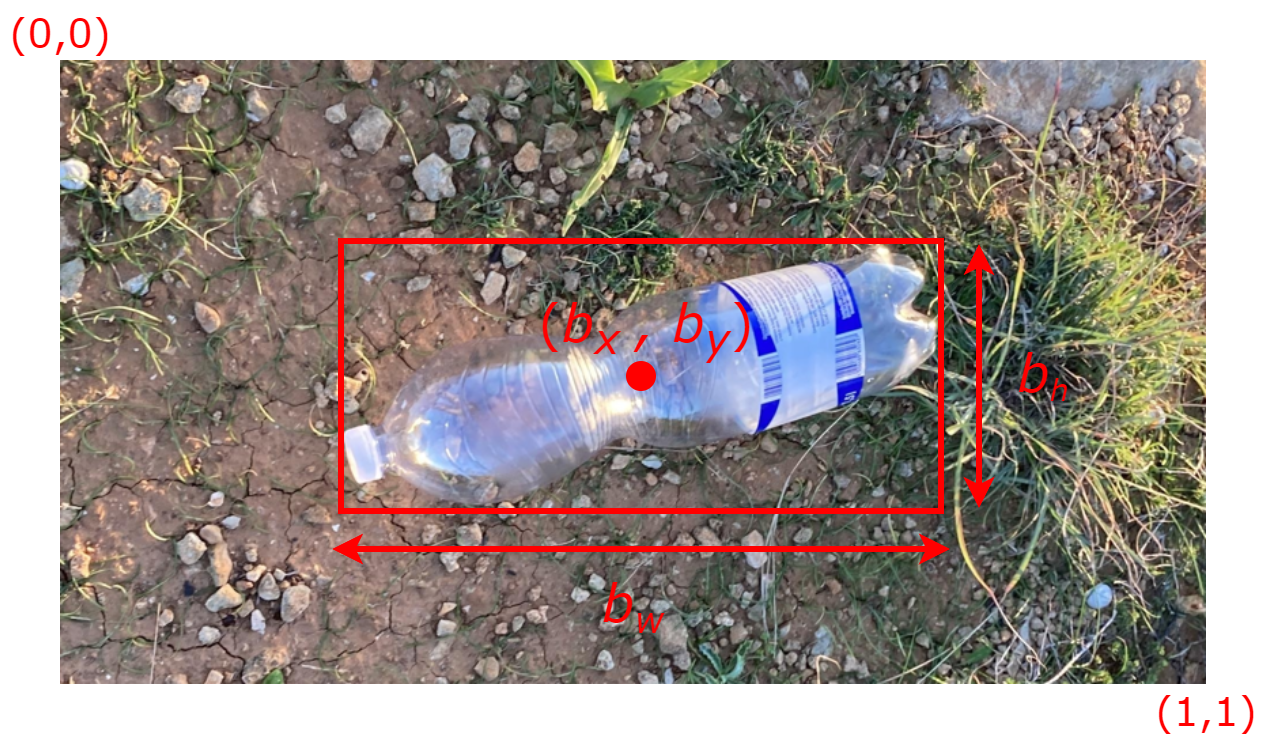
\includegraphics[width=0.7\columnwidth]{detection_explanation.png}
    \caption{Visual representation of the bounding box coordinate system on a modified image taken from the SODA dataset. (Source: \cite{soda_dataset}).}
    \label{fig:detection_explanation}
\end{figure}

\subsection{Object Classification}
\label{subsec:2_classification}

While a bounding box indicates the location of an object, identifying the type of object detected is equally important. The result of the object classification task is usually presented as a label, which denotes the class or category assigned to the detected object from a predefined set of categories. Typically, alongside the label, the outputs from detection models also include a confidence score, indicating the degree of certainty that the object belongs to the assigned category \cite{od_2}. Figure \ref{fig:classification_explanation} provides a visual example of the classification and localisation tasks, illustrating multiple detections across different categories.

\begin{figure}[!htbp]
    \centering
    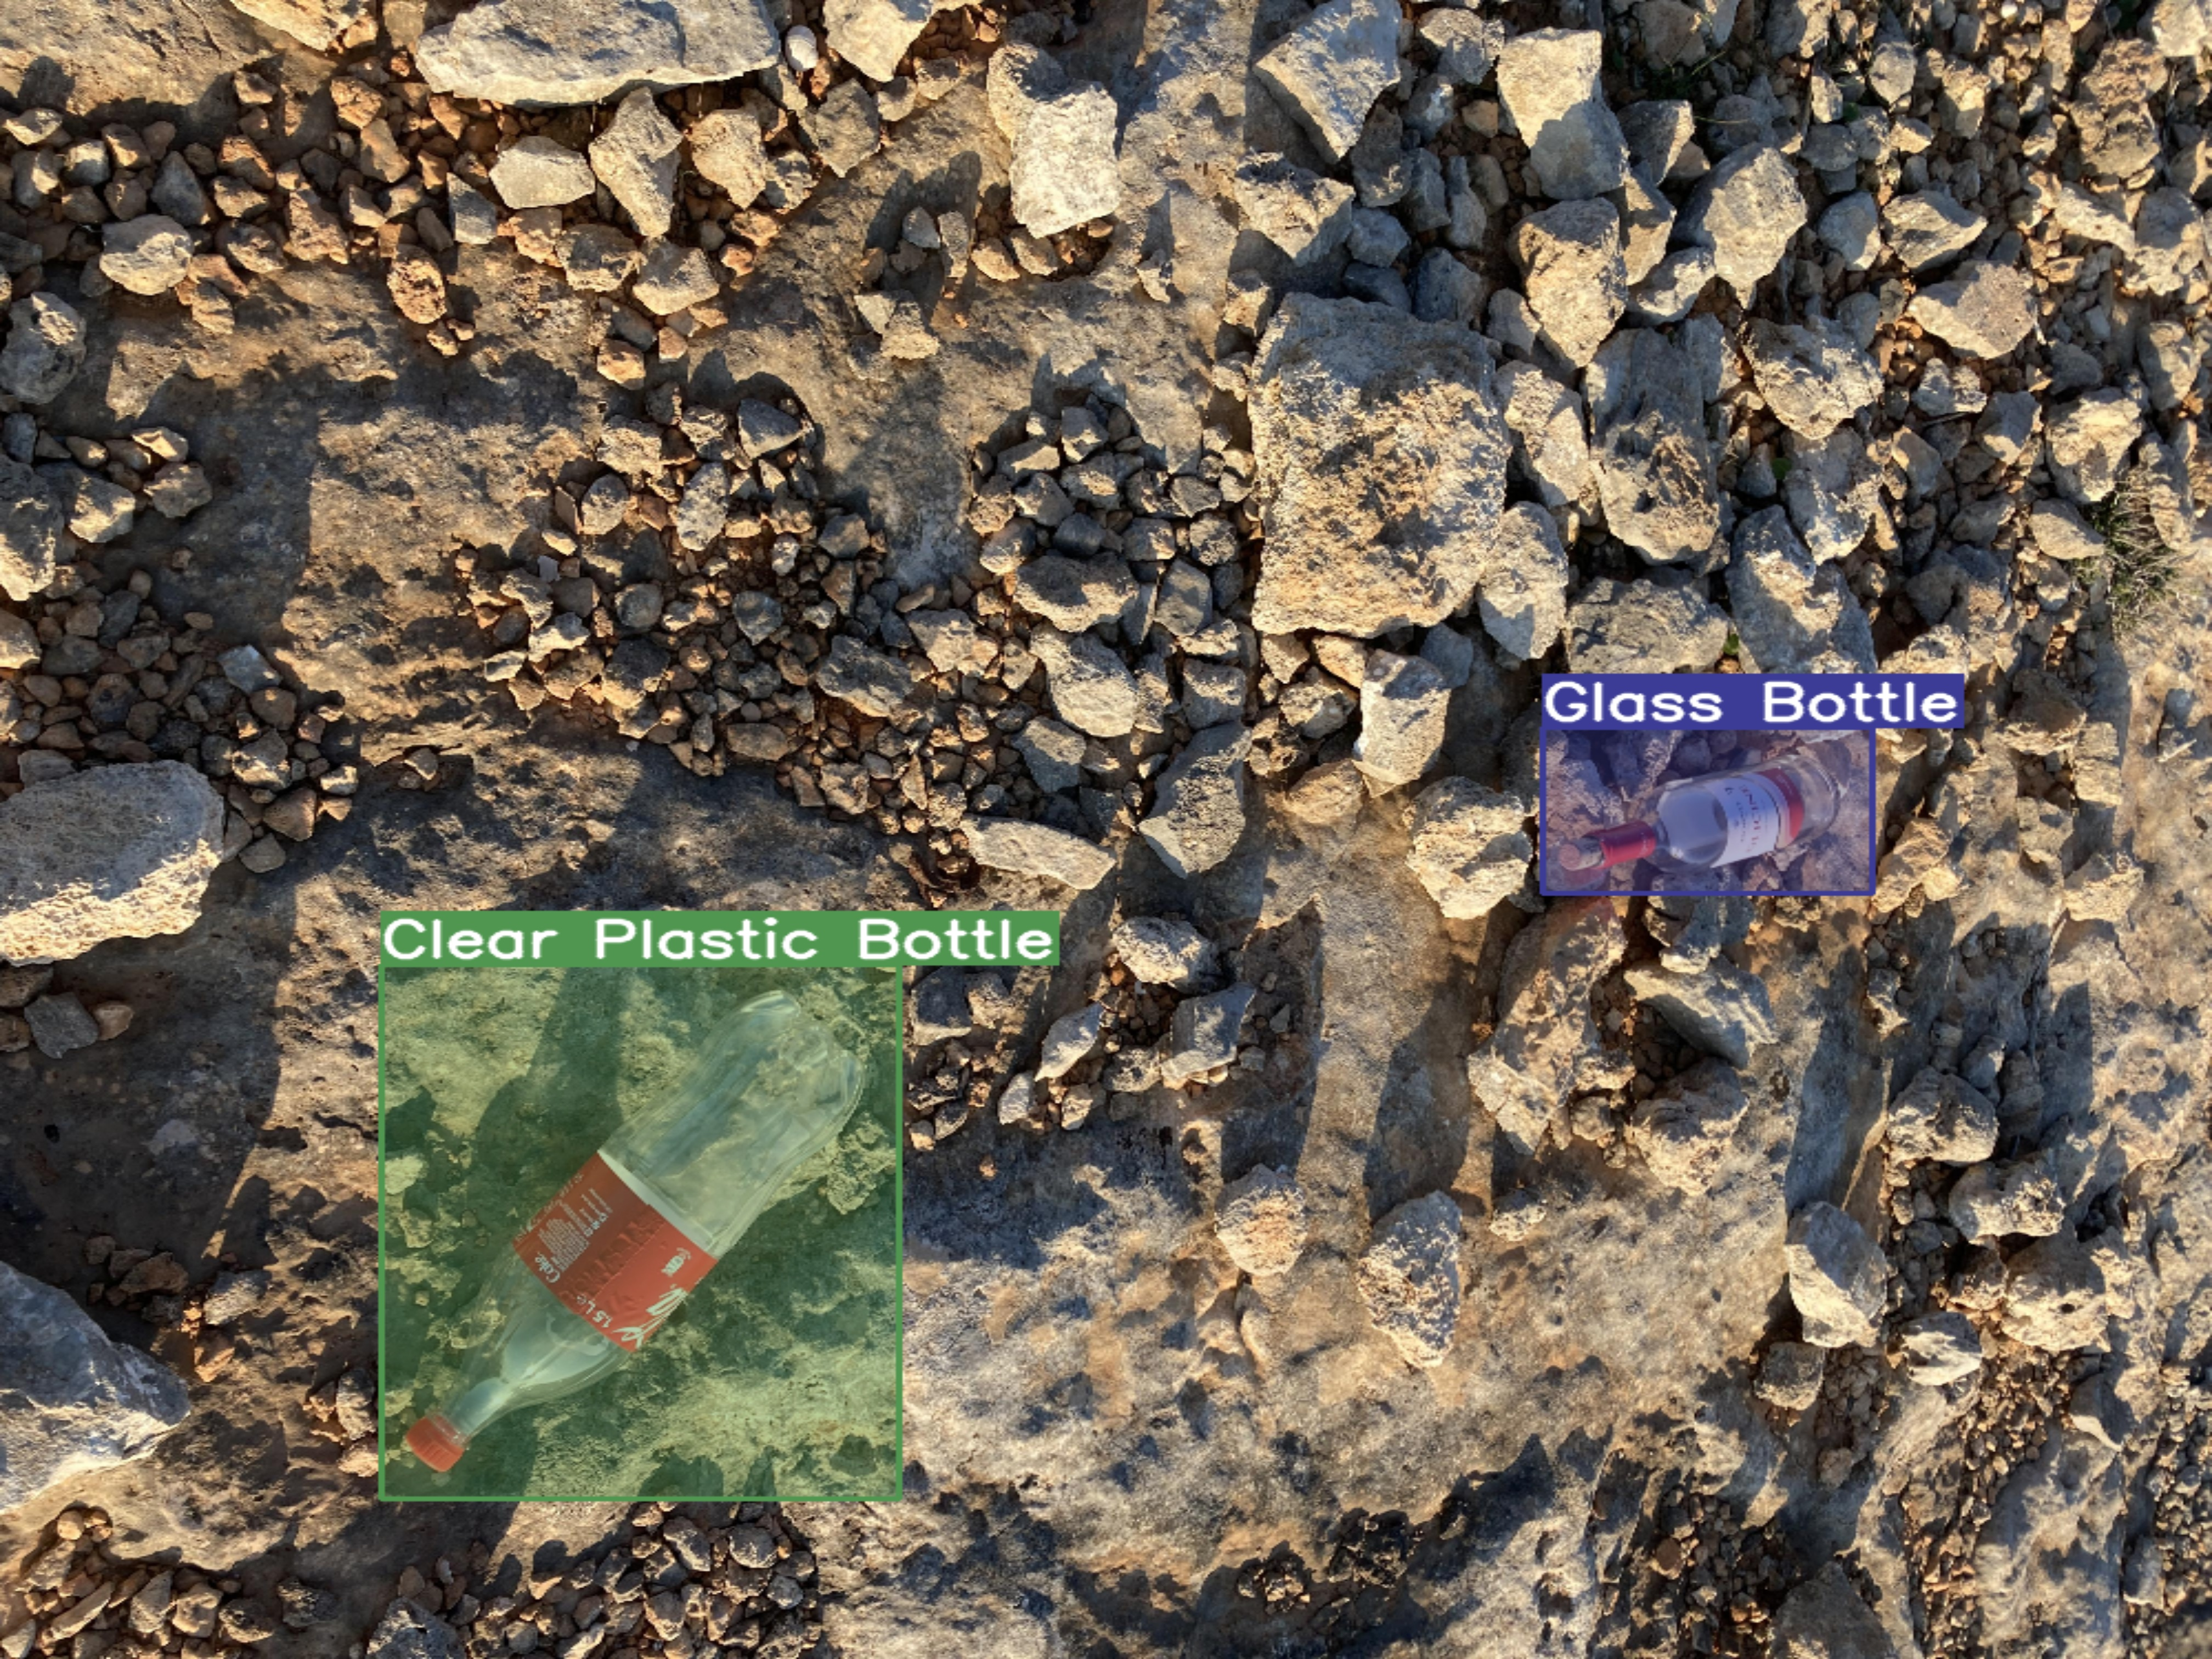
\includegraphics[width=0.7\columnwidth]{detection_soda.jpg}
    \caption{Visual representation of the classification and localisation tasks, showing multiple detections across various categories, based on an image from the SODA dataset. (Source: \cite{soda_dataset}).}
    \label{fig:classification_explanation}
\end{figure}

\subsection{Challenges in Object Detection}
\label{subsec:2_challenges}

Although the object detection problem can be divided into two subproblems and may initially seem straightforward, it is far from simple. Developing models capable of robustly detecting multiple objects across a variety of images with diverse backgrounds is a highly complex task. Furthermore, it is crucial to consider the demands of computational efficiency and real-time performance, as these factors are integral to the practical application of detection models. As highlighted by \cite{od_survey_problems}, the object detection problem encompasses several key challenges:

\begin{enumerate}[label=\textbf{\arabic*.}]
    \item \textbf{Complex Backgrounds and Interferences}: In real-world situations, especially in outdoor environments, backgrounds tend to be complex and cluttered \cite{od_survey_problems, od_2}. Natural settings introduce factors such as weather conditions, lighting changes, shadows, and occlusions, which blur the distinction between objects and their surroundings, complicating the detection process \cite{four_pillars_od}. Furthermore, the wide range of object categories and shapes adds another layer of difficulty, as different detectors may categorise the same object in varying ways. In dynamic environments, objects within the same category can appear in different poses, necessitating that object detectors generalise effectively \cite{od_survey_problems}.

    \item \textbf{Scale Variability}: Objects in real-world images often appear at varying scales. For instance, in aerial imagery, litter may appear much smaller compared to close-up photographs. Additionally, the size disparity between different types of litter, such as a glass bottle and a cotton bud, further complicates detection. Designing an algorithm that can effectively manage multi-scale variations and generate multi-scale feature representations remains a significant challenge. To this end, such tasks typically require techniques like multi-scale input processing for robust detection \cite{od_survey_problems, four_pillars_od}.

    \item \textbf{Object Occlusion}: Object occlusion presents another common challenge in detection tasks and can be classified into \textit{partial occlusion} and \textit{complete occlusion} \cite{od_survey_problems, od_problem, survey_od_2}. Complete occlusion is particularly problematic, as it prevents the detector from extracting sufficient feature information, thus diminishing detection accuracy \cite{od_survey_problems}. In contrast, partial occlusion, while less severe, still results in parts of the object being obscured by noise, which leads to a loss of important feature information and a weaker feature representation.

    % \item \textbf{Computational Efficiency and Real-Time Performance}: Object detection models are often computationally intensive due to the large number of parameters involved. Achieving high detection speed while maintaining accuracy is an ongoing challenge, especially for real-time applications.  

    \item \textbf{Class Imbalance and Dataset Bias}: In supervised learning, object detection models rely on labelled datasets, where annotators identify object locations using bounding boxes. These labelled images are then employed to train the detection algorithm. However, datasets often suffer from class imbalances, with certain object categories being over-represented while others are under-represented. This imbalance can impair model performance, particularly when detecting less frequent objects \cite{od_survey_problems}. As noted by \cite{imbalance}, class imbalance manifests in two forms: \textit{foreground-background imbalance}, where background pixels dominate over object pixels, and \textit{foreground-foreground imbalance}, where some object categories are more prevalent than others. Both types of imbalance can hinder the model’s ability to accurately detect objects, especially in complex scenes \cite{od_survey_problems, imbalance}.

    \item \textbf{Small Object Detection}: Small objects occupy only a small number of pixels within an image, which makes it difficult for models to extract meaningful features. Accurate localisation is essential, as even minor deviations in bounding box predictions can result in detection failures \cite{od_survey_problems}. Furthermore, the limited feature representation of small objects, coupled with a lack of sufficient contextual information and an inadequate number of positive examples (\textit{foreground-background imbalance}), exacerbates the challenge of detecting such objects \cite{small_detection_survey, four_pillars_od}. 
\end{enumerate}

\subsection{Object Detection Before the Rise of Deep Learning}
\label{subsec:2_detection_pre_dl}

In efforts to address the object detection problem and its associated challenges, numerous approaches were developed using traditional and machine learning methods, preceding the widespread adoption of deep learning techniques.

\subsubsection{Traditional Methods}
\label{subsubsec:2_traditional}
% \noindent \textbf{Traditional Methods:}
Early methods for object detection were heavily reliant on creative heuristics and the efficiency of basic computational techniques. Simple strategies, such as background subtraction \cite{garcia2020background}, sought to identify objects by detecting fluctuations in pixel intensity across an image. As research progressed, more sophisticated feature-driven approaches emerged. One notable example was the development of Haar cascade classifiers \cite{vinh2020real, javed2022human}, designed particularly for face detection. These classifiers exploited Haar-like features, which captured essential edge and line structures within images.
Another prominent method introduced at the time was the \gls{hog} descriptor \cite{dalal2005histograms, bhattarai2023histogram}, which was widely applied to tasks such as pedestrian detection. \gls{hog} focused on the distribution of local gradient directions, capturing the shape and appearance of objects through structured edge information.

Alongside these developments, several feature extraction techniques became foundational. The \gls{sift} \cite{lowe2004distinctive} algorithm identifies distinctive keypoints within an image by detecting local extrema in a scale-space constructed from \gls{dog}, allowing for reliable feature matching under variations in scale and rotation. The \gls{surf} algorithm \cite{bay2006surf} built upon these ideas, offering a faster alternative while maintaining reliable performance under transformations such as viewpoint and illumination changes.
Later, the \gls{orb} algorithm \cite{rublee2011orb} emerged, combining the efficiency of the \gls{fast} keypoint detector with the compactness of the \gls{brief} descriptor. \gls{orb} provided a computationally inexpensive, rotation-invariant solution, serving as a competitive alternative to \gls{sift} and \gls{surf} in environments requiring faster performance.

\subsubsection{Machine Learning Approaches}
\label{subsubsec:2_machine_learning}

In tandem with traditional methods, notable advances in object detection were made through the adoption of \gls{ml}, a branch of \gls{ai} focused on enabling systems to learn patterns from data \cite{machine_learning}. During this period, \gls{svms} \cite{hearst1998support} emerged as a pivotal tool, providing a strong classification framework, specifically when combined with feature descriptors such as \gls{hog} \cite{bhatt2023state}. Other machine learning strategies also contributed meaningfully to the field's development. Boosting algorithms, such as \gls{adaboost}, proved instrumental in the Viola-Jones face detection framework \cite{viola2001rapid}, while ensemble methods, including \gls{rf} \cite{saffari2009line} and techniques utilising \gls{rgbd} information \cite{seychell16}, further expanded detection capabilities. Although these approaches improved performance by allowing models to learn directly from data, they continued to rely heavily on manually engineered features. Additional progress was marked by the introduction of \gls{dpm} \cite{felzenszwalb2009object}, which conceptualised objects as collections of interconnected parts, thus enabling more effective modelling of variations in object appearance. Collectively, these machine learning-based methods significantly advanced object detection, laying the essential foundations for the subsequent development of deep learning approaches.

\subsection{Object Detection in the Era of Deep Learning}
\label{subsec:2_detection_in_dl}

The introduction of \gls{dl}, most notably \gls{cnn}, brought about a fundamental shift in the field of object detection \cite{cnn_survey}. In contrast to earlier methods that depended heavily on labour-intensive, hand-crafted feature engineering, \gls{cnn} are capable of automatically extracting features from large datasets, thereby streamlining the detection process and improving overall efficiency \cite{feature_learning, deep_learning_review, cnns}. This progression led to the development of a new generation of object detectors that demonstrated greater accuracy and reliability than their traditional counterparts. Consequently, numerous object detection architectures have been introduced, each offering distinct advantages and facing particular limitations.

CNN-based object detectors are generally categorised into two principal types: one-stage detectors and two-stage detectors \cite{one_two_stage_detection}. More recently, transformer-based models, originally proposed for natural language processing tasks \cite{transformers}, have been successfully adapted for computer vision applications, including object detection \cite{detr, rt-detr}, pushing performance boundaries even further. Beyond these mainstream approaches, emerging deep learning models increasingly incorporate visual attention mechanisms to strengthen feature representation and contextual reasoning within images \cite{bartolo2024correlationobjectdetectionperformance, va_detection}. Moreover, alternative paradigms, such as \gls{rl}, have also been explored to dynamically optimise object detection strategies \cite{bartolo2024integratingsaliencyrankingreinforcement, Caicedo_2015_ICCV}.

% In the sections that follow, we review one-stage detectors, two-stage detectors, transformer-based detectors, as well as approaches that do not fit neatly within these established categories.

\subsubsection{One Stage Detectors}
\label{subsubsec:2_onestage}

One-stage detectors address the problem of object detection by concurrently performing localisation and classification within a single network, predicting bounding boxes and corresponding labels in a single forward pass.
OverFeat \cite{overfeat}, introduced in 2013, marked an early application of deep learning to object detection. It employed a multi-scale sliding window method wherein a classifier generated class labels and confidence scores at each spatial location. Prediction quality was subsequently improved through adjustments in resolution and the merging of bounding boxes.

The You Only Look Once (YOLO) series significantly reshaped one-stage detection by reframing object detection as a regression problem. The original \gls{yolo} model \cite{yolo}, released in 2016, partitioned images into an $S \times S$ grid, with each cell responsible for predicting bounding boxes, confidence scores, and class probabilities (refer to Figure \ref{fig:yolov1}). Later versions introduced several refinements: \gls{yolo}v2 \cite{yolov2} integrated batch normalisation and optimised anchor boxes; \gls{yolo}v4 \cite{yolov4} adopted a suite of training techniques commonly referred to as bag-of-freebies \cite{bagoffreebies}; \gls{yolo}v5 \cite{yolov5} incorporated automatic anchor learning; and \gls{yolo}X \cite{yolox} shifted towards anchor-free methodologies. More recently, \gls{yolo}v12 \cite{yolov12} introduced attention-driven designs, leveraging linear attention mechanisms and residual-efficient layer aggregation networks.

Further adaptations have continued to emerge. For example, \gls{yolo}-NAS \cite{yolonas} improved detection efficiency by employing \gls{nas} within a quantisation-friendly framework. Meanwhile, \gls{yolo}-World \cite{yoloworld} extended the model’s capabilities to open-vocabulary detection, integrating vision-language path aggregation and region-text contrastive loss, achieving notable performance boosts in both speed and accuracy over contemporary models.

\begin{figure}[ht]
    \centering
    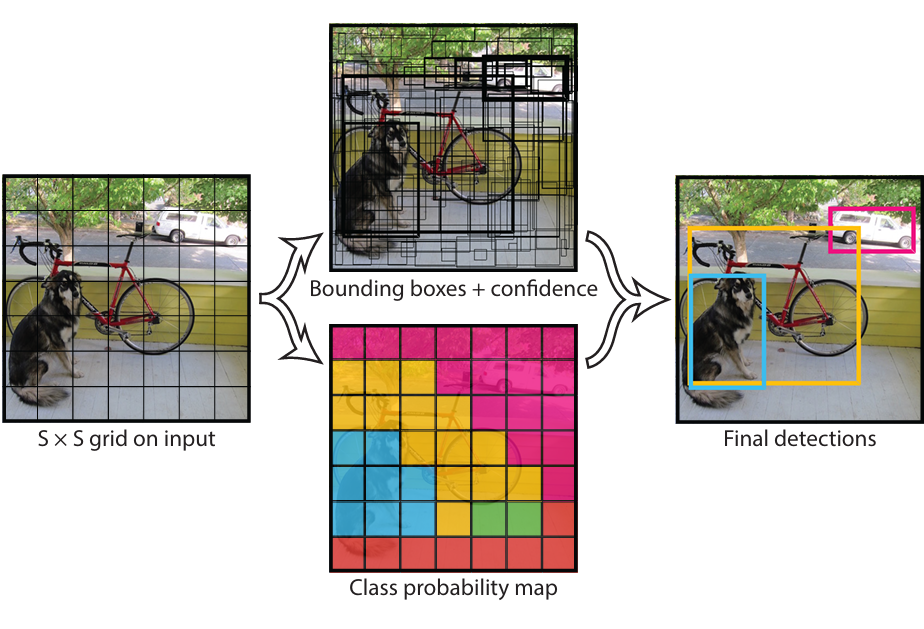
\includegraphics[width=0.7\linewidth]{yolov1.png}
    \caption{YOLOv1 pipeline. (Source: \cite{yolo})}
    \label{fig:yolov1}
\end{figure}

In parallel with developments in \gls{yolo}, other notable one-stage detectors have emerged. Among them, the \gls{ssd} \cite{ssd}, released in 2016, introduced an architecture that bypasses region proposal networks. Instead, it predicts object categories and bounding box refinements directly over a fixed set of predefined anchor boxes, known as default boxes.
\gls{ssd} builds on a modified VGG-16 backbone, where the fully connected layers are removed and replaced with additional convolutional layers. These progressively reduce spatial resolution, resulting in multiple feature maps of decreasing size. Each feature map is responsible for detecting objects at a specific scale, supporting effective multi-scale detection.

To accommodate objects of varying sizes, \gls{ssd} deploys default boxes with multiple aspect ratios and scales across each feature map. At every level, lightweight convolutional heads independently predict class labels and refine bounding box coordinates. These operations are performed in parallel across all scales, enabling the model to classify and localise objects within a single forward pass simultaneously. This design achieves an effective compromise between computational efficiency and detection accuracy. The complete architecture is illustrated in Figure~\ref{fig:ssd}.

\begin{figure}[!htbp]
\centering
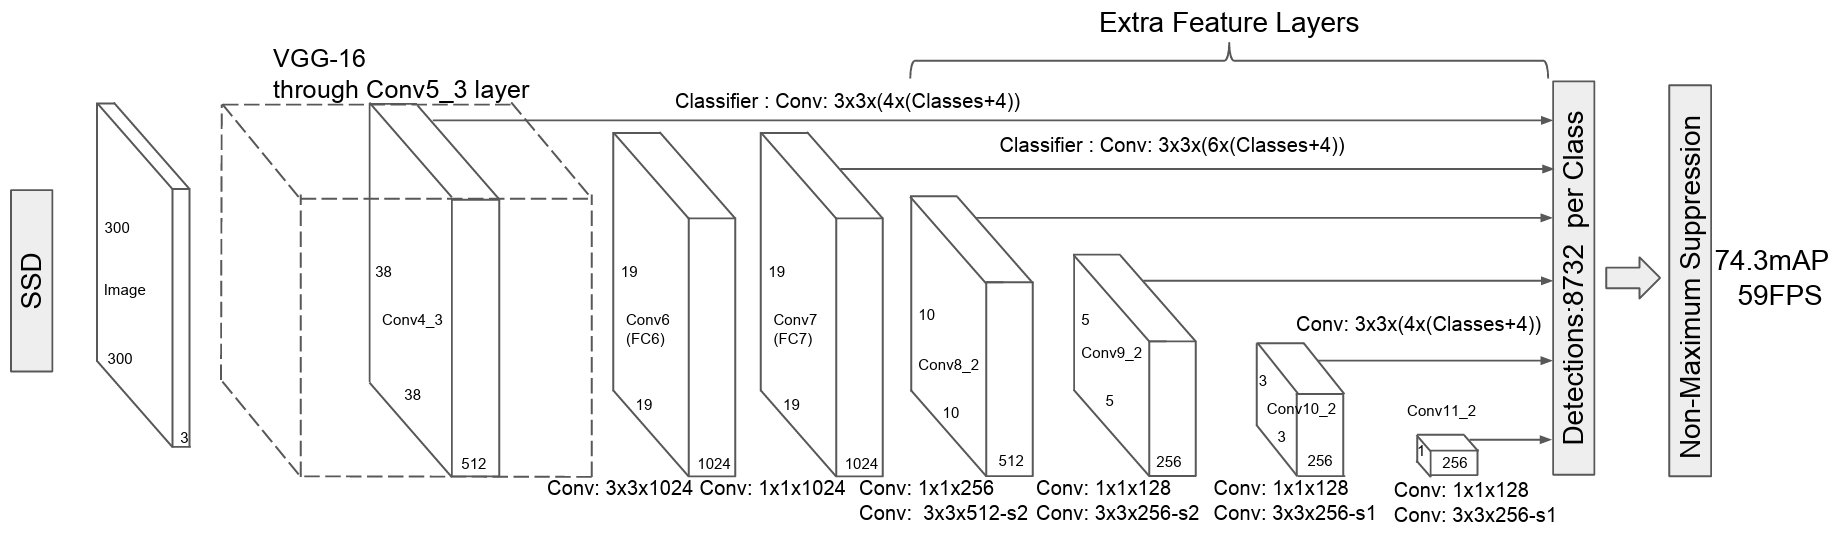
\includegraphics[width=1\columnwidth]{ssd1.png}
\caption{SSD architecture. (Source: \cite{ssd})}
\label{fig:ssd}
\end{figure}

Other prominent one-stage detectors include RetinaNet \cite{retinanet}, introduced in 2017 to mitigate the foreground–background class imbalance that commonly undermines the performance of dense object detectors. Unlike two-stage methods such as Faster \gls{rcnn}, RetinaNet performs classification and localisation in a single forward pass (see Figure~\ref{fig:retinanet}). It employs a ResNet backbone combined with a \gls{fpn} to extract multi-scale features, followed by two parallel subnetworks: one for predicting object classes and another for refining bounding box coordinates. A key innovation is the use of focal loss, which shifts training focus toward difficult, misclassified examples by down-weighting easy negatives. To detect objects of different shapes and sizes, RetinaNet utilises anchor boxes with varying scales and aspect ratios across feature levels. This design allows the model to achieve accuracy comparable to that of many two-stage detectors, while maintaining the efficiency advantages of a single-stage framework.

\begin{figure}[!htbp]
\centering
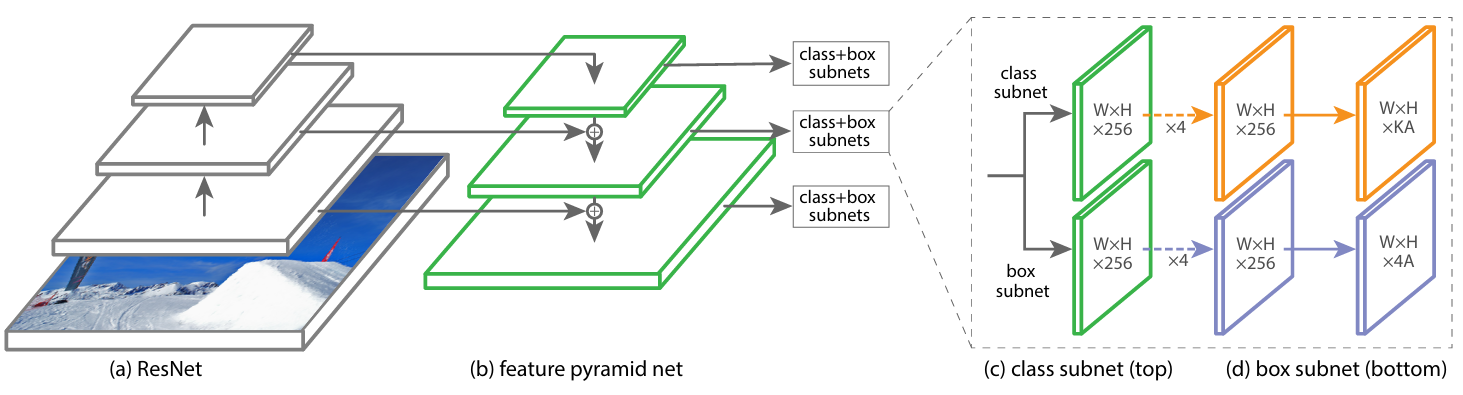
\includegraphics[width=1\columnwidth]{retinanet.png}
\caption{RetinaNet architecture. (Source: \cite{retinanet})}
\label{fig:retinanet}
\end{figure}


Building on the foundation of \gls{ssd}, SSDLite was introduced in 2018 as a lighter variant designed for mobile and resource-constrained devices \cite{ssdlite}. It replaces the original \gls{ssd}'s VGG-16 backbone with MobileNetv2, which employs inverted residual layers and linear bottlenecks to balance efficient feature extraction with model capacity. This change significantly reduces computational demand. Furthermore, standard convolutional layers in the detection heads are substituted with depthwise separable convolutions (see Figure~\ref{fig:ssdlite}), which decrease parameter count and speed up inference. Later iterations incorporated MobileNetv3 as the backbone, adding squeeze-and-excitation modules and the h-swish activation function for improved efficiency and accuracy (see Figure~\ref{fig:ssdlite2}). These adaptations make SSDLite highly suitable for deployment in environments with limited computational resources.

\begin{figure}[!htbp]
\centering
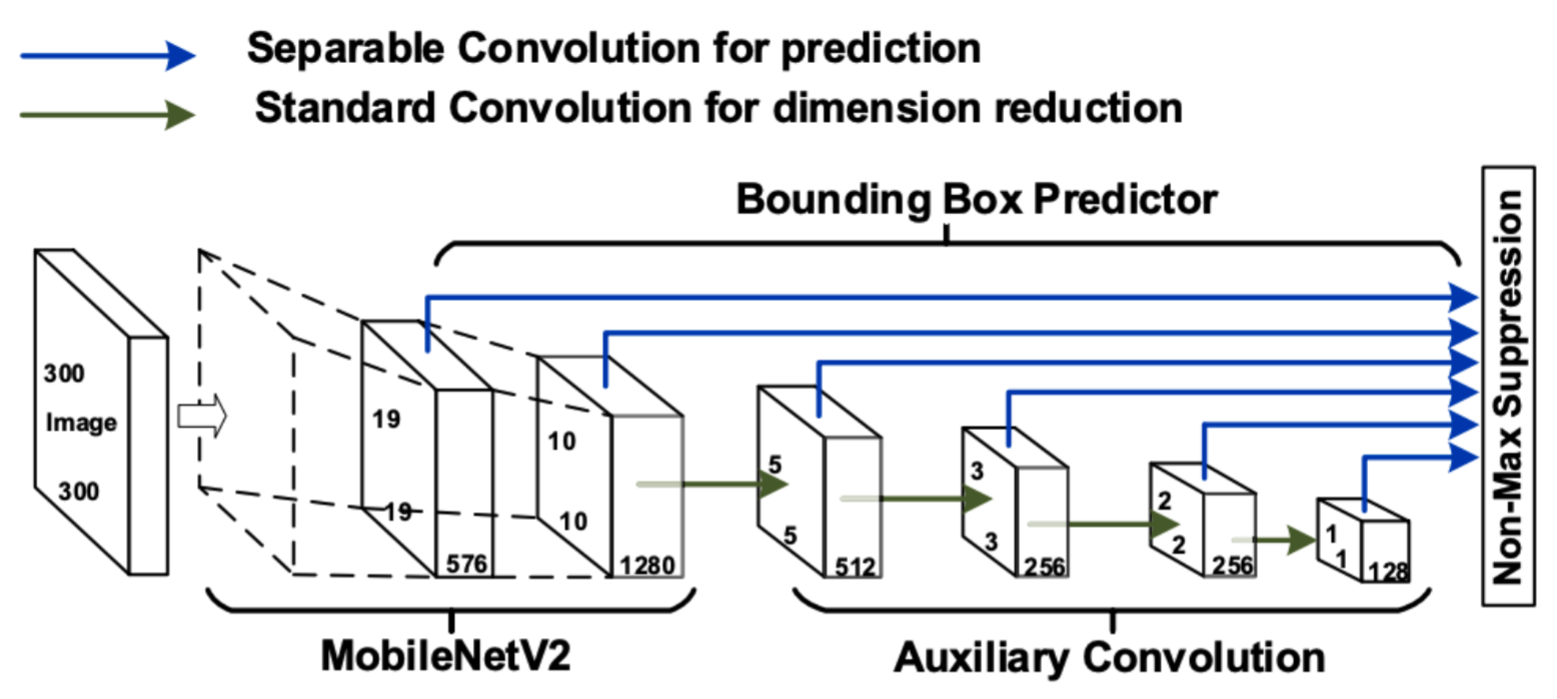
\includegraphics[width=0.8\columnwidth]{ssdlite.png}
\caption{MobileNetV2-SSDLite architecture. (Source: \cite{ssdlite_diagram})}
\label{fig:ssdlite}
\end{figure}

\begin{figure}[!htbp]
\centering
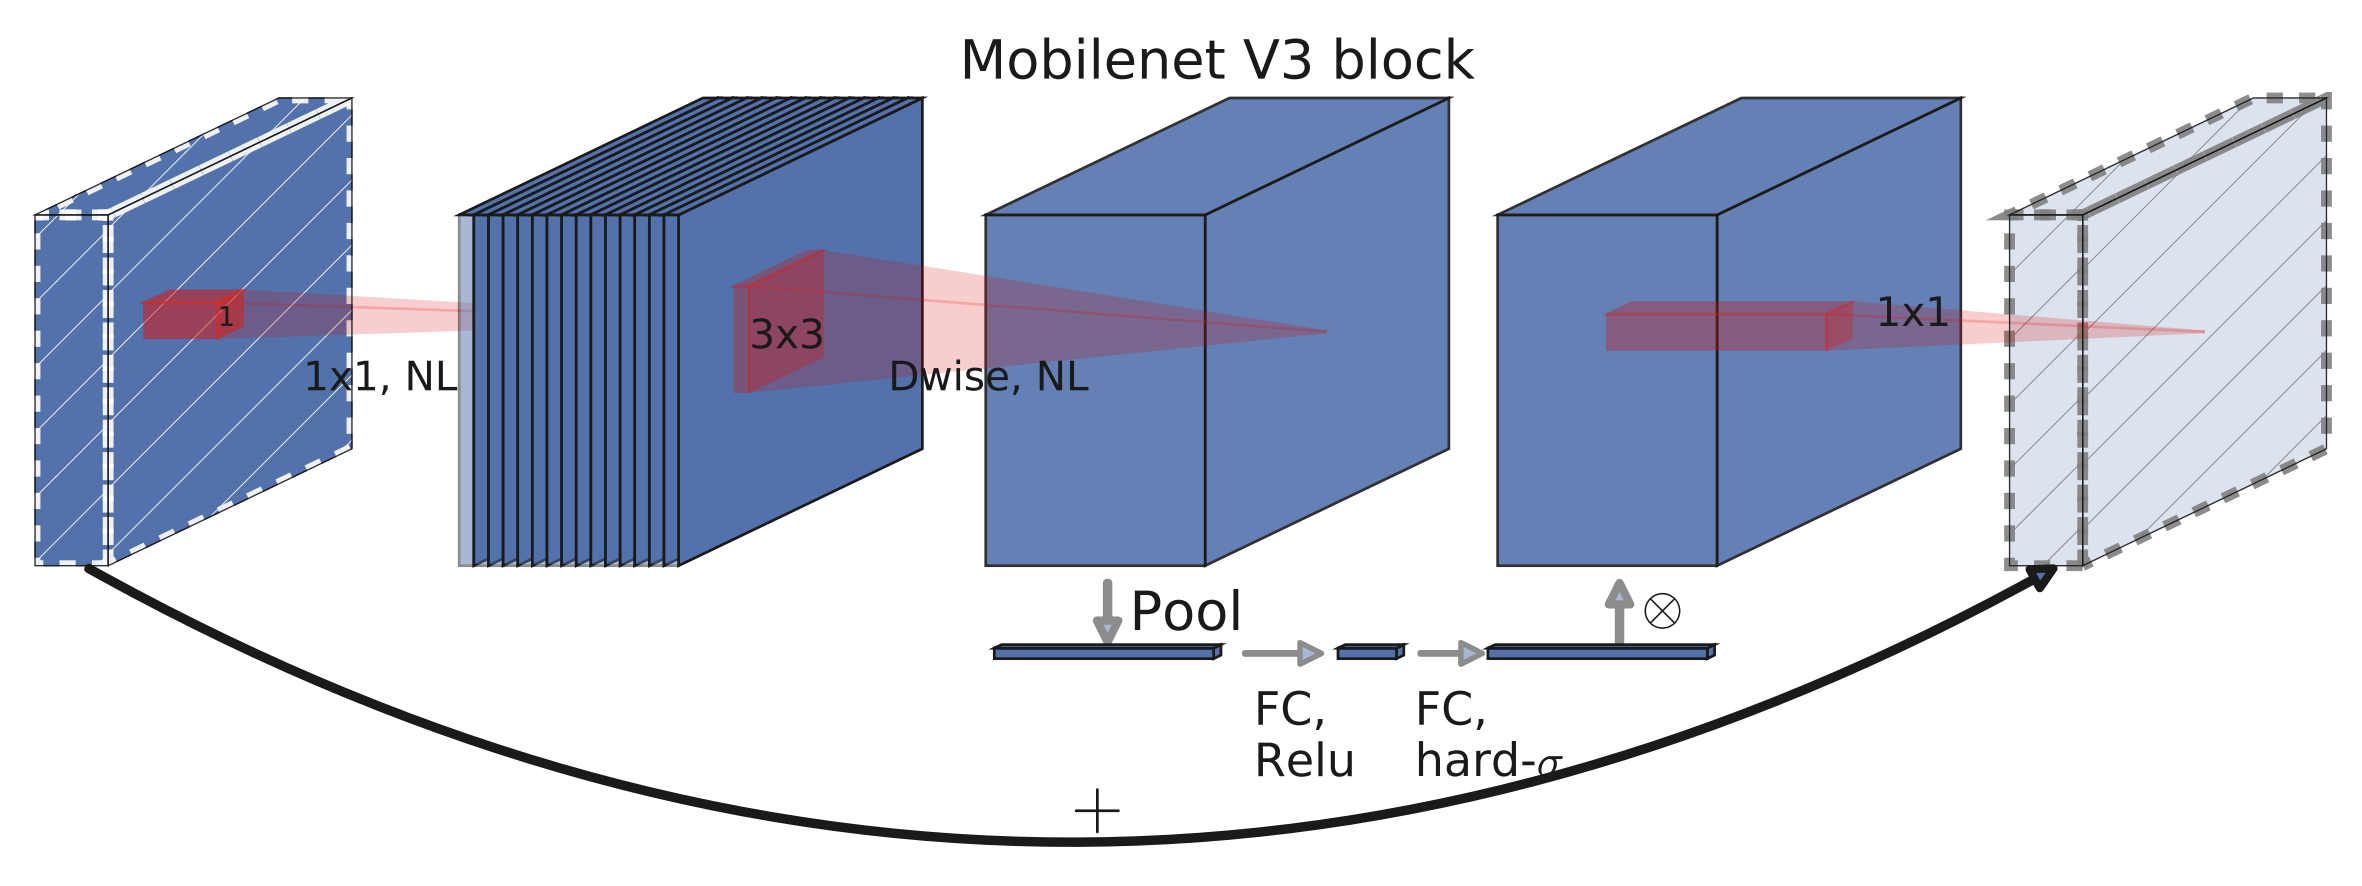
\includegraphics[width=0.9\columnwidth]{mobilenet-v3-block.png}
\caption{MobileNetv3 architecture. (Source: \cite{mobilenetv3})}
\label{fig:ssdlite2}
\end{figure}

In contrast, \gls{fcos} \cite{fcos}, released in 2019, departs from traditional anchor box approaches entirely. It adopts a fully convolutional architecture that directly predicts object centre points and bounding box coordinates, simplifying the detection pipeline. One distinctive feature is the addition of a centre-ness branch, which estimates how close a predicted box is to the actual object centre, helping suppress low-quality detections and reducing false positives (see Figure~\ref{fig:fcos}). Built on a ResNet-\gls{fpn} backbone, \gls{fcos} leverages multi-scale feature extraction to improve detection across object sizes. Its output head consists of three branches: regression for bounding boxes, classification for object categories, and centre-ness for quality estimation, enabling competitive performance without complex anchor matching.

\begin{figure}[!htbp]
\centering
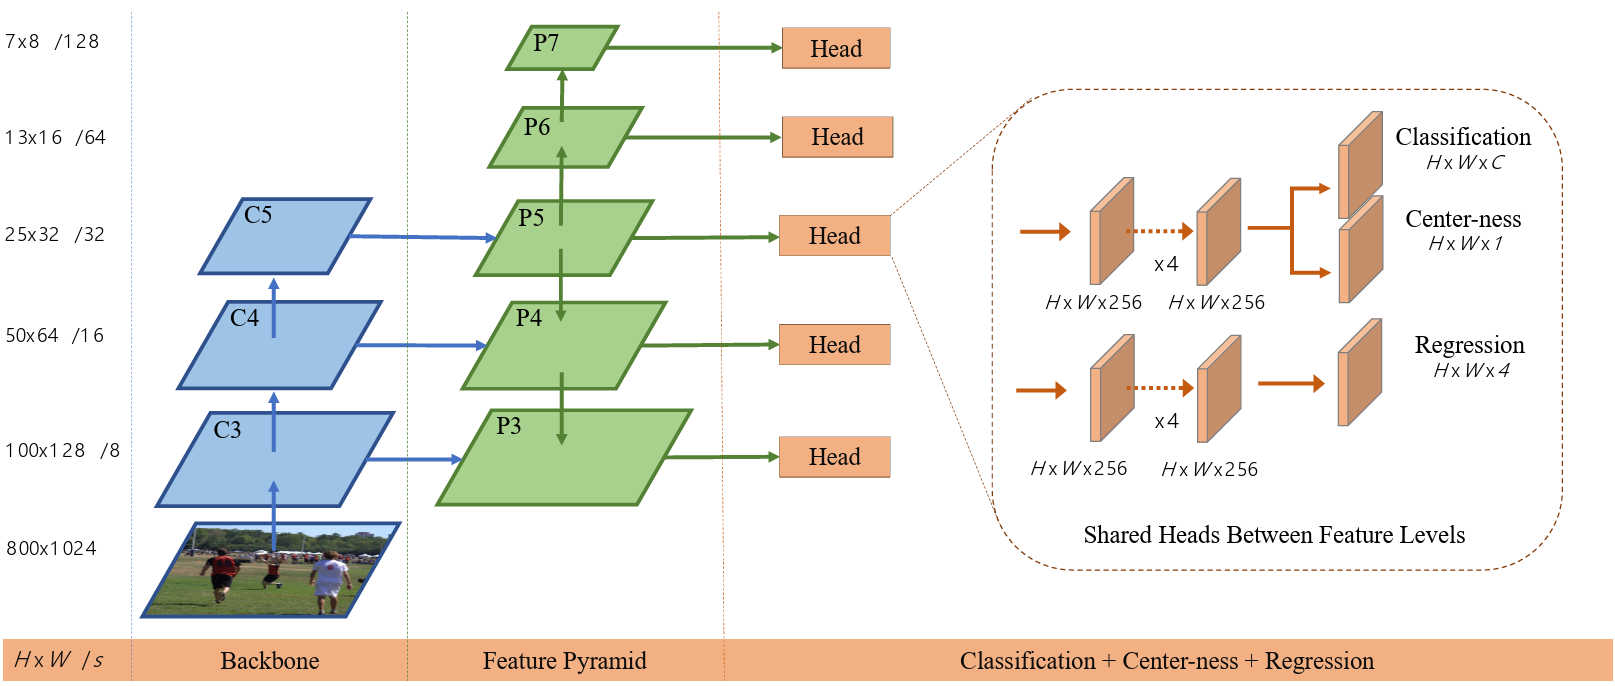
\includegraphics[width=1\columnwidth]{fcos.png}
\caption{FCOS architecture. (Source: \cite{fcos})}
\label{fig:fcos}
\end{figure}

\subsubsection{Two Stage Detectors}
\label{subsubsec:2_twostage}

In contrast to one-stage detectors, two-stage detectors separate region proposal from classification and localisation. The \gls{rcnn} family was instrumental in this approach, beginning with the original \gls{rcnn} model \cite{rcnn}. This model used a selective search to generate candidate regions, which were then passed individually through AlexNet \cite{alexnet} to extract features. Each region was classified and refined through fully connected layers. Although effective, this process was slow due to repeated feature extraction for each region (see Figure \ref{fig:rcnn}). Fast \gls{rcnn} \cite{fastrcnn} improved efficiency by computing a convolutional feature map over the entire image once, and then applying region proposals on this shared feature map. This reduced redundant computations while maintaining detection accuracy.

\begin{figure}[ht]
\centering
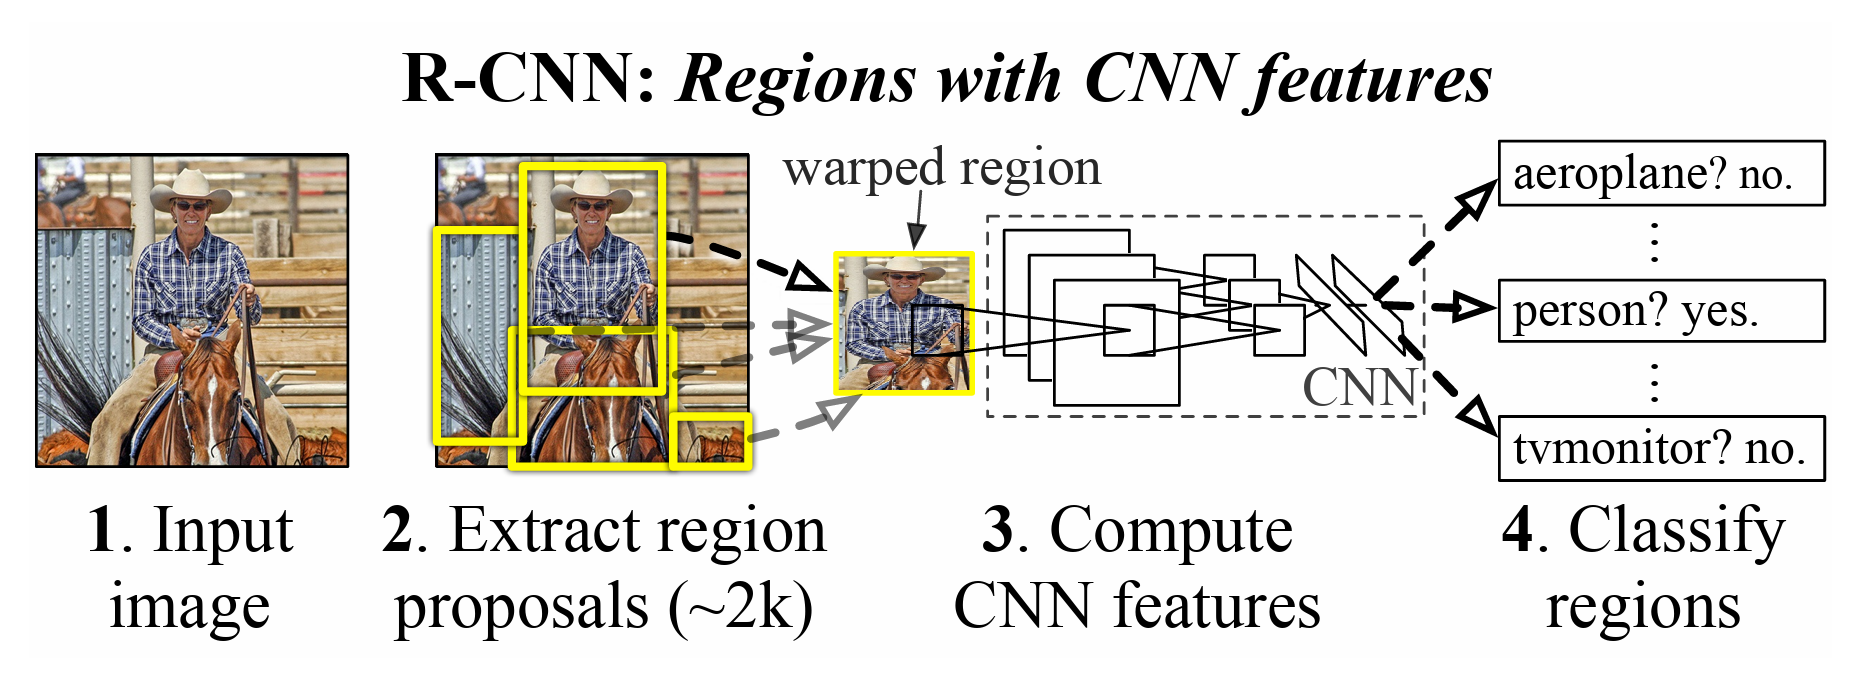
\includegraphics[width=0.9\linewidth]{content/chapters/2_background/figures/RCNN.png}
\caption{R-CNN architecture. (Source: \cite{rcnn})}
\label{fig:rcnn}
\end{figure}

A more pivotal advancement came with Faster \gls{rcnn} \cite{fasterrcnn}, which introduced the \gls{rpn}. This component removed the dependency on external region proposal algorithms by allowing the network to learn object proposals directly from feature maps using anchor boxes of varying scales and aspect ratios. The \gls{rpn} shares convolutional features with the detection network, enabling efficient and integrated region proposal generation. After region proposals are obtained, a shared head performs both classification and bounding box regression, streamlining the process within a unified framework.

% \begin{figure}[ht]
% \centering
% 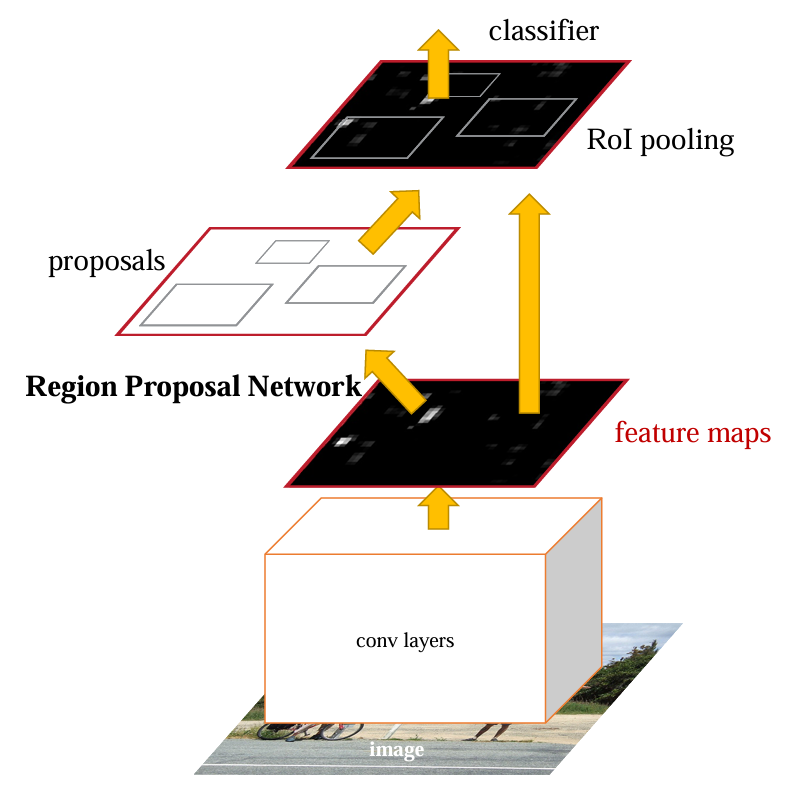
\includegraphics[width=0.5\linewidth]{fasterrcnn.png}
% \caption{Faster \gls{rcnn} pipeline. (Source: \cite{fasterrcnn})}
% \label{fig:fasterrcnn}
% \end{figure}

Subsequent improvements to Faster \gls{rcnn} incorporated an \gls{fpn}, significantly enhancing the model’s ability to detect objects at multiple scales by enriching feature representations across layers. This advancement became standard in later implementations, exemplified by the ResNet-\gls{fpn} backbone architecture. Here, a shared network efficiently performs both region proposal and detection tasks. After extracting region proposals, a unified head simultaneously executes classification and bounding box regression, preserving architectural simplicity while boosting efficiency. Building upon this foundation, Mask \gls{rcnn} \cite{maskrcnn} added a parallel branch to predict segmentation masks for each \gls{roi}, enabling instance segmentation alongside detection.

\begin{figure}[!htbp]
\centering
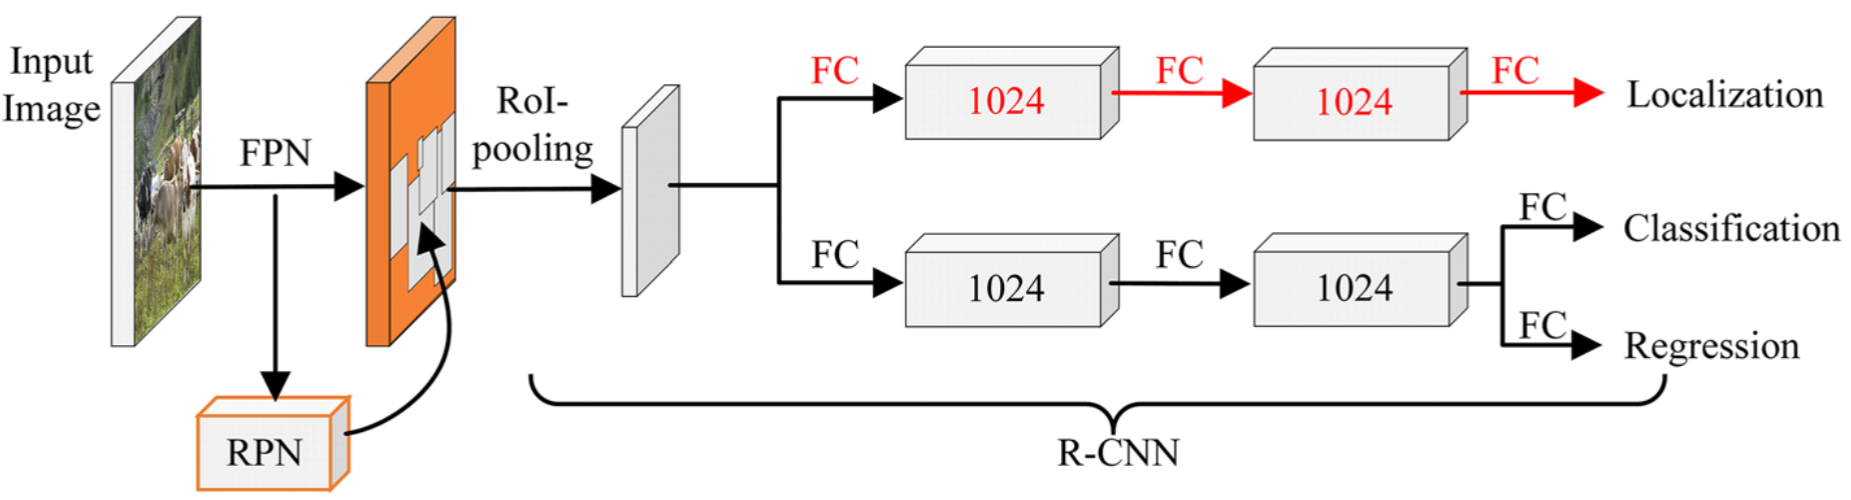
\includegraphics[width=1\columnwidth]{fasterrcnn2.png}
\caption{Faster \gls{rcnn} architecture with ResNet-50 backbone and integrated \gls{fpn}, demonstrating a unified two-stage detection pipeline for proposal generation, classification, and bounding box regression. (Source: \cite{fasterrcnn_diagram})}
\label{fig:fasterrcnn2}
\end{figure}

Complementing these technological advancements, \gls{fpn} \cite{fpn} improved detection across all network layers by constructing a feature pyramid for improved multi-scale detection. This pyramid included bottom-up pathways that captured semantic information and top-down pathways that refined these maps by merging high-level features with spatially rich information. The \gls{rfcn} \cite{rfcn} integrated both classification and localisation tasks, utilising position-sensitive score maps to classify and refine bounding box coordinates. This approach struck a balance between speed and accuracy by enabling shared computation across regions.
Building on these two-stage frameworks, EfficientDet \cite{efficientdet} incorporated an EfficientNet \cite{efficientnet} backbone and employed a weighted bi-directional \gls{fpn} for efficient multi-scale feature fusion (see Figure \ref{fig:efficientdet}). Furthermore, it introduced a compound scaling method that uniformly scaled resolution, depth, and width across the backbone, feature network, and prediction networks.

\begin{figure}[!htbp]
\centering
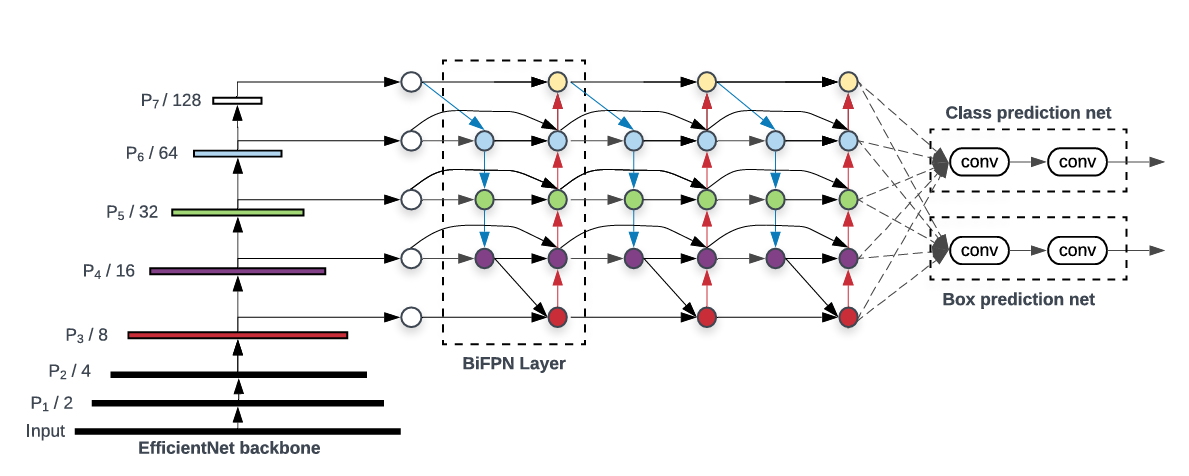
\includegraphics[width=1\columnwidth]{efficientdet.png}
\caption{EfficientDet architecture. (Source: \cite{efficientdet})}
\label{fig:efficientdet}
\end{figure}

\subsubsection{Transformer-Based Detectors}
\label{subsubsec:2_transformers}

Transformers, originally developed for natural language processing \cite{transformers}, have garnered significant attention in computer vision \cite{visiontransformer}, especially for object detection tasks. The \gls{detr} \cite{detr}, introduced in 2020, marked a pioneering shift in transformer-based object detection by framing the task as a set prediction problem. \gls{detr} removed the need for region proposals, employing a bipartite matching loss that aligns predicted boxes with ground-truth boxes. Its encoder-decoder architecture processes input data through self-attention mechanisms, enabling it to distinguish between individual instances successfully. This architecture supports both object detection and panoptic segmentation tasks, and the architecture for \gls{detr} is illustrated in Figure \ref{fig:detr}.

\begin{figure}[ht]
    \centering
    \includegraphics[width=0.9\linewidth]{detr.png}
    \caption{DETR architecture. (Source: \cite{detr})}
    \label{fig:detr}
\end{figure}

Several models have built upon the foundation laid by \gls{detr}. The \gls{dino} framework \cite{zhang2022dino, li2022dn, liu2022dabdetr} improved both training efficiency and overall performance. Grounding \gls{dino} \cite{groundingdino} advanced zero-shot object detection by enabling the identification of objects without prior training on specific categories. This was achieved through the use of natural language queries and the multimodal fusion of textual and visual information.
Real-time transformer-based detection has also emerged as a significant advancement. The \gls{rtdetr} \cite{rt-detr} addressed the limitations of non-maximum suppression by incorporating a hybrid encoder and high-quality initial queries. This made the model more efficient and adaptable, eliminating the need for retraining. \gls{rtdetr}v2 \cite{rt-detrv2} further optimised training strategies and integrated bag-of-freebies techniques, enhancing real-time performance.

Vision-language models have also adopted transformer architectures for object detection. PaliGemma \cite{paligemma} combined a vision transformer for image encoding with a transformer decoder to merge textual and visual data, framing object detection as a set prediction task. Its successor, PaliGemma 2 \cite{paligemma2}, improved efficiency by incorporating Gemma 2 language models with the SigLIP vision encoder, enabling it to handle multiple input resolutions more effectively. Similarly, Florence-2 \cite{florence2} utilised a unified, prompt-based architecture with an image encoder and a multi-modality encoder-decoder to address a range of vision-language tasks, including object detection, captioning, and segmentation (refer to Figure \ref{fig:florence2}).
These transformer-based approaches collectively represent a paradigm shift in object detection, offering end-to-end solutions that eliminate traditional components, such as non-maximum suppression, while enabling more flexible, multimodal, and zero-shot capabilities.

\begin{figure}[!htbp]
\centering
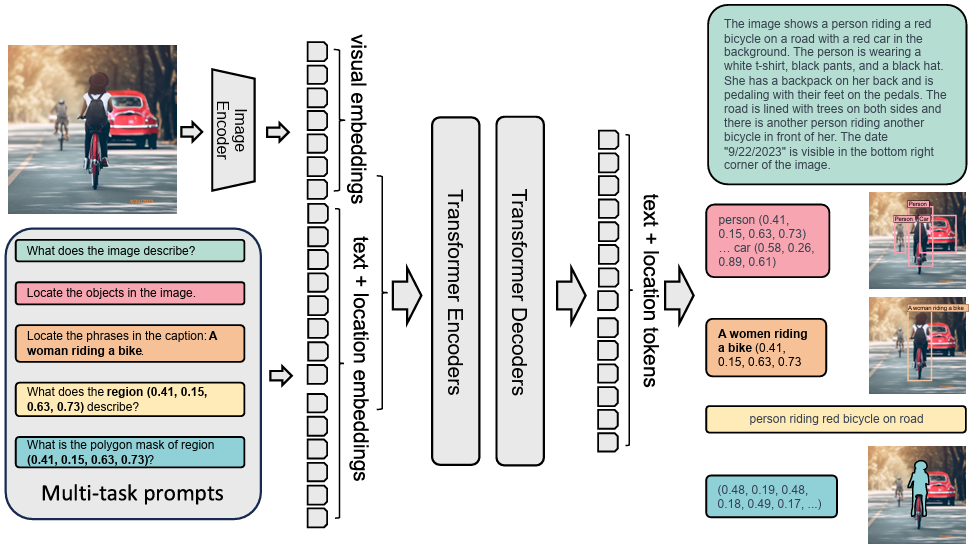
\includegraphics[width=1\columnwidth]{florence2.png}
\caption{Florence-2 architecture. (Source: \cite{florence2})}
\label{fig:florence2}
\end{figure}

\subsubsection{Other Deep Learning Approaches}
\label{subsubsec:2_other_approaches}

Deep learning methodologies that go beyond traditional one-stage, two-stage, and transformer detectors have emerged to tackle specific challenges in object detection. These approaches can be categorised based on their underlying principles and technical innovations.
One prominent paradigm is reinforcement learning-based detection frameworks, starting with the approach by Caicedo et al. \cite{Caicedo_2015_ICCV}, which used class-specific Deep Q-Network agents to iteratively refine object localisation by framing detection as a \gls{sdmp}. Subsequent studies have expanded on this foundation by incorporating multitask learning \cite{multitask_learning}, integrating saliency ranking \cite{bartolo2024integratingsaliencyrankingreinforcement}, and developing other complementary strategies \cite{reinforcenet, bar_rl} to enhance the reinforcement learning paradigm for object detection. An example architecture of such a reinforcement learning-based framework for iterative object localisation is depicted in Figure~\ref{fig:sarlvision}.

\begin{figure}[!htbp]
\centering
\includegraphics[width=1\columnwidth]{architecture.png}
\caption{Architecture of a reinforcement learning-based object detection framework for iterative object localisation. (Source: \cite{bartolo2024integratingsaliencyrankingreinforcement})}
\label{fig:sarlvision}
\end{figure}

Feature enhancement techniques represent another significant area, exemplified by \gls{dcn} introduced in 2017 \cite{dcn}. \gls{dcn} improves feature extraction across various detector architectures by incorporating deformable convolutional layers and \gls{roi} pooling, enabling adaptive sampling of input features with learnt offsets. This approach better models spatial transformations and bolsters the detection of objects with varying shapes and sizes.
Point-based and slicing-based approaches offer alternative detection paradigms. CenterNet \cite{centernet}, models objects as single points (the centres of their bounding boxes) and uses keypoint estimation to identify these centres while regressing to other properties such as size and orientation. This results in an end-to-end differentiable system that is simpler, faster, and often more accurate than traditional bounding box-based detectors. The architecture of CenterNet is illustrated in Figure~\ref{fig:centernet}. Furthermore, the \gls{sahi} framework \cite{sahi_detection} improves small object detection by dividing input images into overlapping patches during both fine-tuning and inference. This increases pixel coverage for small objects, which are then reassembled through non-maximum suppression.
These diverse approaches complement mainstream detection architectures by addressing specific limitations and introducing novel perspectives on the object detection problem.

\begin{figure}[!htbp]
\centering
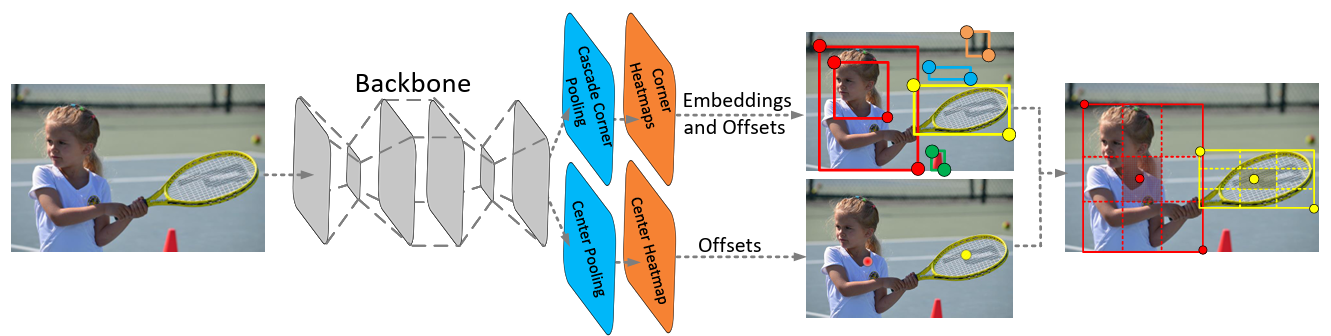
\includegraphics[width=1\columnwidth]{centernet.png}
\caption{CenterNet architecture. (Source: \cite{centernet})}
\label{fig:centernet}
\end{figure}

\section{Learning Using Privileged Information}
\label{subsec:2_lupi_background}

Unlike the conventional machine learning approach, which selects the most suitable function from a predefined set based solely on input-output training examples, the \gls{lupi} paradigm introduces a richer structure. Proposed by Vapnik and Vashist \cite{lupi, Vapnik2015LearningUP}, \gls{lupi} introduces an inherent asymmetry between training and inference: additional informative inputs, referred to as privileged information, are available during training but not at test time \cite{lab2wild, lupi_classification}. This distinction aims to accelerate the learning process by guiding the model with supplementary insights that cannot be exploited during deployment.

\gls{lupi} is inspired by human learning, reflecting the idea that a single day with a great teacher can be more valuable than a thousand days of independent study \cite{lupi_distillation, lupi}. Following the intuition that a student gains more than just examples, the teacher provides explanations, comparisons, and context, which enhance understanding \cite{lupi, lupi_distillation, lupi_nips}.
In much the same way, \gls{lupi} incorporates additional information, known as privileged information (\gls{x_star}), during training. This data, which is not available during testing, offers a deeper understanding beyond the standard input-output $($\gls{x}$ ,$ \gls{y}$)$ pairs. 
As outlined in \cite{lupi}, the standard supervised learning framework is formally expressed by a training set composed of input-output pairs:
\begin{equation} \label{eq:supervised_learning}
(x_1, y_1), \dots, (x_l, y_l), \quad x_i \in X, y_i \in Y  .
\end{equation}

\noindent Assuming that the data pairs $($\gls{x}$ ,$ \gls{y}$)$ are generated according to a fixed but unknown probability distribution \(P(x, y)\). The task is to select the function \(\hat{y} = f(x; \theta^{*})\), with parameter \(\theta^{*} \in \Theta\), from a specified class of functions which minimises the probability of misclassification. In this setting, the input vector \(x_i \in X\) describes an instance, and \(y_i\) denotes its corresponding target label. The predicted output \(\hat{y}\) is the model's estimate of the true label \(y\) given the input \(x\).
In comparison, within the \gls{lupi} framework, training data can be represented as a sequence of triplets:
\begin{equation} \label{eq:lupi_pairs}
(x_1, x_1^*, y_1), \dots, (x_l, x_l^*, y_l), \quad x_i \in X , x_i^* \in X^*, y_i \in Y .
\end{equation}

\noindent These samples are assumed to be drawn from an unknown but fixed probability distribution \( P(x, x^*, y) \). The task is to select, from a specified class of functions \( f(x, \theta) \), where \( \theta \in \Theta \), the function \( y = f(x, \theta^*) \) that minimises the probability of classification errors.
Although the aim remains the same as in the conventional supervised learning setting, the \gls{lupi} paradigm introduces an additional element during training. Rather than learning from pairs \( (x, y) \), the model receives triplets \( (x, x^*, y) \), where \( x^* \in X^* \) represents privileged information. This privileged component belongs to a separate space \( X^* \), which need not coincide with the original input space \( X \).

In addition, the \gls{lupi} framework can be extended to align with the concept of knowledge distillation \cite{hinton_distillation}, as proposed in \cite{lupi_distillation}. Both approaches can be viewed as instances of a broader idea in which one model provides guidance to another, a process referred to as \textit{generalised distillation}. This unified perspective treats Hinton’s distillation \cite{hinton_distillation} and Vapnik’s use of privileged information \cite{lupi} as complementary forms of machine-driven instruction.
In this framework, a teacher model is first trained on standard input-output $($\gls{x_star}$ ,$ \gls{y}$)$  pairs. The teacher then produces soft labels, which act as enriched supervisory signals. These soft labels are used in Hinton’s distillation method to train a student model. The student learns from the soft labels generated by the teacher, benefiting from the additional information embedded in the teacher’s predictions, even though it only receives standard input-output $($\gls{x}$ ,$ \gls{y}$)$  pairs \cite{lupi_distillation}.

Within practical implementations, \gls{lupi} in deep learning is generally realised through a teacher–student structure embedded in conventional training pipelines. The teacher network is trained using both regular inputs and privileged data. Its outputs, such as soft predictions or intermediate feature representations, are used to supervise the student through additional loss functions \cite{lupi_nips}. \gls{kl} divergence is often used for classification tasks, while cosine similarity is more suitable when aligning continuous outputs or internal vector representations \cite{lab2wild, hinton_distillation}. The architectures of the teacher and student are usually similar, though the teacher is adapted to accept the extra input during training \cite{lab2wild, lupi_distillation}. This setup integrates into existing deep learning workflows with minimal modification. Various strategies have been investigated for distilling knowledge, such as matching output logits \cite{output_logits}, aligning attention maps \cite{attention_maps_distillation}, transferring hidden features \cite{lab2wild, distillation2}, and combining multiple forms of guidance to strengthen the student’s learning process \cite{distillation1, lupi_distillation}. The application of \gls{lupi} within computer vision is examined in greater detail in Section~\ref{subsec:2_lupi}.

% -- Start of Lit Review --

\section{Review of Litter Detection Methodologies}
\label{sec:3_litter}

Within the broader context of object detection, the task of identifying litter poses particular challenges, especially when employing an \gls{uav} to capture expansive outdoor scenes. The difficulty lies in the nature of the environments: litter often appears amid textured and irregular backgrounds such as rocky outcrops or dense vegetation, where visual contrast is minimal \cite{small_litter_detection, taco2020, plastopol}. Despite these difficulties, several studies have addressed this problem by creating a dataset or proposing varied and increasingly refined approaches. In what follows, the review concentrates on the most prominent and widely cited works, offering a representative view of the prevailing methodologies adopted in recent research.

\subsection{Bottle Detection in the Wild Using Low-Altitude UAVs}
\label{subsec:3_bdw}

To address the challenge of bottle detection, the \gls{bdw} dataset, introduced in 2018, was developed to identify plastic bottles across varied environments using \gls{uav} imagery, with the broader aim of supporting recycling initiatives. The dataset comprises of images captured from a DJI Phantom 4 Pro quadcopter equipped with a 3-axis stabilised gimbal. The footage was taken at \gls{agl} altitudes ranging from 10 to 30 metres, with a resolution of $5472 \times 3078$ pixels. 
To bolster dataset diversity and simulate real-world conditions, the dataset includes images featuring eight distinct background types: bush forest land, step, flat land, sand land, wasteland, mixture, plastic stadium, and grassland, as illustrated in Figure \ref{fig:bdw}. This diversity of different backgrounds, presented as part of the dataset engineering process, accounts for the complexities associated with varied backgrounds in terms of generalising to real-world data. Furthermore, the authors highlight that the plastic bottles in the dataset are relatively small, with sizes less than $50 \times 50$ pixels, and are often transparent, which allows the background to be visible through the bottles, thereby significantly increasing the detection difficulty \cite{bdwdataset}.

\begin{figure}[!htbp]
    \centering
    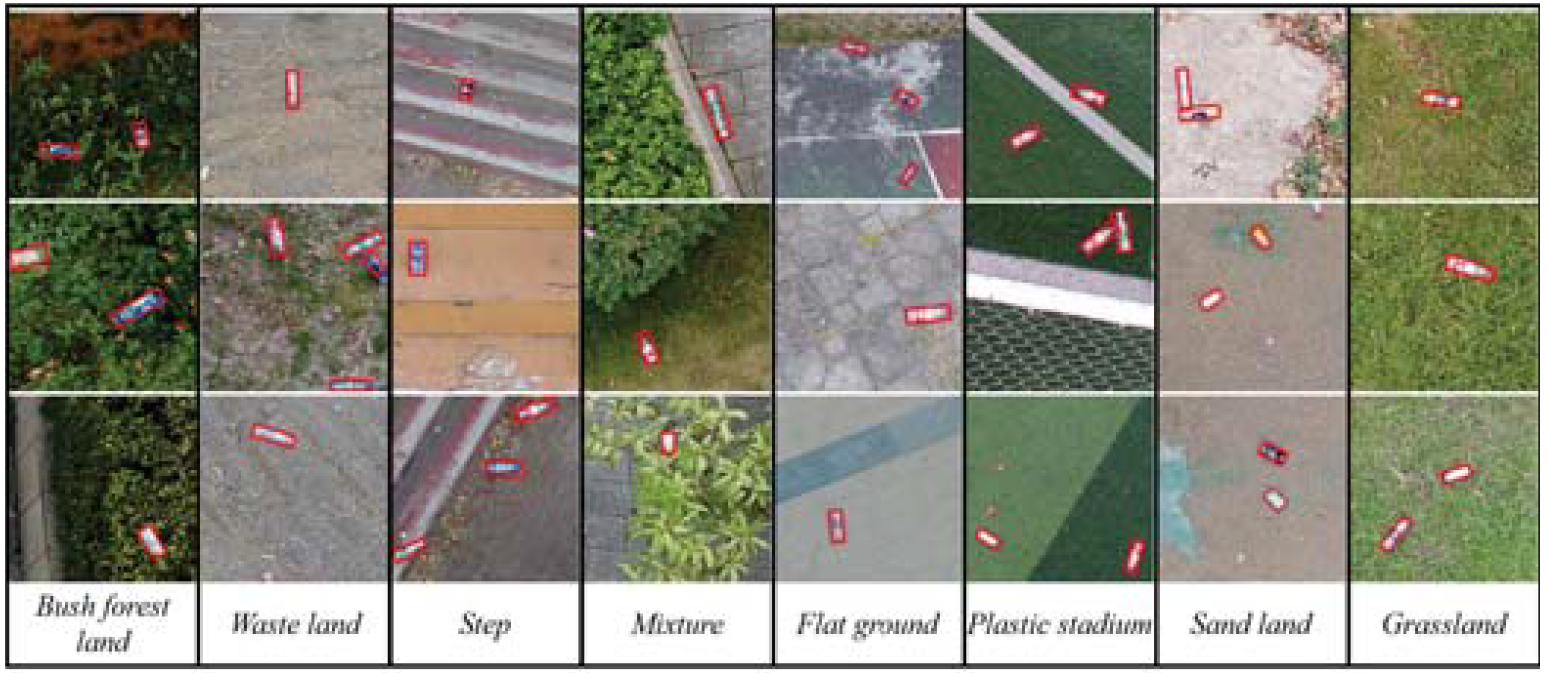
\includegraphics[width=0.9\linewidth]{BDWDataset1.png}
    \caption{Showcasing the different backgrounds found in the BDW dataset. (Source: \cite{bdwdataset})}
    \label{fig:bdw}
\end{figure}

The \gls{bdw} dataset contains 25,407 annotated images with 34,791 object instances, all belonging to a single category: \textit{plastic bottles}. Annotations in the \gls{bdw} dataset utilise \gls{obbs}, which include traditional bounding box coordinates along with additional parameters: centre coordinates ($c_x$, $c_y$), height ($h$), width ($w$), and orientation angle ($\theta$), where $\theta$ represents the angle from the horizontal axis. Additionally, the dataset was split randomly into training (64\%), validation (16\%), and testing (20\%) subsets \cite{bdwdataset}.

In their study, the authors utilise the created \gls{bdw} dataset in multiple experiments to train popular object detection models, including Faster \gls{rcnn}, \gls{ssd}, \gls{yolo}v2, and a Modified \gls{rrpn} from \cite{rrpn}. Among these models,  \gls{rrpn} uniquely predicts \gls{obbs}, whereas the others predict standard axis-aligned bounding boxes. Wang et al. report that these experiments demonstrate that OBB regression is crucial for oriented object detection. In addition,  \gls{rrpn} achieved superior localisation accuracy while minimising false alarms and false positives, making it the most robust model in the study \cite{bdwdataset}.

\subsection{Optimising Beached Litter Monitoring through Aerial Imagery}%UM Geo. Survey
\label{subsec:3_geosurvey}

Building on the concept of litter detection proposed by \cite{bdwdataset}, Deidun et al. (2018) introduced an optimised system for monitoring beach litter through aerial imagery \cite{umgeosurvey}. Their study focused on three coastal stretches within the North-East Marine Protected Area of the Maltese Islands. The monitored areas included Baħar iċ-Ċagħaq, specifically the western and eastern flanks of its rocky peninsula. 
The data collection process utilised a DJI Phantom 4 Pro drone, configured with a gimbal angle of -90 degrees and flown at an \gls{agl} altitude of 30 metres. This altitude was empirically determined to balance image quality and spatial resolution, following tests conducted at heights ranging from 20 to 50 metres. Images were captured at varying ground resolutions, ranging from 2.5 to 50 centimetres per pixel, to provide detailed visual data \cite{umgeosurvey}.

The collected footage was processed using OpenDroneMap software \cite{OpenDroneMap}, which facilitated the creation of point clouds and texture maps. Georeferenced orthophoto maps with a resolution of 1 centimetre per pixel were generated using \gls{gps} metadata embedded in the \gls{exif} data of each image file. These orthophotos were subsequently tiled and visualised in Google Earth \cite{umgeosurvey}.%©

\begin{figure}[!htbp]
    \centering
    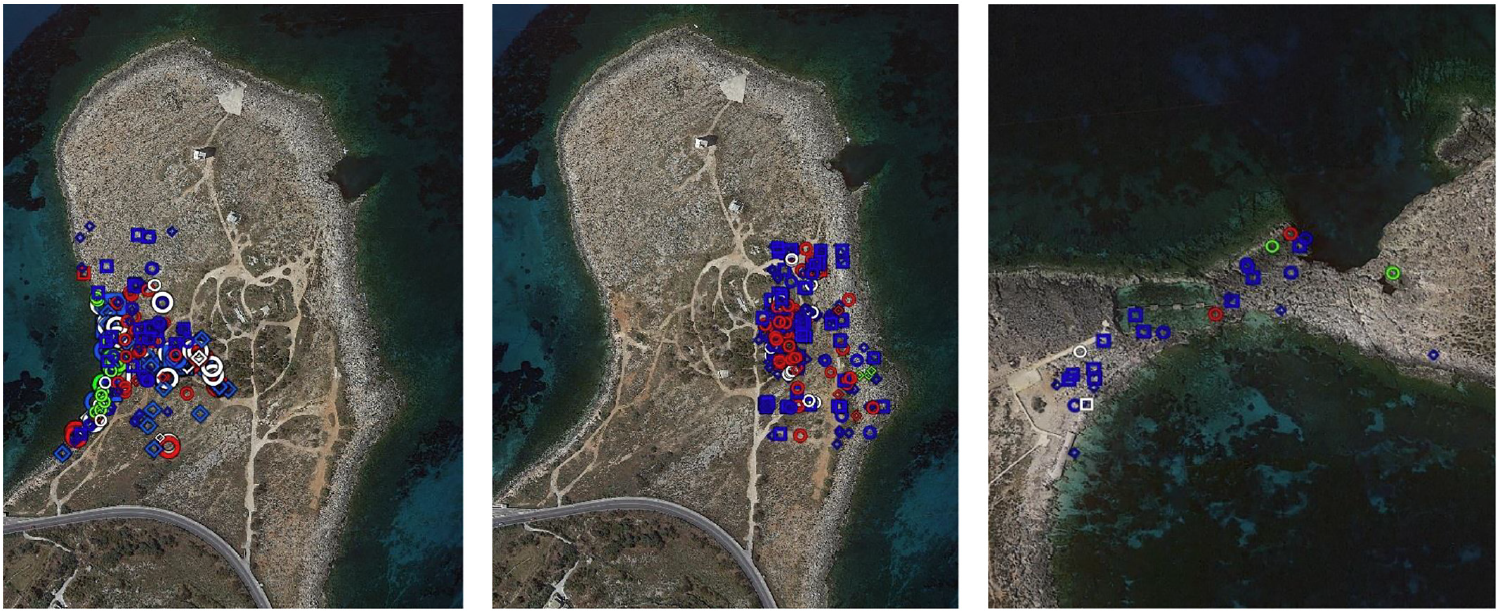
\includegraphics[width=1\linewidth]{UMgeosurvey.png}
    \caption{Showcasing snapshots from the digitised marine litter database, highlighting litter detected in the west (left) and east (middle) bays of Baħar iċ-Ċagħaq, and Qawra Point (right). Legend: blue = plastics; green = rope; red = wood; black = rubber; white = other non-natural materials. (Source: \cite{umgeosurvey})}
    \label{fig:geosurvey}
\end{figure}

The digitised database of detected marine litter, shown in Figure \ref{fig:geosurvey}, was created using 473 annotated images containing 608 labelled instances of litter. These instances were categorised into five litter types: \textit{plastics, rope, wood, rubber, and non-natural items}. While the study did not involve testing object detection algorithms, its key contribution lies in presenting a robust data collection protocol and improving problem understanding \cite{umgeosurvey}.

\subsection{SuperDock: Automated Floating Trash Monitoring System}
\label{subsec:3_superdock}

To address the environmental issue of trash in rivers, Niu et al. (2019) proposed an automated river trash monitoring system called SuperDock \cite{superdock}. This system consists of a \gls{rpu}, a docking station, and a \gls{uav}. SuperDock enables the \gls{uav} to land precisely on the docking station, where automated battery replacement is performed. This allows the \gls{uav} to resume its monitoring tasks without significant wasted time. SuperDock incorporates a deep learning-based trash detection module, leveraging the \gls{yolo}v3 architecture. As illustrated in Figure \ref{fig:superdock}, the system includes three key components: the \gls{rpu}, the docking station, and the \gls{uav}. The object detection process uses data collected from a consumer-grade \gls{uav} flying at an \gls{agl} altitude of 5 to 10 meters \cite{superdock}.

\begin{figure}[!htbp]
    \centering
    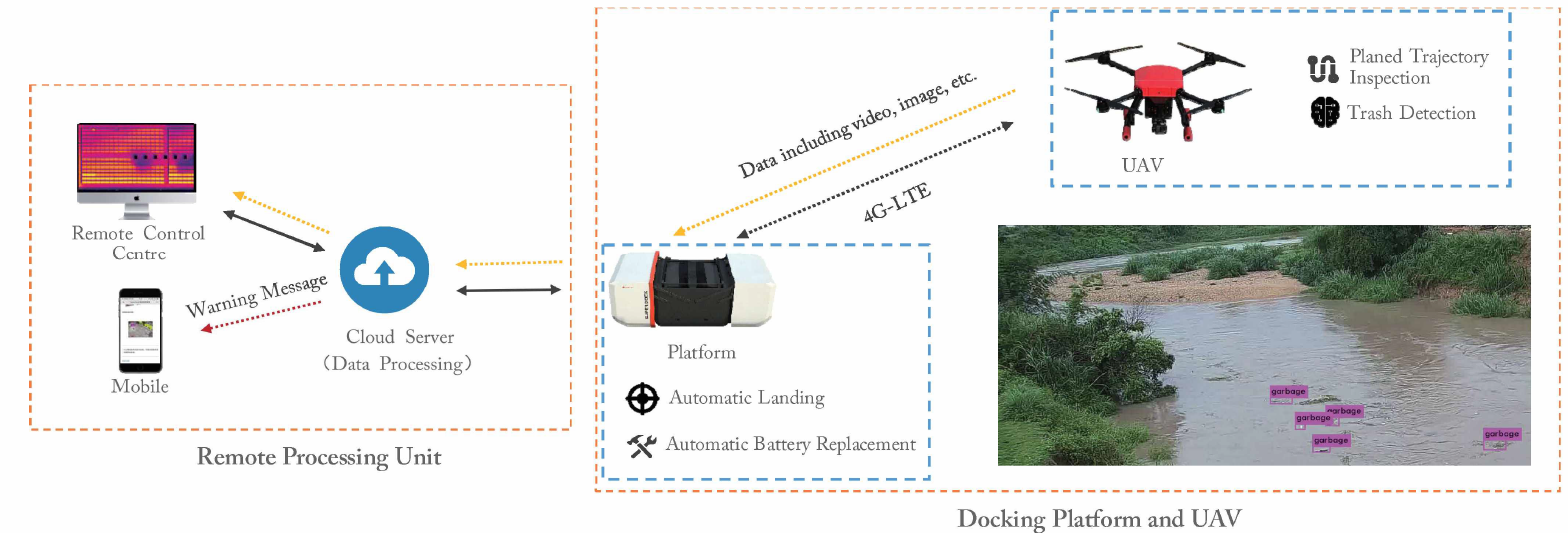
\includegraphics[width=0.9\linewidth]{superdock.png}
    \caption{Block diagram of the automated SuperDock system. (Source: \cite{superdock})}
    \label{fig:superdock}
\end{figure}

The dataset features 100 annotated images, divided into 80\% for training and 20\% for testing, with a total of 312 object instances. All types of litter in the dataset are annotated under a single category: \textit{garbage}. Data augmentation techniques were applied, increasing the dataset size by a factor of five. Additionally, the authors used Microsoft AirSim (Aerial Informatics and Robotics Simulation) to experiment with the gathered data. The dataset was used to train and test three object detection models: Faster \gls{rcnn}, \gls{yolo}v3, and \gls{yolo}v3 with an improved loss function. Among these, the improved \gls{yolo}v3 model demonstrated the best performance in terms of both accuracy and processing time. While the study did not focus on creating a specialised litter detection dataset, its primary contribution lies in developing an automated trash monitoring system \cite{superdock}.

\subsection{Detection and Monitoring of Styrofoam Litter using UAV Imagery}%Styrofoam Monitoring
\label{subsec:3_styrofoam}
To analyse the patterns of waste generation and distribution, as well as the factors contributing to its inflow, Bak et al. (2019) proposed an automated floating trash monitoring system based on deep learning \cite{styrofoam}. Their study focused on Heungnam Beach in Geoje, situated in Korea’s marine climate zone on the South Sea. The system utilises SegNet \cite{segnet}, an instance segmentation model based on a convolutional encoder-decoder structure developed by the University of Cambridge, to detect beach litter.
While the authors did not specify the exact number of annotated images in the dataset, \gls{uav} imagery was collected using DJI's MAVIC 2 PRO, a multi-rotor \gls{uav}. The \gls{uav} operated at an altitude of 15 meters, chosen to account for the size of the beach litter and the \gls{gsd}. Orthoimages were generated using Pix4D and divided into $224 \times 224$-pixel segments for neural network input, with positional information recorded for each segment \cite{styrofoam}.

\begin{figure}[!htbp]
    \centering
    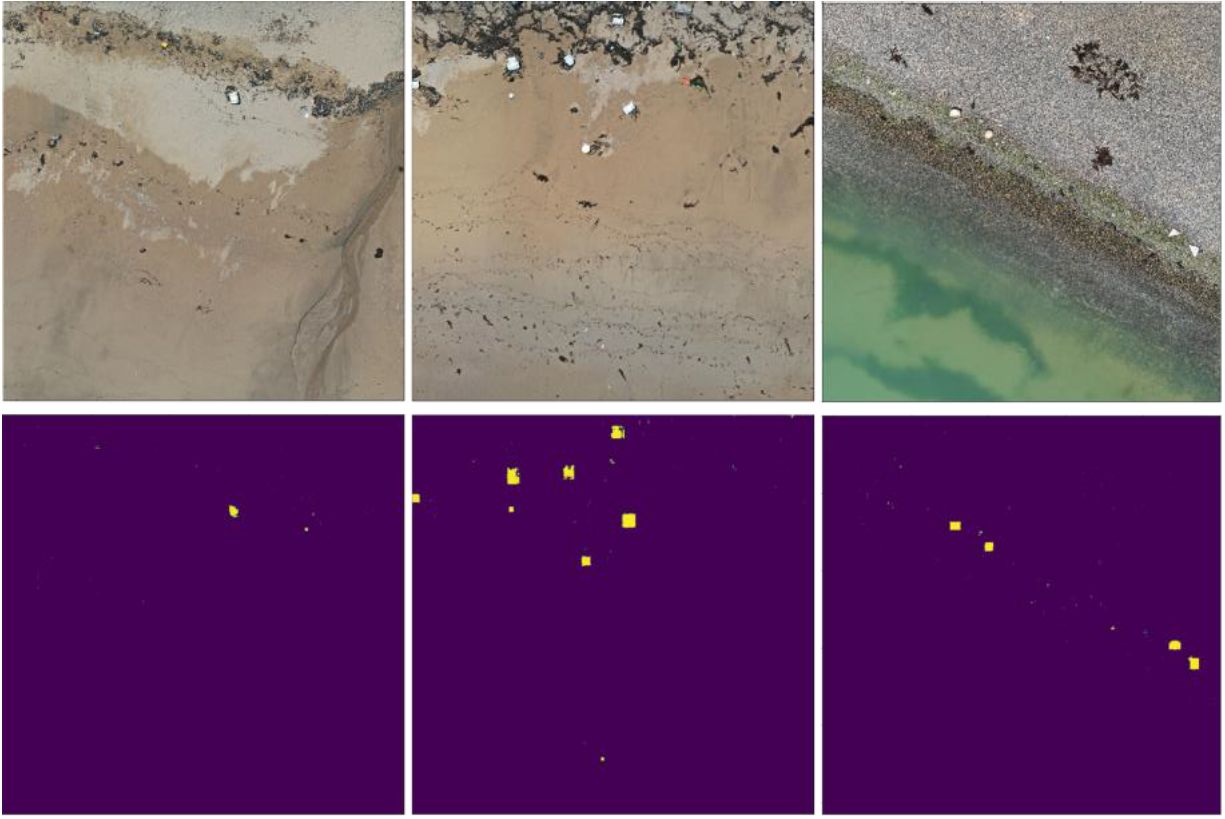
\includegraphics[width=0.8\linewidth]{styrofoam.png}
    \caption{Styrofoam detection results using the trained neural network. (Source: \cite{styrofoam})}
    \label{fig:styrofoam}
\end{figure}

The developed dataset only contained a single litter category, focusing on detecting \textit{Styrofoam} waste, and was notably imbalanced, as the majority of pixels represented the background, with less than 5\% occupied by detected objects. To mitigate this imbalance, data augmentation techniques were employed. Despite these challenges, the system achieved an impressive detection accuracy of 98.2\%, demonstrating its efficacy in identifying Styrofoam litter on beaches, as depicted in Figure \ref{fig:styrofoam} \cite{styrofoam}.

\subsection{Small Litter Detection in Highly Variable Backgrounds}
\label{subsec:3_smalldetection}

In 2019, Schembri and Seychell proposed a case study focusing on litter detection through aerial imagery to address challenges in small object detection in highly variable backgrounds \cite{small_litter_detection}. This study explored techniques for small object localisation using \gls{cnn} to detect litter in outdoor, non-urban imagery. The dataset for this research was collected using a consumer-grade \glspl{uav} at altitudes ranging from 5 to 10 metres \gls{agl}. Compiled from land surveys conducted within the Maltese Islands, the dataset includes 744 annotated images with all types of litter objects classified under a single \textit{litter} category \cite{small_litter_detection}.
The algorithmic pipeline proposed by the authors for small litter detection, is illustrated in Figure \ref{fig:smalllitterdetection}. A sliding window technique was used to subdivide the entire scene into tiles of $224 \times 224$ pixels with a 32-pixel overlap, and each tile was processed individually. Non-relevant objects such as the sky, sea, and humans were masked during a scene filtering stage to improve accuracy. The litter detection problem was tackled using a VGG-16 CNN model, pre-trained on ImageNet \cite{image_net}, and fine-tuned with the collected dataset. Data augmentation techniques were also applied to improve the model’s robustness \cite{small_litter_detection}.

\begin{figure}[!htbp]
    \centering
    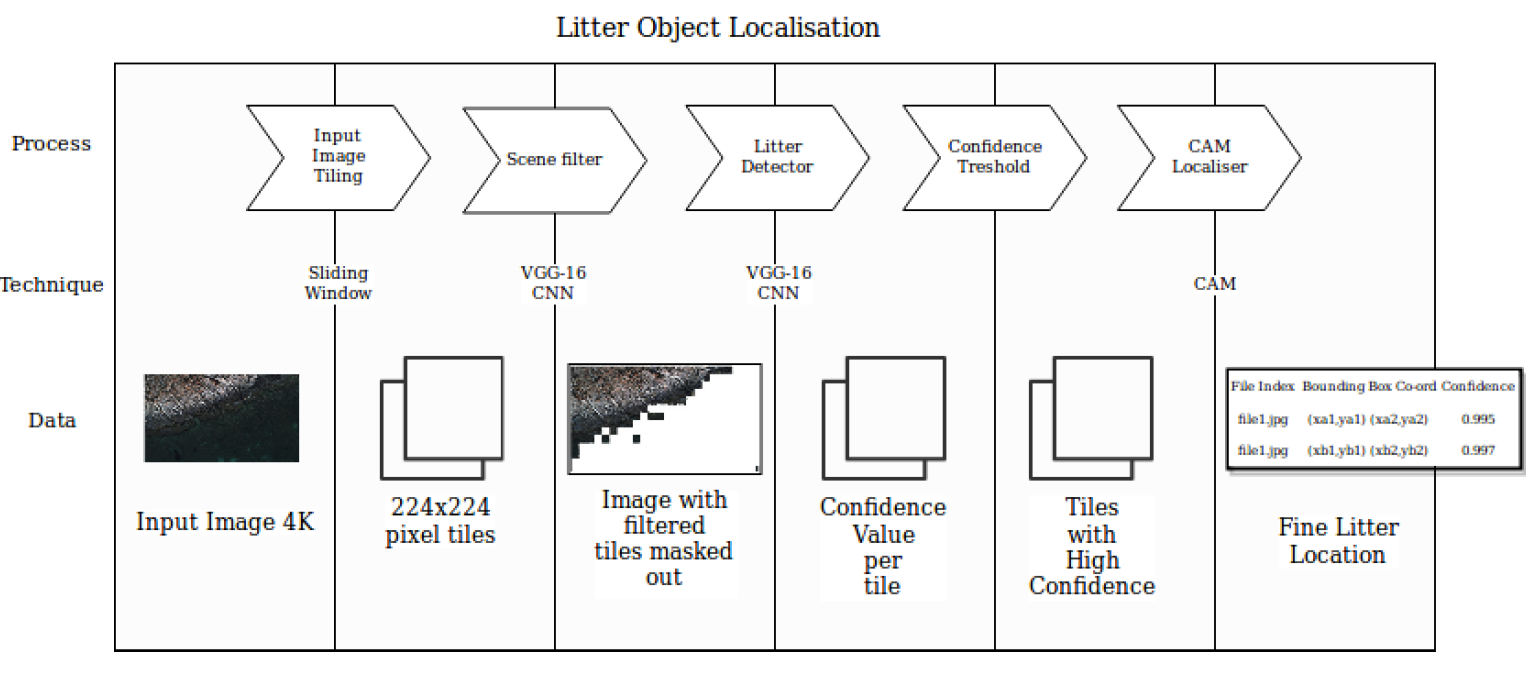
\includegraphics[width=0.9\linewidth]{small_litter_detection.png}
    \caption{Data flow and process diagram of the litter detection algorithm. (Source: \cite{small_litter_detection})}
    \label{fig:smalllitterdetection}
\end{figure}

Due to the dataset’s foreground-to-background sample ratio of 1:20, a confidence threshold was used to refine the detection results. \gls{cam} was employed to improve the \gls{iou} score by highlighting relevant foreground areas. Thresholding and normalising the heatmap allowed for generating masks that effectively located the target objects. An \gls{iou} threshold of 0.01 for \gls{nms} was used to facilitate the detection of very small objects.
Furthermore, the study identified that stones and vegetation were among the classes frequently misclassified as litter. To address this issue, the authors proposed a two-stage model incorporating a terrain filter to automate the detection of misclassifications, which provided improved results. They also concluded that litter with more defined shapes was easier to detect for both human annotation and algorithmic detection. 
Finally, the authors also trained the Faster \gls{rcnn} detection model on the same dataset and observed lower performance metrics, which were attributed to its inability in handling highly variable background representations \cite{small_litter_detection}.

\subsection{TACO: Trash Annotations in Context for Litter Detection}
\label{subsec:3_tacodataset}

Detecting litter in natural environments presents considerable challenges due to the variability of litter, which can be deformable, transparent, aged, fragmented, occluded, and camouflaged. Furthermore, models must contend with the wide variety of features found in natural landscapes. To tackle these issues, Proença and Simões introduced the \gls{taco} dataset in 2020 \cite{taco2020}. This dataset was created to feature images captured from a variety of global environments, as shown in Figure \ref{fig:taco1}, including beaches and urban areas, with litter segmented and annotated according to a hierarchical classification system \cite{taco2020}.

\begin{figure}[!htbp]
    \centering
    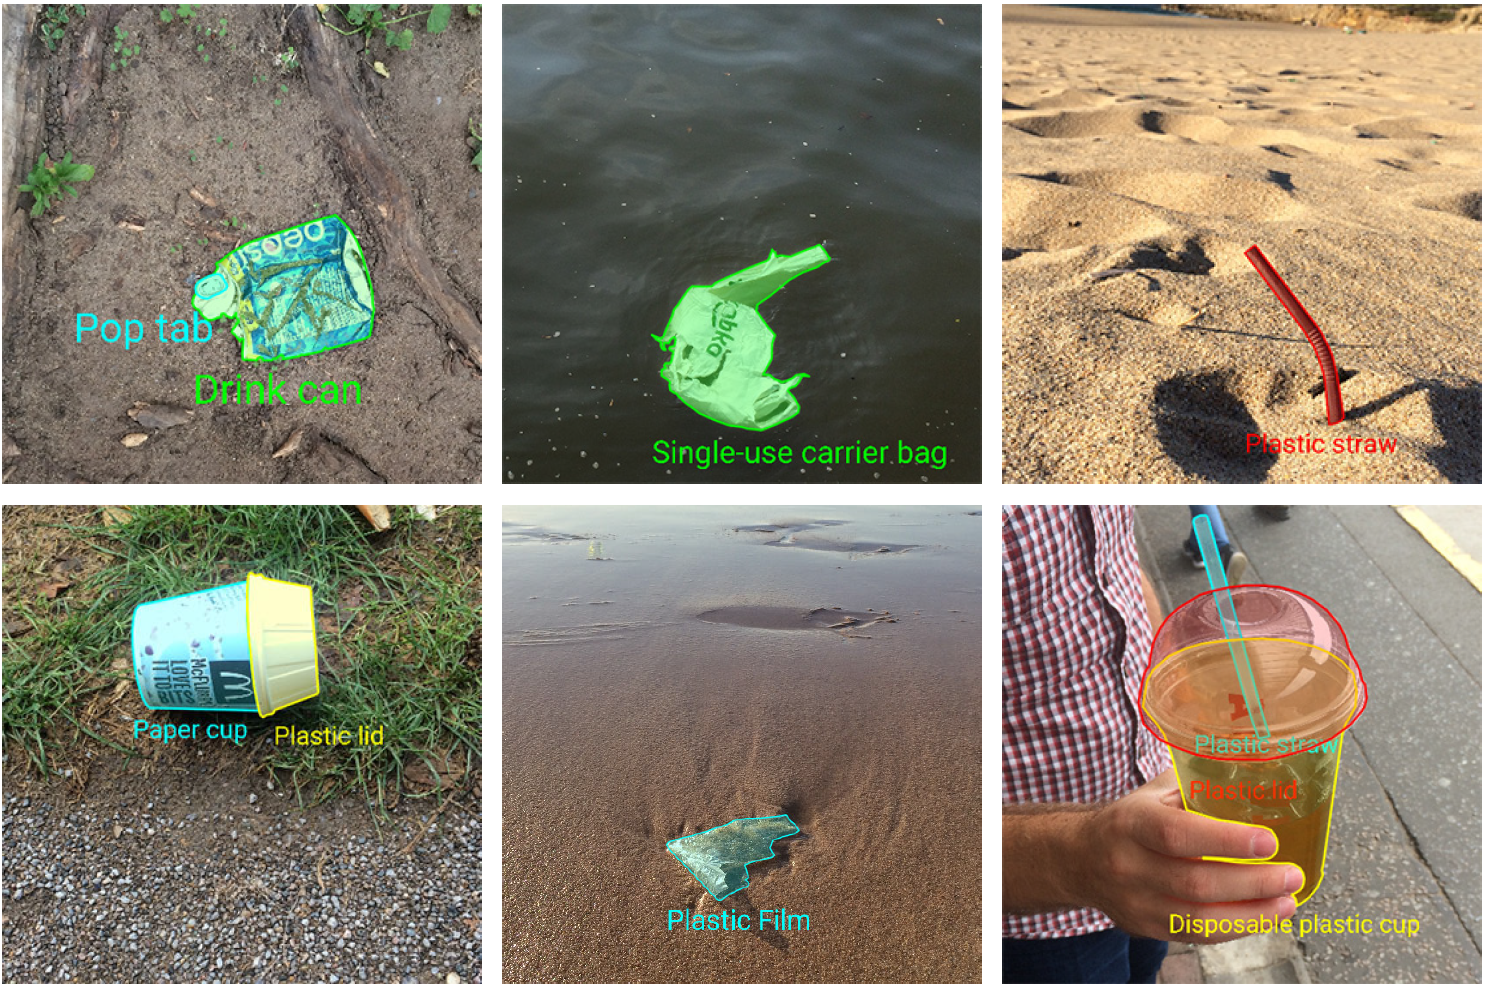
\includegraphics[width=0.8\linewidth]{taco1.png}
    \caption{Annotated images from the \gls{taco} dataset, with litter objects marked using polygon masks for instance segmentation. (Source: \cite{taco2020})}
    \label{fig:taco1}
\end{figure}

The \gls{taco} dataset includes 60 distinct litter categories, organised into 28 top-level (super) categories, as observed in Figure \ref{fig:taco2}. Unlike \gls{uav}-based datasets, \gls{taco} consists of images captured from ground-level natural environments. At the time of release, the dataset comprised 1,500 annotated images and 4,784 instances of litter, with an additional 3,918 new images currently awaiting annotation. The dataset uses polygon masks for annotation in an attempt to tackle the problem of both object detection, and instance segmentation \cite{taco2020}.
The authors conducted several experiments using Mask \gls{rcnn} to evaluate the dataset's performance. Two configurations were tested:
\begin{itemize}
    \item \textbf{\gls{taco}-1:} Identifying a single class of litter.
    \item \textbf{\gls{taco}-10:} Identifying ten distinct litter classes.
\end{itemize}

\begin{figure}[ht]
    \centering
    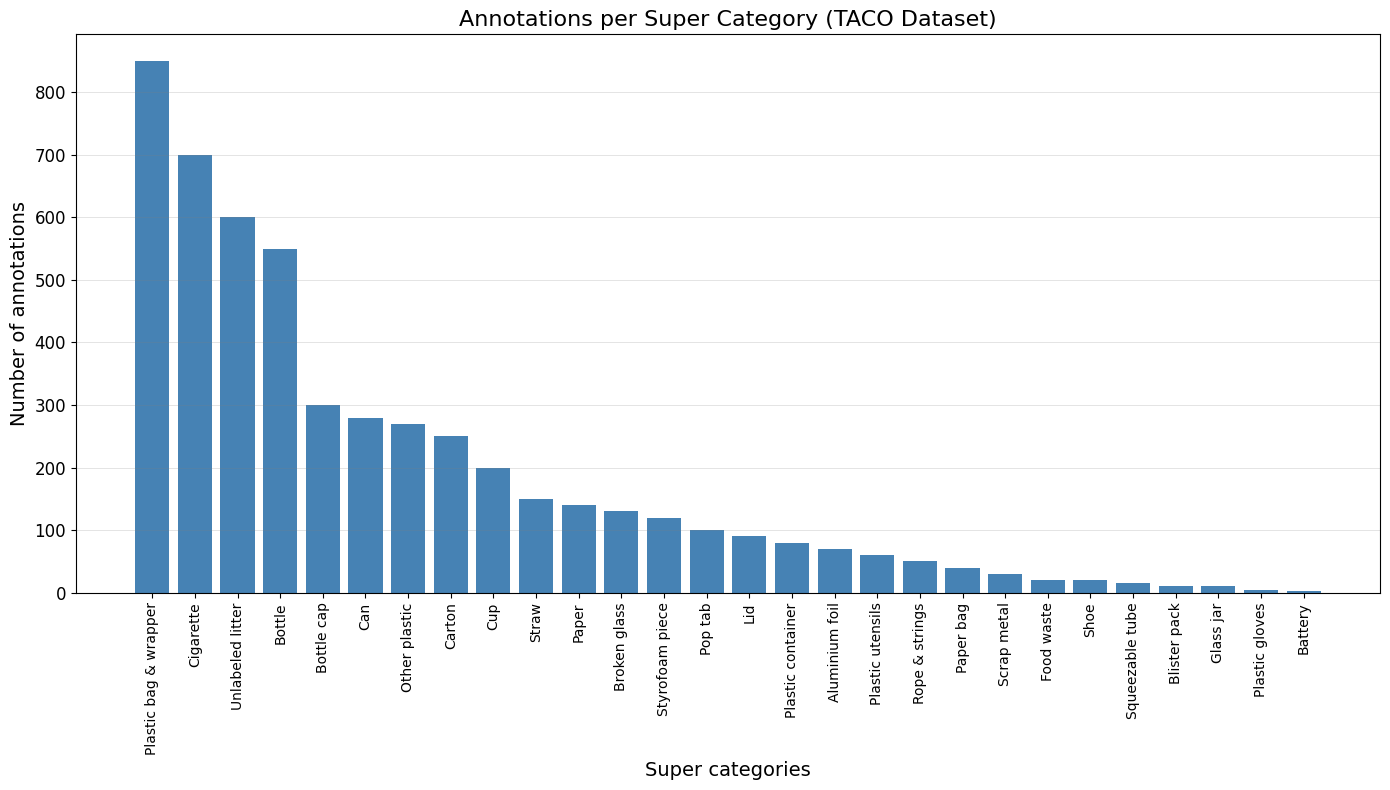
\includegraphics[width=1\linewidth]{taco2.png}
    \caption{Number of annotations per super category in the published version of the \gls{taco} dataset. (Source: \cite{taco2020})}
    \label{fig:taco2}
\end{figure}

The authors noted that the detection performance was notably low due to challenges in detecting small items, particularly cigarette butts, which led to a high rate of false positives and negatives. This was attributed to their small size, with most images resized to $1024 \times 1024$ pixels, causing many small objects (less than $20 \times 20$ pixels) to be missed. Larger objects, such as cans and bottles, were detected more accurately, though a considerable number of bottles were misclassified as cans. Confusion was also observed between \textit{plastic bags} and \textit{other litter}, which is understandable given the material similarities between these categories \cite{taco2020}.

\subsection{Multi-Level Approach to Waste Object Segmentation}
\label{subsec:3_mju-waste}

In 2020, Wang et al. also sought to address the challenge of waste object segmentation through a multi-level approach \cite{mju_waste}. To create their dataset, the authors collected waste items from a university campus, photographed individuals holding these items, and then annotated the images. The MJU-Waste dataset focuses solely on a single category, classifying all items under the label of \textit{waste}. The MJU-Waste dataset contains 2,475 annotated images and 2,525 instances of litter, all of which are annotated using polygon masks.
Unlike \gls{uav}-based datasets, the MJU-Waste dataset consists of images captured from controlled environments. The dataset includes segmentation masks, along with both raw and processed depth maps for all litter instances, captured using a Microsoft Kinect \gls{rgbd} camera. However, due to sensor limitations, the depth frames contain missing values, notably at reflective surfaces, occlusion boundaries, and distant regions. To address this, a median filter was applied to fill in the missing data and ensure the depth images were of high quality. Each image in the dataset was annotated with pixel-wise masks of the waste objects, and examples of colour frames, ground-truth annotations, and depth frames are provided in Figure \ref{fig:mjuwaste}. Alongside the semantic segmentation ground truths, object instance masks are also available \cite{mju_waste}.

\begin{figure}[!htbp]
    \centering
    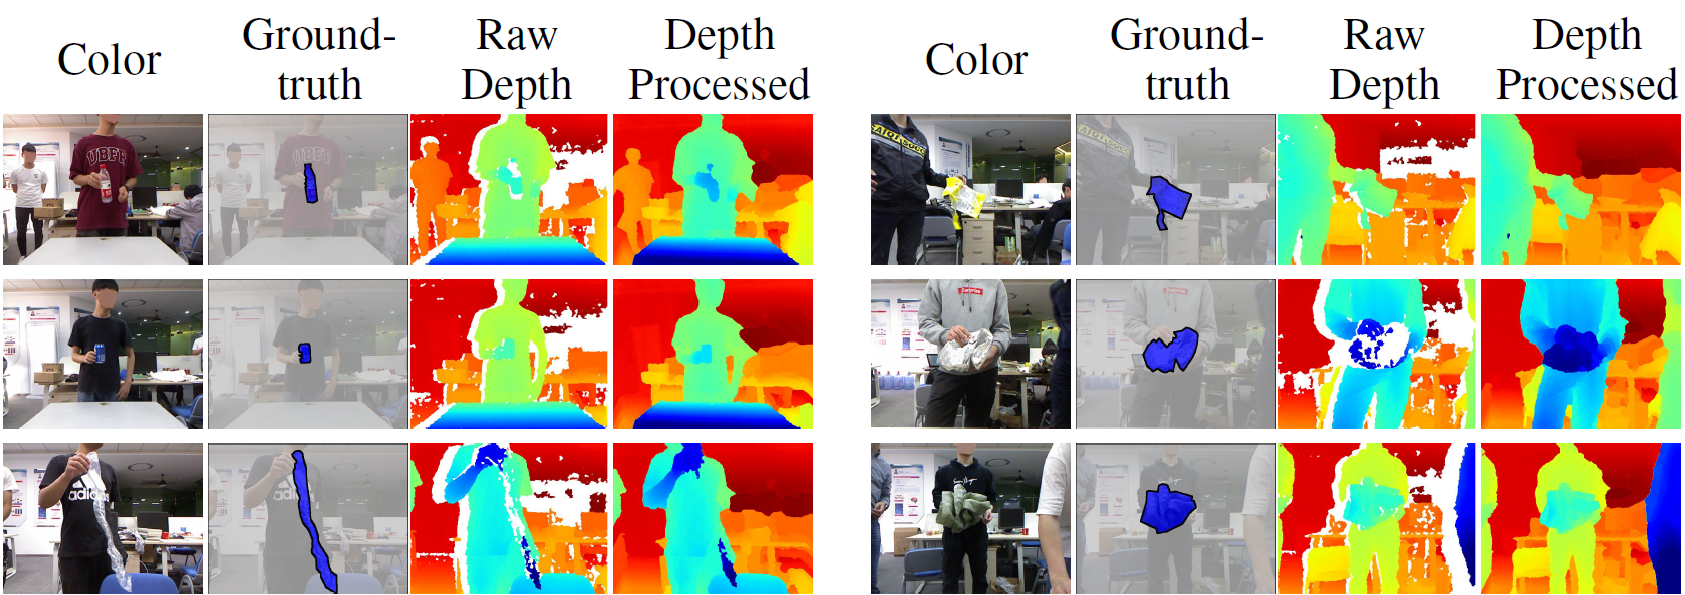
\includegraphics[width=1\linewidth]{mjuwaste.png}
    \caption{Sample RGB images, ground-truth annotations, and depth frames from the MJU-Waste dataset. (Source: \cite{mju_waste})}
    \label{fig:mjuwaste}
\end{figure}

The authors evaluate their proposed method against state-of-the-art semantic segmentation baselines. Their approach adopts a multi-level strategy for waste object segmentation, involving three key stages: first, scene-level parsing for initial coarse segmentation; second, object-level parsing to refine object region proposals; and third, pixel-level refinement using colour, depth, and spatial affinities. By combining inference from all three levels, the method achieves a coherent and accurate final segmentation.
In addition, the study focuses on two particularly challenging scenarios for waste object localisation: the hand-held setting, which is crucial for applications such as service robot interactions and smart trash bins, and waste objects found in natural environments. A significant challenge noted by the authors in both cases is the extreme variation in object scale, which leads to suboptimal performance from standard segmentation algorithms \cite{mju_waste}.
In comparison to the \gls{taco} dataset, the MJU-Waste dataset is split as follows: 60\% for training, 10\% for validation, and 30\% for testing. The evaluation metrics used include \gls{iou}, mean \gls{iou}, and pixel precision. The models tested include FCN-8s \cite{fcn}, PSPNet \cite{pspnet}, CCNet \cite{ccnet}, and DeepLabv3 \cite{deeplabv3}. Among these, DeepLabv3 performed best in terms of \gls{iou} and mIoU, while CCNet excelled in pixel precision. Notably, DeepLabv3 also outperformed other models when tested on the \gls{taco} dataset.
The authors also conclude that their multi-level approach proved effective, with scene-level segmentation, object-level segmentation, and pixel-level refinement working together to produce high-quality localisation results \cite{mju_waste}.

\subsection{UAVVaste: Vision-Based Trash and Litter Detection in Low Altitude Aerial Images}
\label{subsec:3_uavvaste}

In 2021, Kraft et al. addressed the challenge of detecting litter and the associated issue of mapping detected litter geographically \cite{uavvaste}. Their proposed system employed a \gls{uav} equipped with onboard sensors to process low-altitude aerial imagery. A key feature of the system was its reliance on low-cost, commercially available components, which were integrated into a self-contained solution capable of autonomous operation during \gls{uav} patrol missions.
A notable contribution of their research was the introduction of an application-specific dataset, UAVVaste. This dataset consists of 772 images with 3,716 bounding box annotations, as illustrated in Figure \ref{fig:uavvaste1}, and is dedicated to a single category: litter, labelled as \textit{rubbish}. The creation of this dataset was motivated by the lack of domain-specific data tailored to \gls{uav}-based litter detection. Compared to the \gls{taco} dataset, the UAVVaste dataset features a marked distribution shift, characterised by smaller object sizes, reflecting the unique challenges of detecting litter in aerial imagery \cite{uavvaste}.

\begin{figure}[!htbp]
    \centering
    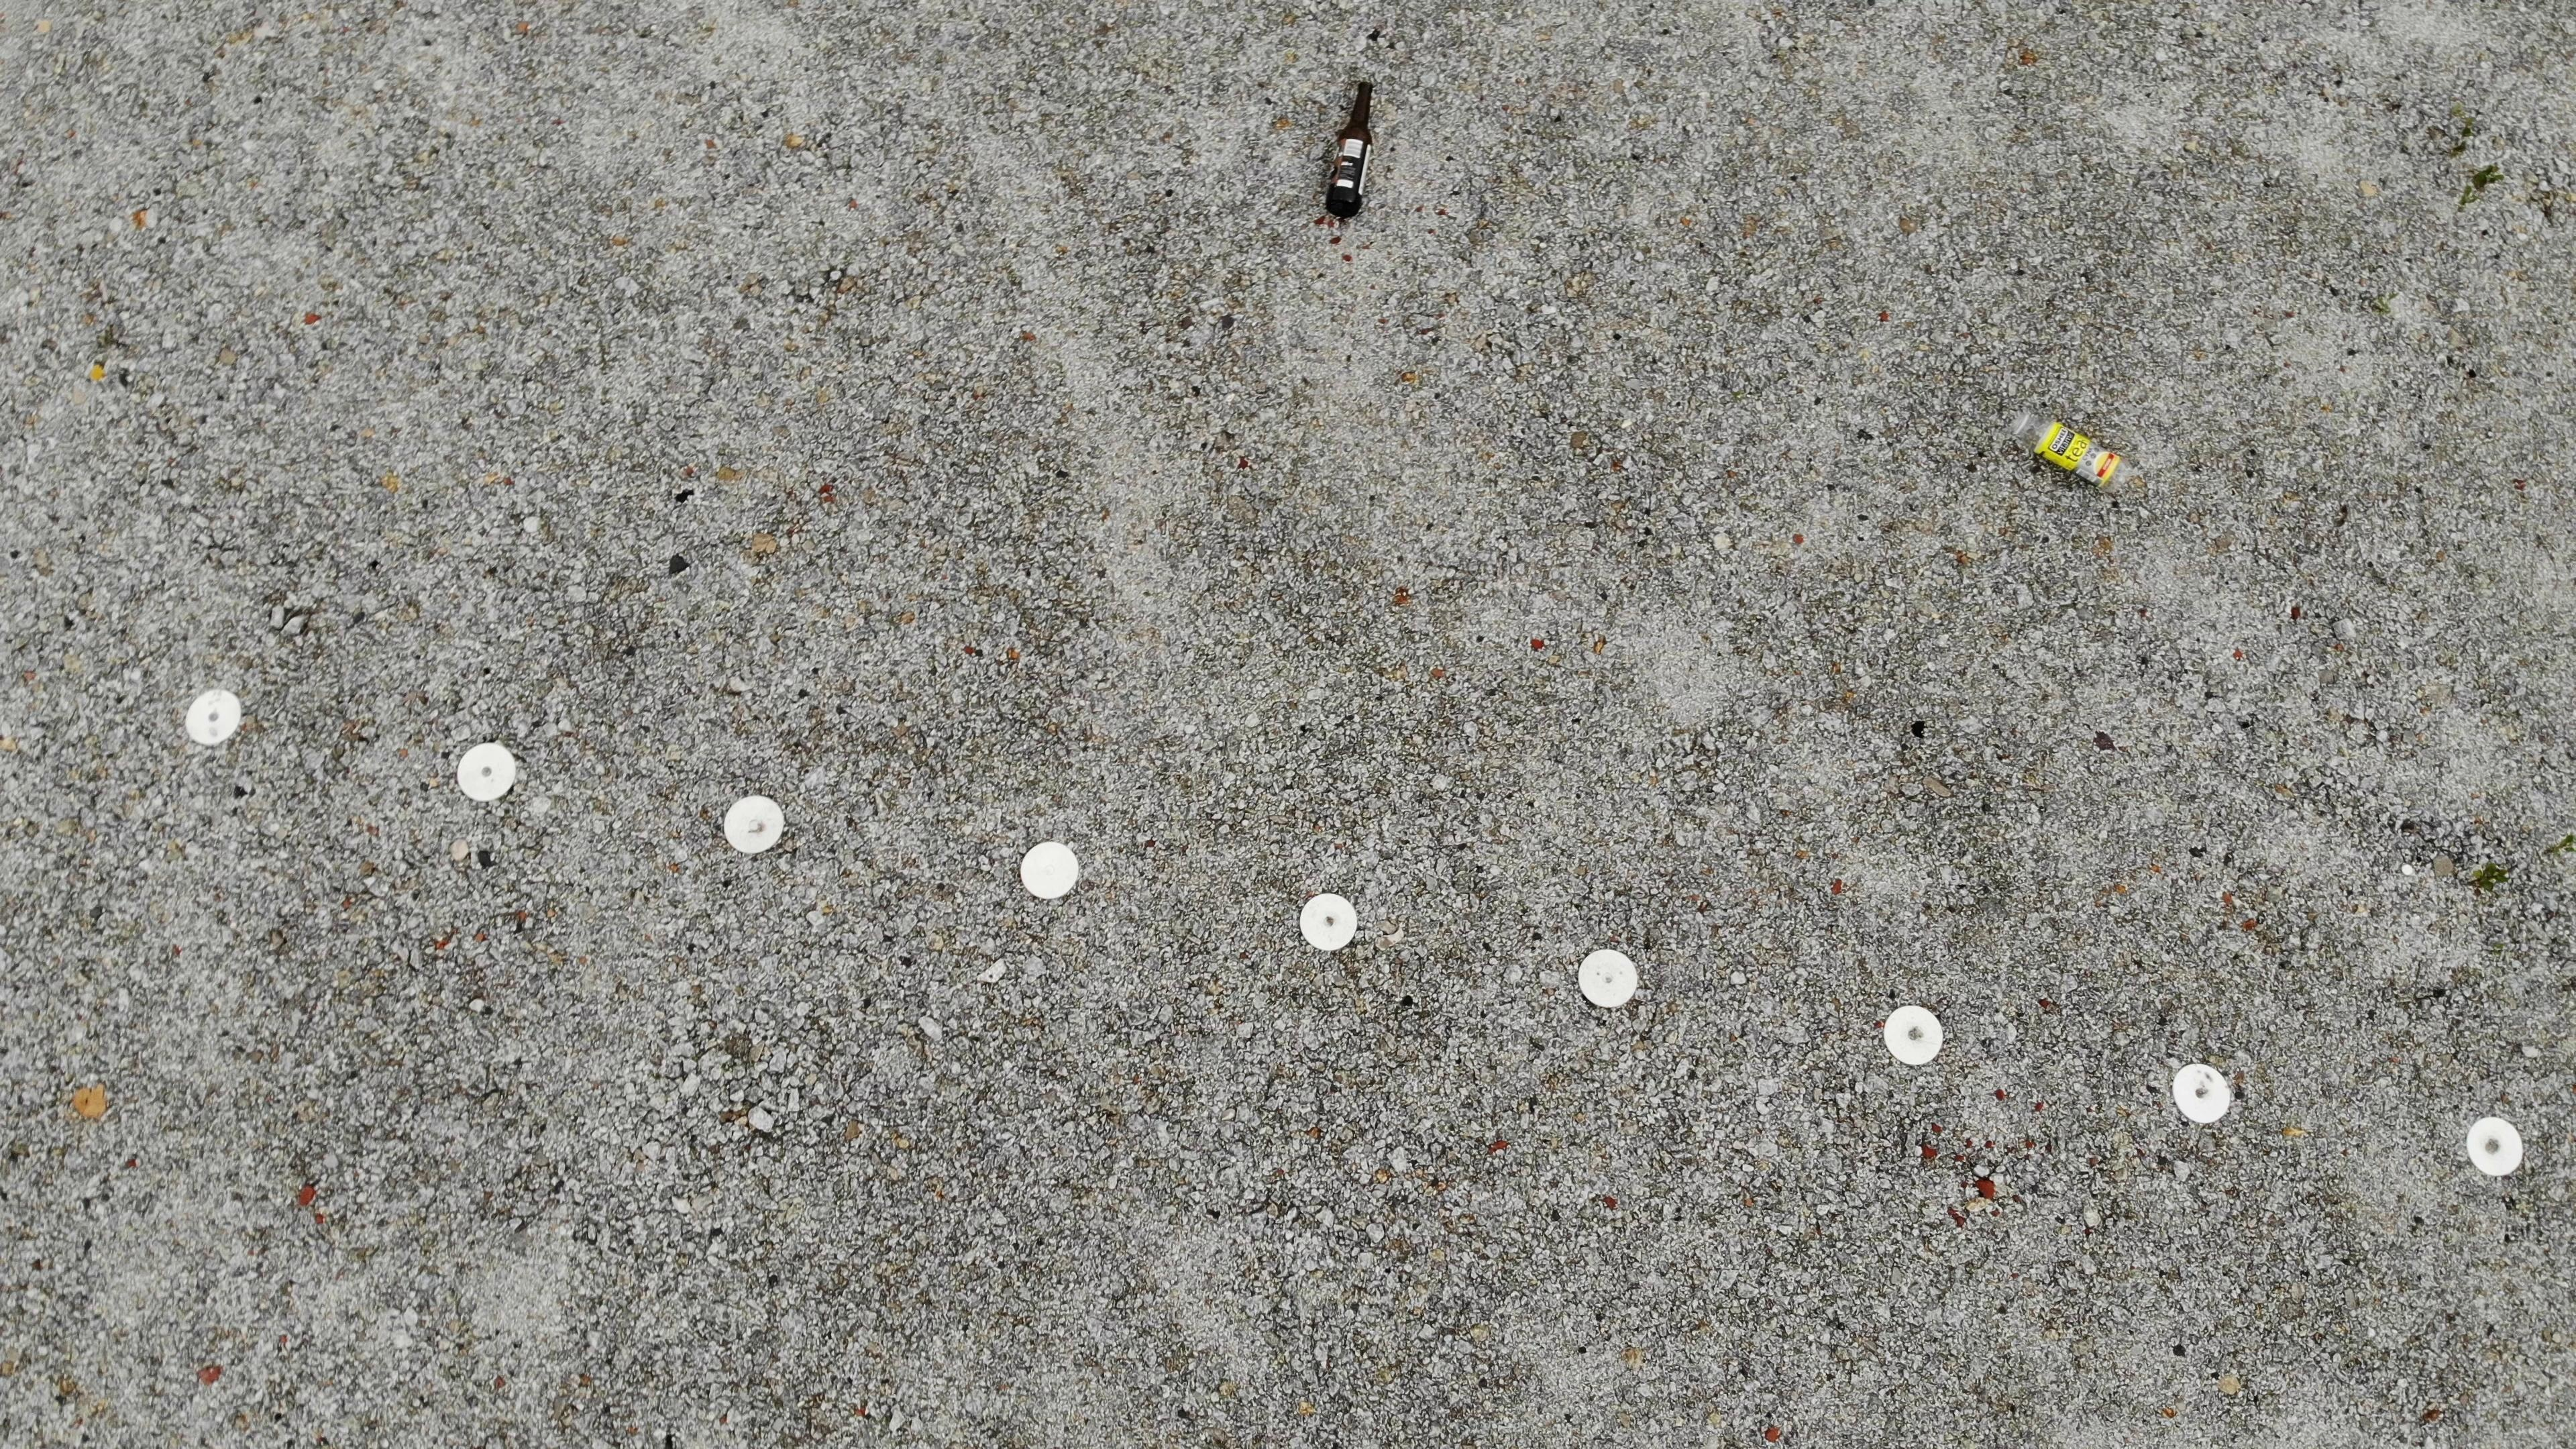
\includegraphics[width=0.9\linewidth]{uavvaste1.png}
    \caption{Sample images from the UAVVaste dataset with litter objects annotated using bounding boxes. (Source: \cite{uavvaste})}
    \label{fig:uavvaste1}
\end{figure}

The \gls{uav} hardware used in the study included a Pixhawk 2 autopilot controller, a Here2 \gls{gps}/\gls{gnss} module equipped with a barometric pressure sensor, and a downward-facing camera stabilised using a gimbal. The computational platform featured multiple components, including an Nvidia Xavier NX, a Google Coral USB (\gls{tpu}), and a Raspberry Pi 4. A variety of neural network architectures were evaluated for litter detection. These included \gls{ssd} detectors with lightweight backends optimised for TensorFlow Lite, which operated efficiently on the Google Coral \gls{tpu}, as well as \gls{yolo}v3 and \gls{yolo}v4 and their lightweight variants. For models deployed on the Nvidia Xavier NX, TensorRT was utilised to optimise performance. Additionally, EfficientDet with a MobileNet backend was implemented. Training these models involved transfer learning, leveraging pre-trained weights from the \gls{coco} dataset to improve performance \cite{uavvaste}.

% \begin{figure}[!htbp]
%     \centering
%     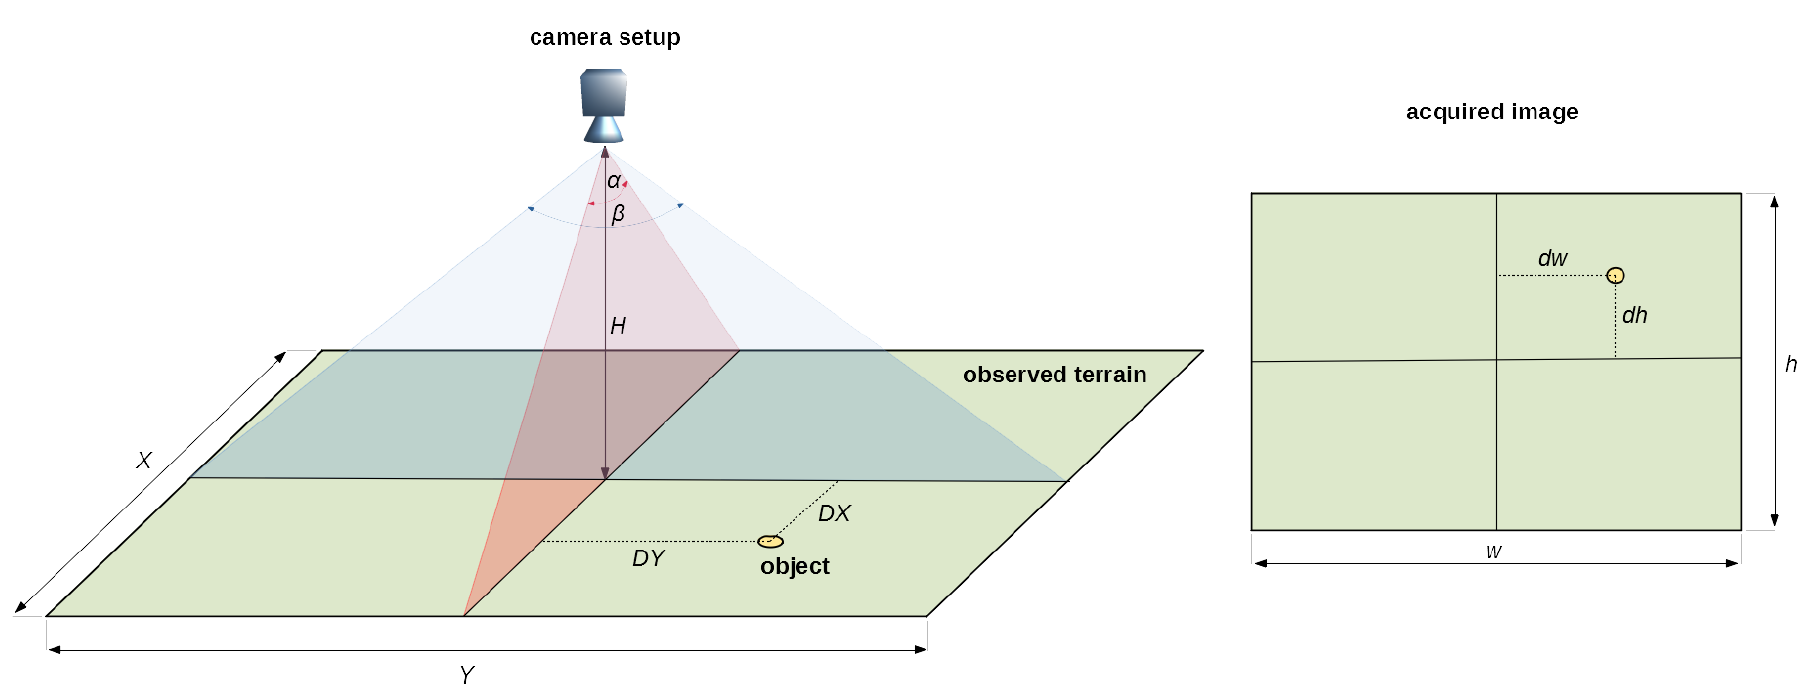
\includegraphics[width=0.9\linewidth]{uavvaste2.png}
%     \caption{A schematic representation of the camera setup and acquired image, along with the key parameters. (Source: \cite{uavvaste})}
%     \label{fig:uavvaste2}
% \end{figure}

% A significant portion of the study focused on creating a geolocation algorithm, which marks detected litter objects on a map using the UAV’s onboard sensors. This process required camera calibration, performed using the Kalibr library, and lens distortion correction, ensuring accurate geometric relationships between the image and real-world coordinates. The algorithm assumed a vertical downward orientation for the camera during operation. Using the known viewing angles of the camera and the UAV’s altitude, the algorithm calculated the size of the area captured in each image. Figure \ref{fig:uavvaste2} provides a schematic representation of the camera setup and the acquired image, highlighting the key parameters involved in the process. While the camera parameters were determined with high precision, the accuracy of object localisation on the map was predominantly influenced by the accuracy of altitude measurements. The authors observed that any error in altitude measurement would proportionally affect the localisation accuracy.
A significant portion of this study also involved developing a geolocation algorithm to map detected litter using \gls{uav} sensor data. Camera calibration and distortion correction were performed to ensure accurate mapping, assuming the camera faced directly downward. The algorithm used the \gls{uav}'s altitude and camera angles to estimate ground coverage, with localisation accuracy largely dependent on altitude measurement precision.
Alongside this spatial mapping component, model performance was evaluated using standard detection metrics. The evaluation included the \gls{map} scores from the \gls{coco} dataset, calculated at \gls{iou} thresholds of 0.5 and 0.95. Separate \gls{map} and recall scores were also reported for small, medium, and large objects. Among the models tested, \gls{yolo}v4 achieved the highest \gls{map}, while EfficientDet excelled in recall, particularly for smaller objects \cite{uavvaste}.

\subsection{ZeroWaste: Towards Automated Waste Recycling}
\label{subsec:3_zerowaste}

In 2022, Bashkirova et al. introduced the first industrial-grade, in-the-wild waste detection and segmentation dataset, ZeroWaste, making a significant contribution to computer-aided waste detection \cite{zerowaste}. The dataset features four categories of litter: \textit{cardboard}, \textit{soft plastic}, \textit{rigid plastic}, and \textit{metal}. Unlike \gls{uav}-based datasets, the images in ZeroWaste were captured in real-world settings.
The ZeroWaste dataset includes 10,715 annotated images, collected from a high-quality paper conveyor at a single-stream recycling facility in Massachusetts, containing 27,744 instances of litter, all annotated in polygon format, as illustrated in Figure \ref{fig:zerowaste}. Data augmentation was also applied to the dataset to improve model generalisation by artificially increasing the variety of training samples. Furthermore, this four-class labelled dataset captures various waste items identified during the sorting process at the facility, which aims to separate high-quality paper from contaminants such as metal, plastic, brown paper, and cardboard \cite{zerowaste}.

\begin{figure}[!htbp]
    \centering
    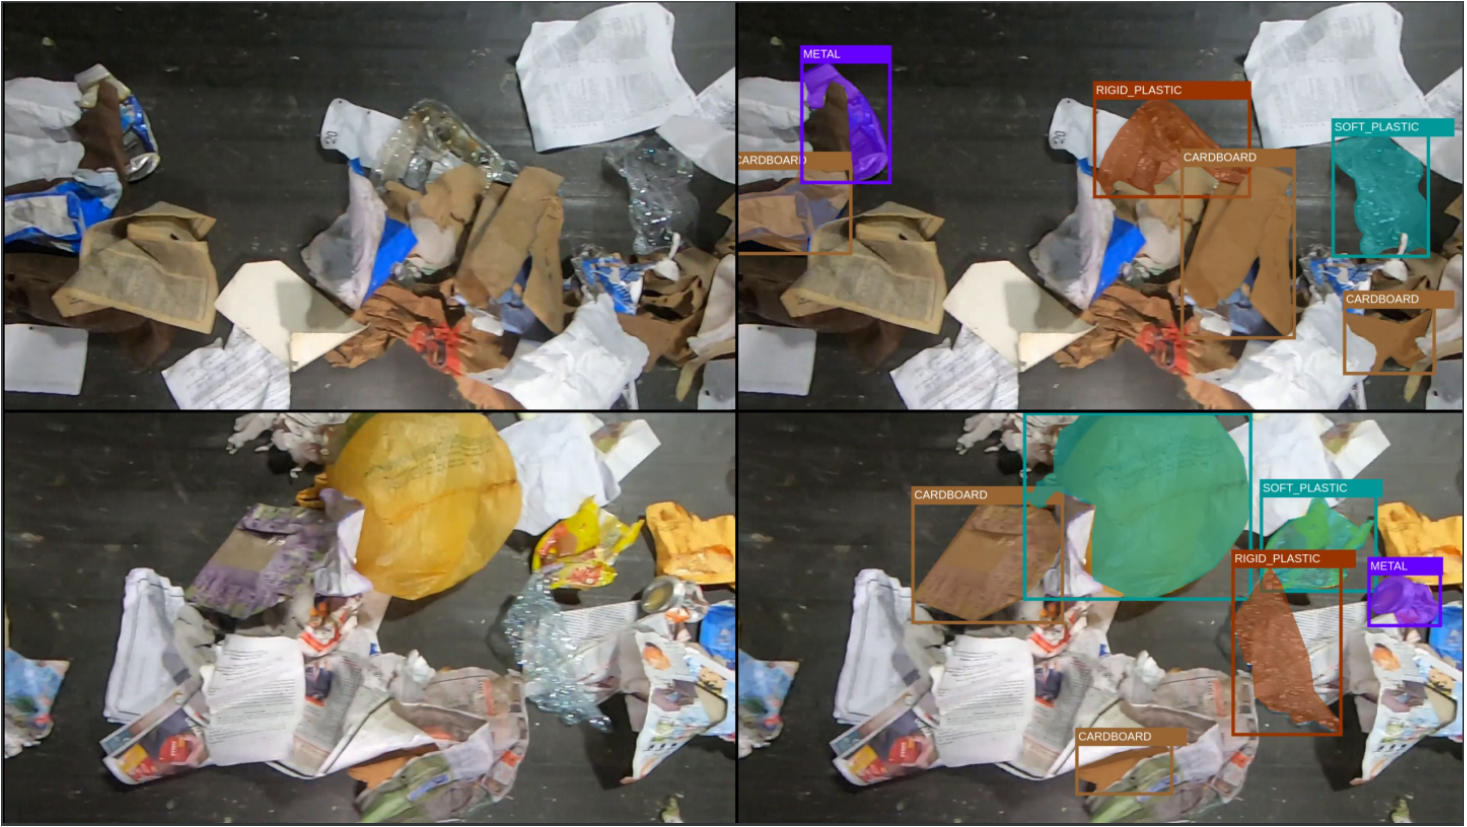
\includegraphics[width=0.9\linewidth]{zerowaste.png}
    \caption{Sample images (left) and ground truth polygon annotations (right) in the ZeroWaste dataset. (Source: \cite{zerowaste})}
    \label{fig:zerowaste}
\end{figure}

The data was gathered using two compact recording systems placed at the start and end of the conveyor belt during the facility's routine operations. The footage consists of 12 video sequences with a total duration of 95 minutes and 14 seconds, recorded at a frame rate of 120 \gls{fps} and a resolution of $1920 \times 1080$. To ensure high-quality data, the footage was processed to correct optical distortions, crop unnecessary elements, and remove motion blur.
The ZeroWaste dataset was divided as follows: 65\% for training, 15\% for validation, and 20\% for testing. The evaluation metrics used include \gls{ap} and \gls{map} at various thresholds, \gls{iou}, and pixel precision. Additionally, the models tested include RetinaNet, Mask \gls{rcnn}, TridentNet \cite{tridentnet}, and DeepLabv3, and a series of experiments were conducted, including fully, semi, and weakly supervised learning.
The results revealed that the ZeroWaste dataset posed considerable challenges for state-of-the-art detectors such as Mask \gls{rcnn}. However, TridentNet emerged as the top-performing detector, while DeepLabv3 achieved the best results in terms of segmentation \cite{zerowaste}.

\subsection{PlastOPol: Litter Detection with Deep Learning}
\label{subsec:3_plastopol}

To address the issue of litter accumulation, Córdova et al. investigated the efficacy of lightweight neural networks for detecting litter in real-world environments with complex and crowded image backgrounds \cite{plastopol}. The study also evaluated the feasibility of deploying these models on mobile devices with limited memory capacity. Their 2022 publication presented two key contributions: a comparative analysis of state-of-the-art deep learning techniques for image-based litter and waste detection and the introduction of a novel dataset, PlastOPol, comprising 2,418 images captured in real-world conditions with 5,300 litter annotations.
The PlastOPol dataset includes a single class, with all litter items categorised under the label \textit{litter}. The dataset consists of images from natural settings rather than being derived from \gls{uav} data. These images were sourced using the Marine Debris Tracker and are publicly available under a Creative Commons Attribution licence. The dataset was annotated in a bounding box format and focused on the problem of object detection. Of the 5,300 annotated instances, 90.98\% are large objects, 8.40\% are medium objects, and only 0.62\% are small objects \cite{plastopol}.

\begin{figure}[!htbp]
    \centering
    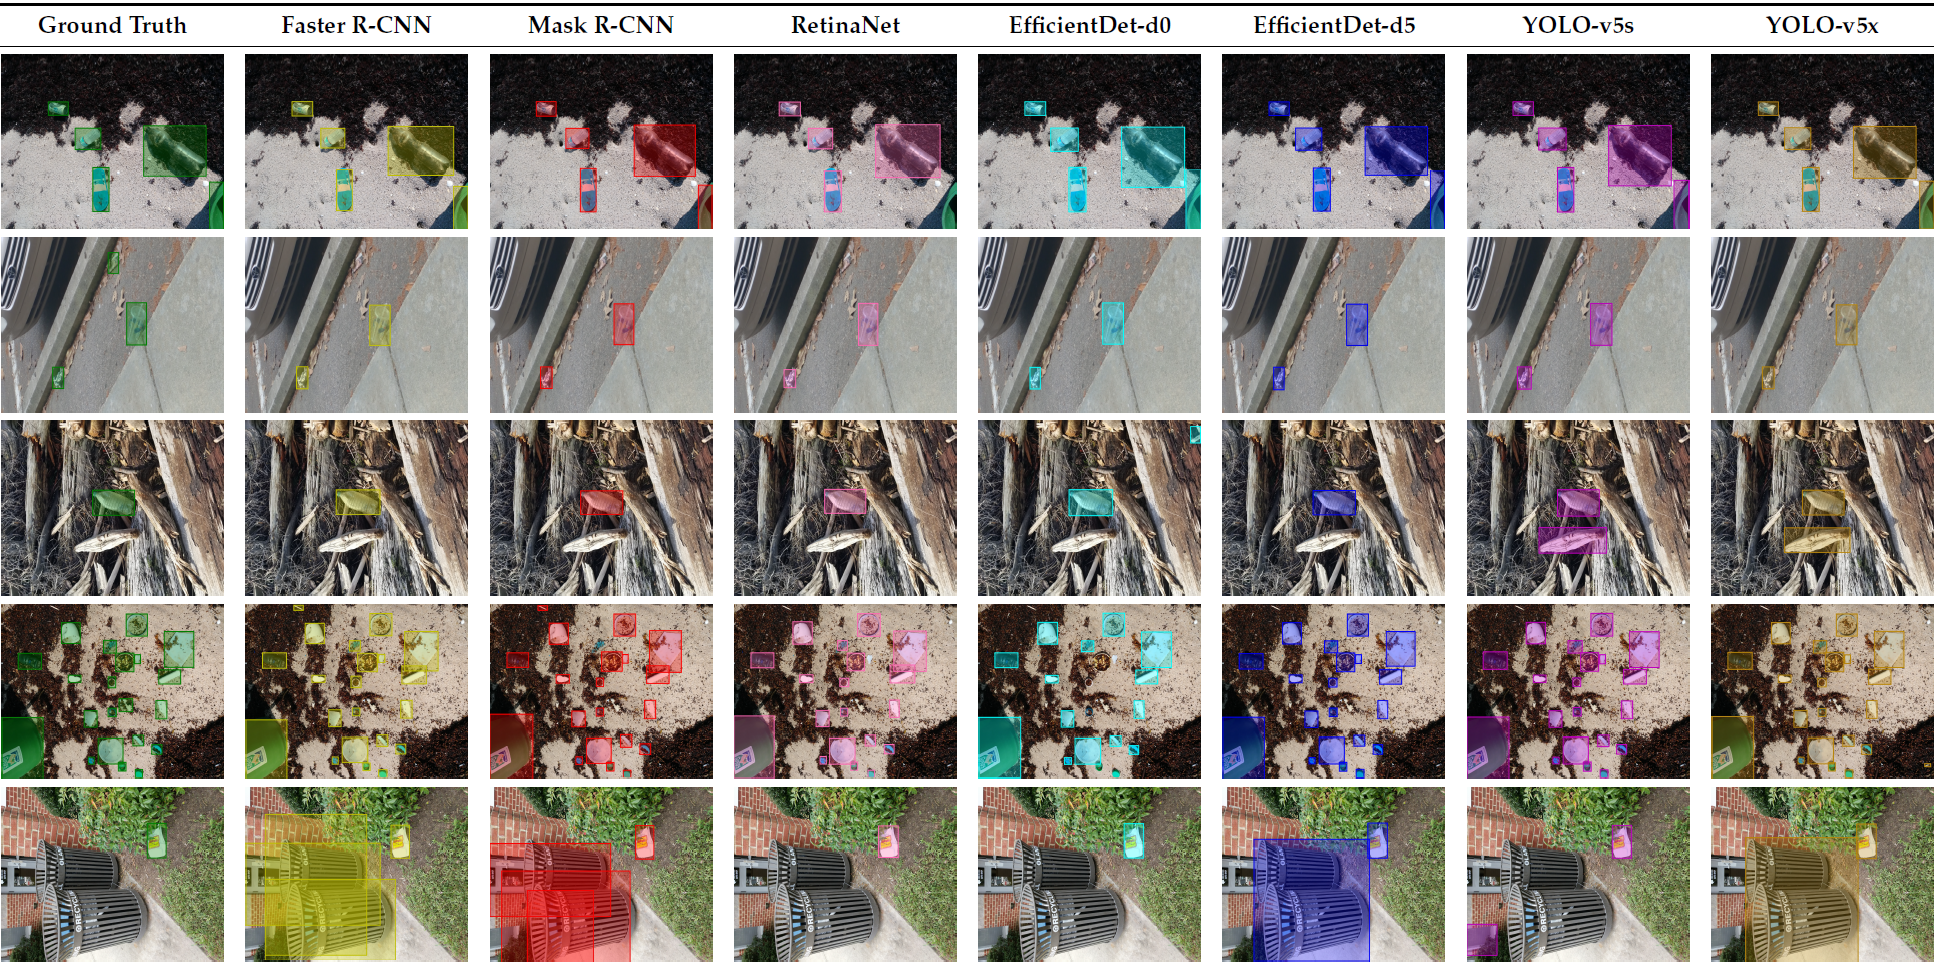
\includegraphics[width=1\linewidth]{plastopol.png}
    \caption{Visual detection results on the PlastOPol dataset. (Source: \cite{plastopol})}
    \label{fig:plastopol}
\end{figure}

To assess the performance of various deep learning models in detecting litter, the authors used both the proposed PlastOPol dataset and the publicly available \gls{taco} dataset. For the PlastOPol dataset, the data was split into 80\% for training and 20\% for testing. Evaluation metrics included \gls{ap}, \gls{map} at \gls{iou} threshold 0.5, F1 score, and recall. The models tested included EfficientDet, Faster \gls{rcnn}, Mask \gls{rcnn}, RetinaNet, and \gls{yolo}v5. As shown in Figure \ref{fig:plastopol}, the visual detection results on the PlastOPol dataset highlight the performance of these models in identifying litter objects across different environments.
The experiment results demonstrated that \gls{yolo}v5 was the best-performing model overall. The authors also observed that \gls{yolo}v5 and EfficientDet were the fastest models, even when deployed on mobile devices. However, they noted that all methods struggled with detecting small objects, such as cigarette butts. Notably, \gls{yolo}v5x outperformed Faster \gls{rcnn} and Mask \gls{rcnn} in terms of speed \cite{plastopol}.

\subsection{Real-Time UAV Trash Monitoring System}
\label{subsec:3_haida}

In 2022, Liao and Juang developed a marine litter detection system using \glspl{uav} \cite{haida}. Their goal was to reduce reliance on manual efforts and offer a more efficient method for identifying marine debris. The real-time \gls{uav} trash monitoring system consisted of nine components: \glspl{uav}, a message queuing system, a database, a video streaming server, a connector, a \gls{uav} control station, a web service, a \gls{uav} map, and a data analysis module, as illustrated in Figure \ref{fig:haida1}. The ground station incorporated key elements, such as the video streaming server, Kafka, the Kafka connector, MongoDB, and the web service. The system addressed two key challenges: object detection and geolocation, and as part of the system's development, the authors introduced the HAIDA dataset. This dataset, collected on the NTOU campus, was used to train the object detection model and contains two types of litter objects: \textit{garbage} and \textit{bottles}. The data was gathered using a \gls{uav} equipped with a Pixhawk controller and an NVIDIA Jetson Xavier NX. The UAV operated at altitudes ranging from 1 to 10 metres \gls{agl} \cite{haida}.

\begin{figure}[!htbp]
    \centering
    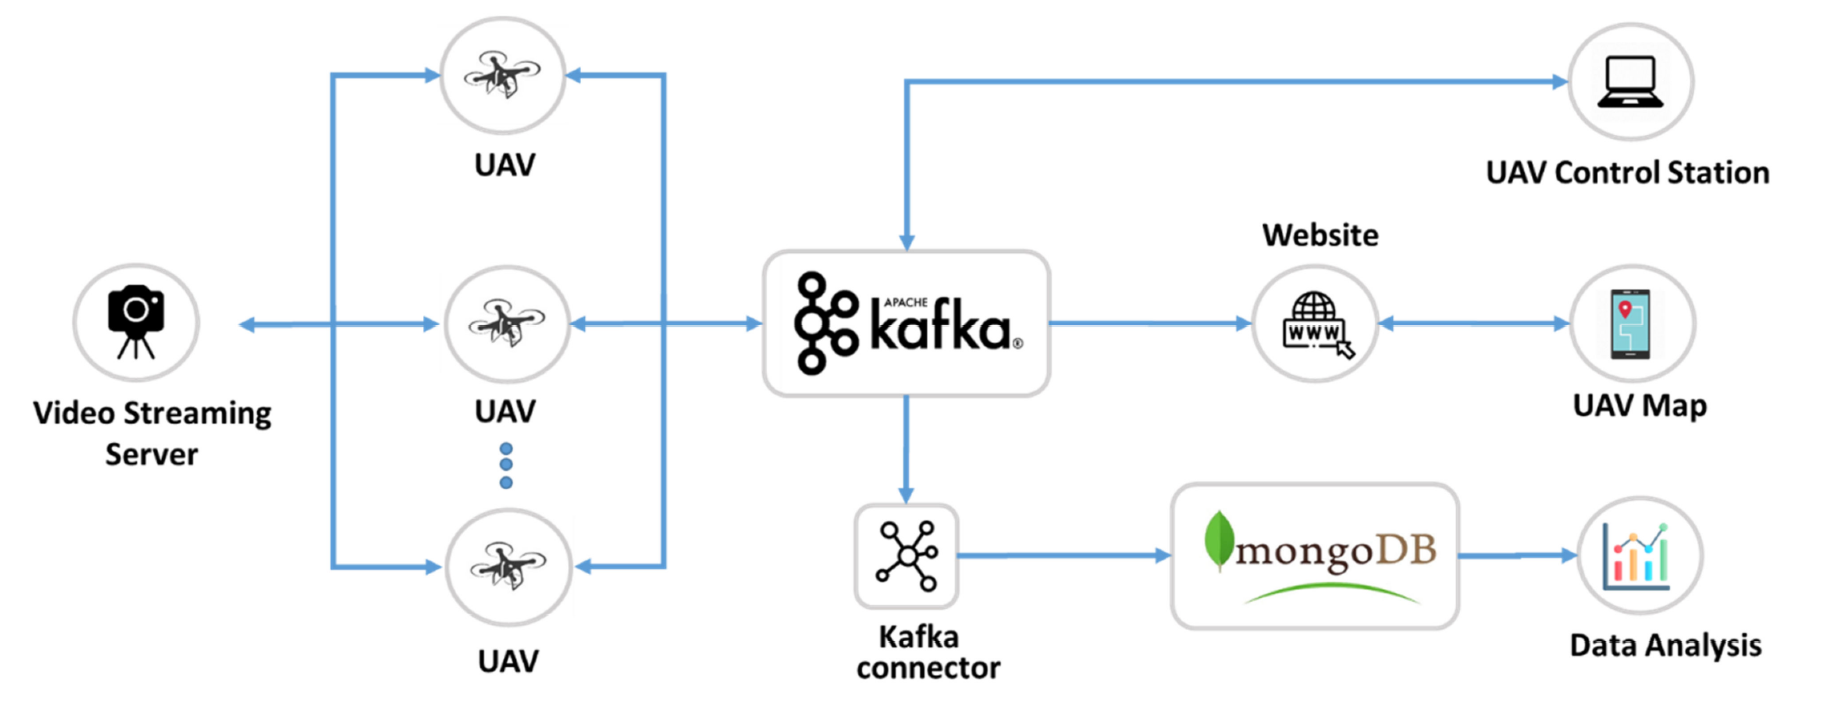
\includegraphics[width=0.9\linewidth]{haida1.png}
    \caption{The system architecture of the real-time \gls{uav} trash monitoring system. (Source: \cite{haida})}
    \label{fig:haida1}
\end{figure}

The HAIDA dataset comprises 1,319 annotated images, with 6,475 instances of litter, including 3,904 garbage objects and 2,571 bottle objects. Additionally, 456 images in the dataset contain no litter. The authors utilised the dataset to train a \gls{yolo} object detection model (version unspecified). The results showed that the model was able to identify trash objects with an \gls{ap} of over 70\% at a 0.5 \gls{iou} threshold. Notably, as shown in Figure \ref{fig:haida2}, the detection confidence for small objects was high, with confidence scores of 98.27\%, 64.65\%, and 91.86\% for different categories of litter.
The real-time \gls{uav} trash monitoring system operated by first collecting \gls{uav} footage as the drone flew across predetermined waypoints. The footage was then transmitted to a server via Kafka, where it was stored in an online database such as Oracle, MySQL, or MongoDB. Using this stored data, the server applied the trash detection model to identify litter both in the images and on a map. Control stations, both mobile and desktop, could make requests to the server to retrieve the map data, which displayed the locations of detected litter \cite{haida}.
To estimate litter geolocation, the authors followed an approach similar to that in \cite{uavvaste}, calculating pollution area based on \gls{uav} altitude, camera angles, and object size in the image. This enabled a reliable approximation of both the position and extent of detected waste \cite{haida}.

\begin{figure}[!htbp]
  \centering
  \begin{tabular}{cc}
    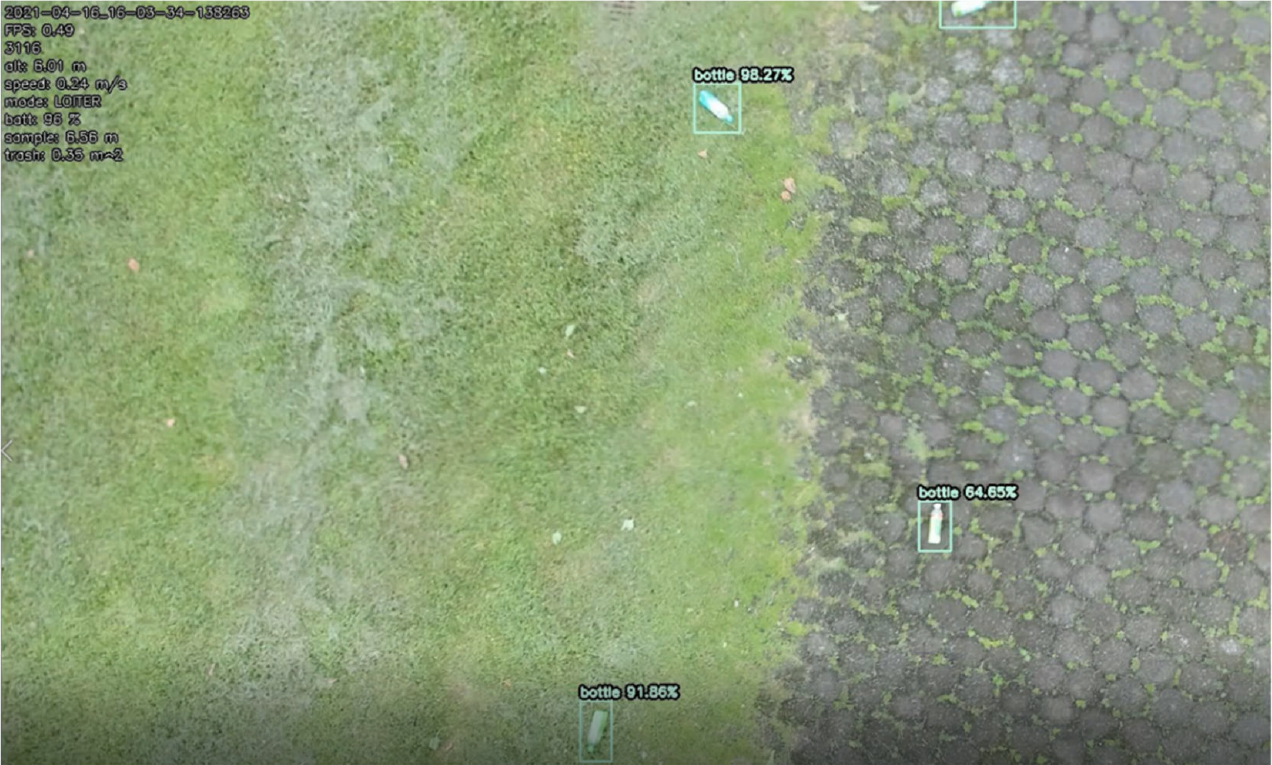
\includegraphics[width=0.48\textwidth, height=5cm]{haida2.png} &
    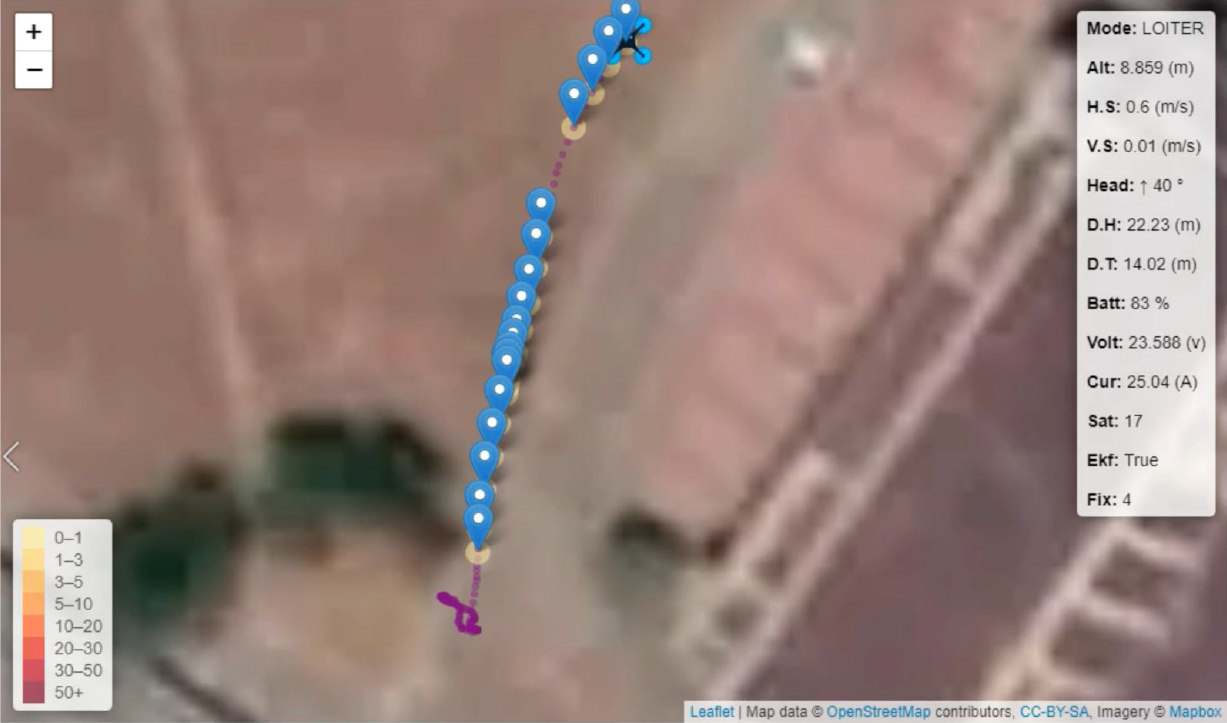
\includegraphics[width=0.48\textwidth, height=5cm]{haida3.png} \\
    \small (a) & \small (b) \\
  \end{tabular}\\
  \caption{\gls{uav} trash monitoring results on the NTOU campus. (a) Detection results from the UAV. (b) Detected litter plotted on a map, showing real-time monitoring and detection. (Source: \cite{haida})}
  \label{fig:haida2}
\end{figure}

% To tackle the problem of litter geolocation, the authors adapted a similar approach to the one described in \cite{uavvaste}, enabling the calculation of the detected trash pollution area based on several factors. These factors include the camera’s horizontal and vertical angle of view, the UAV’s altitude, the camera's field of view, the dimensions of the camera's image, the size of the detected trash in the image, and the detected trash's area in both the image and the real-world environment. By incorporating these variables, the system can accurately estimate the location and extent of trash pollution in the area \cite{haida}.

\subsection{Outdoor Trash Detection in Natural Environment}
\label{subsec:3_bangladeshi}

As populations in underdeveloped nations continue to grow, the challenges associated with trash production and disposal have become more urgent. Aware of the time-consuming and potentially hazardous nature of manual litter classification, Das et al. (2023) aimed to tackle this issue by developing automated methods for more efficient and safer waste management \cite{bangladeshi}. To achieve this, they focused on collecting data that accurately captured the complexities of litter in Bangladesh, creating an outdoor dataset, and incorporating OpenLitterMap to broaden its scope. This dataset comprises images from natural settings, not \gls{uav}-based data, and includes ten categories of litter: \textit{tissue paper}, \textit{plastic}, \textit{medical waste}, \textit{rope}, \textit{paper}, \textit{cigarette butts and boxes}, \textit{metal}, \textit{glass}, \textit{organic waste}, and \textit{textiles}. Initially consisting of 1,283 annotated images, the dataset was expanded to 4,418 by integrating data from OpenLitterMap, a global database containing litter and plastic images. The Bangladeshi dataset contains 6,178 instances of litter, which was extended to 8,077 while retaining the ten distinct classes \cite{bangladeshi}.

\begin{figure}[!htbp]
  \centering
  \begin{tabular}{c}
    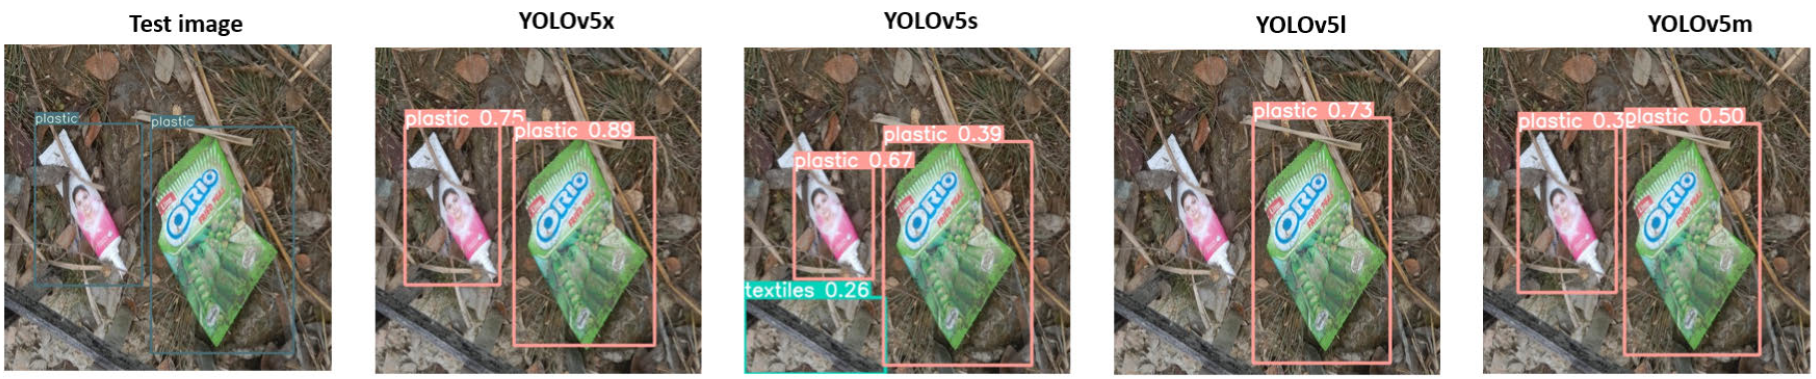
\includegraphics[width=1\textwidth]{bangladeshi1.png} \\
    \small (a)\\
    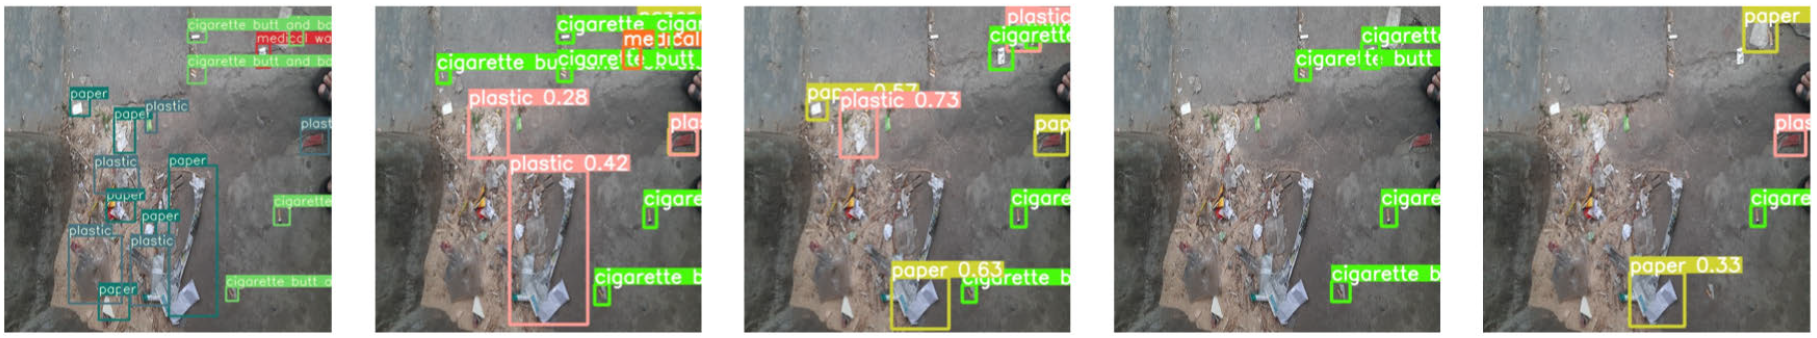
\includegraphics[width=1\textwidth]{bangladeshi2.png} \\
    \small (b) \\
  \end{tabular}\\
  \caption{Litter detection results using different versions of the \gls{yolo}v5 model on the Bangladeshi dataset. (a) 2 instances of litter; (b) 17 instances of litter. (Source: \cite{bangladeshi})}
  \label{fig:bangladeshi}
\end{figure}

The experimental setup used for this study involved a comparison with the \gls{taco} and PlastOPol datasets. The Bangladeshi dataset was divided as follows: 80\% for training, 10\% for validation, and 10\% for testing. The evaluation metrics included \gls{ap} and \gls{map} at \gls{iou} thresholds from 0.5 to 0.95, as well as F1 score and recall. Several models were tested, including different versions of \gls{yolo}v5, \gls{yolo}v6, \gls{yolo}v8, and Faster \gls{rcnn}. The authors also employed data augmentation techniques during training and optimised model performance by adjusting hyperparameters.
In their study, the authors reported that \gls{yolo}v5x was the best-performing model, as visually demonstrated in Figure \ref{fig:bangladeshi}, which shows a comparison of the detection bounding boxes on the images, demonstrating the improved \gls{map} for the expanded dataset. However, single-class detection experiments on the \gls{taco} and PlastOPol datasets yielded better results compared to the Bangladeshi dataset. Das et al. also highlighted that in future work, they plan to expand the dataset to include a broader range of categories, such as ocean waste, which is currently absent. Additionally, other object detection methods, such as \gls{ssd}, Mask \gls{rcnn}, and EfficientDet, could also be evaluated using their dataset \cite{bangladeshi}.

\subsection{Use of UAVs and Deep Learning for Beach Litter Monitoring}
\label{subsec:3_beach_litter}

In 2023, Pfeiffer et al. proposed a framework for an autonomous beach litter monitoring and retrieval system based on drone surveys and object detection using deep learning techniques \cite{beach_litter}. Their research combined drone footage collected from the islands of Malta and Gozo, Sicily (Italy), and the Red Sea coast with publicly available litter datasets, which were subsequently used to train an object detection model for identifying litter in the captured footage. Figure \ref{fig:beachlitter1} illustrates the overall framework of the proposed beach litter monitoring system. To address both object detection and geolocation challenges, the authors compiled a \gls{uav} dataset collected with a DJI Phantom 4 Pro 2.0 and a DJI Mavic 2 UAVs. The dataset covered altitudes ranging from 10 metres above ground level to 60 metres above sea level and included 67 types of litter, which were categorised into seven meta-classes: \textit{clothing \& fabric}, \textit{glass}, \textit{small objects}, \textit{metal litter}, \textit{paper \& cardboard}, \textit{plastic}, and \textit{other waste}.
Additionally, the collected Beach Litter Dataset contains 4,126 annotated images and 10,611 litter instances, including 1,154 images with no litter present. The dataset was divided as follows: 60\% for training, 20\% for validation, and 20\% for testing. The models were evaluated using metrics such as \gls{ap},\gls{map} (at 0.5–0.95), F1 score, and recall, with the \gls{yolo}v5 model being the primary model used for training \cite{beach_litter}. 

\begin{figure}[!htbp]
    \centering
    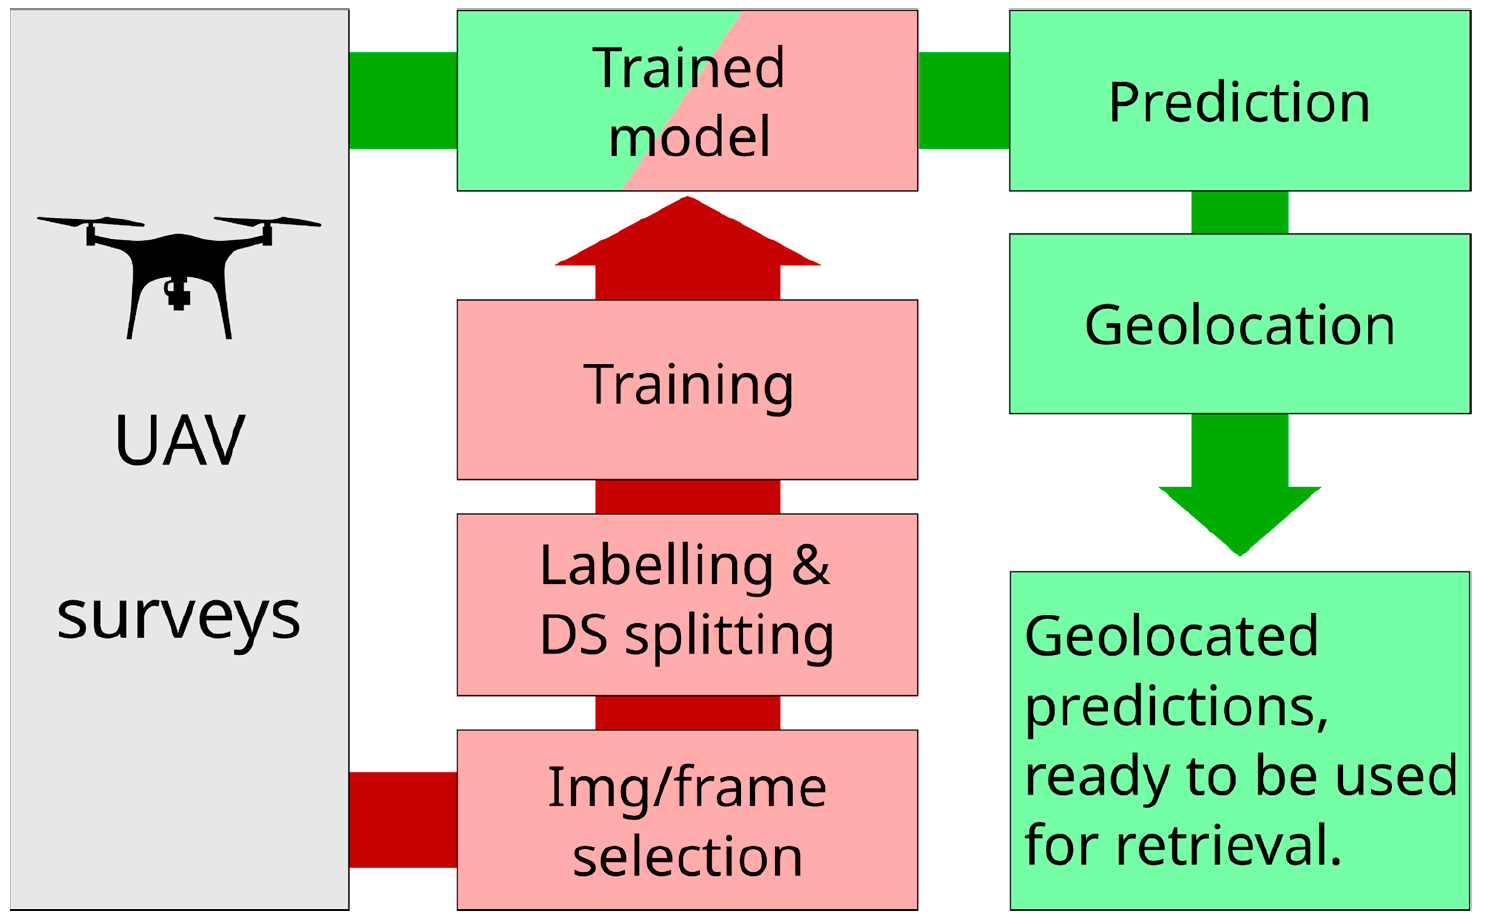
\includegraphics[width=0.7\linewidth]{beachlitter1.png}
    \caption{The system architecture of the real-time \gls{uav} beach litter monitoring and geolocation system, highlighting the two main pipelines: training (in red) and prediction (in green). (Source: \cite{beach_litter})}
    \label{fig:beachlitter1}
\end{figure}

% The authors also developed a geolocation algorithm to enhance the utility of the detected litter by integrating it with a robot for debris retrieval. For the algorithm to communicate the detection coordinates to the robot, the predictions made by the \gls{yolo}v5 model needed to be geolocated. This required that the original footage include \gls{gps} coordinates of the drone. The geolocation process involved several key steps: calculating the pixel size of the footage, determining the distance between meridians and parallels at the latitude of recording, measuring the horizontal and vertical distance from the prediction box's centre to the image centre, and transforming these distances into real-world coordinates. Figure \ref{fig:beachlitter2} shows the schematic for calculating litter geolocations, highlighting the parameters used to map the detected litter to real-world coordinates. To improve accuracy, the authors also calculated the distance between each litter object and the camera’s field of view, factoring in variables such as the \gls{uav}’s height and the angle of the camera’s lens. This enabled precise localisation of litter in both the image and the real-world environment, essential for guiding the robot to specific debris \cite{beach_litter}.

% \begin{figure}[!htbp]
%     \centering
%     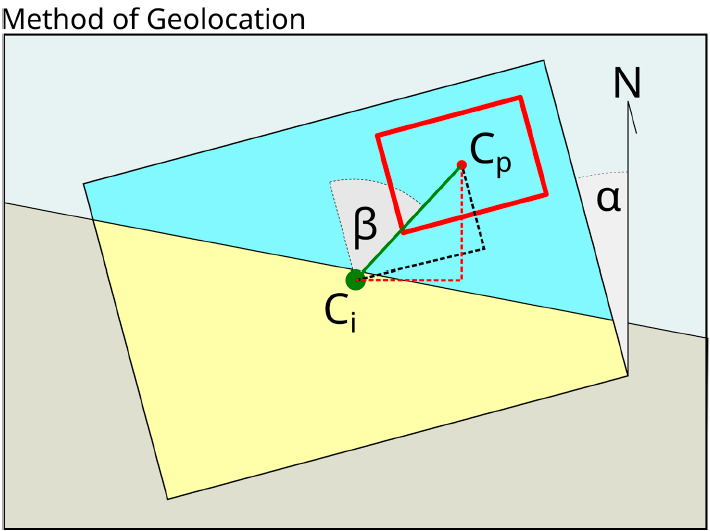
\includegraphics[width=0.7\linewidth]{beachlitter2.png}
%     \caption{Schematic representation of the calculation of litter geolocations, illustrating the parameters used to map the detected litter to real-world coordinates. (Source: \cite{beach_litter})}
%     \label{fig:beachlitter2}
% \end{figure}
The authors also created a geolocation algorithm to link detected litter with a debris-retrieving robot, requiring that detection coordinates be translated into real-world positions. This process used \gls{gps}-tagged footage and involved calculating pixel dimensions, spatial distances, and converting image offsets into geographic coordinates. Accuracy was further refined by incorporating \gls{uav} height and camera angle, ensuring reliable localisation for robotic retrieval \cite{beach_litter}.
The results of their experiments using the \gls{yolo}v5 model on the labelled dataset were as follows: precision of 0.695, recall of 0.288, \gls{map}@50 of 0.314, and \gls{map}@50-95 of 0.2. The model performed most reliably on the following ten classes: \textit{plastic bottle}, \textit{metal can}, \textit{plastic bottle} \textit{cap}, \textit{plastic container}, \textit{shoe}, \textit{cardboard}, \textit{pop tab}, \textit{rope \& string}, \textit{wood}, and \textit{glass bottle} \cite{beach_litter}.

\subsection{TrashNet: Real-Time Object Detection for Trash Classification}
\label{subsec:3_trashnet}

In 2024, Veeravadivel Santhanalakshmi, and Nguyen introduced TrashNet, an object detection model designed to classify images of waste in real time. The dataset employed to train the TrashNet network comprises six primary categories of litter: \textit{cardboard}, \textit{glass}, \textit{metal}, \textit{paper}, \textit{plastic}, and \textit{general waste}. This dataset, derived from an image classification dataset on Kaggle, does not utilise \gls{uav}-based data. Furthermore, the TrashNet dataset comprises 2,524 annotated images, each featuring a single object instance. The authors explain that the dataset was divided into three subsets for model development: 70\% for training, 20\% for testing, and 10\% for validation.
In this study, the \gls{yolo}v5 object detection model was used, and its performance was evaluated using metrics such as \gls{map}, precision, recall, and F1 score. 
The authors highlight that the primary aim of this study was to develop a real-time system to assist individuals in identifying the correct bin for various types of waste near rubbish disposal areas, as seen in Figure \ref{fig:trashnet}. Notably, the model successfully fulfilled this objective, achieving an accuracy of 90\% on both the validation and testing sets \cite{trashnet}.

\begin{figure}[!htbp]
    \centering
    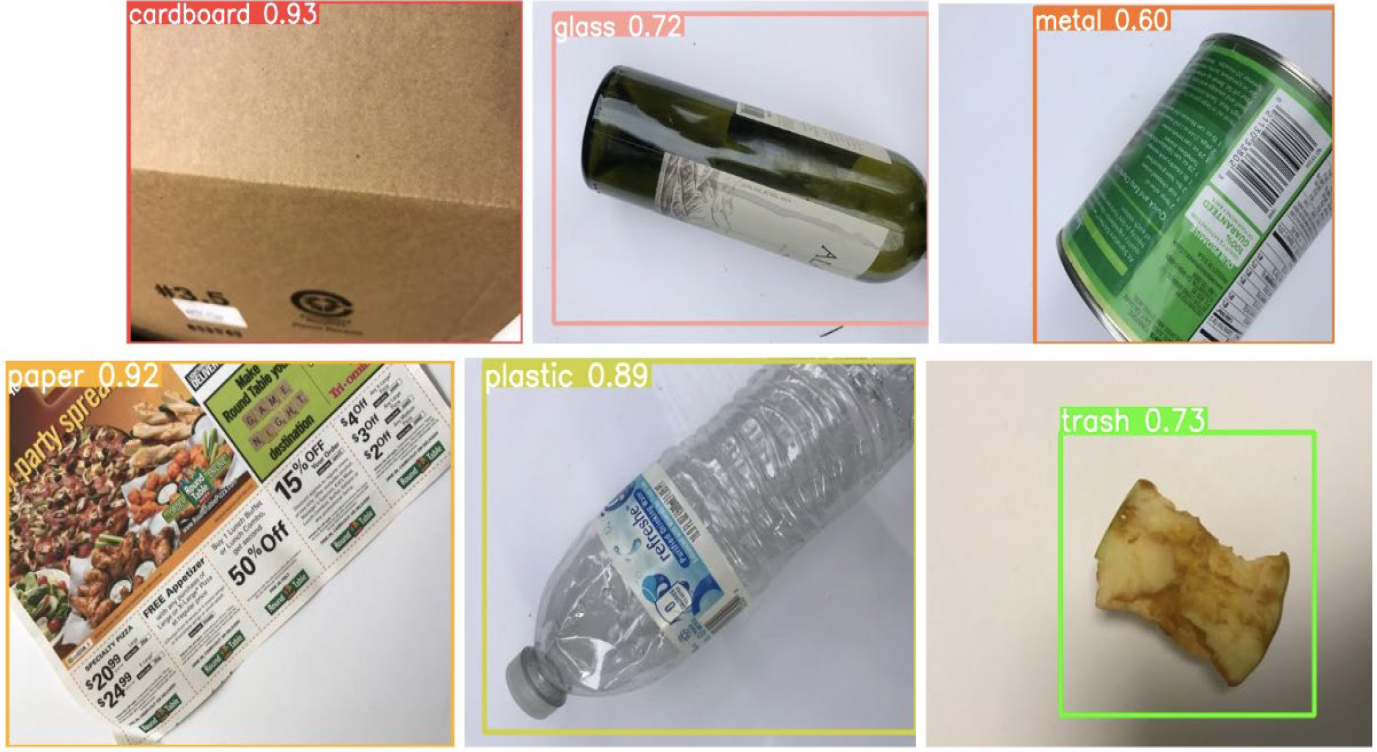
\includegraphics[width=0.8\linewidth]{trashnet.png}
    \caption{Litter detection results generated by the TrashNet detection model. (Source: \cite{trashnet})}
    \label{fig:trashnet}
\end{figure}

\subsection{SODA: Small Objects at Different Altitudes}
\label{subsec:3_sodadataset}

Modern \glspl{uav} are equipped with high-resolution cameras capable of capturing detailed pictures and videos of their surroundings. However, when the \gls{uav} is flying at higher altitudes, objects in the images may look very tiny, occupying only a few pixels. This poses substantial hurdles for spotting such objects. To tackle this issue, Pisani et al. (2024) introduced the \gls{soda} dataset, designed to aid research focused on small object detection in aerial imagery \cite{soda_dataset}. The dataset features six primary types of litter, derived from the \gls{taco} dataset: \textit{clear plastic bottles}, \textit{other plastic bottles}, \textit{glass bottles}, \textit{glass jars}, \textit{drinking cans}, and \textit{drinking cartons}. Figure \ref{fig:soda1} illustrates examples of litter categories used in the \gls{soda} dataset. Furthermore, the images were collected using a combination of DJI Mini 2 and DJI Air 2S UAVs at various altitudes, including 1m, 5m, 10m, 15m, 20m, 25m, and 30m \cite{soda_dataset, detect_litter}.

\begin{figure}[!htbp]
    \centering
    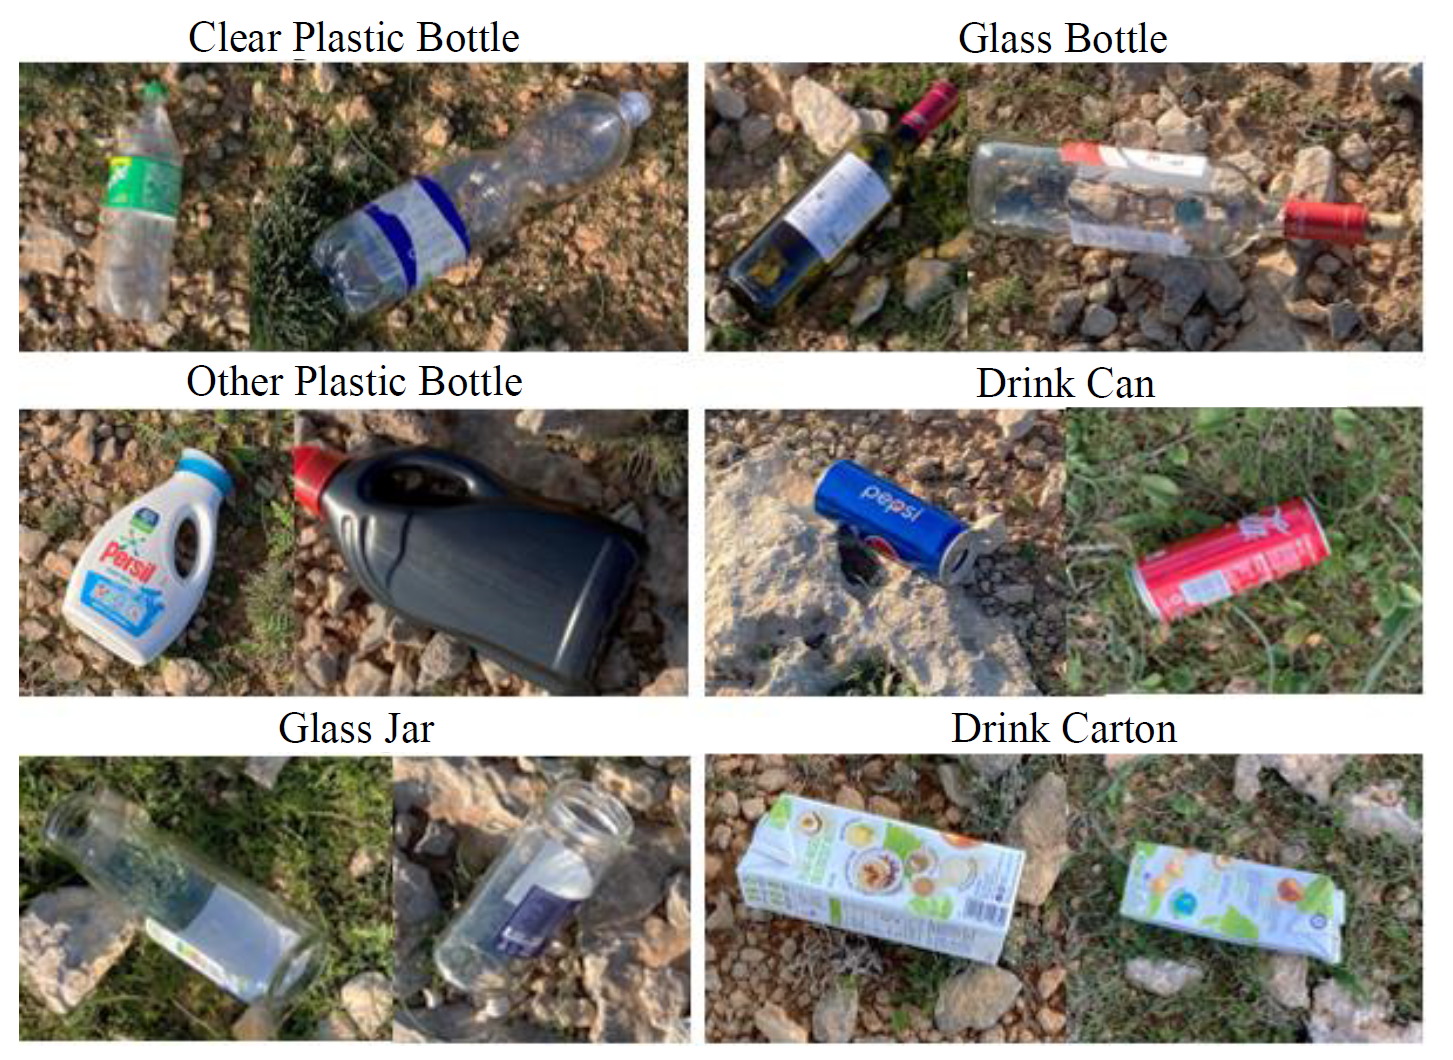
\includegraphics[width=0.8\columnwidth]{soda_images.png}
    \caption{The six object categories featured in the SODA dataset. (Source: \cite{soda_dataset})}
    \label{fig:soda1}
\end{figure}

The \gls{soda} dataset consists of 829 annotated images, with 452 (54.52\%) taken at 1 metre and 377 (45.48\%) captured from altitudes of 5 metres or more. 
The \gls{soda} dataset supports multi-class classification, with each object annotated with a distinct label using polygons rather than bounding boxes. The authors explain that polygons offer a more accurate fit around the object, whereas bounding boxes often capture additional background. Additionally, they clarify that polygons provide precise alignment during augmentations, such as rotation. Techniques for annotating with polygons and applying these augmentations are outlined in \cite{mask_to_annotation}. However, although the \gls{soda} dataset is annotated using polygons, the authors focus on the challenge of object detection rather than instance segmentation.
To address the challenge of detecting small objects across multiple categories of litter, the authors employed three different training strategies. The first approach involved segregating the training dataset according to altitude. In the second approach, the dataset was merged while maintaining multi-class labels. The third approach also merged the dataset, consolidating all categories into a single \textit{litter} class. 
Notably, a key feature of this study was the application of a \textit{tiling methodology} to improve the detection of small objects. This technique divides an image into a grid and splits it into smaller, equally sized sections, which were used in both the training and inference stages. The authors note that the grid size can significantly influence detection performance, with smaller grids, such as $2 \times 2$ (refer to Figure \ref{fig:soda2}), used at lower altitudes and larger grids, like $5 \times 5$, applied at higher altitudes. For the \gls{soda} dataset, a $5 \times 5$ grid was used across all altitudes and images \cite{detect_litter, soda_dataset, daniel_thesis}.

\begin{figure}[!htbp]
    \centering
    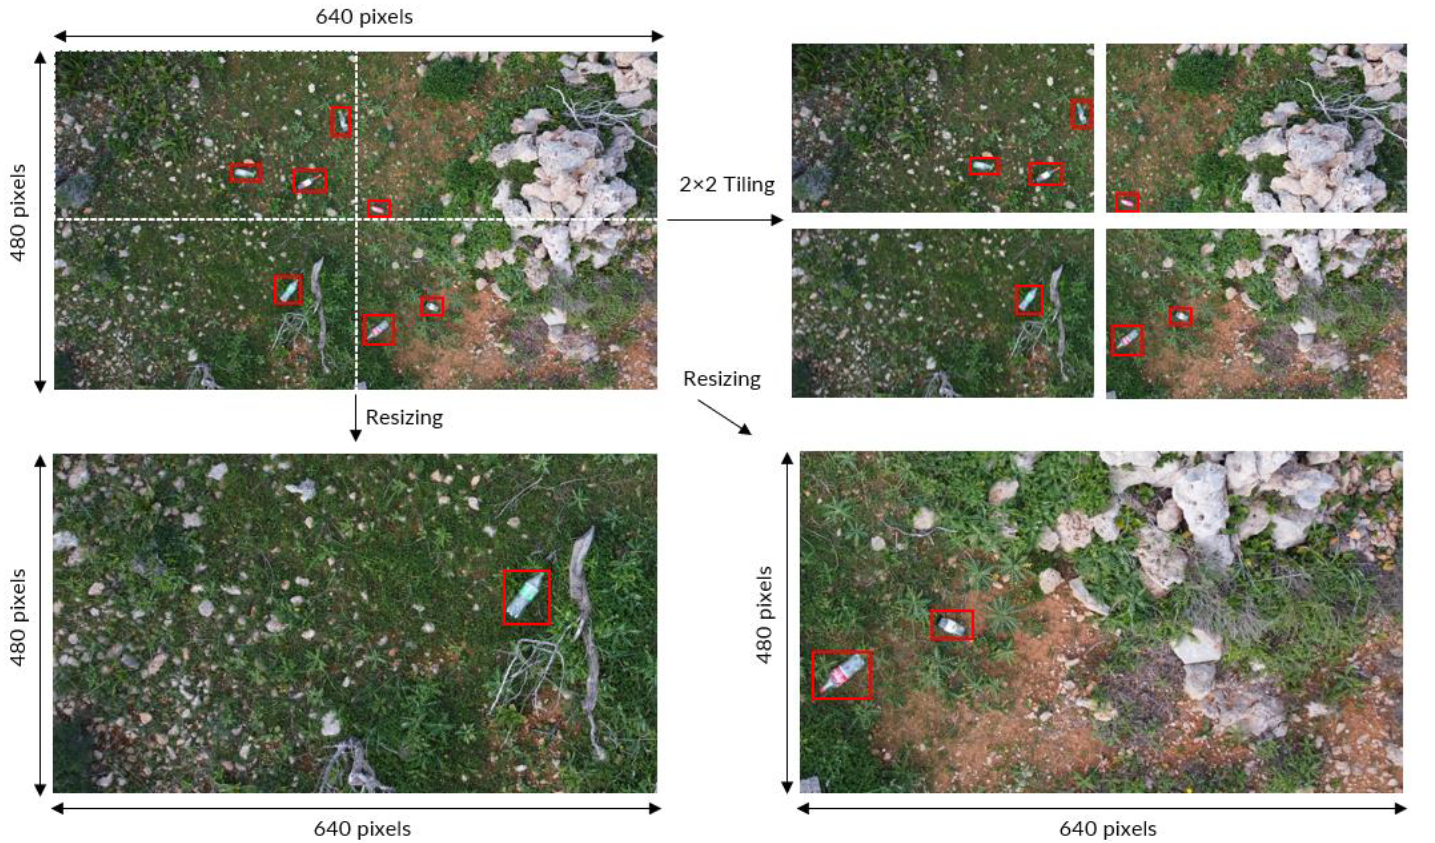
\includegraphics[width=1\columnwidth]{soda2.png}
    \caption{Application of a $2 \times 2$ tiling grid to aerial imagery captured at an altitude of 5 metres. (Source: \cite{detect_litter})}
    \label{fig:soda2}
\end{figure}

Three object detection models were trained for this study: \gls{yolo}v5 and \gls{yolo}v8 (both one-stage detectors) and Faster \gls{rcnn} (a two-stage detector). Models trained using the second and third approaches were evaluated on the \gls{bdw} dataset. The results indicated that the third approach, which merged all classes into a single litter category, outperformed the second approach. Additionally, the evaluation revealed that the \gls{soda} dataset was lacking a sufficient number of images of clear plastic bottles. 
In terms of \gls{map}, the results for the different models were as follows: Faster \gls{rcnn} achieved a \gls{map} of 0.921, \gls{yolo}v5 had a \gls{map} of 0.854, and \gls{yolo}v8 performed with a \gls{map} of 0.728 \cite{soda_dataset, detect_litter}. 
Conclusively, this study contributes to the use of \glspl{uav} for capturing aerial imagery and applying computer vision techniques to detect and classify objects within these images. The authors emphasise its significance as a crucial phase and a stepping stone towards the automation of litter collection for cleanup efforts \cite{detect_litter, soda_dataset, daniel_thesis}.

\subsection{Discussion}
\label{subsec:3_discussion}

The reviewed datasets and approaches highlight the growing potential, and popularity of \gls{uav}-based \gls{ai} systems for litter detection and management. While certain datasets were originally developed for recycling classification in indoor or controlled settings, others target outdoor environments, which present significantly greater challenges. Datasets that rely on \glspl{uav} are particularly affected by the difficulty of identifying small objects from aerial perspectives.
The variation across datasets reveals a wide range of technical and contextual difficulties associated with litter detection, as shown in Table \ref{tab:lit_review}. For example, datasets such as TrashNet \cite{trashnet}, MJU-Waste \cite{mju_waste}, and ZeroWaste \cite{zerowaste} were created under artificial conditions. In contrast, datasets like PlastoPol \cite{plastopol}, TACO \cite{taco2020}, and several \gls{uav}-oriented collections \cite{haida,soda_dataset,uavvaste,bdwdataset,beach_litter,superdock,umgeosurvey} contain real-world data collected in natural and urban environments.

Honing in on \gls{uav}-based litter deteciton, a recurring limitation evident in \gls{uav} datasets is the restricted number of annotated categories. In many cases, only one category is included. To this end, when multiple categories are included in a dataset, a common practice observed was to conduct an experiment by merging all classes into a single general litter category. Another challenge lies in the height at which data are collected. Most \gls{uav}-based datasets capture images at around 10 metres \gls{agl} or less. Exceptions such as \gls{bdw} \cite{bdwdataset} and \gls{soda} \cite{soda_dataset} extend this altitude to 30 metres, while the Beach Litter Dataset \cite{beach_litter} reaches up to 60 metres. Notwithstanding this, from among the \gls{uav} litter datasets only the \gls{soda} dataset \cite{soda_dataset} provides altitude-specific subsets of data.
Notably, the diversity of litter datasets and public accessibility is a key factor in supporting further development of \gls{ai}-based litter detection systems. Although several of the reviewed datasets have been featured in international peer-reviewed conferences and journals, only a limited number are available to the public. As illustrated in Table \ref{tab:lit_review}, the publicly accessible datasets include \gls{bdw} \cite{bdwdataset}, \gls{taco} \cite{taco2020}, MJU-Waste \cite{mju_waste}, UAVVaste \cite{uavvaste}, ZeroWaste \cite{zerowaste}, PlastoPol \cite{plastopol}, HAIDA \cite{haida}, TrashNet \cite{trashnet}, and \gls{soda} \cite{soda_dataset}, with just four of these specifically developed for \gls{uav} applications.

In terms of detection methods, \textit{data augmentation} is frequently employed to improve model performance. This is a common practice across both \gls{uav} and ground-based approaches. Techniques such as image \textit{tiling} or \textit{slicing} are especially important to facilititate \gls{uav}-based litter detection. High-resolution drone footage, often recorded in 4K, provides greater visual detail, which helps in identifying smaller objects. However, standard object detection models typically require downscaled inputs, ranging between $640$ and $1280$ pixels. This reduction can enable small litter objects even harder to detect. Splitting the original image into smaller tiles helps to preserve object size and minimise the loss of pixel detail. Nevertheless, proper experimentation of this method must be ensured, as adopting this process increases the computational load.

% Table \ref{tab:lit_review} presents a systematically organised comparison of the datasets and approaches, highlighting that the three primary challenges addressed were object detection, instance segmentation, and object geolocation, spanning both \gls{uav}-based and non-\gls{uav} datasets. It is also evident that for \gls{uav}-based approaches, altitudes ranging from 10 metres to 30 metres were the most commonly used. Additionally, in terms of the number of categories or litter types represented across datasets, both \gls{uav} and non-\gls{uav} approaches predominantly focus on creating single-class labelled datasets, with a few exceptions, such as recent approaches employing 6 to 10 classes, excluding the Beach Litter \cite{beach_litter} and \gls{taco} \cite{taco2020} datasets. Additionally, despite non-UAV datasets often containing a relatively large number of images, most \gls{uav}-based datasets consist of a smaller number of images, with notable exceptions being the \gls{bdw} \cite{bdwdataset} and Beach Litter \cite{beach_litter} datasets.

\begin{table*}[htbp]
\centering
\scriptsize
\begin{adjustbox}{max width=\textwidth, center}
\renewcommand{\arraystretch}{2.0}%1.5
\begin{tabular}{|l|c|c|c|c|c|c|c|}%|l|l|
\hline
\textbf{Name} & \textbf{Year} & \textbf{No of. Images} & \textbf{UAV}& \textbf{AGL Altitudes} & \textbf{Dataset Details}& \textbf{No of. Categories}  & \textbf{Available}\\ 
\hline \hline
\textbf{BDW Dataset \cite{bdwdataset}} & 2018 & 25,407 & Yes & 10m--30m & Detection & 1 (Litter)  &Yes\\ \hline
\textbf{UM Geo. Survey \cite{umgeosurvey}} & 2018 & 472 & Yes & 30m & Data Collection & 5 (Litter)  &No\\\hline
\textbf{SuperDock \cite{superdock}} & 2019 & 100 & Yes & 5m--10m & Detection & 1 (Litter)  &No\\\hline
\textbf{Styrofoam Monitoring \cite{styrofoam}} & 2019 & N/S\footnotemark[1] & Yes & 15m & Detection, Segmentation & 1 (Litter)  &No\\\hline
\textbf{Small Litter Detection \cite{small_litter_detection}} & 2019 & 744 & Yes & 5m--10m & Detection & 1 (Litter)  &No\\\hline
\textbf{TACO Dataset \cite{taco2020}} & 2020 & 1,500 & No & N/A\footnotemark[2] & Detection, Segmentation & 60 (Litter) [28 Super]  &Yes\\\hline
\textbf{MJU-Waste Dataset \cite{mju_waste}} & 2020 & 2,475 & No & N/A\footnotemark[2] & Segmentation & 1 (Litter)  &Yes\\\hline
\textbf{UAVVaste Dataset \cite{uavvaste}} & 2021 & 772 & Yes & low-altitude & Detection, Geolocation & 1 (Litter)  &Yes\\\hline
\textbf{ZeroWaste Dataset \cite{zerowaste}} & 2022 & 10,715 & No & N/A\footnotemark[2] & Detection, Segmentation & 4 (Litter)  &Yes\\\hline
\textbf{PlasOPol Dataset \cite{plastopol}} & 2022 & 2,418 & No & N/A\footnotemark[2] & Detection & 1 (Litter)  &Yes\\\hline
\textbf{HAIDA Dataset \cite{haida}} & 2022 & 1,319 & Yes & 1m--10m & Detection, Geolocation & 2 (Litter)  &Yes\\\hline
\textbf{Bangladeshi Dataset \cite{bangladeshi}} & 2023 & 4,418 & No & N/A\footnotemark[2] & Detection & 10 (Litter)  &No\\\hline
\textbf{Beach Litter Dataset \cite{beach_litter}} & 2023 & 4,126 & Yes & 10m--60m & Detection, Geolocation & 67 (Litter) [7 Super]  &No\\\hline
\textbf{TrashNet \cite{trashnet}} & 2024 & 2,524 & No & N/A\footnotemark[2] & Detection & 6 (Litter)  &Yes\\\hline
\textbf{SODA Dataset \cite{soda_dataset}} & 2024 & 829 & Yes & 1m, 5m--30m & Detection, Segmentation & 6 (Litter) [4 Super]  &Yes\\\hline
\end{tabular}
\renewcommand{\arraystretch}{1}
\end{adjustbox}
\caption{Comparison of datasets and approaches, systematically organised, with litter-related images captured from both \gls{uav} and non-\gls{uav} data.}
\label{tab:lit_review}
\end{table*}

\footnotetext[1]{N/S: The amount of images was not specified.}
\footnotetext[2]{N/A: Not applicable for non-\gls{uav}-based litter detection datasets.}

In addressing the problem of litter detection, most studies rely on deep learning models. The most commonly used architectures include variants of \gls{yolo} \cite{yolo, yolov5, yolov8}, along with Faster \gls{rcnn} \cite{fasterrcnn}, RetinaNet \cite{retinanet}, \gls{ssd} \cite{ssd}, and EfficientDet \cite{efficientdet}. A typical approach involves using these general object detection models as out-of-the-box solutions for the task \cite{soda_dataset, detect_litter, plastopol, beach_litter}. Other studies, such as those by \cite{small_litter_detection, styrofoam}, have explored modifications to the architecture and incorporated techniques such as background removal and \gls{cam} to improve results.
Additionally, some methods \cite{taco2020, mju_waste, zerowaste} approach the problem not just as an object detection problem but also as one of litter instance segmentation. In this regard, models like DeepLabv3 \cite{deeplabv3} and Mask \gls{rcnn} \cite{maskrcnn} have gained prominence. Interestingly, other \gls{uav}-based approaches \cite{beach_litter,haida,uavvaste} aim to address litter geolocation or georeferencing. These methods develop algorithms based on drone properties and mathematical formulas, allowing integration with the detection outputs to determine the precise locations of the detected litter.


\section{Review of Learning Using Privileged Information in Computer Vision}
\label{subsec:2_lupi}
% Glorja lil Missier u lil-iben u lil-Ispirtu Santu, Kif kien mill-bidu issa ghal dejjem ta' dejjem. Amen. Salve Regina

% At the time of writing this dissertation, no prior research has applied the \gls{lupi} paradigm within the problem of object detection. The most closely related work lies within the broader field of computer vision, where the application of \gls{lupi} remains relatively sparse. In this domain, many tasks exhibit an asymmetry in the availability of information between the training and testing phases \cite{learning2rank}, rendering \gls{lupi} particularly relevant.

At the time of writing this dissertation, the application of the \gls{lupi} paradigm within object detection remains underexplored. One early attempt is the work of Feyereisl et al. (2014) \cite{lupi_od_extra1}, who employed segmentation masks and \gls{surf} features as privileged information for object localisation. Their approach enabled a Structural SVM+ algorithm to incorporate privileged information on the Caltech-UCSD Birds 2011 dataset \cite{birds_dataset}. However, this study is relatively old, addressed only the problem of general localisation, and did not involve modifications to deep learning–based object detection models. The reported improvements from privileged information were also marginal. A later study by Sun et al. (2018) \cite{lupi_od_extra2} also used the Caltech-UCSD Birds dataset to examine localisation with privileged information. In their work, segmentation masks were applied to a subset of images where the birds appeared relatively large and well-defined. The method, based on the \gls{jkse} algorithm \cite{jkse} and evaluated on this subset, achieved only limited improvements in localisation accuracy as measured by the \gls{iou} metric. These works highlight that research on \gls{lupi} in detection and localisation remains at an early stage. More broadly, in computer vision, applications of \gls{lupi} are still sparse, even though many tasks involve an asymmetry between the information available during training and that at test time \cite{learning2rank}, a setting where \gls{lupi} is particularly relevant.

Sharmanska et al. \cite{learning2rank, learning2rank2} explore four distinct forms of privileged information for image classification: semantic attributes, bounding boxes, textual descriptions, and annotator rationale. Their experiments apply these types of privileged information within a rank transfer framework compatible with SVM solvers, focusing on the SVM+ algorithm. Their findings indicate a measurable improvement in classification performance when \gls{lupi} is integrated into the learning process \cite{learning2rank, learning2rank2}.
In a related contribution, Wang et al. \cite{lupi_classification} also address multi-label image classification by incorporating privileged information during training. Their approach employs similarity constraints derived from privileged inputs, along with ranking constraints informed by multiple labels, to develop a more effective classifier. High-resolution images and associated image tags serve as the privileged data, available solely during training. The method is evaluated across several benchmark datasets, and the results suggest that the inclusion of privileged information, alongside an awareness of label dependencies, contributes meaningfully to improved model performance \cite{lupi_classification}.

Although not directly related to \gls{lupi}, a substantial body of work aligns conceptually through the use of knowledge distillation techniques within computer vision \cite{distillation1, distillation2}. Knowledge distillation is a prominent method in machine learning, facilitating the transfer of information from a high-capacity model to a smaller, more efficient counterpart \cite{hinton_distillation}. This process enables the distilled model to retain essential predictive capabilities while reducing computational overhead.

In the context of vision-based tasks, various distillation methods have been explored, including those based on output responses, internal feature representations, and inter-feature relationships \cite{distillation1}. These techniques are applicable across a range of visual domains, including image classification, object detection, and multimodal frameworks. Specific to object detection, two widely adopted strategies are feature imitation and logit matching, which aim to replicate intermediate activations and output distributions respectively \cite{distillation2}.
A noteworthy development is the concept of localisation distillation, as proposed in \cite{distillation2}, which refines the transfer process by concentrating on spatial regions deemed informative for both classification and localisation. This targeted distillation allows the student model to better capture salient visual patterns by selectively attending to regions that contribute meaningfully to detection accuracy.

%  Evaluation Metrics
\section{Metrics}
\label{sec:4_metrics}
% Glorja lil Missier, lil-Iben, u lil-Ispirtu s-Santu kif kien mill-bidu issa u dejjem ghal-dejjem. Amen.

To objectively assess the performance of object detection systems, it is necessary to rely on standardised evaluation protocols. These metrics enable a consistent comparison between different models and methodologies, independent of the datasets or specific applications involved. In the context of object detection, evaluation typically involves comparing predicted bounding boxes and class labels against annotated ground truth data using metrics derived from the \gls{iou} criterion. This section outlines the most widely used performance metrics in vision-based detection tasks.

Performance is typically measured by comparing predicted bounding boxes and class labels against annotated ground truth using the \gls{iou} metric, which quantifies the overlap between predictions and actual annotations. The \gls{iou} threshold defines the minimum required overlap for a detection to be accepted as a true positive. Lower thresholds (e.g., 0.5) allow for more leniency, while higher thresholds (e.g., 0.75) enforce stricter accuracy requirements \cite{coco}. This threshold informs the calculation of standard indicators: \gls{tp}, which represent correctly detected objects; \gls{fp}, indicating incorrect or insufficient detections; and \gls{fn}, which refer to missed objects that appear in the ground truth. \gls{tn} are generally excluded from these evaluations, as they pertain to correct predictions of object absence.

% Having outlined the importance of datasets and identified those relevant to this study, it is essential to evaluate the quantitative performance of object detection techniques to gauge their effectiveness in addressing the detection problem, in line with objectives \textbf{O2} through \textbf{O4}. The evaluation of these systems primarily involves comparing model predictions (bounding boxes and labels) with ground truth annotations using the Intersection over Union (\gls{iou}) metric, which measures the overlap between predicted and actual bounding boxes. The \gls{iou} threshold determines the minimum overlap needed for a prediction to be considered a true positive. Lower thresholds (e.g., 0.5) allow for more flexible matching, whereas higher thresholds (e.g., 0.75) set stricter criteria \cite{coco}. This metric also facilitates the computation of important evaluation indicators: \gls{tp}, which are correctly identified objects with an \gls{iou} above the threshold; \gls{fp}, which are objects incorrectly identified or those with insufficient overlap; and \gls{fn}, which are objects missed by the model that are present in the ground truth. \gls{tn} are generally not included in object detection evaluations, as they correspond to the correct identification of the absence of an object.

\gls{iou}, or Jaccard’s Index, serves as a metric for evaluating the overlap between the predicted bounding box and the ground truth, offering a quantitative measure of the precision in object localisation. As demonstrated in Equation \ref{eqn:iou}, $b$ denotes the predicted bounding box, while $g$ refers to the ground truth. A higher \gls{iou} value, with a maximum of 1, signifies greater accuracy in the predictions, indicating a smaller deviation between the predicted bounding box and the ground truth.
\begin{equation}
\label{eqn:iou}
\text{IoU}(b, g) = \frac{{\text{area}(b \cap g)}}{{\text{area}(b \cup g)}}.
\end{equation}
Precision, as outlined in Equation \ref{eqn:precision}, measures the proportion of relevant items retrieved by the model. It is determined by the ratio of \gls{tp}, which are objects correctly identified as relevant, to the sum of \gls{tp} and \gls{fp}, which denotes the total number of objects that were mistakenly identified as relevant.
\begin{equation}
\text{Precision} = \frac{\text{TP}}{\text{TP} + \text{FP}} = \frac{\text{IoU}(b, g) > \text{threshold}}{\text{IoU}(b, g) > \text{threshold} + \text{FP}}.
\label{eqn:precision}
\end{equation}
\noindent
Recall, as presented in Equation \ref{eqn:recall}, evaluates the model's ability to identify all relevant items. Recall is calculated as the ratio of \gls{tp} to the sum of \gls{tp} and \gls{fn}, with \gls{fn} representing relevant objects that the model failed to detect.
\begin{equation}
\text{Recall} = \frac{\text{TP}}{\text{TP} + \text{FN}} = \frac{\text{IoU}(b, g) > \text{threshold}}{\text{IoU}(b, g) > \text{threshold} + \text{FN}}.
\label{eqn:recall}
\end{equation}
\noindent
The F1 Score, represented in Equation \ref{eqn:f1}, is the harmonic mean of precision and recall, offering a balanced evaluation of both. It is computed by taking the product of precision and recall, doubling it, and dividing by the sum of precision and recall, thereby reflecting the model's overall ability to identify relevant objects.
\begin{equation}
\text{F1 Score} = 2 \times \frac{\text{Precision} \times \text{Recall}}{\text{Precision} + \text{Recall}}.
\label{eqn:f1}
\end{equation}
\noindent
Average Precision (\gls{ap}), as outlined in Equation \ref{eqn:average_precision}, evaluates the overall precision at various recall levels, \( R_k \), where \( k \) represents a recall threshold between 0 and 1. \gls{ap} reflects the balance between \gls{fp} and \gls{fn}, providing a more nuanced evaluation of model performance. It can also be interpreted as the area under the precision-recall curve (AUC), with higher values signifying better model performance.
\begin{equation}
\text{Average Precision (AP)} = \sum_{k=0}^{n} (R_k - R_{k-1}) \cdot P_k.
\label{eqn:average_precision}
\end{equation}
\noindent
The Mean Average Precision (\gls{map}), as represented in Equation \ref{eqn:map}, computes the average precision across all \( N \) classes by summing the individual average precision values \( (\text{AP}_i) \) and dividing by the total number of classes. \gls{map} values range from 0 to 1, with higher values indicating better model performance.
\begin{equation}
\text{Mean Average Precision (mAP)} = \frac{1}{N} \sum_{i=1}^{N} \text{AP}_i.
\label{eqn:map}
\end{equation}
\noindent
The \gls{mar}, as defined in Equation~\ref{eqn:mar_coco}, measures the model's average recall across all \( N \) classes. For each class, recall is computed at several \gls{iou} thresholds, typically ranging from 0.50 to 0.95 in steps of 0.05. These per-class recall values are first averaged across \gls{iou} levels, then across all categories. This results in a single \gls{mar} score that reflects the model's ability to detect objects across varying overlap conditions. Additionally, \gls{mar} can be reported at different detection counts, such as \gls{mar}@1, \gls{mar}@10, and \gls{mar}@100. These settings restrict the evaluation to the top 1, 10, or 100 predicted boxes per image, respectively \cite{coco}.
\begin{equation}
\text{Mean Average Recall (mAR)} = \frac{1}{N} \sum_{i=1}^{N} \text{AR}_i(\text{IoU}).
\label{eqn:mar_coco}
\end{equation}
\noindent
The confusion matrix, shown in Equation~\ref{eq:confusion_matrix}, is a metric that summarises a classification network’s performance by reporting \gls{tp}, \gls{fp}, \gls{fn}, and \gls{tn} for each class. In the context of object detection, a background class (denoted as \( BG \)) is added to account for regions without objects. The matrix includes all object categories the model is trained to detect, collectively represented as the set \( C \). A strong diagonal in the matrix suggests high accuracy, indicating that predicted labels closely match the actual ones.
% \begin{equation}
% \text{Confusion Matrix}_c =
% \begin{array}{c|cc}
% & \text{Predicted Positive} & \text{Predicted Negative} \\
% \hline
% \text{Actual Positive} & \text{\small TP}_c & \text{\small FN}_c \\
% \text{Actual Negative} & \text{\small FP}_c & \text{\small TN}_c \\
% \end{array}
% \quad \text{for } c \in \{BG, 1, \dots, C\}.
% \label{eq:confusion_matrix}
% \end{equation}
\begin{equation}
\underset{\text{\fontsize{9}{11}\selectfont $c \in \{BG, 1, \dots, C\}$}}{\text{Confusion Matrix}} =
\begin{array}{c|cc}
& \text{\footnotesize Predicted Positive} & \text{\footnotesize Predicted Negative} \\
\hline
\text{\footnotesize Actual Positive} & \text{\footnotesize TP}_c & \text{\footnotesize FN}_c \\
\text{\footnotesize Actual Negative} & \text{\footnotesize FP}_c & \text{\footnotesize TN}_c \\
\end{array}.
\label{eq:confusion_matrix}
\end{equation}

% CM + MAR + Remember punctuation . and ,

\section{Conclusion}
\label{sec:2_conclusion}
% Sliema ghalik Marija, bil Grazzja Mimlija, Imbierek il frott tal guf tieghek Gesu', Qaddisa Marija Omm Alla, itlob ghalina il midinbin, issa u fis-siegha tal-mewt taghna. Amen.

% This chapter has provided a structured foundation for understanding the task of object detection, describing its core challenges and progressing through the evolution of methodologies, from traditional techniques to contemporary deep learning models. It has also outlined the conceptual basis and definition of the learning using privileged information framework, highlighting its potential to address information asymmetries during training by incorporating privileged data and distilling knowledge effectively. The discussion then turned to existing approaches in litter detection, considering both aerial and ground-based methods, as well as the broader application of \gls{lupi} within computer vision. Collectively, these sections provide the necessary foundation for a focused examination of how models trained using the \gls{lupi} framework may improve both the performance and robustness of litter detection systems.
This chapter has provided a structured foundation for understanding the task of object detection, describing its core challenges and progressing through the evolution of methodologies, from traditional techniques to contemporary deep learning models. It has also outlined the conceptual basis and definition of the \gls{lupi} framework, highlighting its potential to address information asymmetries during training by incorporating privileged data and distilling knowledge effectively. The discussion then turned to existing approaches in litter detection, considering both aerial and ground-based methods, as well as the broader application of \gls{lupi} within computer vision. Collectively, these sections provide the necessary foundation for a focused examination of how models trained using the \gls{lupi} framework may improve both the performance and robustness of litter detection systems. To complete the framework, relevant evaluation metrics were introduced, setting the stage for the rigorous assessment of these models in subsequent chapters.

% Grazzi Sinjur Alla, Ahfirli Sinjur Alla, u Ismaghni Sinjur Alla. Grazzi Hafna. Amen
%--

%-- Formatting Rules (Don't delete):

% \clearpage

% Figure~\ref{fig:sample} shows a sample figure and how to cross-reference
% figures.
% %
% \begin{figure}[htbp]
%     \centering
%     
\includegraphics[width=\textwidth,keepaspectratio]{sample}
%     \caption[Short sample caption.]{Longer caption that  and shows below the figure.\label{fig:sample}}
% \end{figure}
% %
% Lorem ipsum dolor sit amet, consectetur adipiscing elit.
% Mauris sed ipsum risus.
% Nulla aliquet quis quam sed eleifend.
% Donec rutrum, dolor id vulputate pharetra, nulla tortor laoreet nisl,
% pellentesque dapibus velit dolor suscipit purus.
% Phasellus vitae eleifend sem.
% Integer ultricies ex in neque pellentesque, vitae facilisis orci aliquam.
% In pellentesque mollis turpis, eu tristique lacus eleifend nec.
% Vestibulum orci neque, rhoncus vitae convallis eu, suscipit quis dui.
% Nulla libero elit, porta sit amet sagittis vel, placerat sit amet tortor.
% Aliquam hendrerit dolor sit amet sollicitudin ornare.
% Aliquam placerat sodales est, in vestibulum nisl efficitur in.
% Nulla venenatis aliquam sem, at volutpat nisl pellentesque eleifend.
% Praesent vitae euismod nulla, eget vehicula turpis.
% Duis quis tellus vitae nisi tempus tincidunt.

% \section{Literature Review}%
% \label{sec:literature_review}

% Vivamus sit amet orci erat.
% Morbi eleifend velit purus, sed gravida metus ullamcorper sed.
% Aliquam sit amet interdum nulla, in aliquam diam.
% Aliquam non libero tortor.
% Nulla imperdiet dolor vel justo semper, ut efficitur enim varius.
% Donec ultrices odio id orci fringilla tristique.
% Ut fringilla nec felis a finibus.
% Sed a felis sed odio elementum porta a ac nisl.
% Curabitur suscipit, sem et facilisis tempus, nisl elit vestibulum eros, in
% varius dolor enim vitae ante.
% Vestibulum ante ipsum primis in faucibus orci luctus et ultrices posuere cubilia
% curae; Nullam condimentum tempor consectetur.
% Aliquam non porta nisi.
% Proin molestie tincidunt tellus, id varius nibh finibus eget.

% Vestibulum et neque erat.
% Curabitur metus velit, dictum non vehicula vitae, sodales sed purus.
% In mattis a mauris nec imperdiet.
% Duis volutpat mi eget egestas placerat.
% Vivamus non purus erat.
% Cras quis egestas libero.
% Sed id diam at enim vehicula porttitor.

% Mauris tincidunt elementum porttitor.
% Curabitur eu elit et metus luctus ultrices.
% Aenean varius orci in turpis consectetur efficitur.
% Quisque lacinia sagittis pharetra.
% Aliquam efficitur aliquam arcu, vel ullamcorper tortor volutpat nec.
% Curabitur sit amet semper tortor.
% Vestibulum ante ipsum primis in faucibus orci luctus et ultrices posuere cubilia
% curae; Cras at leo aliquet, porta mauris nec, pharetra augue.
% Nam volutpat eu urna in ullamcorper.
% Aliquam ultrices condimentum odio id eleifend.
% Mauris tellus felis, mattis et pellentesque ac, laoreet vitae eros.
% Aliquam at nisl lorem.
% Quisque consequat ligula nec tellus ornare eleifend.

% \section{Instructions}%
% \label{sec:instructions}

% This sentence refers to Section~\ref{sec:literature_review}, as an example of
% how to do cross-referencing.
% Equation~\eqref{eq:emc} shows one of the most famous equations.
% %
% \begin{equation}
%     \label{eq:emc}
%     e = mc^2
% \end{equation}
% %
% An example of how to create multiple equations, where they all align is given
% below.
% %
% \begin{align}
%     e & = mc^2          \\
%     m & = \frac{e}{c^2}
% \end{align}

% \section{Inserting references}%
% \label{sec:inserting_references}

% To insert a reference, the entry must be inserted in the \texttt{references.bib}
% file.
% The key or unique ID of the entry is then used to refer to it.
% \LaTeX{} will automatically number the entry and generate the list of
% references.
% The paper in~\cite{sample_key} is used as a referencing example.

% \section{Inserting acronyms}%
% \label{sec:inserting_acronyms_and_glossary_entries}

% The \gls{tcp} and \gls{udp} protocols are two layer 4 protocols, used for
% demonstrating how to use acronyms.
% On the second use of an acronym, only its initials are shown as demonstrated in
% the following sentence.
% The \gls{tcp} and \gls{udp} protocols are two layer 4 protocols, used for
% demonstrating how to use acronyms.

% \section{Using glossary terms}%
% \label{sec:using_glossary_terms}

% Let \gls{G} represent a loop-free directed graph, where \gls{V} and \gls{E}
% represent the set of nodes and edges, respectively.

% \section{Inserting a table}%
% \label{sec:inserting_a_table}

% A simple table is shown in Table~\ref{tab:simple}, with a more complex example
% given in Table~\ref{tab:complex}.

% \begin{table}
%     \caption{Simple table example.\label{tab:simple}}
%     \centering
%     \begin{tblr}{|c|S[table-format=3.2]|c|}
%         \hline
%         \textbf{Header 1} & \textbf{Header 2} & \textbf{Header 3} \\
%         \hline
%         1                 & 2.3               & Orange            \\
%         2                 & 100.5             & Blue              \\
%         3                 & 35.0              & Black             \\
%         \hline
%     \end{tblr}
% \end{table}

% \begin{table}
%     \centering
%     \caption{Complex table example.\label{tab:complex}}
%     \begin{tblr}{|Q[m,0.2\textwidth]|Q[m,0.2\textwidth]|Q[m,0.2\textwidth]|Q[m,0.2\textwidth]|}
%         \hline
%         \SetCell[r=2]{c} Table Head & \SetCell[c=3]{c} Table Column Head & & \\
%         \hline
%         & Table column subhead 1 & Table column subhead 2 & Table column subhead 3 \\
%         \hline
%         Item 1 & 2 & 3 & 4 \\
%         \hline
%         Item 2 & 2 & 3 & 4 \\
%         \hline
%         Item 3 & 2 & 3 & 4 \\
%         \hline
%         Item 4 & 2 & 3 & 4 \\
%         \hline
%     \end{tblr}
% \end{table}

% \section{Inserting code snippet}%
% \label{sec:inserting_code_snippet}

% The code snippet in Listing~\ref{lst:python_example} demonstrates a very simple
% python program.

% \begin{lstlisting}[language=Python,caption=Python example,label={lst:python_example}]
% def main() -> None:
%     print("Hello World")

% if __name__ == "__main__":
%     main()

% # Comment
% \end{lstlisting}

% \section{Inserting theorems, corollaries and lemmas}%
% \label{sec:inserting_theorems,_corollaries_and_lemmas}

% \begin{theorem}
%     Let \(f\) be a function whose derivative exists in every point, then \(f\) is
%     a continuous function.
% \end{theorem}

% \begin{theorem}[Pythagorean theorem]
%     \label{pythagorean}
%     This is a theorem about right triangles and can be summarised in the next
%     equation
%     \[ x^2 + y^2 = z^2 \]
% \end{theorem}

% And a consequence of theorem \ref{pythagorean} is the statement in the next
% corollary.

% \begin{corollary}
%     There's no right rectangle whose sides measure 3cm, 4cm, and 6cm.
% \end{corollary}

% You can reference theorems such as \ref{pythagorean} when a label is assigned.

% \begin{lemma}
%     Given two line segments whose lengths are \(a\) and \(b\) respectively there is a
%     real number \(r\) such that \(b=ra\).
% \end{lemma}

% \section{Inserting an algorithm}%
% \label{sec:inserting_an_algorithm}

% The pseudocode for a basic \gls{ea} using NSGA-II is given in
% Algorithm~\ref{alg:evolutionaryAlgorithm}.

% \begin{algorithm}
%     \caption{Pseudocode for an Evolutionary Algorithm}%
%     \label{alg:evolutionaryAlgorithm}
%     \begin{algorithmic}
%         \State \( \mathcal{P} \) = Population Size
%         \State \( \chi \) = Number of Generations
%         \State \( \omega \) = Crossover Probability
%         \State \( \psi \) = Mutation Probability
%         \State
%         \State population = GenerateInitialPopulation(\( \mathcal{P} \))
%         \For{\( 1, 2, \ldots, \chi \)}
%         \State offspring = TournamentSelection(population, \( \mathcal{P} \))
%         % Crossover
%         \For{\(c_i \in \) offspring, \( i = 1, 3, 5, \ldots, \mathcal{P}\)}
%         \State \(z\) = random(0, 1)
%         \If{\( z < \omega \)}
%         \State Crossover(\( c_i, c_{i+1} \))
%         \EndIf
%         \EndFor
%         % Mutation
%         \For{\(c_i \in \) offspring}
%         \State \(z\) = random(0, 1)
%         \If{\( z < \psi \)}
%         \State Mutate(\( c_i \))
%         \EndIf
%         \EndFor
%         % Calculate fitness
%         \State CalculatePopulationFitness(offspring)
%         % Update population size
%         \State population = NSGA-II([population + offspring], \(\mathcal{P}\))
%         \EndFor
%     \end{algorithmic}
% \end{algorithm}

% \graphicspath{{content/chapters/3_literature/figures/}}

\chapter{Literature Review}%
\label{chp:literature}
\rule{\textwidth}{1pt} \\[1ex]

\epigraph{\textit{``We are like dwarfs sitting on the shoulders of giants.''}}{\textbf{-- Bernard of Chartres}}

\section{Introduction}
\label{sec:3_introduction}

\section{Review of Object Detection Techniques}
\label{sec:3_detection}

\subsection{Traditional Detectors}
\label{subsec:3_traditional_detectors}
\cite{od_3} SIFT, SURF, Viola Jones, etc. . .

\subsection{One-Stage Detectors}
\label{subsec:3_one-stage}

\subsubsection{OverFeat}
\label{subsubsec:3_overfeat}

\subsubsection{YOLO}
\label{subsubsec:3_yolo}
different versions based on space

\subsubsection{SSD}
\label{subsubsec:3_ssd}

\subsubsection{RetinaNet}
\label{subsubsec:3_retinanet}

\subsubsection{FCOS}
\label{subsubsec:3_fcos}

\subsubsection{YOLO-World}
\label{subsubsec:3_yolo-world}

\subsection{Two-Stage Detectors}
\label{subsec:3_two-stage}

\subsubsection{R-CNN}
\label{subsubsec:3_rcnn}

\subsubsection{Fast R-CNN}
\label{subsubsec:3_fastrcnn}

\subsubsection{Faster R-CNN}
\label{subsubsec:3_fasterrcnn}

\subsubsection{Mask R-CNN}
\label{subsubsec:3_maskrcnn}

\subsubsection{EfficientDet}
\label{subsubsec:3_efficientdet}

\subsection{Reinforcement Learning-Based Detectors}
\label{subsec:3_rl-stage}
Active Object Localisation with Deep Reinforcement Learning and \cite{bartolo2024integrating}

\subsection{Transformer-Based Detectors}
\label{subsec:3_transformer-stage}

\subsubsection{DETR}
\label{subsubsec:3_detr}

\subsubsection{Grounding DINO}
\label{subsubsec:3_groundingdino}

\subsubsection{RT-DETR}
\label{subsubsec:3_rt_detr}

\subsubsection{PaliGemma}
\label{subsubsec:3_paligemma}

\section{Review of Small Object Detection Techniques}
\label{sec:3_small_detection}

\subsection{Feature Pyramid Networks}
\label{subsec:3_fpn}

\subsection{Tiling}
\label{subsec:3_tiling}

\subsection{Focal Loss}
\label{subsec:3_focalLoss}

\subsection{Slicing Aided Hyper Inference and Fine-Tuning}
\label{subsec:3_sahi}

\section{Review of Litter Detection Approaches}
\label{sec:3_litter}

\subsection{BDW Dataset}
\label{subsec:3_bdw}

The \gls{bdw} dataset, introduced in 2018, focuses on detecting plastic bottles from diverse backgrounds using \gls{uav} imagery to facilitate recycling efforts. The dataset comprises of images captured from a DJI Phantom 4 Pro quadcopter equipped with a 3-axis stabilised gimbal. The footage was taken at \gls{agl} altitudes ranging from 10 to 30 metres, with a resolution of $5472 \times 3078$ pixels. 
To enhance diversity and simulate real-world conditions, the dataset includes images featuring eight distinct background types: bush forest land, step, flat land, sand land, wasteland, mixture, plastic stadium, and grassland, as illustrated in Figure \ref{fig:bdw}. This diversity of different backgrounds, presented as part of the dataset engineering process, accounts for the complexities associated with varied backgrounds in terms of generalising to real-world data. Furthermore, the authors highlight that the plastic bottles in the dataset are relatively small, with sizes less than $50 \times 50$ pixels, and are often transparent, which allows the background to be visible through the bottles, thereby significantly increasing the detection difficulty \cite{bdwdataset}.

\begin{figure}[!htbp]
    \centering
    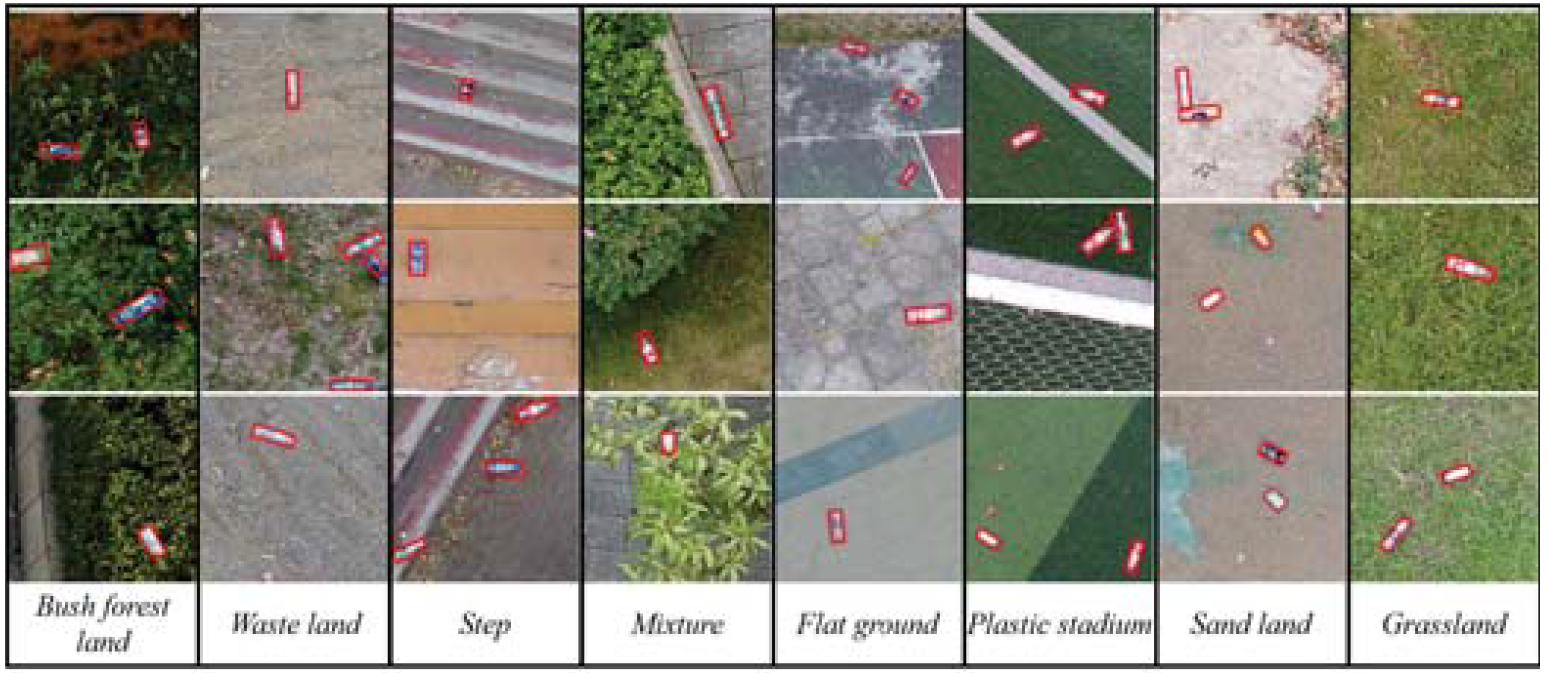
\includegraphics[width=0.9\linewidth]{BDWDataset1.png}
    \caption{Showcasing the different backgrounds found in the BDW dataset. (Source: \cite{bdwdataset})}
    \label{fig:bdw}
\end{figure}

The BDW dataset contains 25,407 annotated images with 34,791 object instances, all belonging to a single category: \textit{plastic bottles}. Annotations in the BDW dataset utilise \gls{obbs}, which include traditional bounding box coordinates along with additional parameters: centre coordinates ($c_x$, $c_y$), height ($h$), width ($w$), and orientation angle ($\theta$), where $\theta$ represents the angle from the horizontal axis. Additionally, the dataset was split randomly into training (64\%), validation (16\%), and testing (20\%) subsets \cite{bdwdataset}.

In their study, the authors utilise the created BDW dataset in multiple experiments to train object detection models, including Faster \gls{rcnn}, \gls{ssd}, \gls{yolo}v2, and a Modified \gls{rrpn} from \cite{rrpn}. Among these models, RRPN uniquely predicts OBBs, whereas the others predict standard axis-aligned bounding boxes. Wang et al. report that these experiments demonstrate that OBB regression is crucial for oriented object detection. In addition, RRPN achieved superior localisation accuracy while minimising false alarms and false positives, making it the most effective model in the study \cite{bdwdataset}.

\subsection{UM Geo. Survey}
\label{subsec:3_geosurvey}

Building on the concept of litter detection proposed by \cite{bdwdataset}, A. Deidun et al. (2018) introduced an optimised system for monitoring beach litter through aerial imagery \cite{umgeosurvey}. Their study focused on three coastal stretches within the North-East Marine Protected Area of the Maltese Islands. The monitored areas included Bahar Ic-Caghaq, which encompassed a rocky peninsula's western and eastern flanks, and Qawra Point. 
The data collection process utilised a DJI Phantom 4 Pro drone, configured with a gimbal angle of -90 degrees and flown at an \gls{agl} altitude of 30 metres. This altitude was empirically determined to balance image quality and spatial resolution, following tests conducted at heights ranging from 20 to 50 metres. Images were captured at varying ground resolutions, ranging from 2.5 to 50 centimetres per pixel, to provide detailed visual data \cite{umgeosurvey}.

The collected footage was processed using OpenDroneMap software \cite{OpenDroneMap}, which facilitated the creation of point clouds and texture maps. Georeferenced orthophoto maps with a resolution of 1 centimetre per pixel were generated using \gls{gps} metadata embedded in the \gls{exif} data of each image file. These orthophotos were subsequently tiled and visualised in Google Earth© \cite{umgeosurvey}.

\begin{figure}[!htbp]
    \centering
    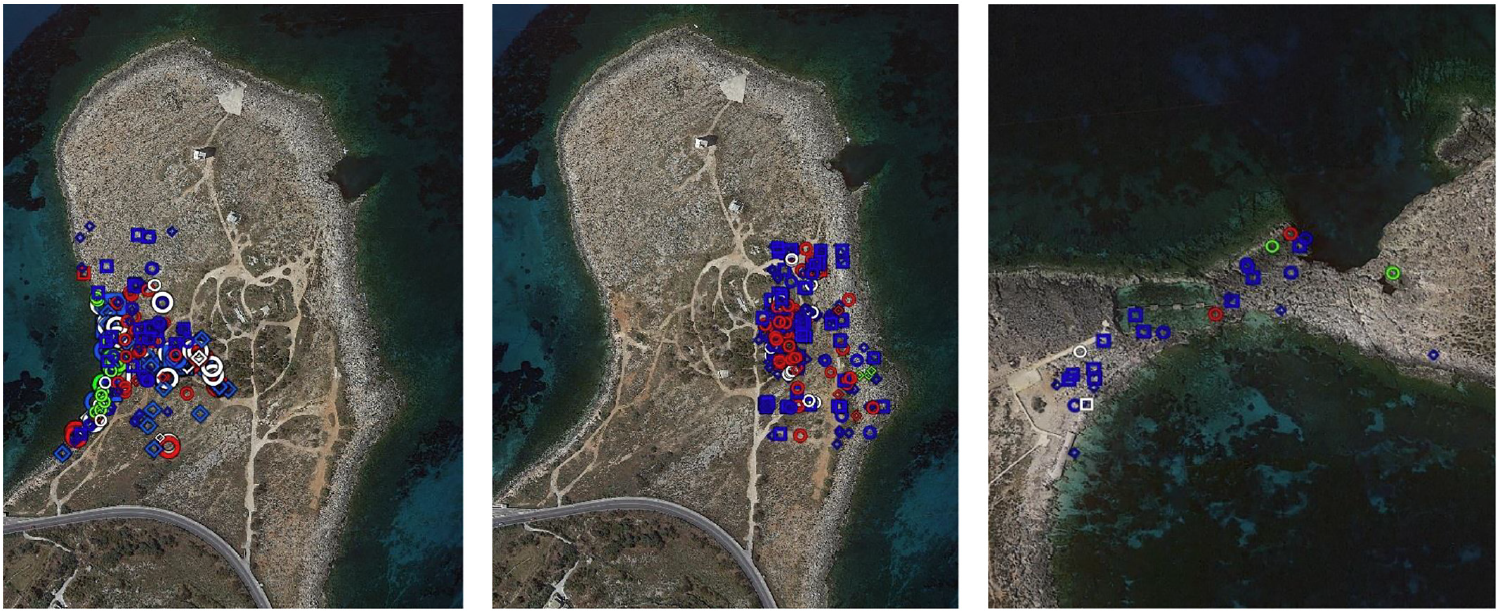
\includegraphics[width=1\linewidth]{UMgeosurvey.png}
    \caption{Showcasing snapshots from the digitised marine litter database, highlighting litter detected in the west (left) and east (middle) bays of Baħar iċ-Ċagħaq, and Qawra Point (right). Legend: blue = plastics; green = rope; red = wood; black = rubber; white = other non-natural materials. (Source: \cite{umgeosurvey})}
    \label{fig:geosurvey}
\end{figure}

The digitised database of detected marine litter, shown in Figure \ref{fig:geosurvey}, was created using 473 annotated images containing 608 labelled instances of litter. These instances were categorised into five types: \textit{plastics, rope, wood, rubber, and non-natural items}. While the study did not involve testing object detection algorithms, its key contribution lies in presenting a robust data collection protocol \cite{umgeosurvey}.

\subsection{SuperDock}
\label{subsec:3_superdock}

To address the environmental issue of trash in rivers, G. Niu et al. (2019) proposed an automated river trash monitoring system called SuperDock \cite{superdock}. This system consists of a \gls{rpu}, a docking station, and a \gls{uav}. SuperDock enables the UAV to land precisely on the docking station, where automated battery replacement is performed. This allows the UAV to resume its monitoring tasks without significant wasted time. SuperDock incorporates a deep learning-based trash detection module, leveraging the \gls{yolo}v3 architecture. As illustrated in Figure \ref{fig:superdock}, the system includes three key components: the RPU, the docking station, and the UAV. The object detection process uses data collected from a consumer-grade UAV flying at an \gls{agl} altitude of 5 to 10 meters \cite{superdock}.

\begin{figure}[!htbp]
    \centering
    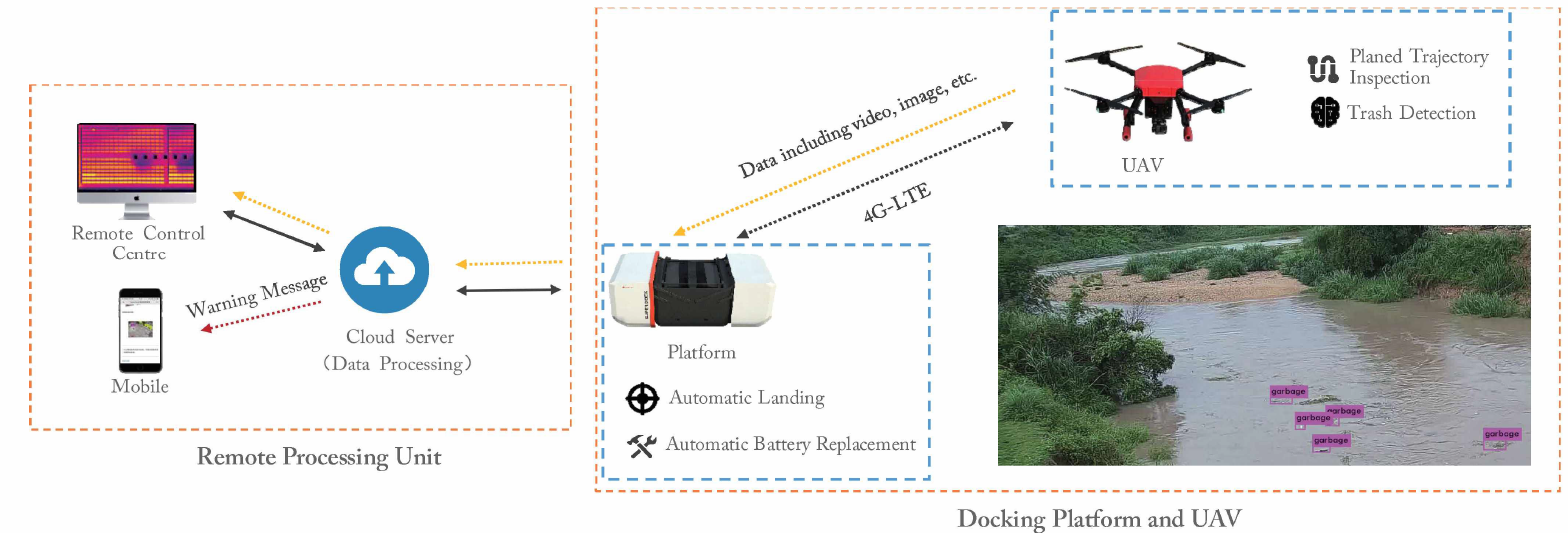
\includegraphics[width=0.9\linewidth]{superdock.png}
    \caption{Block diagram of the automated SuperDock system. (Source: \cite{superdock})}
    \label{fig:superdock}
\end{figure}

The dataset features 100 annotated images, divided into 80\% for training and 20\% for testing, with a total of 312 object instances. All types of litter in the dataset are annotated under a single category: \textit{garbage}. Data augmentation techniques were applied, increasing the dataset size by a factor of five. Additionally, the authors used Microsoft AirSim (Aerial Informatics and Robotics Simulation) to experiment with the gathered data. The dataset was used to train and test three models: Faster \gls{rcnn}, \gls{yolo}v3, and \gls{yolo}v3 with an improved loss function. Among these, the improved \gls{yolo}v3 model demonstrated the best performance in terms of both accuracy and processing time. While the study did not focus on creating a specialised litter detection dataset, its primary contribution lies in developing an automated trash monitoring system \cite{superdock}.

\subsection{Styrofoam Monitoring}
\label{subsec:3_styrofoam}
To analyse the patterns of waste generation and distribution, as well as the factors contributing to its inflow, S. H. Bak et al. (2019) proposed an automated floating trash monitoring system based on deep learning \cite{styrofoam}. Their study focused on Heungnam Beach in Geoje, situated in Korea’s marine climate zone on the South Sea. The system utilises SegNet \cite{segnet}, an instance segmentation model based on a convolutional encoder-decoder structure developed by the University of Cambridge, to detect beach litter.
While the authors did not specify the exact number of annotated images in the dataset, UAV imagery was collected using DJI's MAVIC 2 PRO, a multi-rotor UAV. The UAV operated at an altitude of 15 meters, chosen to account for the size of the beach litter and the \gls{gsd}. Orthoimages were generated using Pix4D and divided into $224 \times 224$-pixel segments for neural network input, with positional information recorded for each segment \cite{styrofoam}.

\begin{figure}[!htbp]
    \centering
    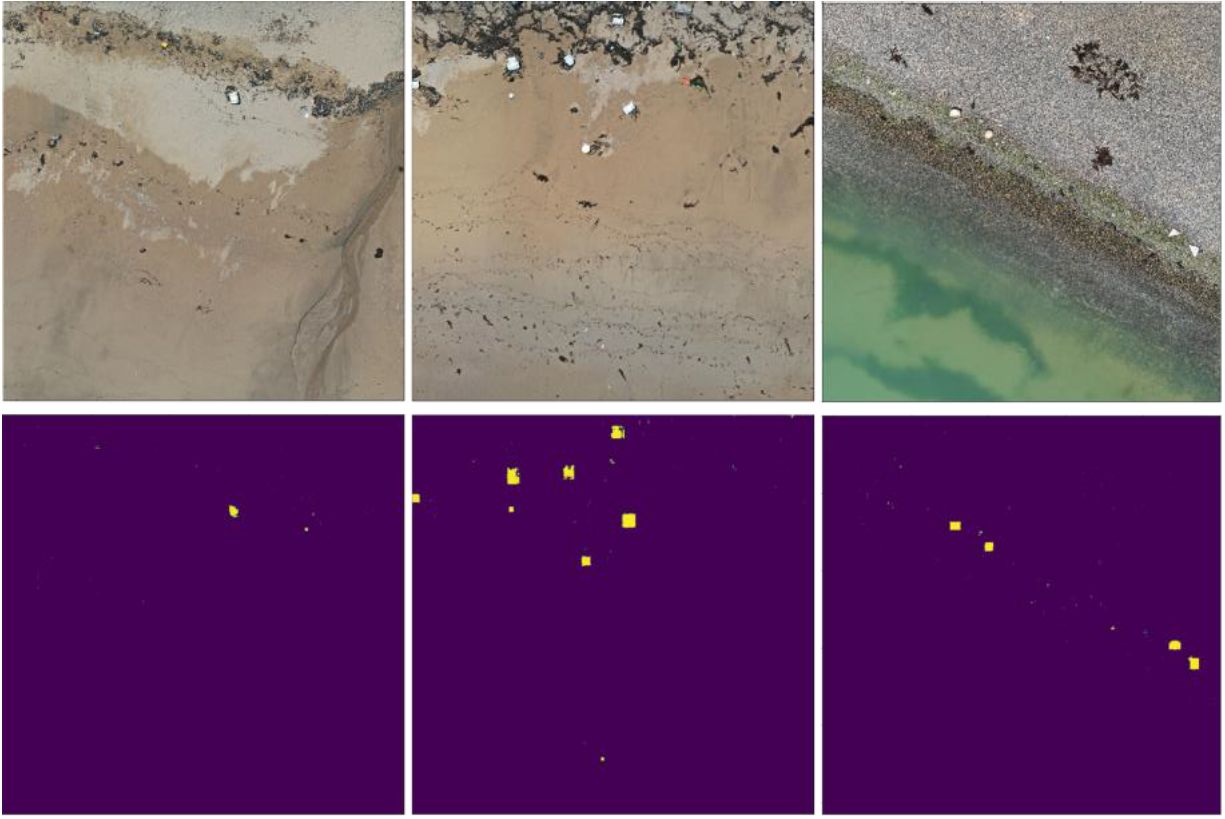
\includegraphics[width=0.7\linewidth]{styrofoam.png}
    \caption{Styrofoam detection results using the trained neural network. (Source: \cite{styrofoam})}
    \label{fig:styrofoam}
\end{figure}

The developed dataset only contained a single litter category, focusing on detecting \textit{Styrofoam} waste, and was notably imbalanced, as the majority of pixels represented the background, with less than 5\% occupied by detected objects. To mitigate this imbalance, data augmentation techniques were employed. Despite these challenges, the system achieved an impressive detection accuracy of 98.2\%, demonstrating its efficacy in identifying Styrofoam litter on beaches, as depicted in Figure \ref{fig:styrofoam} \cite{styrofoam}.

\subsection{Small Litter Detection}
\label{subsec:3_smalldetection}

In 2019, M. Schembri and D. Seychell proposed a case study focusing on litter detection through aerial imagery to address challenges in small object detection in highly variable backgrounds \cite{small_litter_detection}. This study explored techniques for small object localisation using \gls{cnn} to detect litter in outdoor, non-urban imagery. The dataset for this research was collected using a consumer-grade UAVs at altitudes ranging from 5 to 10 metres \gls{agl}. Compiled from land surveys conducted within the Maltese Islands, the dataset includes 744 annotated images with all types of litter objects classified under a single \textit{litter} category \cite{small_litter_detection}.

The authors proposed an algorithmic pipeline for small litter detection, as illustrated in Figure \ref{fig:smalllitterdetection}. A sliding window technique was used to subdivide the entire scene into tiles of $224 \times 224$ pixels with a 32-pixel overlap, and each tile was processed individually. Non-relevant objects such as the sky, sea, and humans were masked during a scene filtering stage to enhance accuracy. The litter detection problem was tackled using a VGG-16 CNN model, pre-trained on ImageNet, and fine-tuned with the collected dataset. Data augmentation techniques were also applied to improve the model’s robustness \cite{small_litter_detection}.

\begin{figure}[!htbp]
    \centering
    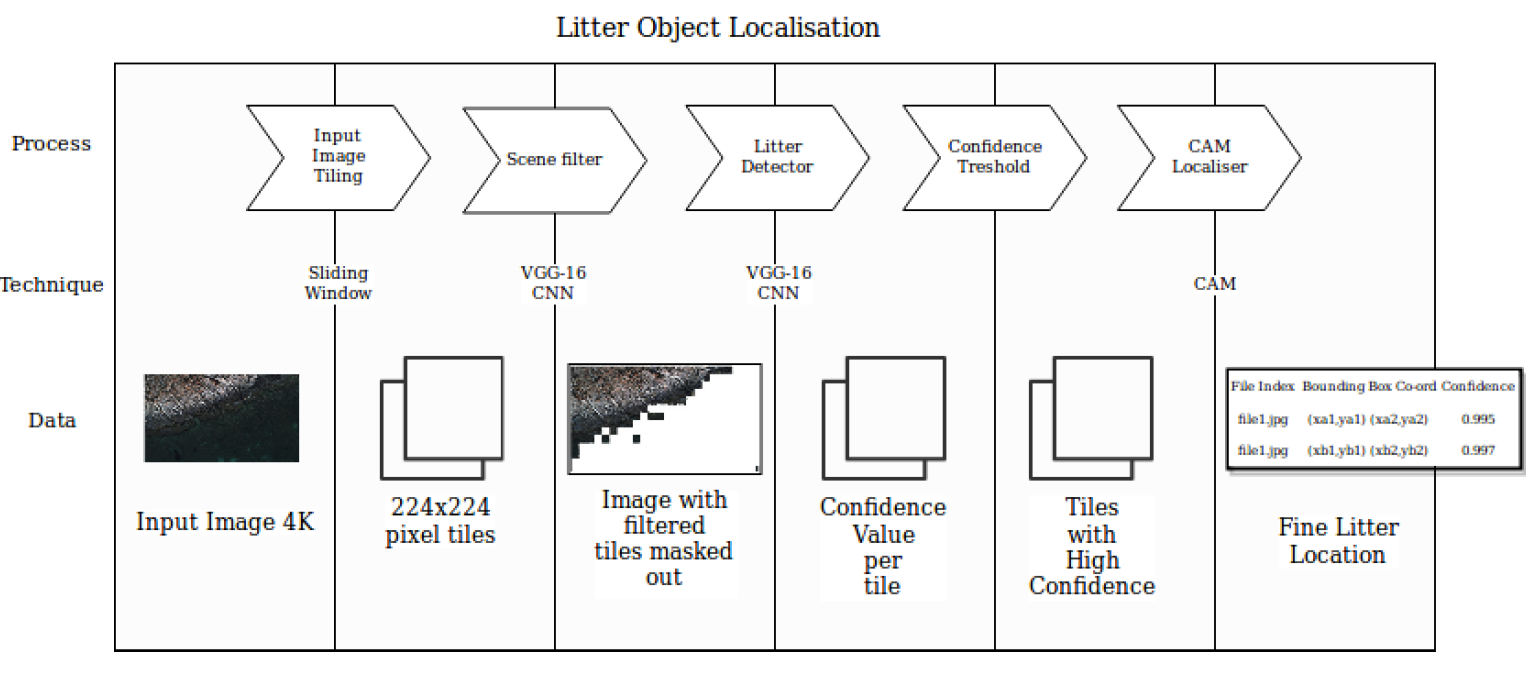
\includegraphics[width=0.9\linewidth]{small_litter_detection.png}
    \caption{Data flow and process diagram of the litter detection algorithm. (Source: \cite{small_litter_detection})}
    \label{fig:smalllitterdetection}
\end{figure}

Due to the dataset’s foreground-to-background sample ratio of 1:20, a confidence threshold was used to refine the detection results. \gls{cam} was employed to improve the \gls{iou} score by highlighting relevant foreground areas. Thresholding and normalising the heatmap allowed for generating masks that effectively located the target objects. An IoU threshold of 0.01 for \gls{nms} was used to facilitate the detection of very small objects.
The study identified that stones and vegetation were among the classes frequently misclassified as litter. To address this issue, the authors proposed a two-stage model incorporating a terrain filter to automate the detection of misclassifications, which provided improved results. They also concluded that litter with more defined shapes was easier to detect for both human annotation and algorithmic detection. 
The authors also trained Faster \gls{rcnn} on the same dataset and observed lower performance metrics, which were attributed to its difficulty in handling highly variable background representations \cite{small_litter_detection}.

\subsection{TACO Dataset}
\label{subsec:3_tacodataset}

Detecting litter in natural environments presents considerable challenges due to the variability of litter, which can be deformable, transparent, aged, fragmented, occluded, and camouflaged. Additionally, models must contend with the wide variety of features found in natural landscapes. To tackle these issues, P. F. Proença and P. Simões introduced the \gls{taco} dataset in 2020 \cite{taco2020}. This dataset was created to feature images captured from a variety of global environments, as shown in Figure \ref{fig:taco1}, including beaches and urban areas, with litter segmented and annotated according to a hierarchical classification system \cite{taco2020}.

\begin{figure}[!htbp]
    \centering
    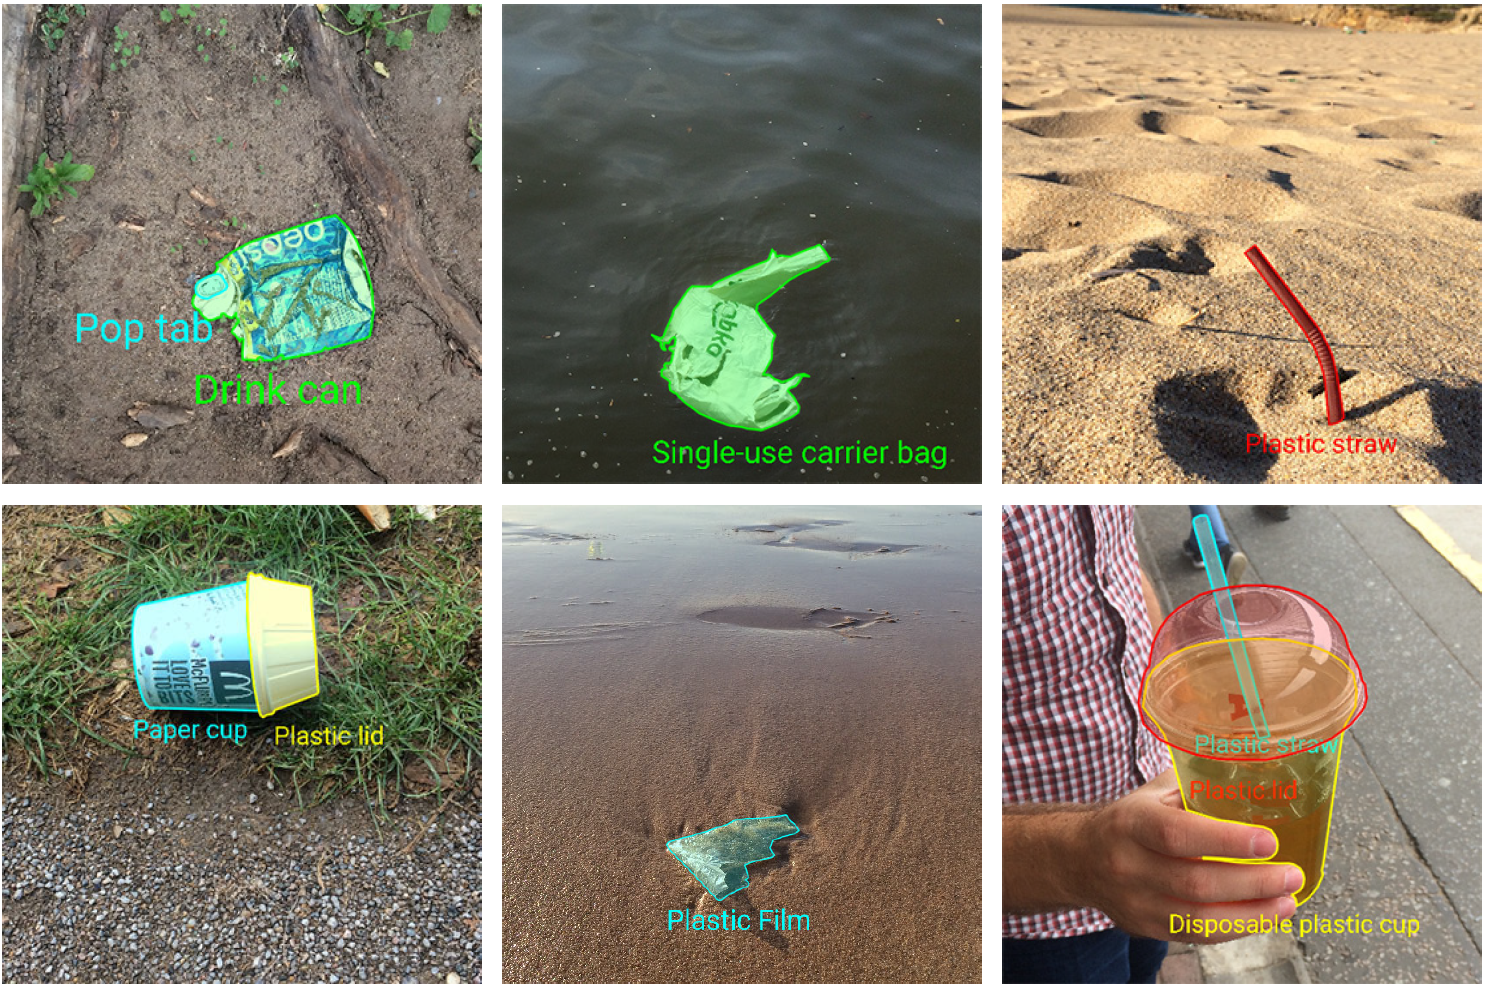
\includegraphics[width=0.8\linewidth]{taco1.png}
    \caption{Annotated images from the \gls{taco} dataset, with litter objects marked using polygon masks for instance segmentation. (Source: \cite{taco2020})}
    \label{fig:taco1}
\end{figure}

The \gls{taco} dataset includes 60 distinct litter categories, organised into 28 top-level categories, as observed in Figure \ref{fig:taco2}. Unlike UAV-based datasets, \gls{taco} consists of images captured from ground-level natural environments. At the time of release, the dataset comprised 1,500 annotated images and 4,784 instances of litter, with an additional 3,918 new images currently awaiting annotation. The dataset uses polygon masks for annotation in an attempt to tackle the problem of instance segmentation \cite{taco2020}.
The authors conducted several experiments using Mask \gls{rcnn} to evaluate the dataset's performance. Two configurations were tested:
\begin{itemize}
    \item \textbf{\gls{taco}-1:} Identifying a single class of litter.
    \item \textbf{\gls{taco}-10:} Identifying ten distinct litter classes.
\end{itemize}

\begin{figure}[ht]
    \centering
    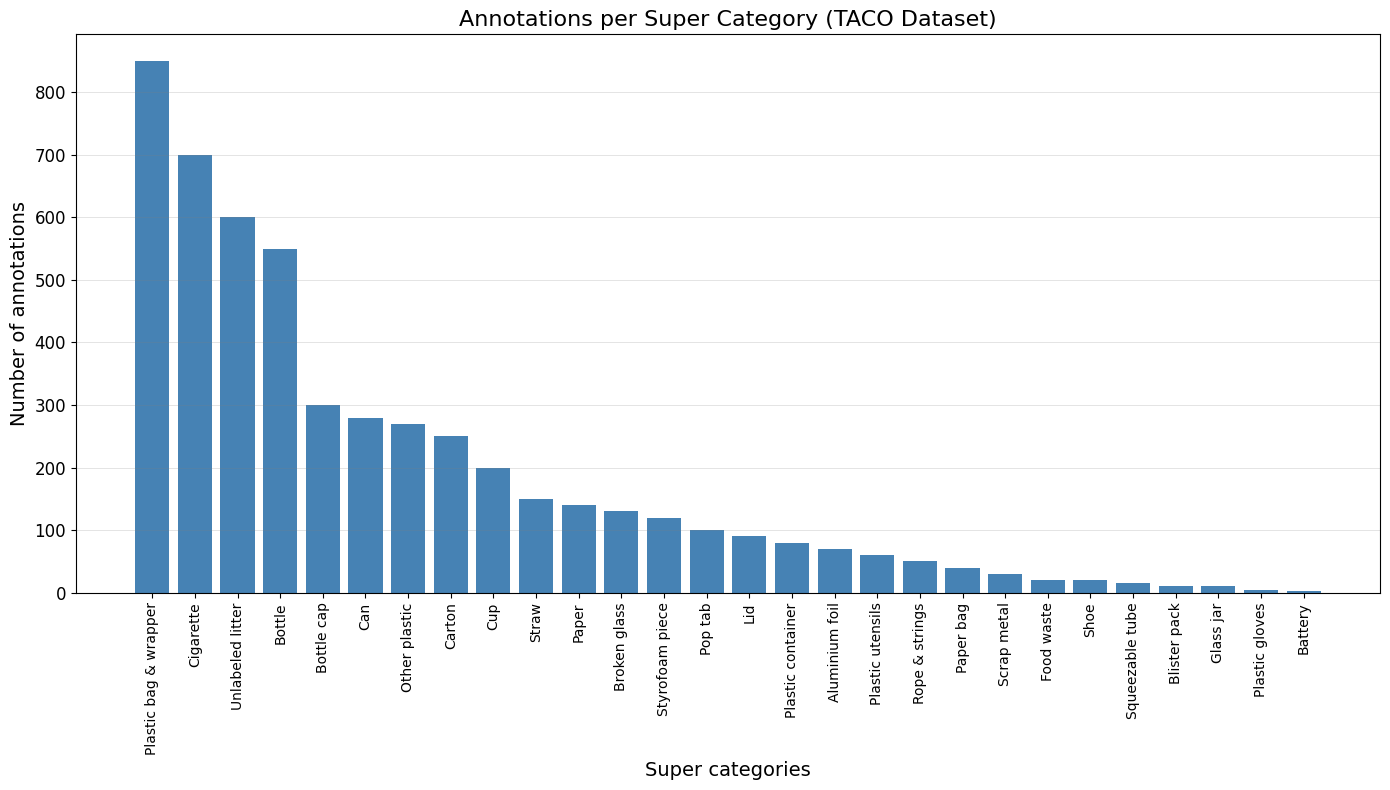
\includegraphics[width=0.7\linewidth]{taco2.png}
    \caption{Number of annotations per super category in the published version of the \gls{taco} dataset. (Source: \cite{taco2020})}
    \label{fig:taco2}
\end{figure}

The authors noted that the detection performance was notably low due to challenges in detecting small items, particularly cigarette butts, which led to a high rate of false positives and negatives. This was attributed to their small size, with most images resized to $1024 \times 1024$ pixels, causing many small objects (less than $20 \times 20$ pixels) to be missed. Larger objects, such as cans and bottles, were detected more accurately, though a considerable number of bottles were misclassified as cans. Confusion was also observed between \textit{plastic bags} and \textit{other litter}, which is understandable given the material similarities between these categories \cite{taco2020}.

\subsection{MJU-Waste Dataset}
\label{subsec:3_mju-waste}

In 2020, T. Wang et al. also sought to address the challenge of waste object segmentation through a multi-level approach \cite{mju_waste}. To create their dataset, the authors collected waste items from a university campus, photographed individuals holding these items, and then annotated the images. The MJU-Waste dataset focuses solely on a single category, classifying all items under the label of \textit{waste}. The MJU-Waste dataset contains 2,475 annotated images and 2,525 instances of litter, all of which are annotated using polygon masks.
Unlike UAV-based datasets, the MJU-Waste dataset consists of images captured from controlled environments. The dataset includes segmentation masks, along with both raw and processed depth maps for all litter instances, captured using a Microsoft Kinect RGBD camera. However, due to sensor limitations, the depth frames contain missing values, particularly at reflective surfaces, occlusion boundaries, and distant regions. To address this, a median filter was applied to fill in the missing data and ensure the depth images were of high quality. Each image in the dataset was annotated with pixel-wise masks of the waste objects, and examples of colour frames, ground-truth annotations, and depth frames are provided in Figure \ref{fig:mjuwaste}. Alongside the semantic segmentation ground truths, object instance masks are also available \cite{mju_waste}.

\begin{figure}[!htbp]
    \centering
    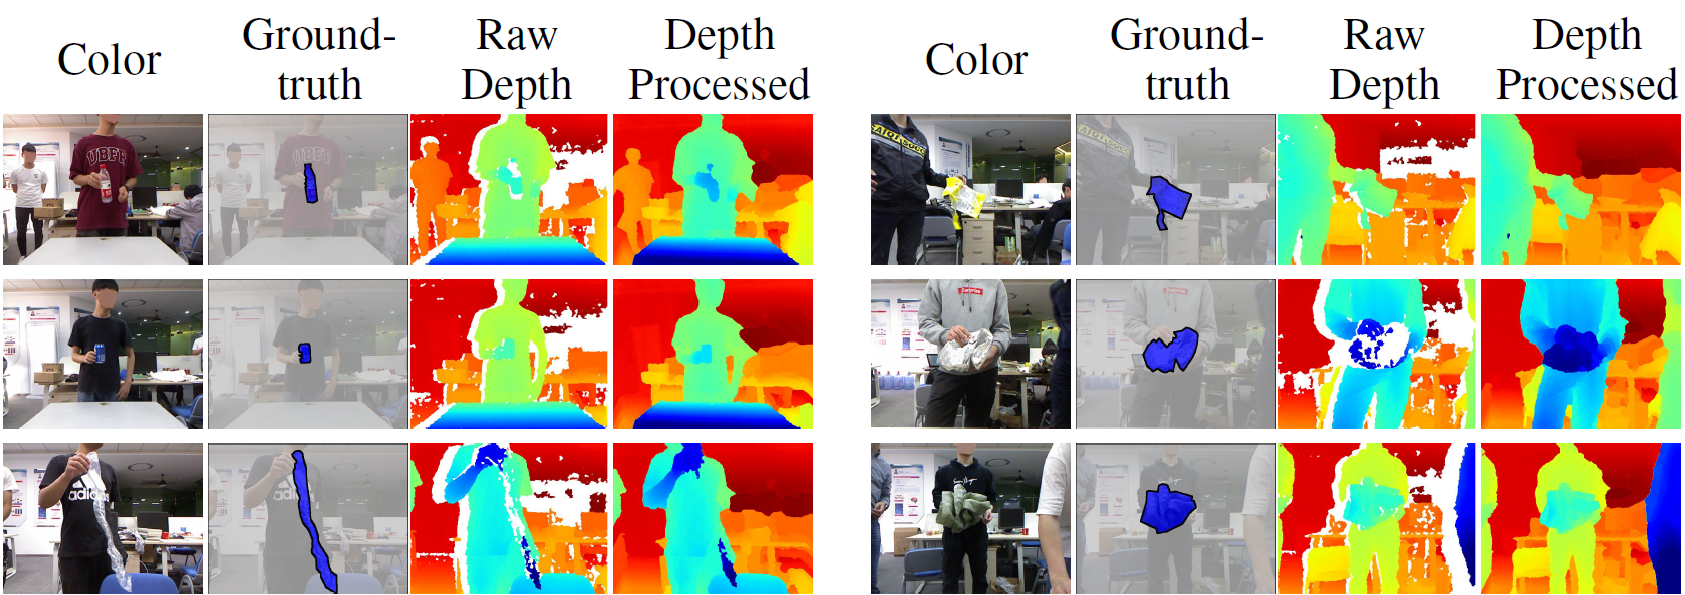
\includegraphics[width=1\linewidth]{mjuwaste.png}
    \caption{Sample RGB images, ground-truth annotations, and depth frames from the MJU-Waste dataset. (Source: \cite{mju_waste})}
    \label{fig:mjuwaste}
\end{figure}

The authors evaluate their proposed method against state-of-the-art semantic segmentation baselines. Their approach adopts a multi-level strategy for waste object segmentation, involving three key stages: first, scene-level parsing for initial coarse segmentation; second, object-level parsing to refine object region proposals; and third, pixel-level refinement using colour, depth, and spatial affinities. By combining inference from all three levels, the method achieves a coherent and accurate final segmentation.
In addition, the study focuses on two particularly challenging scenarios for waste object localisation: the hand-held setting, which is crucial for applications such as service robot interactions and smart trash bins, and waste objects found in natural environments. A significant challenge noted by the authors in both cases is the extreme variation in object scale, which leads to suboptimal performance from standard segmentation algorithms \cite{mju_waste}.

In comparison to the \gls{taco} dataset, the MJU-Waste dataset is split as follows: 60\% for training, 10\% for validation, and 30\% for testing. The evaluation metrics used include \gls{iou}, mean \gls{iou}, and pixel precision. The models tested include FCN-8s \cite{fcn}, PSPNet \cite{pspnet}, CCNet \cite{ccnet}, and DeepLabv3 \cite{deeplabv3}. Among these, DeepLabv3 performed best in terms of IoU and mIoU, while CCNet excelled in pixel precision. Notably, DeepLabv3 also outperformed other models when tested on the \gls{taco} dataset.
The authors also conclude that their multi-level approach proved effective, with scene-level segmentation, object-level segmentation, and pixel-level refinement working together to produce high-quality localisation results \cite{mju_waste}.

\subsection{UAVVaste}
\label{subsec:3_uavvaste}

In 2021, M. Kraft et al. addressed the challenge of detecting litter and the associated issue of mapping detected litter geographically \cite{uavvaste}. Their proposed system employed a \gls{uav} equipped with onboard sensors to process low-altitude aerial imagery. A key feature of the system was its reliance on low-cost, commercially available components, which were integrated into a self-contained solution capable of autonomous operation during UAV patrol missions.
A notable contribution of their research was the introduction of an application-specific dataset, UAVVaste. This dataset consists of 772 images with 3,716 bounding box annotations, as illustrated in Figure \ref{fig:uavvaste1}, and is dedicated to a single category: litter, labelled as \textit{rubbish}. The creation of this dataset was motivated by the lack of domain-specific data tailored to UAV-based litter detection. Compared to the \gls{taco} dataset, the UAVVaste dataset features a marked distribution shift, characterised by smaller object sizes, reflecting the unique challenges of detecting litter in aerial imagery \cite{uavvaste}.

\begin{figure}[!htbp]
    \centering
    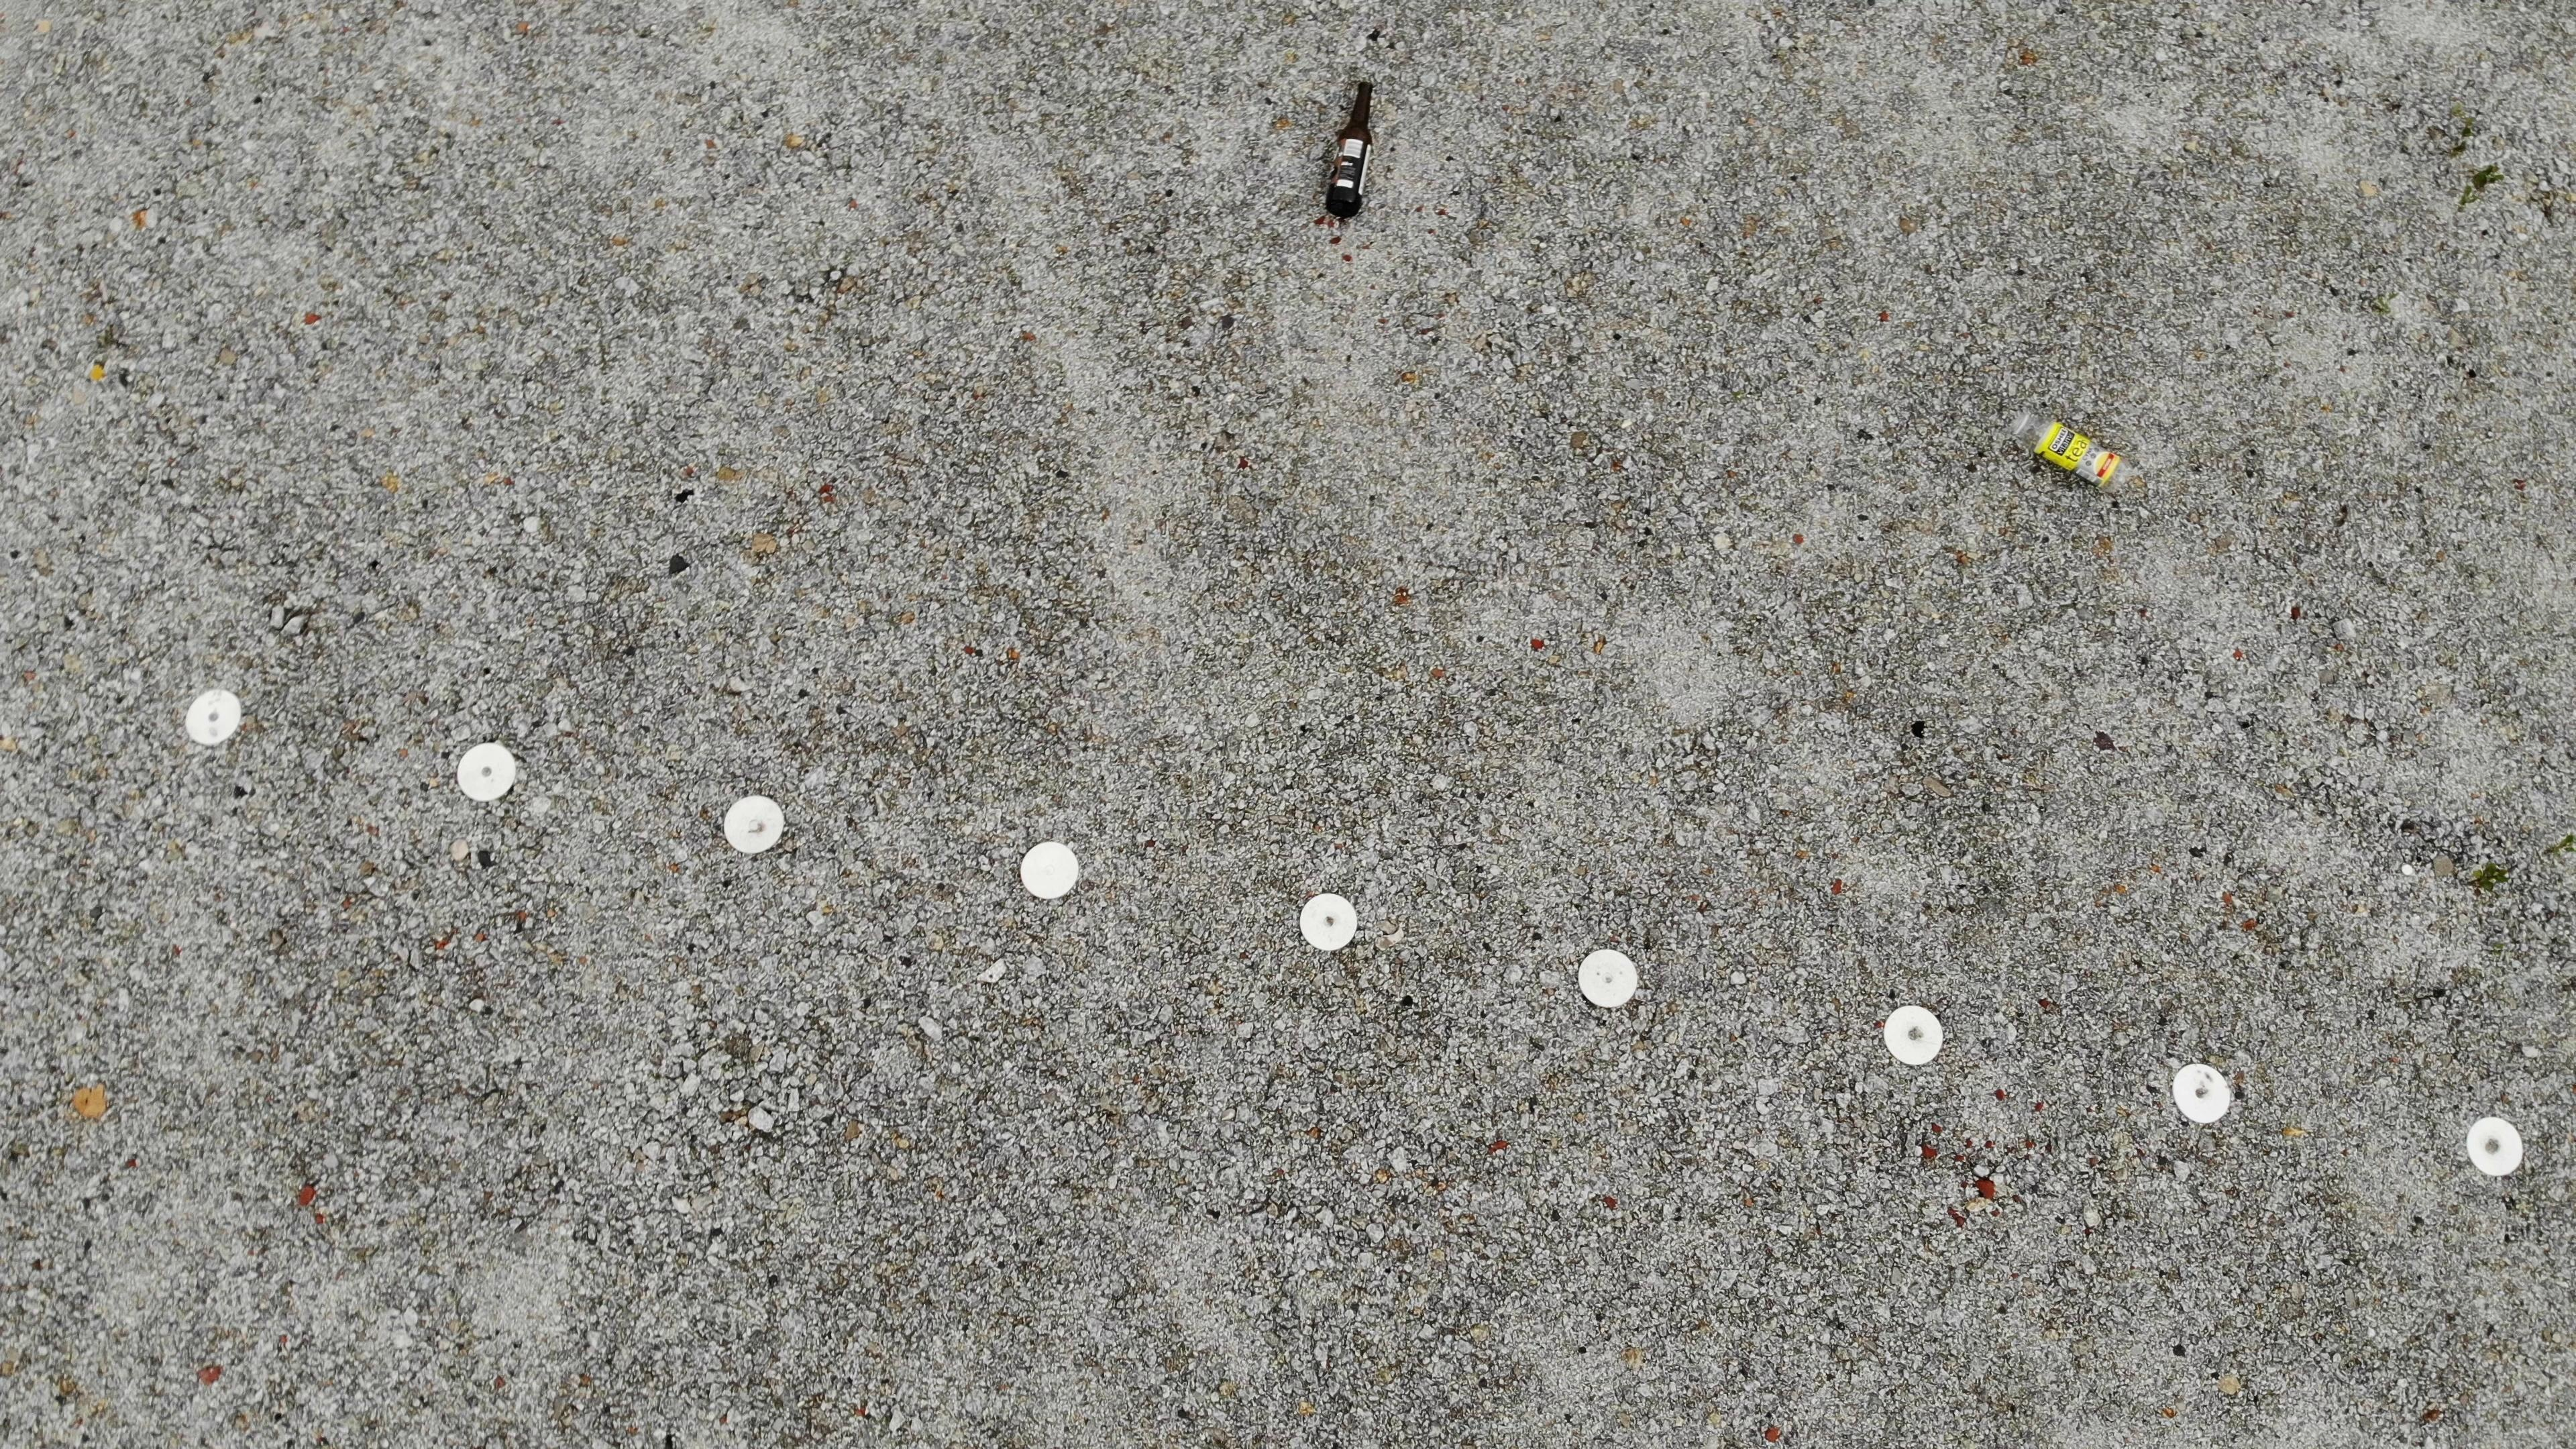
\includegraphics[width=0.9\linewidth]{uavvaste1.png}
    \caption{Sample images from the UAVVaste dataset with litter objects annotated using bounding boxes. (Source: \cite{uavvaste})}
    \label{fig:uavvaste1}
\end{figure}

The UAV hardware used in the study included a Pixhawk 2 autopilot controller, a Here2 \gls{gps}/\gls{gnss} module equipped with a barometric pressure sensor, and a downward-facing camera stabilised using a gimbal. The computational platform featured multiple components, including an Nvidia Xavier NX, a Google Coral USB (\gls{tpu}), and a Raspberry Pi 4. A variety of neural network architectures were evaluated for litter detection. These included \gls{ssd} detectors with lightweight backends optimised for TensorFlow Lite, which operated efficiently on the Google Coral TPU, as well as \gls{yolo}v3 and \gls{yolo}v4 and their lightweight variants. For models deployed on the Nvidia Xavier NX, TensorRT was utilised to optimise performance. Additionally, EfficientDet with a MobileNet backend was implemented. Training these models involved transfer learning, leveraging pre-trained weights from the \gls{coco} dataset to improve performance \cite{uavvaste}.

\begin{figure}[!htbp]
    \centering
    \includegraphics[width=0.9\linewidth]{uavvaste2.png}
    \caption{A schematic representation of the camera setup and acquired image, along with the key parameters. (Source: \cite{uavvaste})}
    \label{fig:uavvaste2}
\end{figure}

A significant portion of the study focused on the geolocation algorithm, which marks detected litter objects on a map using the UAV’s onboard sensors. This process required camera calibration, performed using the Kalibr library, and lens distortion correction, ensuring accurate geometric relationships between the image and real-world coordinates. The algorithm assumed a vertical downward orientation for the camera during operation. Using the known viewing angles of the camera and the UAV’s altitude, the algorithm calculated the size of the area captured in each image. Figure \ref{fig:uavvaste2} provides a schematic representation of the camera setup and the acquired image, highlighting the key parameters involved in the process. While the camera parameters were determined with high precision, the accuracy of object localisation on the map was predominantly influenced by the accuracy of altitude measurements. The authors observed that any error in altitude measurement would proportionally affect the localisation accuracy.
The evaluation metrics used in the study included the \gls{map} scores from the \gls{coco} dataset, calculated at \gls{iou} thresholds of 0.5 and 0.95. Separate \gls{map} and recall scores were also reported for small, medium, and large objects. Among the models tested, \gls{yolo}v4 achieved the highest \gls{map}, while EfficientDet excelled in recall, particularly for smaller objects \cite{uavvaste}.

\subsection{ZeroWaste Dataset}
\label{subsec:3_zerowaste}

In 2022, D. Bashkirova et al. introduced the first industrial-grade, in-the-wild waste detection and segmentation dataset, ZeroWaste, making a significant contribution to computer-aided waste detection \cite{zerowaste}. The dataset features four categories of litter: \textit{cardboard}, \textit{soft plastic}, \textit{rigid plastic}, and \textit{metal}. Unlike UAV-based datasets, the images in ZeroWaste were captured in real-world settings.
The ZeroWaste dataset includes 10,715 annotated images, collected from a high-quality paper conveyor at a single-stream recycling facility in Massachusetts, containing 27,744 instances of litter, all annotated in polygon format, as illustrated in Figure \ref{fig:zerowaste}. Data augmentation was also applied to the dataset to improve model generalisation by artificially increasing the variety of training samples. Furthermore, this four-class labelled dataset captures various waste items identified during the sorting process at the facility, which aims to separate high-quality paper from contaminants such as metal, plastic, brown paper, and cardboard \cite{zerowaste}.

\begin{figure}[!htbp]
    \centering
    \includegraphics[width=0.9\linewidth]{zerowaste.png}
    \caption{Sample images (left) and ground truth polygon annotations (right) in the ZeroWaste dataset. (Source: \cite{zerowaste})}
    \label{fig:zerowaste}
\end{figure}

The data was gathered using two compact recording systems placed at the start and end of the conveyor belt during the facility's routine operations. The footage consists of 12 video sequences with a total duration of 95 minutes and 14 seconds, recorded at a frame rate of 120 FPS and a resolution of $1920 \times 1080$. To ensure high-quality data, the footage was processed to correct optical distortions, crop unnecessary elements, and remove motion blur.
The ZeroWaste dataset was divided as follows: 65\% for training, 15\% for validation, and 20\% for testing. The evaluation metrics used include \gls{ap} and \gls{map} at various thresholds, \gls{iou}, and pixel precision. The models tested include RetinaNet, Mask \gls{rcnn}, TridentNet \cite{tridentnet}, and DeepLabv3, and a series of experiments were conducted, including fully, semi, and weakly supervised learning.
The results revealed that the ZeroWaste dataset posed considerable challenges for state-of-the-art detectors like Mask \gls{rcnn}. However, TridentNet emerged as the top-performing detector, while DeepLabv3 achieved the best results in terms of segmentation \cite{zerowaste}.

\subsection{PlastOPol Dataset}
\label{subsec:3_plastopol}

To address the issue of litter accumulation, M. Córdova et al. investigated the effectiveness of lightweight neural networks for detecting litter in real-world environments with complex and crowded image backgrounds \cite{plastopol}. The study also evaluated the feasibility of deploying these models on mobile devices with limited memory capacity (hereafter referred to as efficiency). Their 2022 publication presented two key contributions: a comparative analysis of state-of-the-art deep learning techniques for image-based litter and waste detection and the introduction of a novel dataset, PlastOPol, comprising 2,418 images captured in real-world conditions with 5,300 litter annotations.
The PlastOPol dataset includes a single class, with all litter items categorised under the label \textit{litter}. The dataset consists of images from natural settings rather than being derived from \gls{uav} data. These images were sourced using the Marine Debris Tracker and are publicly available under a Creative Commons Attribution licence. The dataset was annotated in a bounding box format and focused on the problem of object detection. Of the 5,300 annotated instances, 90.98\% are large objects, 8.40\% are medium objects, and only 0.62\% are small objects \cite{plastopol}.

\begin{figure}[!htbp]
    \centering
    \includegraphics[width=1\linewidth]{plastopol.png}
    \caption{Visual detection results on the PlastOPol dataset. (Source: \cite{plastopol})}
    \label{fig:plastopol}
\end{figure}

To assess the performance of various deep learning models in detecting litter, the authors used both the proposed PlastOPol dataset and the publicly available \gls{taco} dataset. For the PlastOPol dataset, the data was split into 80\% for training and 20\% for testing. Evaluation metrics included \gls{ap}, \gls{map} at \gls{iou} threshold 0.5, F1-score, and recall. The models tested included EfficientDet, Faster \gls{rcnn}, Mask \gls{rcnn}, RetinaNet, and \gls{yolo}v5. As shown in Figure \ref{fig:plastopol}, the visual detection results on the PlastOPol dataset highlight the performance of these models in identifying litter objects across different environments.
The experiment results demonstrated that \gls{yolo}v5 was the best-performing model overall. The authors also observed that \gls{yolo}v5 and EfficientDet were the fastest models, even when deployed on mobile devices. However, they noted that all methods struggled with detecting small objects, such as cigarette butts. Furthermore, \gls{yolo}v5x outperformed Faster \gls{rcnn} and Mask \gls{rcnn} in terms of speed \cite{plastopol}.

\subsection{HAIDA Dataset}
\label{subsec:3_haida}

In 2022, Y.-H. Liao and J.-G. Juang developed a marine trash detection system using \gls{uav}s, aiming to replace manual efforts with UAVs for efficient marine trash detection and to provide real-time information on pollution to government agencies \cite{haida}. The real-time UAV trash monitoring system consisted of nine components: UAVs, a message queuing system, a database, a video streaming server, a connector, a UAV control station, a web service, a UAV map, and a data analysis module, as illustrated in Figure \ref{fig:haida1}. The ground station incorporated key elements, such as the video streaming server, Kafka, the Kafka connector, MongoDB, and the web service. The system addressed two key challenges: object detection and geolocation, and as part of the system's development, the authors introduced the HAIDA dataset. This dataset, collected on the NTOU campus, was used to train the object detection model and contains two types of litter objects: \textit{garbage} and \textit{bottles}. The data was gathered using a UAV equipped with a Pixhawk controller and an NVIDIA Jetson Xavier NX. The UAV operated at altitudes ranging from 1 to 10 metres \gls{agl} \cite{haida}.

\begin{figure}[!htbp]
    \centering
    \includegraphics[width=0.7\linewidth]{haida1.png}
    \caption{The system architecture of the real-time \gls{uav} trash monitoring system. (Source: \cite{haida})}
    \label{fig:haida1}
\end{figure}

The HAIDA dataset comprises 1,319 annotated images, with 6,475 instances of litter, including 3,904 garbage objects and 2,571 bottle objects. Additionally, 456 images in the dataset contain no litter. The authors utilised the dataset to train the \gls{yolo} object detection model (version unspecified). The results showed that the model was able to identify trash objects with an \gls{ap} of over 70\% at a 0.5 \gls{iou} threshold. Notably, as shown in Figure \ref{fig:haida2}, the detection confidence for small objects was high, with confidence scores of 98.27\%, 64.65\%, and 91.86\% for different categories of litter.
The real-time UAV trash monitoring system operated by first collecting UAV footage as the drone flew across predetermined waypoints. The footage was then transmitted to a server via Kafka, where it was stored in an online database such as Oracle, MySQL, or MongoDB. Using this stored data, the server applied the trash detection model to identify litter both in the images and on a map. Control stations, both mobile and desktop, could make requests to the server to retrieve the map data, which displayed the locations of detected litter \cite{haida}.

\begin{figure}[!htbp]
  \centering
  \begin{tabular}{cc}
    \includegraphics[width=0.48\textwidth, height=5cm]{haida2.png} &
    \includegraphics[width=0.48\textwidth, height=5cm]{haida3.png} \\
    \small (a) & \small (b) \\
  \end{tabular}\\
  \caption{\gls{uav} trash monitoring results on the NTOU campus. (a) Detection results from the UAV. (b) Detected litter plotted on a map, showing real-time monitoring and detection. (Source: \cite{haida})}
  \label{fig:haida2}
\end{figure}

To tackle the problem of litter geolocation, the authors adapted a similar approach to the one described in \cite{uavvaste}, enabling the calculation of the detected trash pollution area based on several factors. These factors include the camera’s horizontal and vertical angle of view, the UAV’s altitude, the camera's field of view, the dimensions of the camera's image, the size of the detected trash in the image, and the detected trash's area in both the image and the real-world environment. By incorporating these variables, the system can accurately estimate the location and extent of trash pollution in the area \cite{haida}.

\subsection{Bangladeshi Dataset}
\label{subsec:3_bangladeshi}

As populations in underdeveloped nations continue to grow, the challenges associated with trash production and disposal have become more urgent. Aware of the time-consuming and potentially hazardous nature of manual litter classification, D. Das et al. (2023) aimed to tackle this issue by developing automated methods for more efficient and safer waste management \cite{bangladeshi}. To achieve this, they focused on collecting data that accurately captured the complexities of litter in Bangladesh, creating an outdoor dataset, and incorporating OpenLitterMap to broaden its scope. This dataset comprises images from natural settings, not UAV-based data, and includes ten categories of litter: \textit{tissue paper}, \textit{plastic}, \textit{medical waste}, \textit{rope}, \textit{paper}, \textit{cigarette butts and boxes}, \textit{metal}, \textit{glass}, \textit{organic waste}, and \textit{textiles}. Initially consisting of 1,283 annotated images, the dataset was expanded to 4,418 by integrating data from OpenLitterMap, a global database containing litter and plastic images. The Bangladeshi dataset contains 6,178 instances of litter, which was extended to 8,077 while retaining the ten distinct classes \cite{bangladeshi}.

\begin{figure}[!htbp]
  \centering
  \begin{tabular}{c}
    \includegraphics[width=1\textwidth]{bangladeshi1.png} \\
    \small (a)\\
    \includegraphics[width=1\textwidth]{bangladeshi2.png} \\
    \small (b) \\
  \end{tabular}\\
  \caption{Litter detection results using different versions of the \gls{yolo}v5 model on the Bangladeshi dataset. (a) 2 instances of litter; (b) 17 instances of litter. (Source: \cite{bangladeshi})}
  \label{fig:bangladeshi}
\end{figure}

The experimental setup used for this study involved a comparison with the \gls{taco} and PlastOPol datasets. The Bangladeshi dataset was divided as follows: 80\% for training, 10\% for validation, and 10\% for testing. The evaluation metrics included \gls{ap} and \gls{map} at \gls{iou} thresholds from 0.5 to 0.95, as well as F1-measure and recall. Several models were tested, including different versions of \gls{yolo}v5, \gls{yolo}v6, \gls{yolo}v8, and Faster \gls{rcnn}. The authors also employed data augmentation techniques during training and optimised model performance by adjusting hyperparameters.
In their study, the authors reported that \gls{yolo}v5x was the best-performing model, as visually demonstrated in Figure \ref{fig:bangladeshi}, which shows a comparison of the detection bounding boxes on the images, demonstrating the improved \gls{map} for the expanded dataset. However, single-class detection experiments on the \gls{taco} and PlastOPol datasets yielded better results compared to the Bangladeshi dataset. D. Das et al. also highlighted that in future work, they plan to expand the dataset to include a broader range of categories, such as ocean waste, which is currently absent. Additionally, other object detection methods, such as \gls{ssd}, Mask \gls{rcnn}, and EfficientDet, could also be evaluated using their dataset \cite{bangladeshi}.

\subsection{Beach Litter Dataset}
\label{subsec:3_beach_litter}

In 2023, R. Pfeiffer et al. proposed a framework for an autonomous beach litter monitoring and retrieval system based on drone surveys and object detection using deep learning techniques \cite{beach_litter}. Their research combined drone footage collected from the islands of Malta and Gozo, Sicily (Italy), and the Red Sea coast with publicly available litter datasets, which were subsequently used to train an object detection model for identifying litter in the captured footage. Figure \ref{fig:beachlitter1} illustrates the overall framework of the proposed beach litter monitoring system. To address both object detection and geolocation challenges, the authors compiled a \gls{uav} dataset collected with DJI Phantom 4 Pro 2.0 and DJI Mavic 2 UAVs. The dataset covered altitudes ranging from 10 metres above ground level to 60 metres above sea level and included 67 types of litter, which were categorised into seven meta-classes: \textit{clothing \& fabric}, \textit{glass}, \textit{small objects}, \textit{metal litter}, \textit{paper \& cardboard}, \textit{plastic}, and \textit{other waste}.
Additionally, the Beach Litter Dataset contains 4,126 annotated images and 10,611 litter instances, including 1,154 images with no litter present. The dataset was divided as follows: 60\% for training, 20\% for validation, and 20\% for testing. The models were evaluated using metrics such as \gls{ap},\gls{map} (at 0.5–0.95), F1-measure, and recall, with the \gls{yolo}v5 model being the primary model used for training \cite{beach_litter}. 

\begin{figure}[!htbp]
    \centering
    \includegraphics[width=0.7\linewidth]{beachlitter1.png}
    \caption{The system architecture of the real-time \gls{uav} beach litter monitoring and geolocation system, highlighting the two main pipelines: training (in red) and prediction (in green). (Source: \cite{beach_litter})}
    \label{fig:beachlitter1}
\end{figure}

The authors also developed a geolocation algorithm to enhance the utility of the detected litter by integrating it with a robot for debris retrieval. For the algorithm to communicate the detection coordinates to the robot, the predictions made by the \gls{yolo}v5 model needed to be geolocated. This required that the original footage include \gls{gps} coordinates of the drone. The geolocation process involved several key steps: calculating the pixel size of the footage, determining the distance between meridians and parallels at the latitude of recording, measuring the horizontal and vertical distance from the prediction box's centre to the image centre, and transforming these distances into real-world coordinates. Figure \ref{fig:beachlitter2} shows the schematic for calculating litter geolocations, highlighting the parameters used to map the detected litter to real-world coordinates. To improve accuracy, the authors also calculated the distance between each litter object and the camera’s field of view, factoring in variables such as the \gls{uav}’s height and the angle of the camera’s lens. This enabled precise localisation of litter in both the image and the real-world environment, essential for guiding the robot to specific debris \cite{beach_litter}.

\begin{figure}[!htbp]
    \centering
    \includegraphics[width=0.7\linewidth]{beachlitter2.png}
    \caption{Schematic representation of the calculation of litter geolocations, illustrating the parameters used to map the detected litter to real-world coordinates. (Source: \cite{beach_litter})}
    \label{fig:beachlitter2}
\end{figure}

The results of their experiments using the \gls{yolo}v5 model on the labelled dataset were as follows: precision of 0.695, recall of 0.288, mAP@50 of 0.314, and mAP@50-95 of 0.2. The model performed most reliably on the following ten classes: \textit{plastic bottle}, \textit{metal can}, \textit{plastic bottle} \textit{cap}, \textit{plastic container}, \textit{shoe}, \textit{cardboard}, \textit{pop tab}, \textit{rope \& string}, \textit{wood}, and \textit{glass bottle} \cite{beach_litter}.

\subsection{TrashNet}
\label{subsec:3_trashnet}

In 2024, V. Veeravadivel Santhanalakshmi, and H. Nguyen introduced TrashNet, an object detection model designed to classify images of waste in real time. The dataset employed to train the TrashNet network comprises six primary categories of litter: \textit{cardboard}, \textit{glass}, \textit{metal}, \textit{paper}, \textit{plastic}, and \textit{general waste}. This dataset, derived from an image classification dataset on Kaggle, does not utilise UAV-based data. The TrashNet dataset comprises 2,524 annotated images, each featuring a single object instance. In addition, the authors explain that the dataset was divided into three subsets for model development: 70\% for training, 20\% for testing, and 10\% for validation.
The authors utilised \gls{yolo}v5 as the object detection model and evaluated its performance using metrics such as mean \gls{map}, precision, recall, and F1-Score. 
The authors highlight that the primary aim of this study was to develop a real-time system to assist individuals in identifying the correct bin for various types of waste near rubbish disposal areas, as seen in Figure \ref{fig:trashnet}. Notably, the model successfully fulfilled this objective, achieving an accuracy of 90\% on both the validation and testing sets \cite{trashnet}.

\begin{figure}[!htbp]
    \centering
    \includegraphics[width=0.7\linewidth]{trashnet.png}
    \caption{Litter detection results generated by the TrashNet detection model. (Source: \cite{trashnet})}
    \label{fig:trashnet}
\end{figure}

\subsection{SODA Dataset}
\label{subsec:3_sodadataset}

Modern \gls{uav}s are equipped with high-resolution cameras capable of capturing detailed pictures and videos of their surroundings. However, when the \gls{uav} is flying at higher altitudes, objects in the images may look very tiny, occupying only a few pixels. This poses substantial hurdles for spotting such objects. To tackle this issue, D. Pisani et al. (2024) introduced the \gls{soda} dataset, designed to aid research focused on small object detection in aerial imagery \cite{soda_dataset}. The dataset features six primary types of litter, derived from the \gls{taco} dataset: \textit{clear plastic bottles}, \textit{other plastic bottles}, \textit{glass bottles}, \textit{glass jars}, \textit{drinking cans}, and \textit{drinking cartons}. Figure \ref{fig:soda1} illustrates examples of litter categories used in the \gls{soda} dataset. Furthermore, the images were collected using a combination of DJI Mini 2 and DJI Air 2S UAVs at various altitudes, including 1m, 5m, 10m, 15m, 20m, 25m, and 30m \cite{soda_dataset, detect_litter}.

\begin{figure}[!htbp]
    \centering
    \includegraphics[width=0.8\columnwidth]{soda_images.png}
    \caption{The six object categories featured in the SODA dataset. (Source: \cite{soda_dataset})}
    \label{fig:soda1}
\end{figure}

The \gls{soda} dataset consists of 829 annotated images, with 452 (54.52\%) taken at 1 metre and 377 (45.48\%) captured from altitudes of 5 metres or more. 
The \gls{soda} dataset supports multi-class classification, with each object annotated with a distinct label using polygons rather than bounding boxes. The authors explain that polygons offer a more accurate fit around the object, whereas bounding boxes often capture additional background. Additionally, they clarify that polygons provide precise alignment during augmentations, such as rotation. Techniques for annotating with polygons and applying these augmentations are outlined in \cite{mask_to_annotation}. However, although the \gls{soda} dataset is annotated using polygons, the authors focus on the challenge of object detection rather than instance segmentation.
To address the challenge of detecting small objects across multiple categories of litter, the authors employed three different training strategies. The first approach involved segregating the training dataset according to altitude. In the second approach, the dataset was merged while maintaining multi-class labels. The third approach also merged the dataset but consolidated all categories into a single \textit{litter} class. 
Notably, a key feature of this study was the application of a \textit{tiling methodology} to improve the detection of small objects. This technique divides an image into a grid and splits it into smaller, equally sized sections, which were used in both the training and inference stages. The authors note that the grid size can significantly influence detection performance, with smaller grids, such as $2 \times 2$ (refer to Figure \ref{fig:soda2}), used at lower altitudes and larger grids, like $5 \times 5$, applied at higher altitudes. For the \gls{soda} dataset, a $5 \times 5$ grid was used across all altitudes and images \cite{detect_litter, soda_dataset, daniel_thesis}.

\begin{figure}[!htbp]
    \centering
    \includegraphics[width=0.9\columnwidth]{soda2.png}
    \caption{Application of a $2 \times 2$ tiling grid to aerial imagery captured at an altitude of 5 metres. (Source: \cite{detect_litter})}
    \label{fig:soda2}
\end{figure}

Three object detection models were trained for this study: \gls{yolo}v5 and \gls{yolo}v8 (both one-stage detectors) and Faster \gls{rcnn} (a two-stage detector). Models trained using the second and third approaches were evaluated on the \gls{bdw} dataset. The results indicated that the third approach, which merged all classes into a single litter category, outperformed the second approach. Additionally, the evaluation revealed that the \gls{soda} dataset was lacking a sufficient number of images of clear plastic bottles. 
In terms of \gls{map}, the results for the different models were as follows: Faster \gls{rcnn} achieved a \gls{map} of 0.921, \gls{yolo}v5 had a \gls{map} of 0.854, and \gls{yolo}v8 performed with a \gls{map} of 0.728 \cite{soda_dataset, detect_litter}. 

Finally, this study contributes to the use of \gls{uav}s for capturing aerial imagery and applying computer vision techniques to detect and classify objects within these images. The authors emphasise its significance as a crucial phase and a stepping stone towards the automation of litter collection for cleanup efforts \cite{detect_litter, soda_dataset, daniel_thesis}.

\vspace{\baselineskip}
\noindent
Table \ref{tab:lit_review} presents a systematically organised comparison of the datasets and approaches, highlighting that the three primary challenges addressed were object detection, instance segmentation, and object geolocation, spanning both \gls{uav}-based and non-\gls{uav} datasets. It is also evident that for \gls{uav}-based approaches, altitudes ranging from 10 metres to 30 metres were the most commonly used. Additionally, in terms of the number of categories or litter types represented across datasets, both \gls{uav} and non-\gls{uav} approaches predominantly focus on creating single-class labelled datasets, with a few exceptions, such as recent approaches employing 6 to 10 classes, excluding the Beach Litter \cite{beach_litter} and \gls{taco} \cite{taco2020} datasets. Additionally, despite non-UAV datasets often containing a relatively large number of images, most \gls{uav}-based datasets consist of a smaller number of images, with notable exceptions being the \gls{bdw} \cite{bdwdataset} and Beach Litter \cite{beach_litter} datasets.

\begin{table*}[htbp]
\centering
\scriptsize
\hspace*{-0.5in} % Adjust this value to shift the table leftward
\begin{tabular}{|l|c|c|c|c|c|l|}
\hline
\textbf{Name} & \textbf{Year} & \textbf{No of. Images} & \textbf{UAV Approach} & \textbf{AGL Altitudes} & \textbf{Problems} & \textbf{No of. Categories} \\ 
\hline \hline
BDW Dataset \cite{bdwdataset} & 2018 & 25,407 & Yes & 10m--30m & Detection & 1 (Litter) \\ \hline
UM Geo. Survey \cite{umgeosurvey} & 2018 & 472 & Yes & 30m & Data Collection & 5 (Litter) \\\hline
SuperDock \cite{superdock} & 2019 & 100 & Yes & 5m--10m & Detection & 1 (Litter) \\\hline
Styrofoam Monitoring \cite{styrofoam} & 2019 & N/S & Yes & 15m & Detection, Segmentation & 1 (Litter) \\\hline
Small Litter Detection \cite{small_litter_detection} & 2019 & 744 & Yes & 5m--10m & Detection & 1 (Litter) \\\hline
TACO Dataset \cite{taco2020} & 2020 & 1,500 & No & N/A & Detection, Segmentation & 60 (Litter) [28 Super] \\\hline
MJU-Waste Dataset \cite{mju_waste} & 2020 & 2,475 & No & N/A & Segmentation & 1 (Litter) \\\hline
UAVVaste Dataset \cite{uavvaste} & 2021 & 772 & Yes & low-altitude & Detection, Geolocation & 1 (Litter) \\\hline
ZeroWaste Dataset \cite{zerowaste} & 2022 & 10,715 & No & N/A & Detection, Segmentation & 4 (Litter) \\\hline
PlasOPol Dataset \cite{plastopol} & 2022 & 2,418 & No & N/A & Detection & 1 (Litter) \\\hline
HAIDA Dataset \cite{haida} & 2022 & 1,319 & Yes & 1m--10m & Detection, Geolocation & 2 (Litter) \\\hline
Bangladeshi Dataset \cite{bangladeshi} & 2023 & 4,418 & No & N/A & Detection & 10 (Litter) \\\hline
Beach Litter Dataset \cite{beach_litter} & 2023 & 4,126 & Yes & 10m--60m & Detection, Geolocation & 67 (Litter) [7 Super] \\\hline
TrashNet \cite{trashnet} & 2024 & 2,524 & No & N/A & Detection & 6 (Litter) \\\hline
SODA Dataset \cite{soda_dataset} & 2024 & 829 & Yes & 1m, 5m--30m & Detection, Segmentation & 6 (Litter) [4 Super] \\\hline
\end{tabular}
\caption{Comparison of datasets and approaches, systematically organised, with litter-related images captured from both \gls{uav} and non-\gls{uav} data.}
\label{tab:lit_review}
\end{table*}

\section{Learning Using Privileged Information in Computer Vision}
\label{subsec:2_lupi}
\gls{lupi}
The Learning using Privileged Information (LUPI) paradigm, introduced by V. Vapnik and A. Vashist \cite{lupi, Vapnik2015LearningUP}, expands traditional learning tasks by incorporating supplementary data alongside the standard input/output training pairs in machine learning. This additional information is often more pertinent to the task at hand, thereby improving prediction accuracy. The concept of LUPI allows for the \textit{transfer of knowledge} from a teacher, trained with privileged data, to a student who only has access to the input information.
In the field of Computer Vision, several problems present an asymmetric distribution of information between training and test phases \cite{learning2rank}, making LUPI particularly applicable. V. Sharmanska et al. \cite{learning2rank} investigate four types of privileged information for object classification: semantic properties, bounding boxes, tags, and annotator rationale. Their study shows that applying LUPI to the SVM+ algorithm improves performance.
In a similar study, S. Wang et al. \cite{lupi_classification} address the same issue by applying similarity constraints to capture the relationship between available and privileged information. The authors use high-resolution images and image tags as privileged data, which are accessible during training but not during testing.

\section{Knowledge Distillation in Computer Vision}
\label{subsec:2_distillation}
Knowledge distillation is a pivotal technique in machine learning that allows the transfer of knowledge from a large, complex model to a smaller, more efficient one. In the context of computer vision, as discussed by \cite{distillation1}, there are various methods for achieving this, including response-based, feature-based, and relation-based knowledge transfer. These approaches can be applied across a wide range of vision tasks, such as image classification, object detection, and multimodal vision models \cite{distillation1}. Focusing on object detection, two common distillation techniques are feature imitation and logit mimicking \cite{distillation2}. Interestingly, the use of valuable localisation regions to selectively distil both classification and localisation knowledge for specific areas is another key aspect of this process, as proposed in \cite{distillation2}.
feature-based and representation-based


\section{Conclusion}
\label{sec:3_conclusion}
\graphicspath{{content/chapters/4_methodology/figures/}}

\chapter{Methodology}%
\label{chp:methodology}
\rule{\textwidth}{1pt} \\[1ex]

\epigraph{\textit{``We cannot solve problems with the same thinking we used when we created them.''}}{\textbf{-- Albert Einstein}}

\section{Introduction}
\label{sec:4_introduction}
% Methodology
% \begin{itemize}
%     \item Problem Definition (Mathematically) - Done
%     \item Theoretical Basis, describing the problem mathematically - Done
%     \item Privileged Information Generation - Done
%     \item Model Architectures (model selection), explain (don't have to say anything about yolo, used architectures open source, torchvision footnotes, pretrained models trained on COCO just mention) subsection for each one one page for each, - Done
%     \item Teacher creation, and student creation: LUPI framework, explain how you implemented the teacher modified the input, and the student distillation process, refer to the equation in the problem definition, we focus on the last feature representation layers of the backbone,  put the table 2 cols more details on the architecture . . . - Done
%     \item LUPI for OD Architecture + explanation (Teacher and student) - Done
%     \item Training Parameters (To be kept equal across experiments) - Done
%     \item Architecture parameters + Preprocessing + post processing + mention of tiling (pre and post processing different sections) - Done
%     \item Datasets SODA dataset without Tiling and With Tiling, include figures (a) and (b), BDW and UAVVaste we just write the number of examples, Pascal VOC, the same no figures (subsection for each)
%     \item Include Metrics here in methodology
% \end{itemize}

This chapter opens with a formal mathematical formulation and theoretical context for the problem under investigation, specifically addressing how \gls{lupi} may be incorporated into object detection. The initial section establishes the conceptual basis before proceeding to define the role of privileged information within this context.
Subsequently, the chapter presents an overview of the object detection models selected for this study, outlining their structural components and architectural configurations. This is followed by a detailed account of the modifications made to these models to facilitate the construction of the teacher and student networks. An architectural overview is provided to clarify the interrelation between these components and the general configuration adopted.
Following this, the chapter outlines the implementation details, including the training parameters employed during the experiments outlined in the next chapter. The section also covers the pre-processing and post-processing steps applied uniformly across all models.
The discussion then turns to the datasets employed in this study. Both \gls{uav}-based litter detection datasets and the Pascal VOC 2012 dataset are examined, highlighting the dataset pre-processing techniques required for each. The structure and nature of the data are also considered in relation to the proposed evaluation methodology.
The chapter concludes by presenting the evaluation metrics used to assess object detection performance. These metrics form the basis for evaluating the models in the experiments presented in the subsequent chapter.

\section{Problem Definition}
\label{sec:4_problem_definition}

To properly investigate the role of learning with privileged information in object detection, it is first necessary to understand the core problem being tackled and the required outputs. As outlined in Section \ref{sec:2_detection}, the object detection problem can be decomposed into two distinct components: localisation and classification.
With respect to the localisation component, the objective is to predict a bounding box (\gls{b}) that encapsulates the object of interest. This bounding box can be formally represented as a set of coordinates:
\begin{equation}
\label{eq:bounding_box}
b = \{b_x, b_y, b_w, b_h\}, \quad \text{where } 0 \leq b_x < W, 0 \leq b_y < H, 0 \leq b_w \leq W, 0 \leq b_h \leq H,
\end{equation}

\noindent where \( b_x \) and \( b_y \) denote the coordinates of the box's centre, while \( b_w \) and \( b_h \) represent the width and height of the box, respectively, constrained by the image dimensions \gls{W} (width) and \gls{H} (height).
In contrast, the classification component aims to assign a categorical label to the detected object. Let \gls{l} denote this predicted class label for a single object of interest:
\begin{equation}
\label{eq:classification_label}
l \in L,
\end{equation}

\noindent where \gls{L} represents the set of all possible class labels defined during the training process. For instance, in the case of \gls{coco}, trained models predict 80 distinct labels, i.e., \gls{L}$ = \{l_1, l_2, \dots, l_{80}\}$, while for Pascal \gls{voc}, the label set is smaller, with \gls{L}$ = \{l_1, l_2, \dots, l_{20}\}$.
Thus, for multi-label object detection, the predicted output for a given image can be defined as a set of detections (\gls{O}), whereby each tuple in the set consists of a bounding box and a class label:
\begin{equation}
\label{eq:multi_label_output}
O = \left\{ (b_1, l_1), (b_2, l_2), \ldots, (b_i, l_i) \right\}_{i=1}^{N}, \quad \text{where } N \in \mathbb{N} .
\end{equation}
Here, \gls{N} represents the total number of detections (or predictions) made for the given image, which is typically determined by the model's output size and the number of objects detected in the scene.

After establishing the output, the next step is to focus on the predicted function \gls{f_function}, where $x$ represents the input image fed to the network. The prediction of the bounding box coordinates involves a regression problem, while the prediction of the class label is formulated as a classification problem. Thus, the prediction function can be expressed as:
\begin{equation}
\label{eq:prediction_function}
f(x) = r(x) \oplus c(x) .
\end{equation}

\noindent In this formulation, \gls{r_function} corresponds to the regression component, responsible for estimating the bounding box coordinates, and \gls{c_function} refers to the classification component, responsible for determining the class label associated with the image. The \(\oplus\) operator represents the set element addition, combining the outputs of the regression and classification components to form the set \gls{O}.
In the context of object detection, incorporating the \gls{lupi} paradigm entails the use of both standard input \gls{x} and privileged information \gls{x_star}, available exclusively during training. This setup naturally leads to a teacher--student framework. Within this framework, the teacher model undertakes both regression and classification tasks, and can be defined as follows:
\begin{equation} \label{eq:teacher_network_reg}
r_t(x, x^*) = \mathcal{T}_{\text{reg}}(\mathcal{T}_{\text{feat}}(x, x^*)),
\end{equation}

\begin{equation} \label{eq:teacher_network_cls}
c_t(x, x^*) = \mathcal{T}_{\text{cls}}(\mathcal{T}_{\text{feat}}(x, x^*)) .
\end{equation}

\noindent Here, the regression function \( r_t \) and classification function \( c_t \) for the teacher both receive privileged information as input. The teacher network \gls{teacher} is decomposed into two distinct branches: \( \mathcal{T}_{\text{reg}} \) and \( \mathcal{T}_{\text{cls}} \), responsible for producing the respective outputs. The shared latent representation \( \mathcal{T}_{\text{feat}}(x, x^*) \) refers to the feature map extracted by the teacher’s feature extractor (or backbone), serving as the input to both heads.

Similarly, the same formulation can be expressed in terms of the student network \gls{student}. However, this network takes only \gls{x} as input, without the privileged information \gls{x_star}. Thus, the regression and classification tasks for the student model can be decomposed as follows:
\begin{equation} \label{eq:student_network_reg}
r_s(x) = \mathcal{S}_{\text{reg}}(\mathcal{S}_{\text{feat}}(x)),
\end{equation}

\begin{equation} \label{eq:student_network_cls}
c_s(x) = \mathcal{S}_{\text{cls}}(\mathcal{S}_{\text{feat}}(x)).
\end{equation}

\noindent Since the student network processes only the regular input (\gls{x}), it benefits from the rich learning representations generated by the teacher network. To incorporate this knowledge, distillation is employed within the loss function, as described in works such as \cite{lab2wild, lupi, lupi_distillation}. The resulting student network loss function (\gls{student_loss}) is given by:
\begin{equation} \label{eq:lupi_loss_function}
L_{\mathcal{S}} = (1 - \alpha) \cdot ( L_{\text{reg}}(x) + L_{\text{cls}}(x)) + \alpha \cdot D(\mathcal{S}_{\text{feat}}(x), \mathcal{T}_{\text{feat}}(x, x^*)).
\end{equation}

\noindent In this formulation, the combined losses \( L_{\text{reg}}(x) + L_{\text{cls}}(x) \) represent the standard student network loss, which integrates the regression and classification losses for object detection. The second term introduces the distillation loss, \( D(\mathcal{S}_{\text{feat}}(x), \mathcal{T}_{\text{feat}}(x, x^*)) \), where \gls{D} represents a distance function that penalises the difference between the latent representations of the student and the teacher at the same network layer. The parameter \gls{alpha}, which lies within the interval \( [0, 1] \), controls the degree to which the privileged information impacts the training process of the student network. When \gls{alpha}$=0$, the student relies solely on the ground truth labels, without utilising any privileged information. Conversely, when \gls{alpha}$=1$, the student mirrors the teacher's predictions, disregarding the ground truth labels.

To compute the distance between the latent representations of the student and teacher for distillation, one can utilise the Cosine distance function \gls{D}, which is defined as follows:

\begin{equation} \label{eq:cosine_distance}
D(a, b) = 1 - \frac{\sum_{i=1}^{d} a_i b_i}{\sqrt{\sum_{i=1}^{d} a_i^2} \, \sqrt{\sum_{i=1}^{d} b_i^2}} .
\end{equation}

\noindent Here, \( a \) and \( b \) denote the vectors representing the student and teacher, respectively. Furthermore, this distance function quantifies the angular distance between the two vectors in the feature space, offering a measure of similarity or dissimilarity between their latent representations. This facilitates the knowledge transfer from the teacher to the student, thereby improving the student's training process.
Given this general formulation of how \gls{lupi} can be integrated within the context of object detection, the next step is to address the nature and role of the privileged information itself.

\section{Privileged Information for Object Detection}
\label{sec:4_privileged_information}

Determining the appropriate form for privileged information that can be effectively used for object detection is challenging. Identifying the relevant information that enables detection networks to achieve improved results requires extensive research. Recent studies have delved into similar aspects of this issue, aiming to understand how humans detect objects in a scene \cite{object_detection_philospy}. In \cite{object_detection_philospy}, it was highlighted that \textit{physical reasoning}, such as the \textit{centre of mass}, is a key factor humans rely on when locating objects. This suggests that physical reasoning and vision are intertwined, rather than one process solely depending on the other. The relationship between the two is sufficiently strong that physical reasoning can predict the location of objects more effectively than processes like spatial memory and attention.
In related studies in deep learning, saliency \cite{itti, deepgaze} and depth prediction \cite{depth_anything, dpt_large} outputs were analysed to determine which sources most strongly correlate with object detection \cite{bartolo2024correlationobjectdetectionperformance}. The results showed that saliency prediction had a stronger correlation with the object detection problem \cite{bartolo2024correlationobjectdetectionperformance}. Following this, a preliminary experiment was conducted to assess several renowned saliency methods, including the Itti \cite{itti} and DeepGaze IIE \cite{deepgaze} models, as well as popular depth prediction models such as Depth Anything \cite{depth_anything} and DPT-Large \cite{dpt_large}. Figures \ref{fig:channels} and \ref{fig:preliminary_privileged} illustrate the findings. However, these single-channel privileged information sources did not prove to be particularly successful in improving detection performance.

To further investigate the types of privileged information that could be beneficial in this regard, inspiration was drawn from psychological concepts related to human perception \cite{itti_ior, spotlight}. Specifically, the spotlight principle was investigated in the context of identifying privileged information that could potentially improve detection accuracy \cite{spotlight}. According to \cite{spotlight}, spatially directed attention significantly improves visual perceptual processing. Drawing from the attention spotlight principle in the human visual cortex \cite{spotlight}, this study explored how a similar concept might be applied to object detection, albeit in a different format. The underlying idea is straightforward: \textit{given an image, how can an object detection network be guided to focus on areas containing the objects of interest?}
Although the network already receives guidance through the ground-truth bounding boxes during training, the study considered whether an additional channel could be integrated to streamline and aid the search process. It is within this context that this study proposes a bounding box mask as a potential solution.

\begin{figure}[!htbp]
  \centering
  \begin{tabular}{cc}
    \includegraphics[width=0.48\textwidth, height=5cm]{gray_image.jpg} &
    \includegraphics[width=0.48\textwidth, height=5cm]{normal_image.jpg} \\
    \small (a) & \small (b) \\
  \end{tabular}\\
  \caption{Visual illustration of generated privileged information: (a) a three-channel RGB image from the \gls{soda} dataset \cite{soda_dataset}, and (b) the corresponding generated privileged information represented by a single-channel bounding box mask image.}
  \label{fig:privileged_visual}
\end{figure}

The bounding box mask image proposed in this study serves as a structured form of privileged information, developed to support object detection networks across both localisation and classification tasks. The generated image consists of a black background, representing non-object regions. Over this, bounding boxes are drawn to indicate the locations of objects, thereby addressing the localisation problem. To simultaneously encode class-specific information, each bounding box is filled with a distinct shade of grey corresponding to its category label to tackle the classification problem. This approach is visually exemplified in Figure \ref{fig:privileged_visual}.
Moreover, a single-channel grayscale format in the range $[0, 255]$ was used to represent the generated privileged information image. This kept the representation simple, preserving essential structure and meaning, without adding extra computational load. This format was selected in preference to RGB representations, as it simplifies the data without compromising the richness of the information conveyed. The algorithm used to generate this form of privileged input is presented in Algorithm \ref{alg:boundingBoxMask}. Special attention was given to reducing object occlusion within the privileged mask. To achieve this, a sorting step was introduced before rendering the bounding boxes onto the black mask image. The boxes were ordered in descending size, allowing the larger ones to be drawn first. This approach helped to reduce the likelihood of smaller objects being obscured.

% \begin{algorithm}
%     \caption{Generating Bounding Box Mask (Privileged Information) for Object Detection}
%     \label{alg:boundingBoxMask}
%     \begin{algorithmic}
%         \State \textbf{Input:} \( \text{bounding boxes}, \, \text{labels}, \, \text{image width}, \, \text{image height}, \, \text{num classes} \)
%         \State \textbf{Output:} Bounding Box Mask Image (Single Channel)
        
%         \State 1. Create a black image of size \( (\text{image width}, \text{image height}) \) with pixel intensities all 0
%         \State 2. Load the annotations: bounding boxes, labels for multi-label detection
%         \State 3. Create a distinct grayscale colour distribution in the range of 55 to 255 for each label, ensuring no overlapping colours and dark shades
%         \State 4. Sort the annotations by bounding box area (largest first) to prevent object occlusions
        
%         \For{each annotation \( i \) in the set of annotations}
%             \State 5. Extract the bounding box coordinates \( (b_x, b_y, b_w, b_h) \) and label for the current annotation
%             \State 6. Assign a unique grayscale colour to the current label from the predefined colour distribution
%             \State 7. Draw the bounding box on the image using the assigned grayscale colour
%         \EndFor
        
%         \State 8. Save the bounding box mask as a single-channel grayscale image
%     \end{algorithmic}
% \end{algorithm}
\begin{algorithm}
    \caption{Generating Bounding Box Mask (Privileged Information) for Object Detection}
    \label{alg:boundingBoxMask}
    \begin{algorithmic}
        \State \textbf{Input:} Bounding boxes, labels, image width, height, number of classes
        \State \textbf{Output:} Single-channel grayscale bounding box mask
        
        \State 1. Initialise a blank grayscale image of size \( (\text{width}, \text{height}) \)
        \State 2. Load annotations: bounding boxes and class labels
        \State 3. Assign distinct grayscale values in $[55, 255]$ to each class label to avoid overlap
        \State 4. Sort annotations by bounding box area (descending) to reduce occlusion
        
        \For{each annotation \( i \)}
            \State 5. Extract bounding box coordinates \( (b_x, b_y, b_w, b_h) \) and label \( l \)
            \State 6. Retrieve grayscale value corresponding to \( l \)
            \State 7. Fill the box region in the image with this value
        \EndFor
        
        \State 8. Save as a single-channel grayscale mask image
    \end{algorithmic}
\end{algorithm}


\section{Deep Learning-Based Object Detection Architectures}
\label{sec:4_distillation_architectures}
% Model Architectures (model selection), explain (don't have to say anything about yolo, used architectures open source, torchvision footnotes, pretrained models trained on COCO just mention) subsection for each one one page for each, 

A structured methodological framework was devised to investigate the influence of \gls{lupi} in object detection and assess whether it offers measurable improvements in accuracy without the need for increasingly complex or computationally heavy architectures. This framework relied on utilising pre-trained models with few structural adjustments, as briefly hinted in the preceding sections, thereby presenting a methodology capable of accommodating the integration of \gls{lupi} into existing detection pipelines.
To ensure scientific rigour and relevance, a selection of renowned models was employed to test this hypothesis--models that feature prominently in object detection literature and are also commonly used in litter detection (see Section: \ref{sec:3_litter}). Five architectures were selected for their distinct algorithmic principles and practical relevance: Faster \gls{rcnn} \cite{rcnn}, \gls{ssd} \cite{ssd}, RetinaNet \cite{retinanet}, SSDLite \cite{ssdlite}, and \gls{fcos} \cite{fcos}. All of these models are open-source and publicly available through the \verb|torchvision|\footnote{https://pytorch.org/vision/main/models.html\#object-detection} library, with pre-trained weights sourced from the \gls{coco} dataset. Furthermore, these pre-trained configurations provided a uniform baseline for all subsequent experimental comparisons.

Although the study drew upon the full suite of pre-trained object detection models offered through the \verb|torchvision| \gls{api}, these five were selected particularly for their representational breadth and relevance across differing detection paradigms. Together, these models encapsulate both one-stage and two-stage detection approaches, providing a balanced basis for assessing the contribution of \gls{lupi}. Their selection ensured that any findings are not confined to the characteristics of a single architecture but instead speak to broader trends observable across different model types.

\subsection{Faster Region-based Convolutional Neural Network}
\label{subsec:4_fastercnn}

Faster \gls{rcnn} \cite{fasterrcnn} is an anchor-based detection approach introduced in 2015, and remains a foundational model in two-stage object detection frameworks. It builds upon Fast \cite{fastrcnn} by integrating a \gls{rpn} that shares convolutional features with the detection network, enabling efficient region proposals with minimal computational overhead \cite{fasterrcnn}. By sharing convolutional features between the \gls{rpn} and detection network, this approach enables the model to produce efficient region proposals directly from the feature maps, simplifying the overall detection process \cite{fasterrcnn}.
Subsequent enhancements have incorporated a \gls{fpn} into the architecture, facilitating multi-scale feature representation and improving detection accuracy across varied object sizes. In this study, the implementation utilises the Faster \gls{rcnn} model with a ResNet-FPN backbone, as provided by the \verb|torchvision| library (see Figure \ref{fig:fasterrcnn2}). This configuration combines a ResNet backbone for feature extraction, an \gls{rpn} for generating region proposals, and an \gls{fpn} for handling multi-scale features, all combined through a \gls{roi}-pooling mechanism.

\begin{figure}[!htbp]
    \centering
    \includegraphics[width=1\columnwidth]{fasterrcnn2.png}
    \caption{Faster \gls{rcnn} architecture with ResNet-50 backbone and \gls{fpn}. The localisation branch, highlighted in red, is separate from the ResNet-FPN structure used in this study, and represents a modification from \cite{fasterrcnn_diagram}. (Source: \cite{fasterrcnn_diagram})}
    \label{fig:fasterrcnn2}
\end{figure}

After the \gls{roi}-pooling stage, the network’s head consists of a single branch that simultaneously handles both classification and bounding box regression. This design reflects the original Faster \gls{rcnn} architecture, where sharing convolutional features between the \gls{rpn} and the detection head enables the model to process both tasks effectively. The branch assigns class labels and refines bounding box coordinates within the same framework, reducing computational overhead and streamlining the detection pipeline \cite{fasterrcnn}.

\subsection{Single Shot MultiBox Detector}
\label{subsec:4_ssd}

Released in 2016, \gls{ssd} \cite{ssd} is a single-stage object detection model that bypasses region proposal networks by directly predicting object classes and box refinements for a fixed set of predefined anchor boxes, known as default boxes. In contrast to two-stage approaches, \gls{ssd} performs all computations in a single pass, which allows for faster inference while maintaining respectable accuracy across varied object scales.
The implementation of \gls{ssd} utilised in this study adopts a modified VGG-16 backbone, discarding the fully connected layers in favour of additional convolutional layers appended after the base network. These added layers progressively reduce spatial resolution, producing multiple feature maps of decreasing size. Each map is responsible for detecting objects at different scales to tackle multi-scale detection.

\begin{figure}[!htbp]
    \centering
    \includegraphics[width=1\columnwidth]{ssd1.png}
    \caption{\gls{ssd} architecture. (Source: \cite{ssd})}
    \label{fig:ssd}
\end{figure}

Default boxes, analogous to anchor boxes, are generated across each feature map based on fixed aspect ratios and scales. The model predicts class probabilities and bounding box offsets using lightweight convolutional heads for each feature map. These heads operate independently across feature levels, allowing for coherent parallel computation. This architectural setup (see Figure \ref{fig:ssd}) allows the model to localise and classify objects in a single forward pass, balancing detection speed with multi-scale representation.

\subsection{RetinaNet}
\label{subsec:4_retinanet}

RetinaNet \cite{retinanet}, introduced in 2017, is a single-stage object detection model designed to address the challenge of foreground–background class imbalance, which often hinders the performance of dense detectors. Unlike two-stage models such as Faster \gls{rcnn}, which generate region proposals before classification, RetinaNet performs both classification and localisation in a single forward pass.
The architecture uses a ResNet backbone with a feature pyramid network to capture multi-scale features. Following the \gls{fpn}, it incorporates two parallel subnetworks: one for classifying object categories and another for regressing bounding box coordinates. Notably, a key innovation in RetinaNet is the introduction of focal loss, a modification of the standard cross-entropy loss that prioritises learning from difficult, misclassified examples while reducing the impact of easily classified ones.

\begin{figure}[!htbp]
    \centering
    \includegraphics[width=1\columnwidth]{retinanet.png}
    \caption{RetinaNet architecture. (Source: \cite{retinanet})}
    \label{fig:retinanet}
\end{figure}

The model utilises anchor boxes with varying scales and aspect ratios to successfully detect objects of different sizes and shapes. Despite being a single-stage detector, RetinaNet achieves accuracy comparable to more computationally demanding two-stage models, making it a strong baseline in object detection. The RetinaNet network architecture is illustrated in Figure \ref{fig:retinanet}.


\subsection{Single Shot MultiBox Detector Lite}
\label{subsec:4_ssdlite}

Introduced in 2018, SSDLite \cite{ssdlite} represents a streamlined variant of the \gls{ssd}, specifically engineered for deployment on mobile and resource-constrained devices. This model replaces the original \gls{ssd}'s VGG-16 backbone with MobileNetV2, a network characterised by its inverted residual layers and linear bottlenecks, which facilitate efficient feature extraction while maintaining representational capacity \cite{ssdlite}. The integration of MobileNetV2 significantly reduces the computational demands of the model, making it more suitable for real-time applications on devices with limited processing power.

\begin{figure}[!htbp]
    \centering
    \includegraphics[width=0.8\columnwidth]{ssdlite.png}
    \caption{MobileNetV2-SSDLite architecture. (Source: \cite{ssdlite_diagram})}
    \label{fig:ssdlite}
\end{figure}

A key architectural modification in SSDLite involves the substitution of standard convolutional layers in the detection heads with depthwise separable convolutions (see Figure \ref{fig:ssdlite}). This change aligns with the design principles of MobileNet architectures, where depthwise convolutions are employed to filter input channels independently, followed by pointwise convolutions that combine these outputs \cite{mobilenet}. This approach not only decreases the number of parameters but also accelerates inference time.
Building upon the foundation laid by MobileNetV2 \cite{ssdlite}, subsequent iterations of SSDLite have incorporated MobileNetV3 \cite{mobilenetv3} as the backbone network. MobileNetV3 (see Figure \ref{fig:ssdlite2}) introduces several improvements, including the use of squeeze-and-excitation modules and the h-swish activation function, both of which contribute to improved accuracy and efficiency. These improvements further establish SSDLite as a lightweight detector suitable for deployment in scenarios with limited computational resources, without compromising detection performance \cite{ssdlite}.

\begin{figure}[!htbp]
    \centering
    \includegraphics[width=0.9\columnwidth]{mobilenet-v3-block.png}
    \caption{MobileNetV3 architecture. (Source: \cite{mobilenetv3})}
    \label{fig:ssdlite2}
\end{figure}

\subsection{Fully Convolutional One-Stage Object Detection}
\label{subsec:4_fcos}

Introduced in 2019, the \gls{fcos} model \cite{fcos} presents a single-stage detection framework that forgoes the use of anchor boxes, setting it apart from earlier methods reliant on predefined region proposals. Traditional object detectors rely on predefined anchor boxes and require complex computations to evaluate overlaps during training. \gls{fcos} discards this dependency, streamlining the detection process and reducing computational overhead. One of its defining features is the addition of a \textit{centre-ness} branch, which estimates how close a predicted bounding box is to the centre of an actual object. This component contributes an auxiliary loss, enabling the model to focus better on high-quality detections and suppress predictions that lie farther from object centres \cite{fcos}.

\begin{figure}[!htbp]
    \centering
    \includegraphics[width=1\columnwidth]{fcos.png}
    \caption{\gls{fcos} architecture. (Source: \cite{fcos})}
    \label{fig:fcos}
\end{figure}

The \gls{fcos} architecture is built upon a ResNet-FPN backbone. ResNet serves as the feature extractor, capturing rich spatial and semantic information from input images. The \gls{fpn} complements this by facilitating detection across multiple scales, which is crucial for accurately identifying objects of varying sizes. On top of this backbone, \gls{fcos} incorporates an output head comprising three key elements: a regression branch for predicting bounding box coordinates, a classification branch for object category prediction, and the centre-ness branch mentioned earlier. The classification branch is intentionally split to allow the centre-ness signal to modulate confidence scores, reducing false positives and boosting precision. Collectively, these design choices allow \gls{fcos} to achieve competitive performance without relying on the complex heuristics associated with anchor generation and matching \cite{fcos}. The \gls{fcos} network architecture is illustrated in Figure~\ref{fig:fcos}.

%--

\section{Learning using Privileged Information for Object Detection}
\label{sec:4_lupi4od}

Having defined five key object detection architectures relevant to this study, each based on a distinct detection strategy, and having introduced privileged information as an informative input during training, the next step is to combine these elements. Combining these elements into a single pipeline allows for investigating the \gls{lupi} paradigm within an object detection framework. This framework distinguishes between the privileged information available during training and the limited input used during test time, intending to improve accuracy without increasing model size.

In this setup, privileged information is only available while the model is being trained and not during inference. In light of this, using a teacher–student dynamic becomes necessary, as was done in similar studies \cite{lab2wild, lupi_classification}. The teacher model is trained on both the RGB images (\gls{x}) and the privileged information (\gls{x_star}), along with the target labels (\gls{y}), as is typical in most object detection approaches. With access to this extra information, the teacher can develop a more refined understanding of the target objects.
By contrast, the student model receives only the RGB images (\gls{x}) at inference. During training, it has access to both the images (\gls{x}) and the labels (\gls{y}), but not the privileged information. This mirrors the conditions expected during real-world deployment, so the student must learn without relying on data that will not be present at test time.

The main goal is to improve the student by using the richer knowledge learnt by the teacher. Through distillation, the teacher transfers essential knowledge gained from the privileged information, enabling the student model to achieve a level of performance comparable to that of a model trained with access to additional input--despite the student never having access to that input during inference.
To achieve this, the object detection architectures mentioned earlier can be adapted. By making minor adjustments to the original design, a teacher–student model can be created using the same network architecture. For instance, a RetinaNet teacher model could be used to train a RetinaNet student model.

\subsection{Teacher Network}
\label{subsec:4_teacher}

In this study, a teacher network is implemented to accept both the RGB image and its corresponding bounding box mask as privileged information. This necessitates specific architectural adjustments to a standard object detection model. Conventional models are typically configured to process only three-channel RGB inputs; however, to incorporate the additional single-channel mask, the input layer is modified to accept a four-channel tensor. More generally, the architecture is extended to support inputs with \gls{channels} channels, representing the combined data from the RGB image and any additional privileged sources. As this change directly impacts the initial convolutional layer, its weights require reinitialisation. To maintain consistency with the pretrained weights and ensure a stable optimisation process, Kaiming Normal initialisation \cite{kaiming} is employed for the modified layer.

\subsection{Student Network}
\label{subsec:4_student}

With the teacher network established, the subsequent step involves defining the student network. While the student learns under the supervision of the teacher, it does not receive any privileged information as input. Consequently, the input layer of the student network remains unaltered, allowing the direct use of a standard pre-trained object detection model. To incorporate teacher supervision during training, however, the student’s loss function must be adjusted to include a distillation term, as described in Equation \ref{eq:lupi_loss_function}. To enable meaningful feature-level distillation, this approach requires the selection of a shared internal layer from both networks, one that captures semantically rich representations and allows for direct comparison. In this study, the final backbone layer is selected for distillation, in line with existing approaches in this area \cite{lab2wild, lupi_distillation, distillation2}. Specifically, for architectures such as Faster \gls{rcnn}, RetinaNet, and \gls{fcos}, which rely on the ResNet-FPN backbone, this corresponds to the final convolutional layer preceding the \gls{fpn}. The feature layer used for distillation in \gls{ssd}, and SSDLite is taken just before the auxiliary detection heads, corresponding to the final layer of the VGG-16 and MobileNetv3 backbones, respectively.

Once the appropriate layer is selected, the corresponding latent feature representations are extracted during training from both the student and the teacher. These outputs are flattened into vectors, allowing for a similarity comparison using the Cosine Distance (\gls{D}) function. This metric quantifies the angular divergence between the two feature vectors, offering a precise scalar measure of their alignment in feature space. The resulting distance value is then integrated into the student’s total loss function. As outlined in Equation \ref{eq:lupi_loss_function}, an \gls{alpha} parameter controls the influence of this distillation loss, balancing the learning from direct supervision against the soft guidance offered by the teacher.

\subsection{Proposed Architecture}
\label{subsec:4_architecture}
% Grazzi Sinjur Alla, Ahfirli Sinjur Alla, u Ismaghni Sinjur Alla

Bringing together all the elements described, the incorporation of privileged information into any object detection model can be formally represented through the architecture depicted in Figure \ref{fig:lupi_architecture}. This method rests on two core alterations: adapting the teacher network to process both RGB images and the corresponding privileged input and introducing a loss adjustment in the student model to enable distillation. These adjustments are deliberately kept minimal to prevent unnecessary architectural complexity or increased computational demands. The required changes are confined to modifying the input layer of the teacher model and integrating a distillation mechanism during the student training. Moreover, generating the privileged information, such as bounding box masks, remains a simple and direct process.
% \begin{figure}[!htbp] % Overflow since problem with small font
%     \centering
%     \hspace*{-0.1\textwidth}  % Adjust the negative value as needed to slightly overflow
%     \includegraphics[width=1.2\textwidth]{Architecture LUPIv2.png}
%     \caption{Architecture of the object detection models, illustrating the use of the LUPI paradigm with RGB and bounding box mask inputs, the teacher and student networks, the final backbone layer for knowledge distillation, and the output predictions.}
%     \label{fig:lupi_architecture}
% \end{figure}
\begin{figure}[ht]
    \centering
    \includegraphics[width=1\textwidth]{Architecture LUPIv3.png}
    \caption{General architecture for integrating the \gls{lupi} paradigm into any object detection model. The diagram illustrates the incorporation of both RGB images and bounding box masks as inputs to the teacher network, the use of a standard RGB input for the student network, the selection of the final backbone layer for knowledge distillation, and the generation of output predictions from the student model.}
    \label{fig:lupi_architecture}% Resized to 200%
\end{figure}

Training an optimised detection model in this study begins with the teacher network, which is configured to learn from a richer four-channel input composed of RGB data and privileged information. Once the teacher has been trained, its parameters are frozen, and it serves as a guide for the student model. During this training phase, the student processes only the standard RGB images, ensuring no modifications to the existing detection architecture. Feature representations are drawn from the final layer of the backbone in both networks. Using identical architectures for the teacher and student simplifies implementation, as it guarantees that the resulting feature vectors are dimensionally aligned and directly comparable.

The similarity between these latent feature representations is measured using a cosine distance function (see Equation \ref{eq:cosine_distance}), producing a distillation loss that captures the degree of alignment between the student and teacher. The distillation loss is first computed and then backpropagated through the student model, alongside the standard detection losses. A tunable parameter, \gls{alpha}, controls how much the teacher’s guidance influences the total loss during training. Upon completing this training phase, the teacher model is no longer needed. However, despite being trained without access to privileged information at inference time, the resulting student model benefits from the guided supervision afforded during training.

\section{Training Parameters}
\label{sec:4_training_params}
% Glorja lil Missier, lil Iben u lil-Ispirtu s-Santu. Kif kien mill-bidu issa u dejjem, ghal dejjem ta' dejjem. Amen

To evaluate the proposed methodology across the five selected object detection models, a uniform experimental training protocol was employed throughout. The primary aim was to determine whether the integration of the \gls{lupi} framework could yield improvements in detection accuracy without imposing additional computational demands on the baseline architectures. To ensure that any observed improvements in performance could be attributed solely to the inclusion of \gls{lupi}, the training configuration was intentionally kept simple and consistent. Each model was trained for $100$ epochs using the \gls{adam} optimiser \cite{adam_optimizer}, with a fixed learning rate of \(1 \times 10^{-3}\).
Preliminary tests compared alternative optimisers and learning rates \cite{sgd_optimizer}. Although the \gls{sgd} optimiser was initially considered, \gls{adam} achieved comparable convergence to the same minimum but with greater efficiency. Various learning rates were also explored, including $0.1, 0.01, 0.001,$ \(1 \times 10^{-3}\), and \(1 \times 10^{-4}\). Among these, \(1 \times 10^{-3}\) consistently provided the most stable convergence across the selected models. 
In addition, an early stopping callback was applied based on validation loss, with a patience threshold of eight epochs. A model checkpointing mechanism was also used to retain the weights corresponding to the best-performing epoch, thereby minimising the risk of overfitting.
Moreover, following standard practice when training object detection models for a given application or dataset \cite{yolov12, soda_dataset, fasterrcnn, yolov10}, all models were initialised with pre-trained weights from the \gls{coco} dataset. The detection heads were subsequently adapted to match the number of target categories present in the specific dataset used during training.

\section{Pre-processing Steps}
\label{sec:4_preprocessing}
% Sliema ghalik Marija, bil-Grazzja mimlija, Imbierek il frott tal guf tieghek Gesu', Qaddisa Marija Omm Alla, Itlob ghalina l-mindibin, issa u fis siegha tal-mewt taghna. Amen

In addition to the training parameters, a consistent set of preprocessing steps was applied across all experiments to maintain comparability of results. These transformations applied to the input images of the detection networks include image normalisation, resizing, and per-channel standardisation, each of which is outlined in detail below.

\subsection{Min-Max Normalisation}
\label{subsec:4_normalisation}

The initial step involves normalising the image pixels to a uniform scale. This is done to ensure equal weighting across all image inputs and channels. Both the RGB inputs and the additional privileged information channels are scaled using Min-Max normalisation \cite{min_max_normalisation}, as described below:

\begin{equation} \label{eq:min_max}
I_{\text{norm}} = \frac{I - I_{\text{min}}}{I_{\text{max}} - I_{\text{min}}} .
\end{equation}

\noindent Here, \gls{image} refers to the original image, \gls{imin} and \gls{imax} are the minimum and maximum pixel intensity values computed across the entire dataset for each respective channel. This transformation ensures that all inputs lie within the range $[0, 1]$, normalising the input space for both the teacher and student networks. It is important to note that these values are computed separately for the RGB images and the privileged information channels to preserve the distinct statistical properties of each modality.

\subsection{Image Resizing}
\label{subsec:4_resizing}

Following normalisation, all images are resized to a fixed resolution of $800 \times 800$ pixels. This resizing step allows for the formation of input tensors with consistent dimensions, a prerequisite for batch training in convolutional neural networks. The resolution of $800$ pixels was selected as a compromise across the models employed in this study.
Although models such as \gls{ssd} and SSDLite typically operate on smaller input resolutions (e.g., $300 \times 300$ or $320 \times 320$), detectors like Faster \gls{rcnn}, RetinaNet, and \gls{fcos} adopt a minimum resize of $800$ pixels. The choice of a larger image resolution also contributes to preserving fine-grained features, which is especially relevant for detecting small-scale objects that might otherwise lose distinctive characteristics if downsampled excessively.

\subsection{Channel-Wise Standardisation}
\label{subsec:4_standardisation}

The final step in the preprocessing pipeline involves statistical normalisation by subtracting the channel-wise mean and dividing by the standard deviation. These parameters are computed over the training dataset and are applied individually to each channel, including both RGB and privileged input. This transformation ensures zero-mean and unit-variance inputs, which helps stabilise training and accelerate convergence \cite{min_max_normalisation}. This standardisation is carried out automatically by the model during training, based on mean and standard deviation values calculated from the specified dataset. The computed mean and standard deviation values for each training dataset and input channel are summarised in Table~\ref{tab:channel_stats}, with the corresponding datasets explored in Section~\ref{sec:4_datasets}.

\begin{table}[ht]
    \centering
    \begin{tabular}{llcc}
        \toprule
        \textbf{Dataset} & \textbf{Channel} & \textbf{Mean} & \textbf{Standard Deviation} \\
        \midrule
        \multirow{4}{*}{\textbf{SODA Litter (01m Altitude)}} 
            & Red               & 0.434 & 0.261 \\
            & Green             & 0.406 & 0.249 \\
            & Blue              & 0.320 & 0.238 \\
            & Bounding Box Mask & 0.144 & 0.135 \\
        \midrule
        \multirow{4}{*}{\textbf{SODA Litter (All Altitudes)}} 
            & Red               & 0.467 & 0.255 \\
            & Green             & 0.430 & 0.240 \\
            & Blue              & 0.357 & 0.233 \\
            & Bounding Box Mask & 0.021 & 0.129 \\
        \midrule
        \multirow{4}{*}{\textbf{Pascal VOC 2012}} 
            & Red               & 0.452 & 0.275 \\
            & Green             & 0.431 & 0.273 \\
            & Blue              & 0.399 & 0.284 \\
            & Bounding Box Mask & 0.142 & 0.216 \\
        \bottomrule
    \end{tabular}
    \caption{Channel-wise mean and standard deviation values for the Red, Green, Blue, and Bounding Box Mask channels, computed over the training sets of the Pascal VOC 2012 and SODA Litter datasets.}
    \label{tab:channel_stats}
\end{table}

Overall, these preprocessing transformations were kept deliberately minimal, consistent, and aligned with the general standards in object detection research to ensure that the influence of the \gls{lupi} methodology could be fairly and transparently evaluated without extraneous confounding factors.

\section{Post-processing Steps}
\label{sec:4_postprocessing}
% Missierna li into fis Smewwiet, Jitqaddes Ismek, tigi Saltnatek, Ikun dak li tried into, hekk fis Semma Hekk da fl-art. Hobzna ta' kuljum ghatina illum, Ahfrilna dnubietna Bhalma Nahfru dak li Huwa Hati' Ghalina. La ddahalniex fit tigrib izda ehlisna mid deni. Amen

In addition to the pre-processing techniques applied to the input images, a consistent post-processing step was introduced to ensure uniformity across all five selected models. This step employed non-maximum suppression \cite{nms}, a widely used method for refining object detection results by eliminating redundant predictions.
The suppression process ranks all predicted bounding boxes according to their confidence scores. When two or more boxes significantly overlap, only the one with the highest score is retained. In this study, significant overlap was defined using an \gls{iou} threshold of $0.5$. Any box exceeding this level of overlap with a higher-scoring prediction was removed by the \gls{nms}.
Applying this method consistently was essential for a fair evaluation. Some of the chosen models already had \gls{nms} integrated internally, while others required an external implementation. By enforcing a common post-processing step, the outputs became directly comparable, regardless of any differences in model architecture.

\section{Datasets}
\label{sec:4_datasets}
% definition of dataset - check old thesis
% litter detection for uav hard problem, 
% uav based dataset highlighted in lit review chosen, but HAIDA annotations could not be downloaded
% mention why they were selected available etc. . ., mention roboflow
% images for each one

The object detection problem, which is regarded as a supervised learning task, necessitates the use of datasets for both training and validating detection models. These datasets typically consist of image sequences annotated with ground truth bounding boxes and class labels, specifying the type and location of each object \cite{pascal-voc-2012, coco}.
To evaluate the proposed methodological architecture, \gls{uav}-based litter detection was selected as the target problem to assess the viability of the proposed approach. Furthermore, this problem presents a considerable challenge due to the need to detect small objects in varied terrain and under differing altitudes \cite{soda_dataset}. The difficulty of this task enables it to be a suitable benchmark for assessing generalisability and precision.

Currently, only four UAV-based litter detection datasets are available (see Table \ref{tab:lit_review}): \gls{bdw} \cite{bdwdataset}, UAVVaste \cite{uavvaste}, HAIDA \cite{haida}, and \gls{soda} \cite{soda_dataset}. Among these datasets, \gls{bdw}\footnote{https://universe.roboflow.com/bottles-in-the-wild}, UAVVaste\footnote{https://universe.roboflow.com/mcast/uavvaste-avcle}, and \gls{soda}\footnote{https://universe.roboflow.com/soda-dataset/} are accessible through the Roboflow dataset annotation platform. Although HAIDA is publicly available on Github\footnote{https://github.com/LiaoSteve/HAIDA-Trash-Dataset-High-Resolution-Aerial-image}, it could not be used due to inaccessible annotations. As a result, the evaluation focused on the three datasets available through Roboflow. In addition, the well-established Pascal VOC 2012 dataset \cite{pascal-voc-2012}, also accessible on Roboflow\footnote{https://public.roboflow.com/object-detection/pascal-voc-2012/1}, was included to give a broader perspective. It was chosen to test the proposed approach for multi-label detection across a larger variety of classes.


\subsection{SODA: Small Objects at Different Altitudes}
\label{subsec:4_soda}

As discussed in Subsection \ref{subsec:3_sodadataset}, \gls{soda} represents an important \gls{uav}-based litter detection dataset. It includes six litter classes and contains image subsets captured at a range of altitudes, which reflects more realistic operating conditions for \gls{uav}-based detection.
However, as shown in Table \ref{tab:soda_annotation_summary}, one of the key issues with this dataset is class imbalance. Certain categories, such as \textit{Drink Can} and \textit{Clear Plastic Bottle}, contain significantly more annotations than others. There is also an uneven distribution of images across altitudes, with noticeably fewer samples at higher elevations.
Despite these limitations, \gls{soda} remains a valuable dataset in this area of research. Among the three datasets selected in this study, \gls{soda} covers the widest range of altitudes.

\begin{table}[ht]
    \centering
    \begin{adjustbox}{max width=\textwidth}
    \renewcommand{\arraystretch}{2}%1.5
    \begin{tabular}{|c|c|c|c|c|c|c|c|c|}
        \hline
        \textbf{\gls{agl} (m)} & \textbf{Total Images} & \textbf{Total Annotations} & \textbf{Drink Can} & \textbf{Clear Plastic Bottle} & \textbf{Glass Bottle} & \textbf{Other Plastic Bottle} & \textbf{Drink Carton} & \textbf{Glass Jar} \\
        \hline \hline
        1  & 452 & 712  & 256 & 180 & 96  & 71  & 54  & 55 \\
        \hline
        5  & 202 & 1839 & 837 & 429 & 183 & 152 & 136 & 102 \\
        \hline
        10 & 50  & 1138 & 491 & 268 & 128 & 106 & 88  & 57 \\
        \hline
        15 & 35  & 956  & 434 & 232 & 93  & 87  & 67  & 43 \\
        \hline
        20 & 30  & 763  & 324 & 199 & 68  & 79  & 57  & 36 \\
        \hline
        25 & 30  & 709  & 327 & 174 & 46  & 79  & 57  & 26 \\
        \hline
        30 & 30  & 602  & 270 & 149 & 36  & 82  & 55  & 10 \\
        \hline \hline
        \textbf{Total (Incl. 1m)} & \textbf{829} & \textbf{6719} & \textbf{2939} & \textbf{1631} & \textbf{650} & \textbf{656} & \textbf{514} & \textbf{329} \\
        \hline
        \textbf{Total (Excl. 1m)} & \textbf{377} & \textbf{6007} & \textbf{2683} & \textbf{1451} & \textbf{554} & \textbf{585} & \textbf{460} & \textbf{274} \\
        \hline
    \end{tabular}
    \renewcommand{\arraystretch}{1}%1.5
    \end{adjustbox}
    \caption{Summary of annotated objects across different altitudes \gls{agl} in the \gls{soda} dataset. (Source: \cite{soda_dataset})}
    \label{tab:soda_annotation_summary}
\end{table}

In the original publications that introduced the SODA dataset and used it for training detection models \cite{soda_dataset, detect_litter}, the authors adopted a tiling technique \cite{tiling, sahi_detection}. This method aimed to improve the detection of small objects, particularly in images taken at higher altitudes, by magnifying specific regions. In \cite{detect_litter}, they applied a 5$\times$5 tiling strategy, resizing each tile to 640$\times$640 pixels to match the input dimensions required by the \gls{yolo}v8 \cite{yolov8} network employed in the study.

\begin{figure}[!htbp]
  \centering

  % Full-width image
  \includegraphics[width=0.98\textwidth]{tiling1.jpg} \\
  \small (a)

  \vspace{1em}

  % Second row of two images
  \begin{tabular}{cc}
    \includegraphics[width=0.48\textwidth, height=4.5cm]{tiling2.png} &
    \includegraphics[width=0.48\textwidth, height=4.5cm]{tiling3.png} \\
    \small (b) & \small (c) \\
  \end{tabular}

  \vspace{1em}

  % Third row of two images
  \begin{tabular}{cc}
    \includegraphics[width=0.48\textwidth, height=4.5cm]{tiling4.png} &
    \includegraphics[width=0.48\textwidth, height=4.5cm]{tiling5.png} \\
    \small (d) & \small (e) \\
  \end{tabular}

  \caption{Visual illustration highlighting the need for tiling. (a) Annotated image of litter captured at 15 metres altitude from the SODA dataset \cite{soda_dataset}; (b) 5$\times$5 tiling of the original image, with each tile resized to 640$\times$640 pixels; (c) original image resized directly to 640$\times$640 pixels; (d) the 13\textsuperscript{th} tile from the tiling approach, resized; (e) the corresponding region extracted from the non-tiled image.}

  \label{fig:tiling_examples}
\end{figure}

To understand why such an approach becomes necessary, visual exploration of the data proves useful. Figure \ref{fig:tiling_examples} illustrates this clearly. Subfigure (a) presents an annotated image captured at 15 metres altitude, which is half the maximum altitude in the dataset. If the entire image is resized directly to 640$\times$640 pixels without tiling, as shown in subfigure (c), the result is a significant loss in feature detail. This version represents the full image as it would be input to the detection network in one pass.
Applying tiling, shown in subfigure (b), divides the original image into smaller sections. For example, the 13th tile--resized and displayed in subfigure (d)--shows litter with greater clarity and scale. This makes detection of litter from \gls{uav} footage easier. A side-by-side comparison with the corresponding region from the non-tiled image (subfigure (e)) highlights the reduction in granularity that occurs without tiling.
However, this improved resolution comes at the cost of longer inference times \cite{tiling}, since the model must process several images rather than one. As a result, selecting appropriate tiling parameters involves balancing detection accuracy with computational efficiency.

% Dataset Statistics
\begin{figure}[ht]
  \centering
  \begin{tabular}{cc}
    \includegraphics[width=0.48\textwidth]{image_distribution1.png} &
    \includegraphics[width=0.48\textwidth]{image_distribution2.png} \\
    \small (a) & \small (b) \\
  \end{tabular}
  \caption{\gls{soda} dataset image distribution: (a) before 3$\times$3 tiling, and (b) after 3$\times$3 tiling.}
  \label{fig:soda_image_distribution}
\end{figure}
For this study, a 3$\times$3 grid was used to tile the \gls{soda} dataset. This choice is supported by the experimental findings discussed in Section \ref{sec:5_tiling_exp}. Additionally, a resize dimension of 800 pixels was applied, based on the rationale presented in Subsection \ref{sec:4_preprocessing}. As a result, the total number of images and annotations increased substantially. The original version of the \gls{soda} dataset contained 829 images. After tiling, this figure rose to 7,461. The image distribution across the category split is presented in Figure~\ref{fig:soda_image_distribution}. Notably, despite the application of these pre-processing steps, the original ratio between the training, validation, and testing sets remains consistent before and after tiling.


Additionally, with the use of tiling, the spatial distribution of object annotations changed significantly. As the number of images increased, the objects became larger and more defined, helping to mitigate the annotation bias present in the original \gls{soda} dataset. This is illustrated in Figure~\ref{fig:soda_annotation_heatmap}. In subfigure (a), the heatmap before tiling shows a strong centre bias. After tiling, shown in subfigure (b), this bias is less pronounced, with a more even distribution across the heatmap, though some focus on the centre remains. The pixel intensities also increased due to the larger number of images and annotations.

\begin{figure}[ht]
  \centering
  \begin{tabular}{cc}
    \includegraphics[width=0.48\textwidth]{annotation_heatmap1.png} &
    \includegraphics[width=0.48\textwidth]{annotation_heatmap2.png} \\
    \small (a) & \small (b) \\
  \end{tabular}
  \caption{\gls{soda} dataset annotation heatmap: (a) before 3$\times$3 tiling, and (b) after 3$\times$3 tiling.}
  \label{fig:soda_annotation_heatmap}
\end{figure}

Tiling unintentionally worsened the class imbalance. As images were split into smaller sections, some object bounding boxes were also divided. This was especially the case for objects near the edges or those covering a larger area. Common categories like \textit{Drink Can} and \textit{Clear Plastic Bottle}, which were already more frequent, appeared even more often after tiling. This shift is reflected in the category distribution shown in Figure \ref{fig:soda_annotation_distribution}.
Meanwhile, less frequent classes such as \textit{Glass Jar} and \textit{Drink Carton} showed a marginal increase in representation. Interestingly, \textit{Glass Bottle} surpassed Other \textit{Plastic Bottle} in the number of annotations, reversing their relative frequencies before tiling.

\begin{figure}[!ht]
  \centering
  \begin{tabular}{c}
    \includegraphics[width=1\textwidth]{annotation_distribution1.png} \\
    \small (a) \\
    \addlinespace[1em]
    \includegraphics[width=1\textwidth]{annotation_distribution2.png} \\
    \small (b) \\
  \end{tabular}
  \caption{\gls{soda} dataset annotation distribution per category and split: (a) before 3$\times$3 tiling, and (b) after 3$\times$3 tiling.}
  \label{fig:soda_annotation_distribution}
\end{figure}

The increase in annotations due to tiling has had a significant impact on the overall distribution of object sizes. Using the object size classifications from the \gls{coco} dataset \cite{coco}, where objects are defined as small (less than 32$\times$32 pixels), medium (ranging from 32$\times$32 to 96$\times$96 pixels), and large (greater than 96$\times$96 pixels), a clear shift in object size distribution can be observed. As shown in Figure~\ref{fig:soda_object_size_distribution}, while the total number of objects has increased, the proportion of small objects has decreased, with a corresponding rise in both medium and large objects. This shift in distribution suggests an improvement in the dataset’s size balance, which should improve the detection of previously smaller objects. With the larger objects now more prominent, the detection models can benefit from improved size constraints, making these objects easier to detect.

\begin{figure}[!ht]% Values taken from TIling Experiment which was more reliable
  \centering
  \begin{tabular}{c}
    \includegraphics[width=0.9\textwidth]{object_size_distribution1.png} \\
    \small (a) \\
    \addlinespace[1em]
    \includegraphics[width=0.9\textwidth]{object_size_distribution2.png} \\
    \small (b) \\
  \end{tabular}
  \caption{\gls{soda} dataset object size distribution: (a) before 3$\times$3 tiling, and (b) after 3$\times$3 tiling.}
  \label{fig:soda_object_size_distribution}
\end{figure}

In summary, tiling has proven to be quite beneficial in improving the detection of objects in the \gls{soda} dataset, particularly for smaller objects. While it helped reduce some of the bias in annotations, it also introduced new challenges, especially regarding class imbalance. This tiling setup has been utilised to magnify and address the issue of small litter detection for the chosen case study, which will be used in the experiments discussed in Section \ref{sec:5_within_dataset_exp}.


\subsection{BDW: Bottle Detection in the Wild}
\label{subsec:4_bdw}

The \gls{bdw} dataset \cite{bdwdataset}, mentioned in Subsection \ref{subsec:3_bdw}, contains 25,407 images taken at altitudes between 10 and 30 metres, but it focuses only on detecting bottles. For this study, this dataset will be used solely for evaluation, as it only covers bottles, limiting the generalisability of the results. Therefore, only the testing set, consisting of 5,078 images, will be used to evaluate the models. Although the dataset claims to include images captured at higher altitudes, the objects in these images, as shown in Figure \ref{fig:bdw_samples}, appear relatively large and clear. This suggests that an image-splitting technique may have been applied during data collection.

\begin{figure}[!htbp]
  \centering
  \includegraphics[width=0.32\textwidth]{bdw1.jpg}
  \hfill
  \includegraphics[width=0.32\textwidth]{bdw2.jpg}
  \hfill
  \includegraphics[width=0.32\textwidth]{bdw3.jpg}
  \caption{Sample images from the test subset of the \gls{bdw} dataset, illustrating the general nature of the data. (Source: \cite{bdwdataset})}
  \label{fig:bdw_samples}
\end{figure}


\subsection{UAVVaste}
\label{subsec:4_uavvaste}

UAVVaste \cite{uavvaste}, the final publicly available \gls{uav}-based litter detection dataset discussed in Subsection \ref{subsec:3_uavvaste}, contains 772 images captured at unspecified low altitudes, with various forms of litter annotated under a single waste category. In this study, the dataset will be used exclusively for evaluation, as its focus on low-altitude imagery limits generalisation. Only the testing set, containing 77 images, will be used to evaluate the trained models. A visual inspection of the dataset, as shown in Figure \ref{fig:uavvaste_samples}, suggests the images were likely captured at altitudes between 5 and 10 metres \gls{agl}.

\begin{figure}[!htbp]
  \centering
  \includegraphics[width=0.48\textwidth]{uavvaste1.jpg}
  \hfill
  \includegraphics[width=0.48\textwidth]{uavvaste2.jpg}
  \caption{Sample images from the test subset of the UAVVaste dataset, illustrating the general nature of the data. (Source: \cite{uavvaste})}
  \label{fig:uavvaste_samples}
\end{figure}


\subsection{Pascal Visual Object Classes}
\label{subsec:4_pascal_voc}

Pascal \gls{voc} is a widely used benchmark dataset in object detection, featuring 20 object categories including people, animals, vehicles, and various household items \cite{pascal-voc-2012}. Figure \ref{fig:pascal_voc} shows sample images that illustrate the diversity of the dataset. Each image is annotated with object class labels, bounding boxes, and pixel-level segmentation masks, supporting multiple computer vision tasks. In this study, the Pascal \gls{voc} 2012 dataset is used for both training and validation to test the proposed methodology beyond the context of \gls{uav}-based litter detection. This helps assess whether the approach remains effective across a broader set of object classes. The dataset utilised in this study, sourced from Roboflow, contains 17,112 images in total. Of these, 13,690 are assigned to the training set, and 3,422 are designated for validation. However, the Pascal VOC 2012 dataset also suffers from class imbalance, as shown in Figure~\ref{fig:class_distribution_pascal_voc}. There is a disproportionately high number of instances labelled as \textit{person} compared to other categories. While the remaining classes show smaller gaps among themselves, class imbalance is still present, with \textit{bus} being the least represented category.

\begin{figure}[!htbp]
    \centering
    \includegraphics[width=1\textwidth]{pascalvoc2012images.jpg}
    \caption{Sample images from the Pascal VOC 2012 dataset, showcasing the diversity in object categories included in the dataset. (Source: \cite{pascal-voc-2012})}
    \label{fig:pascal_voc}% Resized to 200%
\end{figure}



\begin{figure}[!ht]
    \centering
    \includegraphics[width=1\textwidth]{annotation_distribution_pascal.png}
    \caption{Class distribution of the Pascal VOC 2012 dataset, highlighting the imbalance across different categories, with the number of objects per class from both the training and validation splits.}
    \label{fig:class_distribution_pascal_voc}% Resized to 200%
\end{figure}

\section{Metrics}
\label{sec:4_metrics}
% Glorja lil Missier, lil-Iben, u lil-Ispirtu s-Santu kif kien mill-bidu issa u dejjem ghal-dejjem. Amen.

Having outlined the importance of datasets and identified those relevant to this study, it is essential to evaluate the quantitative performance of object detection techniques to gauge their performance in solving the detection problem. The evaluation of these systems primarily involves comparing model predictions (bounding boxes and labels) with ground truth annotations using the Intersection over Union (\gls{iou}) metric, which measures the overlap between predicted and actual bounding boxes. The \gls{iou} threshold determines the minimum overlap needed for a prediction to be considered a true positive. Lower thresholds (e.g., 0.5) allow for more flexible matching, whereas higher thresholds (e.g., 0.75) set stricter criteria \cite{coco}. This metric also facilitates the computation of important evaluation indicators: \gls{tp}, which are correctly identified objects with an \gls{iou} above the threshold; \gls{fp}, which are objects incorrectly identified or those with insufficient overlap; and \gls{fn}, which are objects missed by the model that are present in the ground truth. \gls{tn} are generally not included in object detection evaluations, as they correspond to the correct identification of the absence of an object.

\gls{iou}, or Jaccard’s Index, serves as a metric for evaluating the overlap between the predicted bounding box and the ground truth, offering a quantitative measure of the precision in object localisation. As demonstrated in Equation \ref{eqn:iou}, $b$ denotes the predicted bounding box, while $g$ refers to the ground truth. A higher \gls{iou} value, with a maximum of 1, signifies greater accuracy in the predictions, indicating a smaller deviation between the predicted bounding box and the ground truth.
\begin{equation}
\label{eqn:iou}
\text{IoU}(b, g) = \frac{{\text{area}(b \cap g)}}{{\text{area}(b \cup g)}}.
\end{equation}
Precision, as outlined in Equation \ref{eqn:precision}, measures the proportion of relevant items retrieved by the model. It is determined by the ratio of \gls{tp}, which are objects correctly identified as relevant, to the sum of \gls{tp} and \gls{fp}, which denotes the total number of objects that were mistakenly identified as relevant.
\begin{equation}
\text{Precision} = \frac{\text{TP}}{\text{TP} + \text{FP}} = \frac{\text{IoU}(b, g) > \text{threshold}}{\text{IoU}(b, g) > \text{threshold} + \text{FP}}.
\label{eqn:precision}
\end{equation}
\noindent
Recall, as presented in Equation \ref{eqn:recall}, evaluates the model's ability to identify all relevant items. Recall is calculated as the ratio of \gls{tp} to the sum of \gls{tp} and \gls{fn}, with \gls{fn} representing relevant objects that the model failed to detect.
\begin{equation}
\text{Recall} = \frac{\text{TP}}{\text{TP} + \text{FN}} = \frac{\text{IoU}(b, g) > \text{threshold}}{\text{IoU}(b, g) > \text{threshold} + \text{FN}}.
\label{eqn:recall}
\end{equation}
\noindent
The F1 Score, represented in Equation \ref{eqn:f1}, is the harmonic mean of precision and recall, offering a balanced evaluation of both. It is computed by taking the product of precision and recall, doubling it, and dividing by the sum of precision and recall, thereby reflecting the model's overall ability to identify relevant objects.
\begin{equation}
\text{F1 Score} = 2 \times \frac{\text{Precision} \times \text{Recall}}{\text{Precision} + \text{Recall}}.
\label{eqn:f1}
\end{equation}
\noindent
Average Precision (\gls{ap}), as outlined in Equation \ref{eqn:average_precision}, evaluates the overall precision at various recall levels, \( R_k \), where \( k \) represents a recall threshold between 0 and 1. \gls{ap} reflects the balance between \gls{fp} and \gls{fn}, providing a more nuanced evaluation of model performance. It can also be interpreted as the area under the precision-recall curve (AUC), with higher values signifying better model performance.
\begin{equation}
\text{Average Precision (AP)} = \sum_{k=0}^{n} (R_k - R_{k-1}) \cdot P_k.
\label{eqn:average_precision}
\end{equation}
\noindent
The Mean Average Precision (\gls{map}), as represented in Equation \ref{eqn:map}, computes the average precision across all \( N \) classes by summing the individual average precision values \( (\text{AP}_i) \) and dividing by the total number of classes. \gls{map} values range from 0 to 1, with higher values indicating better model performance.
\begin{equation}
\text{Mean Average Precision (mAP)} = \frac{1}{N} \sum_{i=1}^{N} \text{AP}_i.
\label{eqn:map}
\end{equation}
\noindent
The \gls{mar}, as defined in Equation~\ref{eqn:mar_coco}, measures the model's average recall across all \( N \) classes. For each class, recall is computed at several \gls{iou} thresholds, typically ranging from 0.50 to 0.95 in steps of 0.05. These per-class recall values are first averaged across \gls{iou} levels, then across all categories. This results in a single \gls{mar} score that reflects the model's ability to detect objects across varying overlap conditions. Additionally, \gls{mar} can be reported at different detection counts, such as \gls{mar}@1, \gls{mar}@10, and \gls{mar}@100. These settings restrict the evaluation to the top 1, 10, or 100 predicted boxes per image, respectively \cite{coco}.
\begin{equation}
\text{Mean Average Recall (mAR)} = \frac{1}{N} \sum_{i=1}^{N} \text{AR}_i(\text{IoU}).
\label{eqn:mar_coco}
\end{equation}
\noindent
The confusion matrix, shown in Equation~\ref{eq:confusion_matrix}, is a metric that summarises a classification network’s performance by reporting \gls{tp}, \gls{fp}, \gls{fn}, and \gls{tn} for each class. In the context of object detection, a background class (denoted as \( BG \)) is added to account for regions without objects. The matrix includes all object categories the model is trained to detect, collectively represented as the set \( C \). A strong diagonal in the matrix suggests high accuracy, indicating that predicted labels closely match the actual ones.
% \begin{equation}
% \text{Confusion Matrix}_c =
% \begin{array}{c|cc}
% & \text{Predicted Positive} & \text{Predicted Negative} \\
% \hline
% \text{Actual Positive} & \text{\small TP}_c & \text{\small FN}_c \\
% \text{Actual Negative} & \text{\small FP}_c & \text{\small TN}_c \\
% \end{array}
% \quad \text{for } c \in \{BG, 1, \dots, C\}.
% \label{eq:confusion_matrix}
% \end{equation}
\begin{equation}
\underset{\text{\fontsize{9}{11}\selectfont $c \in \{BG, 1, \dots, C\}$}}{\text{Confusion Matrix}} =
\begin{array}{c|cc}
& \text{\footnotesize Predicted Positive} & \text{\footnotesize Predicted Negative} \\
\hline
\text{\footnotesize Actual Positive} & \text{\footnotesize TP}_c & \text{\footnotesize FN}_c \\
\text{\footnotesize Actual Negative} & \text{\footnotesize FP}_c & \text{\footnotesize TN}_c \\
\end{array}.
\label{eq:confusion_matrix}
\end{equation}

% CM + MAR + Remember punctuation . and ,

\section{Conclusion}
\label{sec:4_conclusion}
% Grazzi Sinjur Alla, Ahfirli Sinjur Alla u Ismaghni Sinjur Alla. Grazzi, Amen.

This chapter has provided a structured framework for understanding the integration of \gls{lupi} in object detection, beginning with a formal mathematical formulation and the theoretical context surrounding the problem. It has established the conceptual basis for incorporating privileged information and defined its role within this context. The discussion then turned to the object detection models selected for this study, detailing their structural components and architectural configurations while outlining the modifications made to facilitate the construction of teacher and student networks. The implementation details, including training parameters and the consistent application of pre-processing and post-processing steps, were also covered. Furthermore, the chapter examined the datasets used in this research, highlighting the necessary pre-processing steps involved and analysing the structure of the data in relation to the proposed evaluation methodology. Finally, the chapter concluded with the presentation of the evaluation metrics that will be used to assess model performance, providing a foundation for the experiments in the following chapter.

%--

\graphicspath{{content/chapters/5_evaluation/figures/}}

\chapter{Evaluation}%
\label{chp:evaluation}
\rule{\textwidth}{1pt} \\[1ex]

\epigraph{\textit{``It is not the strongest of the species that survive, nor the most intelligent, but the one most responsive to change.''}}{\textbf{-- Charles Darwin}}

\section{Introduction}
\label{sec:5_introduction}
% Grazzi Sinjur Alla, Ahfirli Sinjur Alla, u Ismaghni Sinjur Alla. Grazzi Amen

\section{Hardware Setup}
\label{sec:5_hardware_setup}

All experiments involving deep learning models were conducted using two primary hardware configurations. Training was performed on systems equipped with an NVIDIA GeForce RTX 4070 and an RTX 4090 \gls{gpu}, both supporting \gls{cuda}-enabled acceleration. These setups were used across different experiments as needed, enabling parallel computation and helping to reduce training times significantly. Furthermore, a batch size of 16 was consistently used across all experiments for training the deep learning models.


\section{Optimal Tiling Experiments}
\label{sec:5_tiling_exp}
% Glorja lil Missier, lil-Iben u lil- Ispirtu s-Santu, Kif kien fil bidu, issa u dejjem, ghal-dejjem. Amen. Grazzi Mulej
% all altitudes aggregated, since we require a detection model capable of generalising to different altitudes, definition of objects

%IMP Uncomment figures as you go along
To determine the most suitable tiling parameter for pre-processing the \gls{soda} dataset, which serves as an essential preliminary step in addressing objectives (\textbf{O1}), (\textbf{O2}), and (\textbf{O3}), a series of experiments was conducted. The objective was to identify an appropriate grid size for effective tiling. Although the authors in \cite{detect_litter} proposed a 5$\times$5 configuration, they offered no clear justification for selecting that specific size.
Tiling is applied in this context to magnify the size of small litter objects, which appear relatively diminished due to the high-altitude perspective (see Figure \ref{fig:tiling_examples}). As the grid becomes finer, these objects occupy a larger proportion of each tile. This can potentially improve detection accuracy. A larger grid size, therefore, appears beneficial in this respect.

However, increasing the grid size introduces new challenges. The most significant issue is the additional burden on processing and inference time. More tiles are produced, which in turn means more data needs to be handled during model inference. This added complexity can lead to slower performance if not carefully managed \cite{tiling}.
Thus, choosing a grid size involves balancing two competing goals. One is to make small objects more detectable. The other objective is to prevent a significant rise in computational cost. Identifying an optimal balance between object visibility and processing efficiency requires further exploration.

In this study, an experiment was carried out to identify the optimal tiling grid size by measuring the rate of change in the number of small objects and the number of resulting images as the grid size increases. The first step involved establishing a classification scheme for object sizes. For this purpose, the definitions provided by the \gls{coco} dataset \cite{coco} were adopted, and are summarised below:

\begin{adjustwidth}{4em}{0pt} % Indent 2em from the left
\begin{description}
    \item[Small:] Objects occupying an area of less than $32 \times 32$ pixels.
    \item[Medium:] Objects with sizes ranging from $32 \times 32$ to $96 \times 96$ pixels.
    \item[Large:] Objects exceeding $96 \times 96$ pixels in area.
\end{description}
\end{adjustwidth}

With these definitions in place, the experiment proceeded by testing a range of grid sizes from 1 to 10. A grid size of 1 represents the original image with no tiling applied, while a grid size of 10 results in each image being divided into 100 tiles. For each configuration, the rate of change was recorded for small, medium, and large objects, as well as the total number of annotations and images.
A key consideration was the treatment of annotations that spanned tile boundaries. In such cases, these annotations were duplicated across the relevant tiles, leading to an expected increase in annotation count. This effect was deliberately preserved to reflect how tiling may influence the volume of training data. Each tile was also resized to 800 by 800 pixels to ensure consistency in size across all tiling configurations. This resizing was essential for maintaining uniform object scale during analysis, as 800 pixels was the chosen model input size throughout this study (refer to Subsection \ref{subsec:4_resizing}).

\begin{figure}[!ht]
  \centering
  \begin{tabular}{c}
    \includegraphics[width=0.9\textwidth]{optimal_tiling_experiment_results_line1.png} \\
    \small (a) \\
    \addlinespace[1em]
    \includegraphics[width=0.9\textwidth]{optimal_tiling_experiment_results_line2.png} \\
    \small (b) \\
  \end{tabular}
  \caption{Optimal tiling experiment results on the \gls{soda} dataset, illustrating the increase in the number of images and annotated objects as the grid size increases. (a) Results over the full altitude range (1--30 metres), and (b) results on a subset of altitudes (5--30 metres) from the \gls{soda} dataset.}
  \label{fig:optimal_tiling_line}
\end{figure}

Two separate experiments were conducted. The first included the full \gls{soda} dataset, covering altitudes from 1 metre to 30 metres. The second considered a subset with altitudes ranging from 5 metres to 30 metres. These configurations were selected to examine whether including very close-range images (such as those at 1 metre) would affect the optimal grid size. The ultimate objective is to develop a single detection model capable of operating effectively across various altitudes. The outcomes of these experiments are illustrated in Figure~\ref{fig:optimal_tiling_line}.

The results of both experiments demonstrate that, as grid size increases, the number of images and annotations also increases. Conversely, the number of small objects decreases, while the count of medium and large objects rises. In the experiment covering all altitudes, the rate of change was more extreme, largely due to the presence of large objects captured at the 1-metre altitude. In contrast, the experiment excluding 1-metre data showed more gradual, consistent changes. Despite this difference, both experiments exhibited the expected trends based on the tiling methodology.
However, these outcomes alone do not provide a direct conclusion regarding the optimal grid size. The goal remains to identify a configuration that reduces the proportion of small objects without introducing excessive computational overhead from processing a high number of tiles. To this end, the ratio of small objects to the number of generated tiles was examined across grid sizes, as shown in Figure \ref{fig:elbow_plot}.

\begin{figure}[!ht]
  \centering
  \begin{tabular}{c}
    \includegraphics[width=0.9\textwidth]{optimal_tiling_experiment_elbow_method1.png} \\
    \small (a) \\
    \addlinespace[1em]
    \includegraphics[width=0.9\textwidth]{optimal_tiling_experiment_elbow_method2.png} \\
    \small (b) \\
  \end{tabular}
  \caption{Ratio of small objects to the number of images plotted against tiling grid size, highlighting the observed elbow point in red. (a) Results over the full altitude range (1--30 metres), and (b) results on a subset of altitudes (5--30 metres) from the \gls{soda} dataset.}
  \label{fig:elbow_plot}
\end{figure}

To determine the optimal grid size, the elbow point \cite{elbow_point} method was applied. This approach involved calculating the first and second derivatives of the curve, identifying the point at which the rate of change begins to level off. The second derivative was essential in locating the inflection point, where diminishing returns set in.
Interestingly, both experiments pointed to a 3$\times$3 grid as the optimal configuration. It is worth noting, however, that although the trends across both plots were similar, the ratio of small objects per tile was higher in the all-altitudes experiment. This suggests that including close-range imagery may influence the density of small object annotations.
As a result of this experiment, the tiling configuration used for dataset pre-processing in this study was set to a 3$\times$3 grid for the \gls{soda} dataset (refer to Subsection \ref{subsec:4_soda}), in line with the findings outlined above.

\section{Within-Dataset Evaluation}
\label{sec:5_within_dataset_exp}
% Grazzi Sinjur Alla, Ahfirli Sinjur Alla, u Ismaghni Sinjur Alla. Amen.

% N.B. Visual results and confusion matrix as well, explain different value of alpha, why they were chosen

To assess the proposed integration of the \gls{lupi} paradigm within object detection, litter detection was selected as a case study, supporting the investigation of objectives (\textbf{O1}), (\textbf{O2}), (\textbf{O3}) and partially addressing (\textbf{O4}). This task presents a particularly challenging scenario, largely due to the frequent presence of small objects, which considerably complicates the detection process. To examine the effectiveness of the proposed methodology under such conditions, a within-dataset evaluation was conducted using the \gls{soda} dataset.

The \gls{soda} dataset was purposefully chosen as the principal dataset for training \gls{uav}-based litter detection models. Its selection stems from its capacity to represent a diverse range of altitudes and litter types--characteristics not fully captured by the other available \gls{uav}-based litter datasets. The within-dataset evaluation comprised three core experiments: (i) binary litter detection using only the 1-metre altitude subset with no tiling; (ii) binary litter detection on the full \gls{soda} dataset, tiled using a 3$\times$3 grid and covering all altitudes; and (iii) multi-label litter detection using the same 3$\times$3 tiled version across all altitudes. Each of these configurations was chosen for a specific purpose: the first experiment targets detection at close range, the second expands the scope across variable altitudes, and the third introduces additional classification complexity by extending from binary to multi-label tasks, distinguishing between various litter types and the background.

For each of these experiments, the five object detection architectures detailed in Section \ref{sec:4_distillation_architectures} were trained: Faster \gls{rcnn}, \gls{ssd}, RetinaNet, SSDLite, and \gls{fcos}. For each architecture, a baseline model, a teacher model, and four student models were trained with varying levels of teacher guidance. Consequently, 30 distinct models were trained for each experiment.

The central objective was to determine whether student models trained using the \gls{lupi} framework, with access to privileged training signals, could outperform their respective baselines, which were trained using only standard input data. For each architecture, a teacher model was first trained, followed by the training of student models using five distinct \gls{alpha} values: 0, 0.25, 0.5, 0.75, and 1. These values match those used in related work in \gls{lupi} \cite{lab2wild}. An $\alpha$ of 0 represents the baseline, where the student is trained without any guidance from the teacher, while $\alpha = 1$ reflects full reliance on the teacher’s output during training. The intermediate values allowed a controlled study of how varying degrees of teacher influence affected model performance.


Importantly, this study did not involve cross-architecture distillation. In other words, teacher models were used only to train student models of the same architecture. This approach was adopted to avoid the added complexity of aligning latent feature representations between different model types, which would have required additional mechanisms and exceeded the scope of this work.

All models were trained using the designated training subsets, while validation and testing were carried out on their respective set partitions. The evaluation employed the detection metrics outlined in Section \ref{sec:4_metrics}, providing a consistent and coherent basis for comparison. A uniform pre-processing pipeline and identical training configurations were applied across all models, ensuring fairness in evaluation. Given this diverse range of detection architectures and the controlled experimental setup, the resulting outcomes offer a reliable and concrete basis for assessing the influence of \gls{lupi} in object detection.


\subsection{Binary Litter Detection on the SODA Dataset at 1-Metre Altitude}
\label{subsec:5_soda01m_dataset_exp}
% Glorja lil Missier lil Iben u lil Ispirtu s-Santu, Grazzi. Amen

The first experiment aimed to assess the benefits of using the \gls{lupi} framework for close-range litter detection. To this end, a subset of the \gls{soda} dataset at a 1-metre altitude was selected, consisting of 452 images. These images were divided into 316 for training, 46 for validation, and 90 for testing. In this experiment, detection models were trained to classify all litter into a single category, distinguishing between litter (foreground) and background.

The results of this experiment, comparing the baseline model with the best student model across all five selected detection architectures, are presented in Figure \ref{fig:soda01m_bar}. In all architectures, the student model outperformed the baseline, showing a notable improvement in detection accuracy, particularly in the challenging \gls{map}@50–95 metric. Additionally, improvements were seen in other key detection metrics, including precision, recall, and F1 score. Among the models, the RetinaNet student achieved the highest performance, followed by the Faster \gls{rcnn} and \gls{fcos} student models. Across all metrics, the student models demonstrated an accuracy improvement ranging from 0.05 to 0.15. Interestingly, when comparing the baseline models with the student models, RetinaNet and \gls{ssd} showed the highest improvements in detection accuracy, with the student models outperforming their baseline counterparts. The other architecture types, such as Faster \gls{rcnn} and \gls{fcos}, also saw improvements, though the performance boosts were somewhat smaller in comparison to those of RetinaNet and \gls{ssd}.

\begin{figure}[!ht]
    \centering
    \includegraphics[width=1\textwidth]{SODA 01m Dataset (Single-label).png}
    \caption{Comparison between the baseline and the best-performing student models across key detection metrics on the \gls{soda} dataset at a 1-metre altitude for binary litter detection.}
    \label{fig:soda01m_bar}
\end{figure}

While RetinaNet, \gls{fcos}, and Faster \gls{rcnn} delivered the best results in this experiment, which can be attributed largely to their complex architectures and the use of the ResNet-\gls{fpn} backbone, notable improvements were also observed with the \gls{ssd} and SSDLite architectures. This suggests that the \gls{lupi} method can improve litter detection performance at close range, even in complex environments with backgrounds such as rocks and plants. The results indicate that, regardless of the architecture, \gls{lupi} significantly improves detection accuracy in close-range binary detection.

In addition to the comparison between the baseline and student models, a further analysis was conducted to evaluate the performance of the different teacher models, using the same evaluation metrics and experimental setup. The results are summarised in Table~\ref{tab:teacher_model_metrics_soda01m}, which presents the detection accuracy achieved by each teacher model architecture. It can be observed that Faster \gls{rcnn}, \gls{fcos}, and RetinaNet stood out as the highest-performing teacher models. Most of their detection metrics approached 1.0, suggesting near-ideal detection performance across the evaluated scenes. 
% These results highlight the informative nature of these teacher networks, especially in supporting the \gls{lupi} training paradigm.

\begin{table}[!ht]
    \centering
    \begin{adjustbox}{max width=\textwidth}
    \renewcommand{\arraystretch}{1.5}
    \begin{tabular}{|l|c|c|c|c|c|c|c|c|c|}
        \hline%\toprule
        \textbf{Model} & \textbf{mAP@50--95} & \textbf{mAP@50} & \textbf{mAP@75} & \textbf{mAR@1} & \textbf{mAR@10} & \textbf{mAR@100} & \textbf{Precision} & \textbf{Recall} & \textbf{F1 Score} \\ \hline \hline
        \textbf{RetinaNet} & 0.94 & 0.98 & 0.96 & 0.63 & 0.96 & 0.96 & 0.93 & 0.99 & 0.96 \\\hline
        \textbf{FCOS} & \textbf{0.96} & 0.98 & 0.97 & 0.63 & 0.97 & 0.97 & 0.81 & 0.99 & 0.89 \\\hline
        \textbf{Faster R-CNN} & \textbf{0.96} & \textbf{0.99} & \textbf{0.98} & \textbf{0.63} & \textbf{0.98} & \textbf{0.98} & \textbf{0.99} & \textbf{0.99} & \textbf{0.99} \\\hline
        \textbf{SSD} & 0.78 & 0.96 & 0.94 & 0.54 & 0.81 & 0.81 & 0.65 & 0.99 & 0.79 \\\hline
        \textbf{SSDLite} & 0.61 & 0.73 & 0.72 & 0.48 & 0.63 & 0.63 & 0.02 & 0.99 & 0.03 \\
        \hline%\bottomrule
    \end{tabular}
    \renewcommand{\arraystretch}{1}
    \end{adjustbox}
    \caption{Comparison of teacher model performance across key detection metrics, trained on the \gls{soda} dataset at a 1-metre altitude for binary litter detection.}
    \label{tab:teacher_model_metrics_soda01m}
\end{table}

On the other hand, the \gls{ssd} and SSDLite teacher models, while still achieving reasonable scores, demonstrated noticeably lower accuracy. Even when trained with privileged information, these architectures did not attain the same level of conceptual understanding, indicating limitations in adapting to this particular detection task. Combined with the student model results in Figure~\ref{fig:soda01m_bar}, this suggests that these architectures may be less suited to scenarios requiring high sensitivity to fine-grained object features.

Interestingly, while Faster \gls{rcnn} proved to be the top-performing teacher model, it was not associated with the best-performing student. That distinction went to the RetinaNet student model. Given that both architectures share a similar ResNet-\gls{fpn} backbone and were distilled at equivalent feature extraction layers, this outcome suggests that RetinaNet may be structurally more compatible with learning using privileged information in this context.
Across all teacher models, recall was generally high, while precision tended to be lower. This implies that the teacher models were primarily geared toward minimising \gls{fn}.
% , reinforcing their utility in guiding student models to identify more instances, albeit sometimes at the expense of \gls{fp}.

While the results clearly show that \gls{lupi} improves detection accuracy in this particular experiment, it is also important to acknowledge that this improvement does not come without cost. Training within the \gls{lupi} framework requires an additional training phase, wherein a teacher model must be trained before the student. Moreover, each model must process privileged inputs during training, resulting in larger tensors and increased computational demands, despite only minor adjustments to the teacher architecture and none to the student.

To examine the impact of these changes on training duration, Figure~\ref{fig:soda01m_training_time} presents a comparison of training times across all models involved in this experiment. As shown in the figure, both student and teacher models required substantially more time to train than the baseline models. This increase is due in part to the two-stage nature of the training process and, for student models specifically, the added computation needed to process the teacher’s outputs and compute the distillation loss. The time taken by the teacher during inference directly contributes to the student’s overall training time.

\begin{figure}[!ht]
    \centering
    \includegraphics[width=1\textwidth]{training_times_soda_01m_dataset_binary_detection.png}
    \caption{Comparison of model training times on the \gls{soda} dataset at a 1-metre altitude for binary litter detection.}
    \label{fig:soda01m_training_time}
\end{figure}

In terms of model-specific performance, \gls{fcos} and SSDLite exhibited the shortest training durations, whereas RetinaNet and Faster \gls{rcnn} incurred the highest training times, especially under the \gls{lupi} setup. Notably, teacher models consistently recorded the longest training durations across all architectures.

Despite the increase in training time, a comparison of model size and parameter count between the baseline and student models, as shown in Table~\ref{tab:model_configs_soda01m}, shows that they remain identical across all architectures. This suggests that student models benefit from improved detection accuracy through \gls{lupi} without adding any cost in terms of model size or computational demands during inference. In contrast to many modern detection models that require larger storage and are computationally intensive at deployment \cite{detr, rt-detr, rt-detrv2, rf-detr}, the student models preserve the compactness of their baseline versions.

\begin{table}[!ht]
    \centering
    \begin{tabular}{llcc}
        \toprule
        \textbf{Model Configuration} & \textbf{Type} & \textbf{Size (MB)} & \textbf{Parameters (M)} \\
        \midrule
        \multirow{5}{*}{\textbf{Baseline}} 
            & RetinaNet   & 122.72 & 32.17 \\
            & FCOS        & 122.32 & 32.06 \\
            & Faster R-CNN & 157.54 & 41.30 \\
            & SSD         & 90.58  & 23.75 \\
            & SSDLite     & 8.42   & 2.21 \\
        \midrule
        \multirow{5}{*}{\textbf{Student}} 
            & RetinaNet   & 122.72 & 32.17 \\
            & FCOS        & 122.32 & 32.06 \\
            & Faster R-CNN & 157.54 & 41.30 \\
            & SSD         & 90.58  & 23.75 \\
            & SSDLite     & 8.42   & 2.21 \\
        \bottomrule
    \end{tabular}
    \caption{Comparison of model configurations for trained baseline and student models on the \gls{soda} dataset at a 1-metre altitude for binary litter detection, including model type, size in megabytes, and number of parameters (in millions).}
    \label{tab:model_configs_soda01m}
\end{table}

It is also important to point out that Faster \gls{rcnn}, \gls{fcos}, and RetinaNet occupy more memory overall, as they rely on larger architectural designs. On the other hand, \gls{ssd} and SSDLite remain comparatively lightweight. Even so, the main observation remains clear. In the context of \gls{uav}-based binary litter detection, where lightweight architectures are essential due to hardware limitations, \gls{lupi} enables improved detection accuracy without increasing model size. This makes it a practical solution for situations where both storage and computational efficiency are important.

\subsection{Binary Litter Detection on the SODA Dataset Across All Altitudes}
\label{subsec:5_soda_tiled_single_dataset_exp}
% Glorja lil Missier, lil Iben u lil Ispirtu s-Santu. Amen

The second experiment aimed to build upon the context of the first by further exploring the benefits of using the \gls{lupi} framework for litter detection at higher altitudes, addressing the challenges posed by more complex detection scenarios. To this end, the entire \gls{soda} dataset was tiled in a 3$\times$3 configuration at all altitudes to reflect a more complex, real-world scenario for \gls{uav}-based litter detection. This dataset included 7,461 images, with 5,238 allocated for training, 765 for validation, and 1,458 for testing. In this experiment, detection models were trained to classify all litter into a single category, focusing on distinguishing small litter from variable and challenging backgrounds.

The results of this experiment, comparing the baseline model with the best-performing student model across all five selected detection architectures, are presented in Figure~\ref{fig:soda_tiled_single_bar}. In most cases, the student models performed better than their baseline counterparts, showing noticeable improvements in detection accuracy, particularly in the more demanding \gls{map}@50–95 metric. In addition, improvements were also observed in precision, recall, and F1 score metrics. However, the \gls{ssd} and SSDLite architectures exhibited little to no improvement.
Compared to the earlier experiment shown in Figure~\ref{fig:soda01m_bar}, the results here reflect a tougher detection setting, which generally led to lower overall performance. Even so, models trained with the \gls{lupi} framework still showed clear advantages. 

\begin{figure}[!ht]
    \centering
    \includegraphics[width=1\textwidth]{SODA Dataset (Tiled Binary Detection).png}
    \caption{Comparison between the baseline and best-performing student models across key detection metrics on the 3$\times$3 tiled \gls{soda} dataset across all altitudes for binary litter detection.}
    \label{fig:soda_tiled_single_bar}
\end{figure}

Among all models, the student version of Faster \gls{rcnn} delivered the best overall results, followed by \gls{fcos} and RetinaNet. This marks a shift from the previous experiment, where RetinaNet had achieved the highest scores. The performance of Faster \gls{rcnn} suggests that its two-stage architecture may be better suited to the demands of this task than the one-stage approaches. Furthermore, the student models outperformed their baseline counterparts across all evaluated metrics, with accuracy improvements ranging from 0.01 to 0.11. \gls{fcos} and Faster \gls{rcnn} recorded the most noticeable performance boosts compared to their baselines. RetinaNet and SSDLite also benefitted, though to a lesser degree. For \gls{ssd}, the improvement was limited, appearing only in the \gls{map}@75 metric.

Moreover, the findings further support the selection of Faster \gls{rcnn}, \gls{fcos}, and RetinaNet as more effective detection architectures in this context, especially when compared to the lighter alternatives, owing to their structural complexity and performance consistency.
In addition to this comparison, a further analysis was carried out to assess the efficacy of different teacher models, following a similar approach to the previous experiment. The outcomes, presented in Table~\ref{tab:teacher_model_metrics_soda_tiled_single}, detail the detection accuracy attained by each teacher architecture. Once again, Faster \gls{rcnn}, \gls{fcos}, and RetinaNet emerged as the top performers, with several of their metrics approaching ideal values, though with slight reductions in some areas. These results indicate that, despite the increased scene complexity, these models continue to demonstrate high detection accuracy.

\begin{table}[!ht]
    \centering
    \begin{adjustbox}{max width=\textwidth}
    \renewcommand{\arraystretch}{1.5}
    \begin{tabular}{|l|c|c|c|c|c|c|c|c|c|}
        \hline
        \textbf{Model} & \textbf{mAP@50--95} & \textbf{mAP@50} & \textbf{mAP@75} & \textbf{mAR@1} & \textbf{mAR@10} & \textbf{mAR@100} & \textbf{Precision} & \textbf{Recall} & \textbf{F1 Score} \\ \hline \hline
        \textbf{RetinaNet} & 0.90 & 0.95 & 0.94 & 0.34 & 0.83 & 0.91 & 0.41 & 0.98 & 0.58 \\\hline
        \textbf{FCOS} & 0.89 & 0.94 & 0.93 & 0.34 & 0.82 & 0.90 & \textbf{0.97} & 0.96 & 0.96 \\\hline
        \textbf{Faster R-CNN} & \textbf{0.96} & \textbf{0.99} & \textbf{0.98} & \textbf{0.35} & \textbf{0.87} & \textbf{0.97} & 0.96 & \textbf{0.99} & \textbf{0.98} \\\hline
        \textbf{SSD} & 0.49 & 0.62 & 0.59 & 0.27 & 0.51 & 0.51 & 0.16 & 0.97 & 0.27 \\\hline
        \textbf{SSDLite} & 0.18 & 0.23 & 0.19 & 0.17 & 0.19 & 0.19 & 0.00 & 0.79 & 0.01 \\
        \hline
    \end{tabular}
    \renewcommand{\arraystretch}{1}
    \end{adjustbox}
    \caption{Comparison of teacher model performance across key detection metrics, trained on the 3$\times$3 tiled \gls{soda} dataset across all altitudes for binary litter detection.}
    \label{tab:teacher_model_metrics_soda_tiled_single}
\end{table}

The \gls{ssd} and SSDLite teacher models, while producing acceptable results, exhibited a noticeable decline in detection accuracy relative to the other models. This drop was particularly evident when assessing performance through \gls{map} and F1 score. Moreover, their results showed a significant reduction compared to the first experiment, further emphasising the limitations in their ability to generalise, particularly given the added complexity introduced by small object detection.

In contrast to the first experiment conducted at 1 metre altitude, Faster \gls{rcnn} emerged as the most effective teacher and student model in this multi-altitude experiment. RetinaNet, which incorporates focal loss to address class imbalance between foreground and background, underperformed relative to both Faster \gls{rcnn} and \gls{fcos}, with some detection metrics showing a gap of 0.1 or more in terms of the models outlined in Figure \ref{fig:soda_tiled_single_bar}. This suggests that RetinaNet may not be ideally suited for detecting litter in scenes characterised by visually complex and variable backgrounds. \gls{fcos}, leveraging \textit{centre-ness} loss to improve spatial accuracy, delivered results on par with Faster \gls{rcnn} across both baseline and student models, reinforcing its reliability under these conditions.

Notably, the consistent use of the ResNet-\gls{fpn} backbone across Faster \gls{rcnn}, \gls{fcos}, and RetinaNet likely contributed to their relative success. The \gls{fpn}’s capacity for multi-scale object detection aligns well with the demands of \gls{uav}-based litter detection at varying altitudes. This architectural feature appears to bolster compatibility with learning via privileged information.

Across the teacher models, recall remained consistently high, while precision tended to be lower. Once again, this suggests that the models were primarily geared toward reducing \gls{fn}, which is generally beneficial in domains where missing detections is costly. However, in the context of litter detection, this emphasis may be less appropriate, as an increase in \gls{fp} can also undermine model reliability.

The training durations for all models employed in this experiment are presented in Figure~\ref{fig:soda_tiled_single_training_time}. The outcomes differ slightly from those of the first experiment (refer to Figure~\ref{fig:soda01m_training_time}). In certain instances, the student model required marginally less time to train than its baseline counterpart, though this difference was observed solely in the case of RetinaNet and was negligible.

\begin{figure}[!ht]
    \centering
    \includegraphics[width=1\textwidth]{training_times_soda_dataset_tiled_binary_detection.png}
    \caption{Comparison of model training times on the 3$\times$3 tiled \gls{soda} dataset across all altitudes for binary litter detection.}
    \label{fig:soda_tiled_single_training_time}
\end{figure}

Due to the increased number of training images, the overall time required rose across all models. For the \gls{ssd} and SSDLite models, both the student and baseline versions required roughly the same duration to complete training. Nevertheless, two further observations stand out. The \gls{fcos} student model took longer to train than its teacher, which might be explained by the added computational cost of the \textit{centre-ness} loss function. This component introduces further complexity to the optimisation process and could account for the increased training time. Additionally, the Faster \gls{rcnn} teacher exhibited a comparatively long training duration. However, the difference in training time between the Faster \gls{rcnn} student and its baseline counterpart was minimal.

Interestingly, the Faster \gls{rcnn} student model required less training time than the RetinaNet student, despite achieving the highest accuracy among all student models. This performance could be partly explained by the versatility of the region proposal mechanism used by the network.

A comparison of model sizes, as shown in Table~\ref{tab:model_configs_soda_tiled_single}, reveals results identical to those in Table~\ref{tab:model_configs_soda01m} from the first experiment. This consistency is due to the use of binary detection models, meaning the model heads remained the same. Despite this, the observed improvement in detection accuracy across most model architectures indicates that student models benefit from the inclusion of \gls{lupi}, without introducing any additional cost in terms of model size or computational load during inference.

\begin{table}[!ht]
    \centering
    \begin{tabular}{llcc}
        \toprule
        \textbf{Model Configuration} & \textbf{Type} & \textbf{Size (MB)} & \textbf{Parameters (M)} \\
        \midrule
        \multirow{5}{*}{\textbf{Baseline}} 
            & RetinaNet     & 122.72 & 32.17 \\
            & FCOS          & 122.32 & 32.06 \\
            & Faster R-CNN  & 157.54 & 41.30 \\
            & SSD           & 90.58  & 23.75 \\
            & SSDLite       & 8.42   & 2.21 \\
        \midrule
        \multirow{5}{*}{\textbf{Student}} 
            & RetinaNet     & 122.72 & 32.17 \\
            & FCOS          & 122.32 & 32.06 \\
            & Faster R-CNN  & 157.54 & 41.30 \\
            & SSD           & 90.58  & 23.75 \\
            & SSDLite       & 8.42   & 2.21 \\
        \bottomrule
    \end{tabular}
    \caption{Comparison of model configurations for trained baseline and student models on the 3$\times$3 tiled \gls{soda} dataset across all altitudes for binary litter detection, including model type, size in megabytes, and number of parameters (in millions).}
    \label{tab:model_configs_soda_tiled_single}
\end{table}

Overall, this experiment sought to introduce a more challenging setting in which to evaluate the proposed methodology by extending the scope of the 1-metre experiment to incorporate altitude as an additional practical factor. This added dimension increased the task's difficulty. Despite this, the use of \gls{lupi} continued to show improved accuracy in most models, although not universally. A noticeable decline was observed across all metrics, reflecting the increased complexity of the problem being addressed.


\subsection{Multi-label Litter Detection on the SODA Dataset Across All Altitudes}
\label{subsec:5_soda_tiled_multi_dataset_exp}
% Glorja lil Missier u lil Iben u lil Ispirtu s-Santu

The third experiment aimed to build upon the context established in the second, focusing again on multi-altitude \gls{uav}-based litter detection. However, this time, the objective was to test the method’s generalisability in a multi-label detection setting. The experimental setup remained consistent with the previous trials, though the model heads were reconfigured to classify six distinct litter categories, as defined in the 3$\times$3 tiled \gls{soda} dataset. This dataset comprised 7,461 images, of which 5,238 were used for training, 765 for validation, and 1,458 for testing.
This experiment posed a significantly greater challenge for the detection models. The task required accurate identification of small, visually similar litter types, often set against complex and varied backgrounds. The difficulty of distinguishing between these categories introduced a new layer of complexity.

The results, comparing the baseline models with the best-performing student models across the five selected detection architectures, are illustrated in Figure~\ref{fig:soda_tiled_multi_bar}. In most cases, the student models outperformed their baselines, with improvements particularly evident in the more demanding \gls{map}@50–95 metric. Additional gains were seen in precision, recall, and F1 scores. However, these improvements were notably smaller than those observed in the previous experiments. Given this added complexity, detection accuracy declined across all models, with low metric scores observed throughout. The \gls{ssd} and SSDLite architectures in particular showed little to no improvement under these conditions, further exacerbating their limitations in the context of \gls{uav}-based detection.

\begin{figure}[!ht]
    \centering
    \includegraphics[width=1\textwidth]{SODA Dataset (Tiled Multi-label Detection).png}
    \caption{Comparison between the baseline and best-performing student models across key detection metrics on the 3$\times$3 tiled \gls{soda} dataset across all altitudes for multi-label litter detection.}
    \label{fig:soda_tiled_multi_bar}
\end{figure}

Compared to the earlier experiments, this setup presented a more difficult detection scenario, leading to an overall drop in performance. Nevertheless, models trained using the \gls{lupi} framework continued to show a measurable advantage in most cases.
Among all the models, the student version of \gls{fcos} delivered the best overall results, followed by Faster \gls{rcnn} and RetinaNet. While this represents a shift from previous experiments, the general trend suggests that architectures using the ResNet-\gls{fpn} backbone tend to be more effective for this litter detection task. For all-altitude binary litter detection, Faster \gls{rcnn} produced the best results, but in the multi-label detection experiment, \gls{fcos} was more effective. However, the differences between the two were minimal in both experiments.
Furthermore, the student models outperformed their baseline counterparts across all evaluated metrics, with accuracy improvements ranging from 0.01 to 0.08. Although these improvements gradually decreased, they still had a notable impact. \gls{fcos} and Faster \gls{rcnn} showed the most significant performance boosts compared to their baselines. RetinaNet and \gls{ssd} also showed some benefit, though to a lesser degree. In contrast, SSDLite showed no improvement in any of the metrics.

Having addressed multi-label detection, a class-specific analysis of detection accuracy was also conducted. Figure~\ref{fig:soda_tiled_multi_per_class} presents this evaluation using the \gls{ap}@50--95 metric. As seen, the same trend in model performance is maintained across architecture types. \gls{fcos} and Faster \gls{rcnn} again emerged as the best-performing models, followed by RetinaNet, \gls{ssd}, and SSDLite. The advantage offered by the \gls{lupi} framework is particularly evident here, with student models outperforming their baseline counterparts in most individual \gls{ap} scores.

\begin{figure}[!ht]
    \centering
    \includegraphics[width=1\textwidth]{map_all_classes_soda_multi.png}
    \caption{Comparison between the baseline and best-performing student models based on mean average precision by class on the 3$\times$3 tiled \gls{soda} dataset across all altitudes for multi-label litter detection.}
    \label{fig:soda_tiled_multi_per_class}
\end{figure}

When this performance is compared against the class imbalance found in the \gls{soda} dataset, as shown in Figure~\ref{fig:soda_annotation_distribution}, a consistent pattern is observed. The classes \textit{Drink Can} and \textit{Clear Plastic Bottle}, which are most frequent in the dataset, tend to record the highest \gls{ap} scores. Curiously, although \textit{Glass Bottle} is more common than several other classes, no detector in this study successfully identified it. This could be attributed to it being misclassified as \textit{Glass Jar}, due to the visual similarity between the two, leading to incorrect predictions.

Unexpectedly, \textit{Other Plastic Bottle} performed quite well despite its relatively low frequency in the dataset. This suggests that, in the context of litter detection across varied backgrounds, this particular class may present more distinct visual features, making it easier to detect than more transparent items, which blend more easily with their surroundings.

In addition to the class-specific results, the confusion matrix for this approach provides further insight, as shown in Figure~\ref{fig:cm_soda}. This figure presents the normalised confusion matrix for the best-performing model, \gls{fcos}. Both baseline and student versions exhibit a broadly diagonal structure, which is expected in successful classification scenarios. However, a considerable number of litter items remain unclassified, indicating a high rate of missed detections. Moreover, a portion of the litter is misclassified under incorrect categories, suggesting a degree of confusion between visually similar classes.

\begin{figure}[!ht]
  \centering
  \begin{tabular}{cc}
    \includegraphics[width=0.48\textwidth]{cm1.png} &
    \includegraphics[width=0.48\textwidth]{cm2.png} \\
    \small (a) & \small (b) \\
  \end{tabular}
  \caption{Normalised confusion matrices for multi-label litter detection on the 3$\times$3 tiled \gls{soda} dataset across all altitudes, using the best-performing models of the \gls{fcos} architecture: (a) baseline model, (b) student model.}
  \label{fig:cm_soda}
\end{figure}

Notably, the student model demonstrates an improvement in this regard. The confusion matrix reveals stronger diagonal values across most categories, indicating better classification accuracy. Additionally, there are fewer unclassified instances, though a slight increase in misclassifications is also evident. These patterns support the overall finding that adopting the \gls{lupi} framework contributes positively to model performance.
Finally, the matrix highlights the underlying issue of class imbalance in the dataset. As previously outlined, categories with higher representation tend to achieve better scores.

In addition to the above comparisons, an extended analysis was conducted to evaluate the effectiveness of different teacher models, following a procedure consistent with the earlier experiments. The results, summarised in Table~\ref{tab:teacher_model_metrics_soda_tiled_multi}, report the detection accuracy achieved by each teacher architecture. As previously observed, Faster \gls{rcnn}, \gls{fcos}, and RetinaNet remained the strongest performers, with many of their metrics approaching values that suggest effective learning of the target concept. While minor declines were observed across several metrics, the increase in the \gls{mar}@1 score may reflect improved top-ranked predictions, though it does not necessarily indicate a broader improvement in recall performance. These findings imply that, even with the added complexity of the scenes, these models continue to perform reliably in terms of detection accuracy.

\begin{table}[!ht]
    \centering
    \begin{adjustbox}{max width=\textwidth}
    \renewcommand{\arraystretch}{1.5}
    \begin{tabular}{|l|c|c|c|c|c|c|c|c|c|}
        \hline
        \textbf{Model} & \textbf{mAP@50--95} & \textbf{mAP@50} & \textbf{mAP@75} & \textbf{mAR@1} & \textbf{mAR@10} & \textbf{mAR@100} & \textbf{Precision} & \textbf{Recall} & \textbf{F1 Score} \\ \hline \hline
        \textbf{RetinaNet} & 0.88 & 0.92 & 0.91 & 0.66 & 0.89 & 0.89 & 0.76 & 0.97 & 0.85 \\\hline
        \textbf{FCOS} & 0.91 & 0.95 & 0.94 & 0.68 & 0.92 & 0.92 & 0.91 & 0.97 & 0.94 \\\hline
        \textbf{Faster R-CNN} & \textbf{0.95} & \textbf{0.99} & \textbf{0.98} & \textbf{0.70} & \textbf{0.96} & \textbf{0.96} & \textbf{0.96} & \textbf{0.99} & \textbf{0.97} \\\hline
        \textbf{SSD} & 0.36 & 0.49 & 0.45 & 0.33 & 0.41 & 0.41 & 0.59 & 0.76 & 0.63 \\\hline
        \textbf{SSDLite} & 0.11 & 0.13 & 0.13 & 0.13 & 0.13 & 0.13 & 0.00 & 0.37 & 0.01 \\
        \hline
    \end{tabular}
    \renewcommand{\arraystretch}{1}
    \end{adjustbox}
    \caption{Comparison of teacher model performance across key detection metrics, trained on the 3$\times$3 tiled \gls{soda} dataset across all altitudes for multi-label litter detection.}
    \label{tab:teacher_model_metrics_soda_tiled_multi}
\end{table}
 
The \gls{ssd} and SSDLite teacher models once again displayed a marked drop in detection accuracy, both in comparison to other architectures and relative to their own performance in the preceding experiment. This further exacerbates their limited capacity to generalise within this more demanding detection context. As observed previously, Faster \gls{rcnn} remained the most effective teacher model overall. However, despite being the second-best teacher, \gls{fcos} produced the highest-performing student in this multi-label setup. RetinaNet continued to lag behind both Faster \gls{rcnn} and \gls{fcos}, showing comparatively weaker performance.
Among all teacher models, recall scores were consistently high, while precision varied more significantly. Notably, SSDLite recorded a precision score of zero, whereas the remaining models achieved more acceptable precision values, ranging from 0.59 to 0.96.

The training durations for all models used in this experiment are shown in Figure~\ref{fig:soda_tiled_multi_training_time}. These results contrast significantly with those from the first experiment (see Figure~\ref{fig:soda_tiled_single_training_time}). Overall, training times increased across the board. Notably, the student models required substantially more time to train compared to their baseline counterparts, marking a sharp rise relative to the earlier experiment.

\begin{figure}[!ht]
    \centering
    \includegraphics[width=1\textwidth]{training_times_soda_dataset_tiled_multi_label_detection.png}
    \caption{Comparison of model training times on 3$\times$3 tiled \gls{soda} dataset across all altitudes for multi-label litter detection.}
    \label{fig:soda_tiled_multi_training_time}
\end{figure}

Interestingly, the teacher models now required less training time than their corresponding student models, a trend observed across all architectures except for Faster \gls{rcnn}. The \gls{fcos} student model, despite requiring more training time than RetinaNet, achieved the best performance overall. In contrast, Faster \gls{rcnn} trained faster than RetinaNet, and both Faster \gls{rcnn} and \gls{fcos} required less cumulative time for training (teacher and student combined) than the RetinaNet model. Meanwhile, \gls{ssd} and SSDLite remained the fastest to train, maintaining a similar trend to that observed in previous experimental setups.

A comparison of model sizes, as outlined in Table~\ref{tab:model_configs_soda_tiled_multi}, reveals results that differ slightly from those observed in the previous experiments. This variation stems from the shift to multi-label detection, which required modifying the model head to predict a broader range of categories. Consequently, this adjustment led to an expected increase in the parameter count within the detection head, consistent with standard object detection practices. Nonetheless, the overall trend of improved detection accuracy across most model architectures suggests that student models continue to benefit from the application of \gls{lupi}, without incurring any added cost in terms of model size or computational demand during inference.

\begin{table}[!ht]
    \centering
    \begin{tabular}{llcc}
        \toprule
        \textbf{Model Configuration} & \textbf{Type} & \textbf{Size (MB)} & \textbf{Parameters (M)} \\
        \midrule
        \multirow{5}{*}{\textbf{Baseline}} 
            & RetinaNet     & 123.11 & 32.27 \\
            & FCOS          & 122.36 & 32.08 \\
            & Faster R-CNN  & 157.64 & 41.32 \\
            & SSD           & 93.13  & 24.41 \\
            & SSDLite       & 8.68   & 2.28 \\
        \midrule
        \multirow{5}{*}{\textbf{Student}} 
            & RetinaNet     & 123.11 & 32.27 \\
            & FCOS          & 122.36 & 32.08 \\
            & Faster R-CNN  & 157.64 & 41.32 \\
            & SSD           & 93.13  & 24.41 \\
            & SSDLite       & 8.68   & 2.28 \\
        \bottomrule
    \end{tabular}
    \caption{Comparison of model configurations for trained baseline and student models on the 3$\times$3 tiled \gls{soda} dataset across all altitudes for multi-label litter detection, including model type, size in megabytes, and number of parameters (in millions).}
    \label{tab:model_configs_soda_tiled_multi}
\end{table}

Across these experiments, which span various realistic contexts and model architectures, it has been demonstrated that incorporating \gls{lupi} in object detection results in improved performance in the majority of cases. In instances where little to no improvement was observed, this can generally be attributed to the limitations of the architecture itself, which may not be optimised to handle the specific detection task. Additionally, while there is a trade-off in terms of increased training time due to the necessity of training both a teacher and a student model, the overall model parameters and sizes remain unchanged with the adoption of this approach.

\section{Cross-Dataset Evaluation}
\label{sec:5_cross_dataset_exp}

In addition to the within-dataset evaluation, a separate cross-dataset examination was conducted to verify whether the models trained on the \gls{soda} dataset exhibited more consistent learning when trained with \gls{lupi}, compared to their baseline counterparts, in alignment with objective (\textbf{O3}). To this end, cross-dataset testing was carried out using the two other available \gls{uav}-based litter detection datasets: \gls{bdw} and UAVVaste. For the \gls{bdw} dataset, models trained on the \gls{soda} dataset at 1-metre altitude were selected, given their closer alignment with the characteristics of the \gls{bdw} data (see Figure~\ref{fig:bdw_samples}). For the UAVVaste evaluation, the binary litter detection models trained on the 3$\times$3 tiled version of the \gls{soda} dataset were used, again due to the similarity in visual layout and scene composition (refer to Figure~\ref{fig:uavvaste_samples}). In both cases, the models applied were trained specifically for binary litter detection.

\subsection{Binary Litter Detection on the BDW Dataset}
\label{subsec:5_bdw_exp}

The results on the \gls{bdw} dataset, as shown in Figure~\ref{fig:bdw_bar}, demonstrate that student models trained using the proposed \gls{lupi}-based approach consistently outperformed their baseline counterparts across all architectures. For each detection metric, student models showed measurable improvements. In the more stringent \gls{map}@50--95, performance increased by between 0.04 and 0.13, while even larger margins were observed in metrics such as \gls{map}@50. Interestingly, although RetinaNet had been the top performer in the within-dataset evaluation for the 1-metre altitude experiment, it was \gls{fcos} that achieved the best results on the \gls{bdw} test subset, closely followed by RetinaNet and Faster \gls{rcnn}. \gls{ssd} also returned relatively high results, whereas SSDLite continued to trail behind the others.

\begin{figure}[!ht]
    \centering
    \includegraphics[width=1\textwidth]{BDW Dataset (Tested on Models Trained on SODA 01m Binary Detection).png}
    \caption{Comparison of baseline and best-performing student models on key detection metrics using the \gls{bdw} dataset. The evaluated models were trained on the \gls{soda} dataset captured at 1-metre altitude for binary litter detection.}
    \label{fig:bdw_bar}
\end{figure}

Models using the ResNet-\gls{fpn} backbone continued to perform reliably well, suggesting that this architecture suits the challenges of \gls{uav}-based litter detection. Overall, the results point to the value of integrating \gls{lupi}, which seems to produce models that adapt better and generalise more effectively across datasets. While training time is slightly worse, these benefits come without adding to the model’s size, which retains the method's efficiency and ease of deployment.


\subsection{Binary Litter Detection on the UAVVaste Dataset}
\label{subsec:5_uavvaste_exp}

The cross-dataset evaluation results on the UAVVaste dataset, shown in Figure \ref{fig:uavvaste_bar}, largely confirm the earlier trend: the proposed approach incorporating \gls{lupi} tends to improve detection performance for student models over their baseline counterparts. In this setup, the binary detection models trained on the 3$\times$3 tiled \gls{soda} dataset were evaluated on the UAVVaste data.

\begin{figure}[!ht]
    \centering
    \includegraphics[width=1\textwidth]{UAVVaste Dataset (Tested on Models Trained on SODA Tiled Binary Detection).png}
    \caption{Comparison of baseline and best-performing student models on key detection metrics using the UAVVaste dataset. The evaluated models were trained on the 3$\times$3 tiled \gls{soda} dataset across all altitudes for binary litter detection.}
    \label{fig:uavvaste_bar}
\end{figure}

Faster \gls{rcnn}, \gls{fcos}, and RetinaNet all produced stronger results under the student setting, showing an improvement of around 0.03 to 0.11 in the more demanding \gls{map}@50--95 metric. In contrast, SSDLite failed to register any successful detections, and \gls{ssd} yielded identical \gls{map}@50--95 scores between the student and baseline models, though with slightly lower performance in the other metrics for the student variant.

The weaker outcomes from SSDLite and \gls{ssd} once again highlight their unsuitability for \gls{uav}-based litter detection, suggesting that the limited improvements observed with \gls{lupi} stem from the inherent inefficiency of these architectures in addressing this task.
The drop in performance across all detectors likely stems from how litter is represented in each dataset. As shown in Figure \ref{fig:uavvaste_samples}, the UAVVaste dataset contains smaller and visually distinct litter representations compared to the \gls{soda} dataset. Even so, several models produced accurate predictions, with most student models outperforming their baseline counterparts.

\section{Pascal VOC 2012 Evaluation}
\label{sec:5_pascal_voc_dataset_exp}
% Sliema Ghalik Marija, bil Grazzja Mimlija, Imbierek il Frott tal Guf Tieghek Gesu', Qaddisa Marija Omm Alla Itlob ghalin il Midinbin, Issa u Fis Siegha tal mewt taghna. Amen. Grazzi

Although it has consistently been shown across both within-dataset and cross-dataset evaluations that integrating \gls{lupi} into object detection allows student models to outperform their baselines, proven even in demanding scenarios such as that of \gls{uav}-based litter detection and small object detection. A final experiment was conducted to verify the generalisability of the proposed approach across larger object detection datasets with a larger number of categories, addressing fully objective (\textbf{O4}). To this end, the Pascal \gls{voc} 2012 dataset was selected for its broader range of object categories and increased complexity. With 20 object classes, the dataset provides a more challenging test environment. As detailed in Subsection \ref{subsec:4_pascal_voc}, Pascal VOC is a widely recognised benchmark for object detection. It contains 17,112 images in total, with 13,690 used for training and 3,422 for validation in this study.

The results of this experiment, comparing the baseline model with the best student model across five selected detection architectures, are shown in Figure \ref{fig:pascal_voc_bar}. In most architectures, the student model outperformed the baseline, demonstrating a marginal improvement in detection accuracy when compared to previous experiments, especially in the challenging \gls{map}@50–95 metric. Among the models tested, the SSDLite student achieved the highest performance, followed by Faster \gls{rcnn}, \gls{fcos}, and \gls{ssd} student models. Across all metrics, the student models showed an accuracy improvement ranging from 0.02 to 0.05, although slightly less when compared to the other models presented in this study.

\begin{figure}[!htbp]
    \centering
    \includegraphics[width=1\textwidth]{Pascal VOC 2012 Dataset (Multi-label Detection for 20 Classes) .png}
    \caption{Comparison between the baseline and best-performing student models across key detection metrics on the Pascal VOC 2012 dataset for multi-label detection of 20 object classes.}
    \label{fig:pascal_voc_bar}
\end{figure}

Unfortunately, the Faster \gls{rcnn} student architecture performed worse than its baseline counterpart, while \gls{ssd} and SSDLite models showed the largest improvements. Interestingly, the architectures using the ResNet-\gls{fpn} architecture performed relatively worse than the others, in contrast to the litter detection experiments. This can be attributed to the nature of the data, as Pascal \gls{voc} contains images at relatively smaller resolutions. This, combined with the initialisation of pre-trained weights from models trained on the \gls{coco} dataset (which contains images of higher resolution), may have contributed to this performance discrepancy. On the other hand, \gls{ssd} and SSDLite take low-resolution images as input, which makes them more suited for this type of data and likely explains their superior performance. In addition to this, Faster \gls{rcnn} showed limited improvement, which may be due to the teacher model providing additional region proposals to reduce false positives, a strategy believed to improve detection accuracy.

Upon reviewing the class-specific metrics for each model, as detailed in Figure \ref{fig:pascal_voc_per_class}, a notable observation becomes apparent.
 Despite the pronounced class imbalance in favour of the \textit{Person} category, which is by far the most represented in the dataset (see Figure \ref{fig:class_distribution_pascal_voc}), the average precision (\gls{ap}) scores for this class were comparatively low. This stands in contrast to categories with fewer examples, such as \textit{Aeroplane}, \textit{Bus}, \textit{Train}, and \textit{TV Monitor}, which frequently yielded higher scores.

\begin{figure}[!htbp]
    \centering
    \includegraphics[width=1\textwidth]{map_all_classes_pascal_voc_no_text.png}
    \caption{Comparison between the baseline and best-performing student models based on mean average precision by class on the Pascal VOC 2012 dataset for multi-label detection of 20 object classes.}
    \label{fig:pascal_voc_per_class}
\end{figure}

Several factors may explain this disparity. Although a large number of \textit{Person} instances might be expected to improve detection performance, the high variability within this class likely introduces ambiguity, making accurate classification more difficult. In contrast, the less frequent classes may have featured more visually distinct or consistently structured examples, which likely contributed to stronger detection outcomes.

This variation in performance was consistent across the evaluated models. RetinaNet, for instance, showed only limited detection capability when compared to the others. In contrast, Faster \gls{rcnn} and SSDLite recorded the highest overall scores. While the student version of Faster \gls{rcnn} generally performed worse than its baseline, certain classes saw an improvement in \gls{ap} scores under the student model, though this improvement was not consistent. Similar fluctuations were observed in other models, where student variants outperformed their baselines for some classes and underperformed for others.

Nevertheless, despite the variation and inconsistency, the broader pattern indicates that student models frequently maintained or slightly improved per-class scores. Given the complexity of detecting across 20 classes, even marginal improvements suggest meaningful progression.
This pattern is also evident in the normalised confusion matrix for the best-performing model, SSDLite, shown in Figure \ref{fig:cm_pascal_voc}. Both the baseline and student versions show a largely diagonal structure, which is expected in effective classification. However, a noticeable portion of objects remain unclassified, pointing to continued difficulties with missed detections and a tendency to label uncertain regions as background.

\begin{figure}[!ht]
  \centering
  \begin{tabular}{c}
    \includegraphics[width=0.7\textwidth]{cm3.png} \\
    \small (a) \\
    \addlinespace[1em]
    \includegraphics[width=0.7\textwidth]{cm4.png} \\
     \small (b) \\
  \end{tabular}
  \caption{Normalised confusion matrices for multi-label detection of 20 object classes on the Pascal VOC 2012 dataset, using the best-performing models of the SSDLite architecture: (a) baseline model, (b) student model.}
  \label{fig:cm_pascal_voc}
\end{figure}

The student model shows some improvement. Its confusion matrix presents clearer diagonal lines across most categories, indicating more accurate predictions. There are also fewer unclassified examples overall. The classes most reliably identified by the student model are \textit{Train}, \textit{Cat}, and \textit{Bus}. These appear to be among the simpler categories to detect, likely because they have more distinct and consistent visual features than others.

Building on the earlier comparisons, an additional analysis was undertaken to examine the performance of various teacher models, using the same experimental setup as in the previous tests. The outcomes, detailed in Table~\ref{tab:teacher_model_metrics_pascal_voc}, reflect the detection accuracy achieved by each teacher architecture. Interestingly, Faster \gls{rcnn}, \gls{fcos}, and RetinaNet continued to yield the best results, though their performance metrics were lower than the near-ideal values reported in earlier evaluations.

\begin{table}[!htbp]
    \centering
    \begin{adjustbox}{max width=\textwidth}
    \renewcommand{\arraystretch}{1.5}
    \begin{tabular}{|l|c|c|c|c|c|c|c|c|c|}
        \hline
        \textbf{Model} & \textbf{mAP@50--95} & \textbf{mAP@50} & \textbf{mAP@75} & \textbf{mAR@1} & \textbf{mAR@10} & \textbf{mAR@100} & \textbf{Precision} & \textbf{Recall} & \textbf{F1 Score} \\ \hline \hline
        \textbf{RetinaNet} & 0.77 & 0.86 & 0.79 & 0.60 & 0.81 & 0.81 & 0.26 & 0.90 & 0.38 \\\hline
        \textbf{FCOS} & \textbf{0.80} & 0.88 & \textbf{0.82} & \textbf{0.61} & \textbf{0.84} & \textbf{0.84} & 0.43 & \textbf{0.91} & 0.56 \\\hline
        \textbf{Faster R-CNN} & 0.77 & \textbf{0.91} & \textbf{0.82} & 0.59 & 0.82 & 0.82 & \textbf{0.56} & \textbf{0.91} & \textbf{0.68} \\\hline
        \textbf{SSD} & 0.42 & 0.56 & 0.49 & 0.41 & 0.48 & 0.48 & 0.25 & 0.69 & 0.36 \\\hline
        \textbf{SSDLite} & 0.49 & 0.61 & 0.54 & 0.46 & 0.55 & 0.55 & 0.04 & 0.79 & 0.07 \\
        \hline
    \end{tabular}
    \renewcommand{\arraystretch}{1}
    \end{adjustbox}
    \caption{Comparison of teacher model performance across key detection metrics, trained on the Pascal VOC 2012 dataset for multi-label detection of 20 object classes.}
    \label{tab:teacher_model_metrics_pascal_voc}
\end{table}

A notable observation is that, despite their weaker performance as teacher models, both \gls{ssd} and SSDLite produced relatively strong student models. This outcome contrasts with RetinaNet and \gls{fcos}, which, despite achieving better detection scores as teacher models, produced less accurate student versions.

\gls{fcos}, in particular, stood out as a strong teacher, closely following Faster \gls{rcnn} and even outperforming it in some metrics. A consistent pattern across all teacher models was the high recall values, while precision scores showed greater variation. SSDLite, in this context, had the lowest precision, whereas the other models achieved values between 0.25 and 0.56. These figures were somewhat lower than anticipated, especially considering the use of privileged information. The results also suggest that increasing the number of classes introduces added complexity, which negatively affects both teacher and student performance across all detection metrics.

The training times for all models used in this experiment are presented in Figure~\ref{fig:pascal_voc_training_time}. Compared to earlier experiments, these models generally required less time to train. Notably, most models in this study exhibited a more uniform rate of convergence, in contrast to the more varied patterns seen in earlier experiments.

\begin{figure}[!ht]
    \centering
    \includegraphics[width=1\textwidth]{training_times_pascal_voc_2012_dataset_multi_label_detection_for_20_classes.png}
    \caption{Comparison of model training times on the Pascal VOC 2012 dataset for multi-label detection of 20 object classes.}
    \label{fig:pascal_voc_training_time}
\end{figure}

RetinaNet and Faster \gls{rcnn} had the longest training times for their student models. On the other hand, \gls{ssd} and SSDLite, which completed training more quickly, produced the strongest student performances in this experiment. Across all models, student training took longer than the corresponding baselines, while teacher models consistently required the most time overall.

A comparison of model sizes, as detailed in Table~\ref{tab:model_configs_pascal_voc}, reveals some differences from the findings of previous experiments. The models in this study now feature more parameters and a larger overall size, primarily due to the increased number of classes to 20. This expansion requires additional parameters in the prediction head, which in turn increases the total model size.

\begin{table}[!ht]
    \centering
    \begin{tabular}{llcc}
        \toprule
        \textbf{Model Configuration} & \textbf{Type} & \textbf{Size (MB)} & \textbf{Parameters (M)} \\
        \midrule
        \multirow{5}{*}{\textbf{Baseline}} 
            & RetinaNet     & 124.22 & 32.56 \\
            & FCOS          & 122.48 & 32.11 \\
            & Faster R-CNN  & 157.92 & 41.40 \\
            & SSD           & 100.27 & 26.29 \\
            & SSDLite       & 9.42   & 2.47 \\
        \midrule
        \multirow{5}{*}{\textbf{Student}} 
            & RetinaNet     & 124.22 & 32.56 \\
            & FCOS          & 122.48 & 32.11 \\
            & Faster R-CNN  & 157.92 & 41.40 \\
            & SSD           & 100.27 & 26.29 \\
            & SSDLite       & 9.42   & 2.47 \\
        \bottomrule
    \end{tabular}
    \caption{Comparison of model configurations for trained baseline and student models on the Pascal VOC 2012 dataset for multi-label object detection, including model type, size in megabytes, and number of parameters (in millions).}
    \label{tab:model_configs_pascal_voc}
\end{table}

Despite this growth, the results demonstrate that applying the proposed methodology to any detector leads to improved detection accuracy. Importantly, this improvement is realised without relying on more complex or computationally intensive architectures. Through various experimental setups, each conducted with strict controls and repeated testing, the method consistently delivered better performance while keeping both model size and parameter count under control.


%--

\section{Ablation Study on the Alpha Parameter}
\label{sec:5_alpha_exp}
% Glorja lil Missier, lil Iben u lil Ispirtu s-Santu, Kif kien mill bidu, issa u dejjem ghal dejjem. Amen. Grazzi

% Need to recheck this --

An ablation study was conducted to evaluate the effect of the \gls{alpha} parameter, which determines the importance given to the teacher network when distilling knowledge to the student model. Following the approach outlined in \cite{lab2wild}, various \gls{alpha} values were explored: 0, 0.25, 0.5, 0.75, and 1. The results of this study, presented in Figures~\ref{fig:ablation_combined} and \ref{fig:ablation_combined2}, assess which \gls{alpha} value best supports the distillation process. This figure compares the outcomes of both the within-dataset experiments but also on the models trained on the Pascal \gls{voc} 2012 dataset.

\begin{figure}[!ht]
    \centering
    \begin{tabular}{c}
        \includegraphics[width=0.9\textwidth]{ablation_study_soda_01m.png} \\
        \small (a) \\
        \addlinespace[1em]
        \includegraphics[width=0.9\textwidth]{ablation_study_soda_tiled_single.png} \\
        \small (b) \\
    \end{tabular}
    \caption{Assessing the impact of the alpha (\gls{alpha}) parameter on student model performance. 
    (a) shows results for the \gls{soda} dataset at a 1-metre altitude for binary litter detection, while 
    (b) presents results on the 3$\times$3 tiled \gls{soda} dataset across all altitudes for binary litter detection.}
    \label{fig:ablation_combined}
\end{figure}

\begin{figure}[!ht]
    \centering
    \begin{tabular}{c}
        \includegraphics[width=0.9\textwidth]{ablation_study.png} \\
        \small (a) \\
        \addlinespace[1em]
        \includegraphics[width=0.9\textwidth]{ablation_study_pascal_voc.png} \\
        \small (b) \\
    \end{tabular}
    \caption{Assessing the impact of the alpha (\gls{alpha}) parameter on student model performance. 
    (a) shows results on the 3$\times$3 tiled \gls{soda} dataset across all altitudes for multi-label litter detection, while 
    (b) presents results on the Pascal \gls{voc} 2012 dataset for multi-label object detection.}
    \label{fig:ablation_combined2}
\end{figure}

The principal finding from this analysis is that, across all experiments, the most effective performance in terms of the primary object detection metric (\gls{map}@50–95) was observed when \gls{alpha} values were set between 0.25 and 0.5. There were a few isolated instances in which a value of 0.75 produced comparable results, but these were exceptions rather than the norm. In general, when \gls{alpha} was set to 1, which gives full control to the teacher loss, all metrics showed near-zero scores. For F1 scores, the trend for achieving high object classification performance was observed at \gls{alpha} values of 0.25 and 0.5. However, there were a few exceptions in the multi-label litter detection experiment, where \gls{fcos} and Faster \gls{rcnn} favoured \gls{alpha} = 0.75. 

Further analysis revealed that for RetinaNet, \gls{alpha} values of 0.5 and 0.75 yielded the best results, while for \gls{fcos}, the optimal values for \gls{map}@50, \gls{map}@75, and F1 scores were similar, with \gls{alpha} = 0.25 being optimal for the harder metric, \gls{map}@70–95. For Faster \gls{rcnn} and \gls{ssd}, which followed a similar trend, \gls{alpha} values between 0.5 and 0.75 delivered the best results. Finally, for SSDLite, \gls{alpha} = 0.5 seemed to be optimal, though this architecture generally exhibited poor performance across all metrics.

Thus, the findings of this ablation study indicate that setting the \gls{alpha} parameter between 0.25 and 0.5 for the proposed approach provides the most consistent and effective results across the detection metrics. Employing these values provides the teacher enough say to help without overwhelming the student. When the teacher’s influence was set to the maximum (\gls{alpha} = 1), performance dropped sharply, showing that too much reliance on the teacher can hold the student back. Although these findings reflect those reported in \cite{lab2wild}, it remains important to tune \gls{alpha} according to the specific problem being investigated, as the most suitable setting may differ depending on the nature of the problem.


\section{Comparison of Visual Results}
\label{sec:5_visual_results}

% Dont forget to include bdw and UAVVaste separate, visual9-12 already uploaded
% \begin{figure}[ht]
%   \centering
%   \begin{tabular}{cc}
%     \includegraphics[width=0.47\textwidth]{visual1.jpg} &
%     \includegraphics[width=0.47\textwidth]{visual2.jpg} \\
%     \small (a) & \small (b) \\
%     \addlinespace[1em]
%     \includegraphics[width=0.47\textwidth]{visual3.jpg} &
%     \includegraphics[width=0.47\textwidth]{visual4.jpg} \\
%     \small (c) & \small (d) \\
%   \end{tabular}
%   \caption{Comparison of predictions from the best-performing detection models (FCOS) trained on the \gls{soda} dataset. (a) and (c) show baseline model outputs, while (b) and (d) illustrate predictions from the corresponding student model.}
%   \label{fig:visuals_soda}
% \end{figure}

% \begin{figure}[ht]
%   \centering
%   \begin{tabular}{cc}
%     \includegraphics[width=0.47\textwidth]{visual9.jpg} &
%     \includegraphics[width=0.47\textwidth]{visual10.jpg} \\
%     \small (a) & \small (b) \\
%   \end{tabular}
%   \caption{Comparison of predictions from the best-performing detection models (FCOS) trained on the \gls{soda} dataset and evaluated on the \gls{bdw} dataset. (a) shows baseline model outputs, while (b) illustrates predictions from the corresponding student model.}
%   \label{fig:visuals_bdw}
% \end{figure}

% \begin{figure}[ht]
%   \centering
%   \begin{tabular}{cc}
%     \includegraphics[width=0.47\textwidth]{visual11.jpg} &
%     \includegraphics[width=0.47\textwidth]{visual12.jpg} \\
%     \small (a) & \small (b) \\
%   \end{tabular}
%   \caption{Comparison of predictions from the best-performing detection models (Faster \gls{rcnn}) trained on the \gls{soda} dataset and evaluated on the UAVVaste dataset. (a) shows baseline model outputs, while (b) illustrates predictions from the corresponding student model.}
%   \label{fig:visuals_uavvaste}
% \end{figure}

% \begin{figure}[ht]
%   \centering
%   \begin{tabular}{cc}
%     \includegraphics[width=0.47\textwidth]{visual5.jpg} &
%     \includegraphics[width=0.47\textwidth]{visual6.jpg} \\
%     \small (a) & \small (b) \\
%     \addlinespace[1em]
%     \includegraphics[width=0.47\textwidth]{visual7.jpg} &
%     \includegraphics[width=0.47\textwidth]{visual8.jpg} \\
%     \small (c) & \small (d) \\
%   \end{tabular}
%   \caption{Comparison of predictions from the best-performing detection model trained on the Pascal \gls{voc} 2012 dataset. (a) and (c) show baseline model outputs, while (b) and (d) illustrate predictions from the corresponding student model.}
%   \label{fig:visuals_pascal_voc}
% \end{figure}

\section{Model Interpretability}
\label{sec:5_interpretability}
% Grad CAM citations - make one figure like ablation studies
% \begin{figure}[!ht]
%     \centering
%     \includegraphics[width=1\textwidth]{gradcam_comparison_baseline.jpg}
%     \caption{Visual comparison of baseline object detection models using various \gls{cam} methods on the \gls{soda} dataset at a 1-metre altitude for binary litter detection.}
%     \label{fig:gradcam_baseline}
% \end{figure}

% \begin{figure}[!ht]
%     \centering
%     \includegraphics[width=1\textwidth]{gradcam_comparison_student.jpg}
%     \caption{Visual comparison of student object detection models using various \gls{cam} methods on the \gls{soda} dataset at a 1-metre altitude for binary litter detection.}
%     \label{fig:gradcam_student}
% \end{figure}

\section{Failure Cases in Privileged Information Generation}
\label{sec:5_fail_cases_priv_info_gen}

% One showing overlapping objects of the same time the other object occlusion which is mitigated through sorting

% \begin{figure}[ht]
%   \centering
%   \begin{tabular}{cc}
%     \includegraphics[width=0.48\textwidth]{fail_case1.jpg} &
%     \includegraphics[width=0.48\textwidth]{fail_case2.jpg} \\
%     \small (a) & \small (b) \\
%     \addlinespace[1em]
%     \includegraphics[width=0.48\textwidth]{fail_case3.jpg} &
%     \includegraphics[width=0.48\textwidth]{fail_case4.jpg} \\
%     \small (c) & \small (d) \\
%   \end{tabular}
%   \caption{Showcasing failure cases related to privileged information generation. (a) and (c) are original images from the Pascal VOC 2012 dataset, while (b) and (d) represent the corresponding privileged information.}
%   \label{fig:fail_cases}
% \end{figure}

\section{Discussion}
\label{sec:5_discussion}
Mention total number of models trained and number evaluated an consider mentioning in abstract

Within dataset evaluation
improvements in LUPI through comparison between baseline and student models
RetinaNet, Faster R-CNN, FCOS, which all use the ResNet-FPN backbone have improved results in terms of UAV-based litter detection to the others, both student, and baseline but also reference teachers, knowing the target concept
Binary litter at 1 metre showed great results
Binary at high altitudes showed less results more complex problem
Decrease in results for Multi-label litter detection at high altitudes, added complexity
Clear litter is very hard to detect (SODA dataset)
Yet LUPI still shows better results for all the models, across different model architectures for the majority of cases, with LUPI increase in training time
Alpha parameter experiment 0.25, and 0.5 the best alphas, 1 having results as 0, in some cases 0.75 for Faster R-CNN, differs based on study
Yet through LUPI, despite increase in training time, same parameters used throughout so computational load at inference wont be increased

\section{Conclusion}
\label{sec:5_conclusion}



%--

\begin{itemize}
    \item UREC Ethics Form - Done
    \item Problem Definition
    \item pages 110-120 maximum
    \item To check Daniel thesis
\end{itemize}

Evaluation
\begin{itemize}
    \item Tiling experiment - SODA include and exclude one meter magnification for SODA - Done

    \item Experiment 1 - Within dataset evaluation - Done
    \item Within dataset - 3 tas SODA Dataset - show all charts and tables + discussion - Done
    \item Across dataset - BDW and UAVVaste - Done
    \item Generalisation - Pascal VOC
    \item Ablation studies - alpha for LUPI and Distillation (nest inside)
    \item Visual Analysis, Ground truth, mask overlap, litter predictions
    \item Interpretability Grad CAM
    \item Discussion - Go over research question once more, theoretical aspect, Knowledge Distillation and Applications - Project AWIGS, summary
\end{itemize}

Conclusion
Revisting aims and objectives
limitation and future work (everything from future work goes here)
Conclusion

Future Work - Future Research/Future Projects
\begin{itemize}
    \item Trying out this method for Segmentation
    \item generalisation capabilities on Pascal VOC and COCO to ask what to include
    \item Test out the method on state-of-the art object deteciton architectures such as YOLO11 etc. . . - can be a limitation
    \item considerations of real time or alternatives to privileged information
    \item Improvement in terms of encoding the bounding boxes for the teacher better and iinvestigating in better channels etc. . . (to ask)
    \item further tests on generalisation of higher class datasets and training parameters
\end{itemize}

%--

% \graphicspath{{content/chapters/7_future_work/figures/}}

\chapter{Future Work}%
\label{chp:future_work}
\rule{\textwidth}{1pt} \\[1ex]

\epigraph{\textit{``Perfection is not attainable, but if we chase perfection we can catch excellence.''}}{\textbf{--Vince Lombardi}}

\section{Introduction}
\label{sec:7_introduction}% To ask Future Work after Conclusion
\graphicspath{{content/chapters/6_conclusion/figures/}}

\chapter{Conclusion}%
\label{chp:conclusion}
\rule{\textwidth}{1pt} \\[1ex]

\epigraph{\textit{``The end of one journey is simply the beginning of another.''}}{\textbf{-- A. A. Milne}}

\section{Introduction}
\label{sec:6_introduction}

\section{Revisiting Aims and Objectives}
\label{sec:6_revisiting_aims}

\section{Future Work}
\label{sec:6_future_work}

\section{Applications}
\label{sec:6_applications}

\gls{awigs} + \cite{awigs_project}

\section{Conclusion}
\label{sec:6_conclusion}


Revisiting Aims and Objectives
limitations and Future Work
Conclusion Dont forget Github link in appendix B

\printbibliography[title=References]
\addcontentsline{toc}{chapter}{References}

\appendix{}

\graphicspath{{content/appendices/figures/}}

\chapter{Preliminary Experiments}

\vfill
\begin{figure}[!htbp]
    \centering% width=1, they do not fit on a single page
    \includegraphics[width=0.9\columnwidth]{privileged_information_soda_01m.png}
    \caption{Examples of generated privileged information derived from a selected image in the SODA dataset \cite{soda_dataset}. The original image (RGB, three-channel) is shown alongside corresponding single-channel representations, each depicting a distinct form of privileged information that may be considered during training.}
    \label{fig:channels}
\end{figure}
\vfill
\vfill
\begin{figure}[!htbp]
    \centering
    \includegraphics[width=0.9\columnwidth]{Preliminary Experiment Privileged Information Selection.png}
    \caption{Evaluation results on the SODA 01m altitude dataset for the binary litter detection task. The figure compares the RetinaNet baseline model with various teacher models trained using different forms of privileged information. Among the tested variants, the model utilising Bounding Box Mask privileged information yielded the most notable improvement, while other types of privileged information resulted in only marginal gains relative to the baseline.}
    \label{fig:preliminary_privileged}
\end{figure}
\vfill
\chapter{Sample B}

Lorem ipsum dolor sit amet, consectetur adipiscing elit.
Mauris sed ipsum risus.
Nulla aliquet quis quam sed eleifend.
Donec rutrum, dolor id vulputate pharetra, nulla tortor laoreet nisl,
pellentesque dapibus velit dolor suscipit purus.
Phasellus vitae eleifend sem.
Integer ultricies ex in neque pellentesque, vitae facilisis orci aliquam.
In pellentesque mollis turpis, eu tristique lacus eleifend nec.
Vestibulum orci neque, rhoncus vitae convallis eu, suscipit quis dui.
Nulla libero elit, porta sit amet sagittis vel, placerat sit amet tortor.
Aliquam hendrerit dolor sit amet sollicitudin ornare.
Aliquam placerat sodales est, in vestibulum nisl efficitur in.
Nulla venenatis aliquam sem, at volutpat nisl pellentesque eleifend.
Praesent vitae euismod nulla, eget vehicula turpis.
Duis quis tellus vitae nisi tempus tincidunt.

Nam quis aliquet nisi, non pharetra ligula.
Phasellus pulvinar mattis neque, nec interdum justo condimentum hendrerit.
Mauris fermentum venenatis faucibus.
Pellentesque egestas eleifend libero, quis placerat ante fermentum et.
Suspendisse accumsan gravida rhoncus.
Vestibulum auctor sodales vehicula.
Pellentesque a urna et elit placerat laoreet a quis turpis.
Morbi ut sem at nunc posuere malesuada vel nec libero.
Nam et urna suscipit, bibendum diam sed, aliquet leo.
Lorem ipsum dolor sit amet, consectetur adipiscing elit.
Ut pretium mauris et nulla malesuada, mattis tristique lectus molestie.
Aenean accumsan iaculis quam, eget varius libero placerat eu.
Fusce mauris justo, vulputate a sollicitudin a, malesuada at est.
Sed ac augue elit.
Maecenas massa lorem, tincidunt vitae neque et, maximus dictum tellus.


\end{document}
